%% \chapter[htoc-titlei][hhead-titlei]{htitlei}
%% -----------------------------------------------------------------------------
\chapter[B-L stop search][B-L stop search]{B-L stop search}
\label{ch:bl_stop}

In this chapter, a search is presented for direct scalar top (stop) pair
production where the stops decay via an $R$-parity violating (RPV) coupling to
a final state with two leptons and two identified $b$-jets, show in
Figure~\ref{fig:blstop_diagram}.
The motivation and phenomenology of this model is described further in
Section~\ref{sec:theory_bl_extension}.
For this search, data collected with the ATLAS detector at the LHC,
corresponding to 20.3~\ifb of $\sqrt{s} = 8\TeV$ proton-proton collision, is
analyzed.

This analysis required the generation of simulated signal Monte Carlo 
(Section~\ref{sec:signal_model_mc}) to develop the selection criteria, and
determine the expected sensitivity for the signatures of interest.
The object definitions, event cleaning, and trigger selections are described in
\cref{sec:object_selection,sec:event_cleaning,sec:trigger_selection}.
A ``cuts-based'' selection criteria is used to achieve a large separation between
signal-like processes and Standard Model (SM) background processes.
Two signal regions, expected to have a high signal-to-background ratio are
defined in Section~\ref{sec:signal_regions}, and used to assess the
compatibility of the data with the prediction from the target signal model,
compared with that of the SM prediction alone.
The background estimate is performed using MC simulation of SM processes, with
the normalizations taken from the observed yields in dedicated Control Regions,
defined in Section~\ref{sec:cr}, using a maximum likelihood fit, described in
Section~\ref{sec:bkg_fit}.
The extrapolation of the background estimate from the Control Regions to other
regions in kinematic space is validated in several Validation Regions.

The observed event yields in the Signal Regions are consistent with the SM
predictions, so limits are placed on the allowed stop masses and branching
fractions in Chapter~\ref{ch:results}.

% \begin{figure}[ht]
%   \centering
%   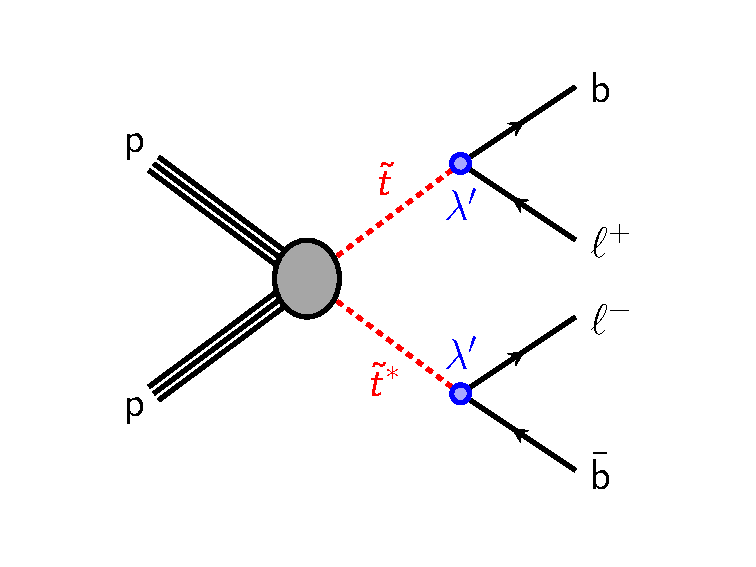
\includegraphics[width=0.60\textwidth]{figs/blstop/b_minus_l_stop_stop.pdf}
%   \caption{Simplified model of pair production of stop quarks, with decay to a
%     charged lepton and $b$-quark.
%   }
%   \label{fig:blstop_diagram}
% \end{figure}

%% -----------------------------------------------------------------------------
\FloatBarrier
\section{Signal model simulation}
\label{sec:signal_model_mc}

This search is optimized using Monte Carlo (MC) simulation of stop pair
production and decay.
Stop pair production is modeled using \madgraph\ version
1.5.12~\cite{Alwall:2011uj} to generate stop-anti-stop pairs using the
CTEQ 6L1 parton distribution functions (PDFs)~\cite{Nadolsky:2008zw},
and \pythia\ version 6.427~\cite{Sjostrand:2006za} to perform the
RPV stop decay as well as the parton shower calculation.
Stop pairs are generated for stop masses between 400~\GeV\ and 1100~\GeV\ in
steps of 100~\GeV.
Signal cross sections are calculated at next-to-leading order (NLO) in
$\alpha_s$, including the resummation of soft gluon emission at
next-to-leading-logarithm accuracy
(NLO+NLL)~\cite{Beenakker:1997ut,Beenakker:2010nq,Beenakker:2011fu}.
The nominal cross section and the uncertainty are taken from an envelope of
cross section predictions using different PDF sets and factorization and
renormalization scales, as described in Reference~\cite{Kramer:2012bx}.
The simulated stop cross section ranges from $356 \pm 51$~fb for a stop mass
of 400~\GeV\ to $0.18 \pm 0.06$~fb for a stop mass of 1100~\GeV.
The cross sections and associated uncertainties for stop pair production are
summarized in Table~\ref{tab:stop_xsec}.

All samples have been generated with stop branching fractions of 
$Br(\tilde{t} \rightarrow be) = Br(\tilde{t} \rightarrow b\mu) = 0.5$.
From this nominal branching fraction, the simulated events can be appropriately
weighted to give any branching fraction hypothesis.
This procedure is described in detail in
Section~\ref{sec:model_dependent_limits}
Except at high branching fraction for $Br(\tilde{t} \rightarrow b\tau)$,
$\tilde{t} \rightarrow b\tau$ decays do not significantly contribute to the
final state with two light leptons and two
$b$-jets.
This is due to the low branching fraction of
$\tau^{-} \rightarrow e^{-} \bar{\nu}_{e} \nu_{\tau}$ and 
$\tau^{-} \rightarrow \mu^{-} \bar{\nu}_{\mu} \nu_{\tau}$ (17\% each), as well
as the addition of neutrinos to the final state, leading to poorer mass
resolution on \MBL.
The decay $\tilde{t} \rightarrow b\tau$ does not significantly contribute to
the search sensitivity, and it is not included in the simulated samples.

\begin{table}[ht]
  \caption{Stop cross sections and their associated
    uncertainties~\cite{Beenakker:1997ut,Beenakker:2010nq,Beenakker:2011fu}.
  }
  \label{tab:stop_xsec}
  \centering{
    \begin{tabular}{ccc}
      % Stop Mass [\GeV] & Cross section [pb] & Uncertainty [pb] \\
      Stop Mass [\GeV] & Cross section [fb] & Uncertainty [pb] \\
      \midrule
      % 400  & $0.36$                & $0.05$               \\
      % 500  & $8.6  \times 10^{-2}$ & $1.3 \times 10^{-2}$ \\
      % 600  & $2.5  \times 10^{-2}$ & $4   \times 10^{-3}$ \\
      % 700  & $8.1  \times 10^{-3}$ & $1.5 \times 10^{-3}$ \\
      % 800  & $2.9  \times 10^{-3}$ & $6   \times 10^{-4}$ \\
      % 900  & $1.09 \times 10^{-3}$ & $2.6 \times 10^{-4}$ \\
      % 1000 & $4.4  \times 10^{-4}$ & $1.2 \times 10^{-4}$ \\
      % 1100 & $1.8  \times 10^{-4}$ & $6   \times 10^{-5}$ \\
      400  & $360$  & $50$   \\
      500  & $86$   & $130$  \\
      600  & $25$   & $4$    \\
      700  & $8.1$  & $1.5$  \\
      800  & $2.9$  & $0.6$  \\
      900  & $1.1$  & $0.3$  \\
      1000 & $0.44$ & $0.12$ \\
      1100 & $0.18$ & $0.06$ \\
      \bottomrule
    \end{tabular}
  }
\end{table}

%% -----------------------------------------------------------------------------
\FloatBarrier
\section{Object selection}
\label{sec:object_selection}

Events are required to have at least two light leptons (electrons or muons)
with opposite charge, and two $b$-tagged jets.
The object selection is performed in multiple steps. First, lepton and jet
objects are reconstructed using detector signatures as described in
\cref{sec:elctrons,sec:muons,sec:jets}.
Baseline requirements are applied to remove poorly reconstructed objects.
All baseline objects are required to have $\ET(\pt) \geq 40 \GeV$ since the
stop signatures of interest are of high mass and produce high momentum decay
products.

%% - - - - - - - - - - - - - - - - - - - - - - - - - - - - - - - - - - - - - - -
%% baseline electrons
%% - - - - - - - - - - - - - - - - - - - - - - - - - - - - - - - - - - - - - - -
Baseline electrons must satisfy the \texttt{Medium++} identification
requirement and have $|\eta| \leq 2.47$.
A requirement of $\DZEROSIG \leq 3$ and
$\ZZEROSINTHETA \leq 0.4$ mm is placed on the impact parameter
to reject electrons coming from the decay of long-lived particles.
The baseline electron requirements are outlined in
Table~\ref{tab:baseline_el_def}.

\begin{table}[ht]
\caption{Baseline electron requirements.}
\label{tab:baseline_el_def}
\centering{
  \begin{tabular}{cc}
    \toprule
    Quality        & \texttt{Medium++} \\
    $p_T$          & $\geq 40 \GeV$    \\
    $|\eta|$       & $\leq 2.47$       \\
    \DZEROSIG      & $\leq 3$          \\
    \ZZEROSINTHETA & $\leq 0.4$ mm     \\
    \bottomrule
  \end{tabular}
}
\end{table}

%% - - - - - - - - - - - - - - - - - - - - - - - - - - - - - - - - - - - - - - -
%% baseline muons
%% - - - - - - - - - - - - - - - - - - - - - - - - - - - - - - - - - - - - - - -
Baseline muons are selected from the \texttt{STACO} muon collection, and
required to pass the \texttt{Loose} identification requirement. The baseline
muons must also have $|\eta| \leq 2.5$.
Impact parameter requirements of $\DZEROSIG \leq 3$ and
$\ZZEROSINTHETA \leq 1$ mm are applied to reduce the contamination of muons
from secondary vertices and cosmic rays.
Additional requirements are applied on the number of hits in the ID to ensure
high quality tracks.
These  hit requirements include at least one hit on track in both the B layer
and the Pixel detector.
The ID track must also have at least 5 hits in the SCT, and at most 2 missing 
hits-on-track (holes) in both the Pixel detector and the SCT. 
If the muon has $|\eta| \leq 1.9$, there must additionally be at least 6 TRT
hits, of which no more than 90\% are outliers.
The baseline muon requirements are outlined in Table~\ref{tab:baseline_mu_def}.

\begin{table}[ht]
  \caption{Baseline muon requirements.}
  \label{tab:baseline_mu_def}
  \centering{
    \begin{tabular}{cc}
      \toprule
      Quality              & \texttt{Loose} \\
      $p_T$                & $\geq 40 \GeV$ \\
      $|\eta|$             & $\leq 2.5$     \\
      Number B layer hits  & $\geq 1$       \\
      Number Pixel hits    & $\geq 1$       \\
      Number SCT hits      & $\geq 5$       \\
      Number Silicon holes & $\leq 2$       \\
      TRT hits             & See text       \\
      \DZEROSIG            & $\leq 3$       \\
      \ZZEROSINTHETA       & $\leq 1$ mm    \\
      \bottomrule
    \end{tabular}
  }
\end{table}

%% - - - - - - - - - - - - - - - - - - - - - - - - - - - - - - - - - - - - - - -
%% baseline jets
%% - - - - - - - - - - - - - - - - - - - - - - - - - - - - - - - - - - - - - - -
Baseline jets are selected from the AntiKt4LCTopo jet collection, which apply a
and required to have $|\eta| \leq 4.9$.
These jets are build using the anti-$k_\mathrm{T}$ jet clustering algorithm
with a cone size of $\Delta R \leq 0.4$~\cite{Cacciari:2008gp}.
The baseline jet requirements are outlined in Table~\ref{tab:baseline_jet_def}.

\begin{table}[ht]
    \caption{Baseline jet requirements.}
    \label{tab:baseline_jet_def}
  \centering{
    \begin{tabular}{cc}
      \toprule
      $p_T$    & $\geq 40 \GeV$ \\
      $|\eta|$ & $\leq 4.9$     \\
      \bottomrule
    \end{tabular}
  }
\end{table}

%% - - - - - - - - - - - - - - - - - - - - - - - - - - - - - - - - - - - - - - -
%% overlap removal
%% - - - - - - - - - - - - - - - - - - - - - - - - - - - - - - - - - - - - - - -
The overlap between baseline objects is removed to prevent a single
detector signature from being included in multiple particle
collections.~\footnote{The angular separation between the objects is measured
as $\Delta R = \sqrt{(\Delta \phi)^2 + (\Delta \eta)^2}$}

\begin{enumerate}
  \item $\Delta R(e,e) \le 0.05$: If two baseline electrons fall
    within a cone of $\Delta R(e,e) \le 0.05$, the electron with the
    lower \ET\ is removed from the event.
  \item $\Delta R(e,\mathrm{jet}) \le 0.20$: If a remaining electron and a jet
    are within a cone of $\Delta R(e,\mathrm{jet}) \le 0.20$, it is
    assumed that the electron is also reconstructed as a jet, and the
    jet is removed from the event.
  \item $\Delta R(\ell,\mathrm{jet}) \le 0.40$: If remaining lepton (electron
    or muon) is within a cone of $\Delta R(\ell,\mathrm{jet}) \le 0.40$ of a
    remaining jet, the reconstructed lepton is assumed to be a constituent of
    the jet, and is removed from the event.
  \item $\Delta R(e,\mu) \le 0.01$: If a remaining electron and a remaining muon
    are within $\Delta R(e,\mu) \le 0.01$, both are removed from the event.
  \item $\Delta R(\mu,\mu) \le 0.05$: If two remaining muons are within
    $\Delta R(\mu,\mu) \le 0.05$, both are removed from the event.
\end{enumerate}

Leptons from the decays of low hadronic mass resonances are rejected.
The invariant mass of any remaining same-flavor lepton pairs with opposite
charge is computed, and if the invariant mass of any of these pairs is less
than 12~\GeV, both leptons are removed from the event.

%% - - - - - - - - - - - - - - - - - - - - - - - - - - - - - - - - - - - - - - -
%% signal object definitions
%% - - - - - - - - - - - - - - - - - - - - - - - - - - - - - - - - - - - - - - -
Additional requirements are placed on the leptons and jets after overlap
removal to select the final ``signal'' objects.
The scalar sum of the transverse momentum of all tracks with $\pt \geq 400 \MeV$
within a cone of $\Delta R \leq 0.30$ of a lepton ($\pt^\mathrm{cone30}$) is
used to determine if the lepton is isolated.
Both electrons and muons require
$\nicefrac{\pT^{\mathrm{cone30}}}{\min(p_T, 60\,\GeV)} \leq 0.1$ in order
to be declared signal leptons.
Signal jets must be within $|\eta| \leq 2.4$, and be tagged as a $b$-jet
according to the MV1 flavor tagging
algorithm~\cite{ATLAS-CONF-2014-004, ATLAS-CONF-2014-046}.
The operating point of $\mathrm{MV1} \geq 0.3511$ corresponds to an overall
80\% $b$-tagging efficiency, as measured in simulated \TTBAR\ events, to a
rejection factor of 25 for jets originating from light quarks or gluons, and to
a rejection factor of 3 for jets originating from charm quarks.

Events must contain at least two signal leptons and two $b$-tagged jets.
If more are found, the event is kept, but only the two signal leptons and two
$b$-tagged jets with the highest \ET(\pt) are selected.
Furthermore, the two highest \ET(\pt) leptons are required to have opposite charge.

The identification efficiencies for the various objects used in this analysis
differ in the data and the MC simulation.
The efficiencies are determined in both data and MC simulation, by the relevant
ATLAS performance working groups~\cite{egamma2014,Aad:2014rra}.
The lepton identification scale factors and are computed for each of the two
signal leptons in a MC simulated event, and depend on both the
\pt\ and \eta\ of the leptons.
The product of the scale factors is taken as an event weight, ranging from
{\color{red} TODO find the range of lepton SF event weights}.

Data and MC simulation also have different efficiencies for tagging a $b$-jet
and for misidentifying jets originating from the fragmentation of light-flavor
quarks, gluons, and charm quarks. 
An individual jet scale factor is defined as
\begin{equation}
  SF_\mathrm{jet}^\mathrm{eff}
  =
  \frac{\epsilon_\mathrm{jet}^\mathrm{data}}{\epsilon_\mathrm{jet}^\mathrm{MC}},
\end{equation}
and depends on the \et, \eta, and truth flavor of the jet.
The individual jet scale factor is calculated for each of the baseline jets in
a MC simulated event, and the overall event level $b$-tagging scale factor is
given by 
\begin{equation}
  \label{eqn:b_tag_sf}
  SF_{b\mathrm{-tagging}}^\mathrm{event} =
  \prod_{i \in \mathrm{tagged}}
  SF_i^\mathrm{eff}
  \times
  \prod_{j \in \mathrm{Not~tagged}}
  (1- SF_j^\mathrm{eff}),
\end{equation}
where $SF_i^\mathrm{eff}$ is the tagging efficiency scale factor of jet $i$, and
$(1- SF_j^\mathrm{eff})$ is the rejection efficiency for jet $j$.
The two terms in equation~\ref{eqn:b_tag_sf}, are the products over the
$b$-tagged and non-$b$-tagged jets in the event respectively.
This $SF_{b\mathrm{-tagging}}^\mathrm{event}$ quantity is taken as an additional
event weight in MC simulated events.

%% - - - - - - - - - - - - - - - - - - - - - - - - - - - - - - - - - - - - - - -
%% pairing
%% - - - - - - - - - - - - - - - - - - - - - - - - - - - - - - - - - - - - - - -
A pairing of leptons and $b$-tagged jets must be defined to construct the mass
of each of the $b\ell$ pairs in a event.
In the target signal model, each $b\ell$ pair comes from a resonant decay of a
stop particle with the same invariant mass.
Therefore, the pairing which minimizes the difference in mass between the two
$b\ell$ pairs is selected as follows.

In order of decreasing \pt, the two signal leptons and two $b$-jets are
labeled $\ell_0$, $\ell_1$, $b_0$, and $b_1$.

% Define some colors for this section to make changing colors easier
\colorlet{pairing_l_0}{green!50!white}
\colorlet{pairing_l_1}{green!20!white}
\colorlet{pairing_b_0}{red!50!white}
\colorlet{pairing_b_1}{red!20!white}
%
% \begin{center}
%   \begin{tikzpicture}
%     \node[rectangle, rounded corners=1ex, fill=pairing_b_0, text=black]
%       (b0) at (-3,0) {$b_0$};
%     \node[rectangle, rounded corners=1ex, fill=pairing_b_1, text=black]
%       (b1) at (-1,0) {$b_1$};
%     \node[rectangle, rounded corners=1ex, fill=pairing_l_0, text=black]
%       (l0) at (+1,0) {$\ell_0$};
%     \node[rectangle, rounded corners=1ex, fill=pairing_l_1, text=black]
%       (l1) at (+3,0) {$\ell_1$};
%   \end{tikzpicture}
% \end{center}
%
There are two possible choices of pairings for these four objects:
%
\begin{center}
  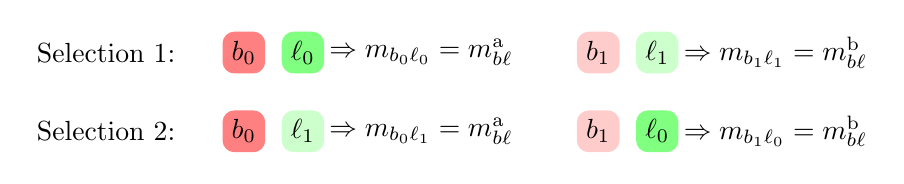
\begin{tikzpicture}
    \node[rectangle, text=black] (sel1) at (-5.0,+0.5) {Selection 1:};
    \node[rectangle, text=black] (sel2) at (-5.0,-0.5) {Selection 2:};

    \node[rectangle, rounded corners=1ex, fill=pairing_b_0, text=black]
      (b1) at (-3.25,+0.5) {$b_0$};
    \node[rectangle, rounded corners=1ex, fill=pairing_l_0, text=black]
      (l0) at (-2.50,+0.5) {$\ell_0$};
    \node[rectangle, rounded corners=1ex, fill=pairing_b_1, text=black]
      (b1) at (+1.25,+0.5) {$b_1$};
    \node[rectangle, rounded corners=1ex, fill=pairing_l_1, text=black]
      (l1) at (+2.00,+0.5) {$\ell_1$};
    \node[rectangle, text=black]
      (m00) at (-1.0,+0.5)
      {$\Rightarrow m_{b_0\ell_0} = m_{b\ell}^\mathrm{a}$};
    \node[rectangle, text=black]
      (m11) at (+3.5,+0.5)
      {$\Rightarrow m_{b_1\ell_1} = m_{b\ell}^\mathrm{b}$};

    \node[rectangle, rounded corners=1ex, fill=pairing_b_0, text=black]
      (b0) at (-3.25,-0.5) {$b_0$};
    \node[rectangle, rounded corners=1ex, fill=pairing_l_1, text=black]
      (l1) at (-2.50,-0.5) {$\ell_1$};
    \node[rectangle, rounded corners=1ex, fill=pairing_b_1, text=black]
      (b1) at (+1.25,-0.5) {$b_1$};
    \node[rectangle, rounded corners=1ex, fill=pairing_l_0, text=black]
      (l0) at (+2.00,-0.5) {$\ell_0$};
    \node[rectangle, text=black]
      (m01) at (-1.0,-0.5)
      {$\Rightarrow m_{b_0\ell_1} = m_{b\ell}^\mathrm{a} $};
    \node[rectangle, text=black]
      (m10) at (+3.5,-0.5)
      {$\Rightarrow m_{b_1\ell_0} = m_{b\ell}^\mathrm{b} $};
  \end{tikzpicture}
\end{center}

The choice that gives the
smallest difference in the mass $|\MBL^\mathrm{a} - \MBL^\mathrm{b}|$
is chosen.
The pairs are then ordered, and relabeled such that the higher mass pair has a
mass of $\MBL^{0}$, and the lower mass pair has a mass of $\MBL^{1}$.
This ensures $\MBL^{0} \geq \MBL^{1}$ by definition.

This heuristic correctly identifies at least one correct pairing in over
70\% of events in the simulated signal samples
depending on the mass of the simulated stop. The relative abundance of
identifying both, only one, or no correct pairs in simulated stop events is
shown in Figure~\ref{fig:pairing_eff}.
The efficiency of identifying correct pairs improves once a cut is applied on
the mass asymmetry of the two $b\ell$ pairs as described in
Section~\ref{sec:signal_regions}.
The scenario where one of the $b$-tagged jets or one of the leptons is not
matched to a stop parent.

\begin{figure}[ht]
  \centering
  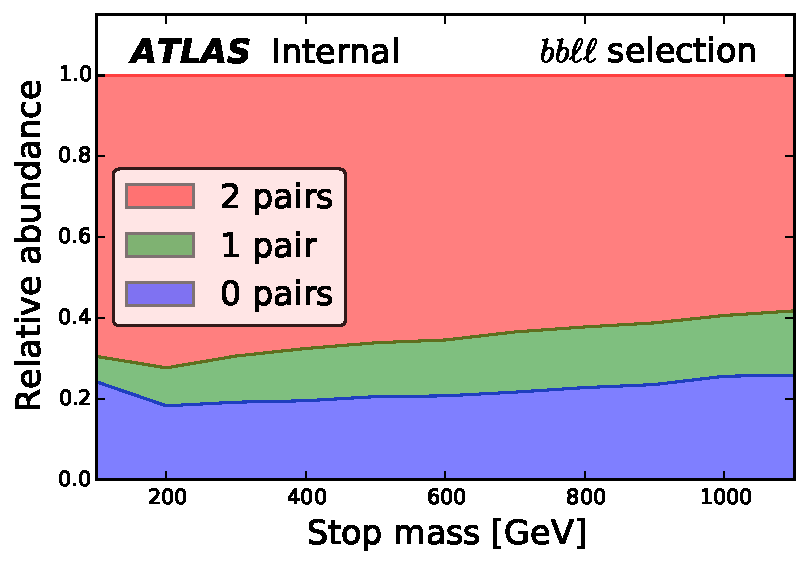
\includegraphics[width=0.75\textwidth]
    {figs/blstop/PairingEfficiencies/pairing_abundance__inclusive.pdf}
  \caption{The relative abundance of events where two, one, and zero
    pairs are grouped correctly.
  }
  \label{fig:pairing_eff}
\end{figure}

%% -----------------------------------------------------------------------------
\FloatBarrier
\section{Event cleaning}
\label{sec:event_cleaning}

All sub-systems of the ATLAS detector are required to be operating acceptably
during data-taking. 
This data quality requirement is implemented using a good runs list (GRL)
provided by the Data Preparation group.\footnote{The GRL version
\texttt{data12\_8TeV.periodAllYear\_DetStatus-v61-pro14-02\_DQDefects-00-01-00\_PHYS\_StandardGRL\_All\_Good}
is used.}
By applying the GRL requirement, the total integrated luminosity is reduced
from 21.4~\ifb\ to 20.3~\ifb.
The uncertainty in the luminosity is $\pm 2.8$\%.
It is derived following the same methodology as that detailed
in Reference~\cite{Lumi}.
The GRL requirement is applied to data events only; the MC simulation samples
are scaled to match the target luminosity.
Each event is also required to have at least one primary vertex with at least
5 associated tracks.

% Several other detector errors can lead to an event being rejected.
In the event of a certain detector busy condition, the Timing, Trigger, and
Control system (TTC) may be restarted in order to recover the detector without
a full run-restart.
In the lumi-block after a TTC restart, it is possible for stored events to be
incomplete.
For this reason, events stored immediately after a TTC restart are rejected.
Events are also rejected if either the LAr or tile calorimeter is
flagged as having an error.
During periods G-J several events are corrupt in a single channel of the tile
calorimeter, but not flagged as having a tile calorimeter error.
These events are also rejected using the \texttt{TileTripTool}.
During period B a hot spot developed in the tile calorimeter.
As this can negatively impact the jet calibration and the \met calculations,
events with a jet pointing toward this hot spot in the tile calorimeter are
rejected.

Jet cleaning is performed to flag jets which are formed from various sources
such as hardware problems, LHC beam conditions, or cosmic ray showers rather
than real energy deposits in the calorimeter.
If any of these bad jets remain after the overlap removal procedure, the event
is rejected.
Additionally, during periods E-H, a region of the LAr
calorimeter ($-0.1\le\eta\le1.5$ and $-0.9\le\phi\le-0.5$) malfunctioned
resulting in energy not being collected from electrons and jets, and
indirectly changing the \met\ measurement.
A correction is applied to jets to account for the energy loss,
however, if the correction is too large (greater than 0.05) and the \met\ is
close to the jet ($\Delta\phi(\met, \text{jet}) \le 0.3$), it is assumed the
\met\ is mismeasured, and the event is rejected.

In addition to the impact parameter significance requirement on signal muons
discussed in Section~\ref{sec:object_selection}, an additional requirement of
$|d_0| \leq 0.2$~mm is applied to muons passing the overlap removal to reject
muons from cosmic ray showers. Any event failing this selection requirement is
rejected.
In order to ensure muons are well measured, any event containing a muon after
overlap removal with $\nicefrac{\sigma_{q/p}}{|q/p|} > 0.2$ is rejected.
These poorly measured muons can arise from the MS and ID reconstructing
different momenta for the same muon.

An additional requirement is applied to MC simulation events to avoid double
counting backgrounds with heavy flavor quarks in the final state, the heavy
flavor overlap removal procedure, described in Section~\ref{sec:jet_matching}.

Events in data are taken from both the \texttt{egamma} and \texttt{muons} data
streams.
It is possible for the same event to exist in both streams, in particular for
$e\mu$ events, leading to the potential double counting of events in data.
To prevent this double counting of data events, the data stream is chosen based
on the flavor of the leading signal lepton in the event.
If the highest \pt\ lepton in the event is an electron (muon), the event is
required to be found in the \texttt{egamma} (\texttt{muons}) data stream.
Events found in the wrong stream, are rejected.

%% -----------------------------------------------------------------------------
\FloatBarrier
\section{Trigger selection}
\label{sec:trigger_selection}

A combination of four single-lepton triggers are used to select events.
The specific triggers used depend on the flavor channel of the event.
Di-electron(muon) events are required to pass at least one of the two single
electron (muon) triggers, while electron-muon events may pass any one of the
four triggers.
The specific triggers used for each flavor channel are outlined in
Table~\ref{tab:triggers}, and the trigger requirements are described in
Table~\ref{tab:trigger_defs}.

\begin{table}[ht]
  % \caption{Trigger selection for each final state. If the event passes any of
  %   the triggers for the given final state, the event is accepted.
  % }
  \caption[Trigger selection for each final state.]{Trigger selection for each final state. If the event passes any of
    the triggers for the given final state, the event is accepted.
  }
  \label{tab:triggers}
  \centering{
    \begin{tabular}{cc}
      \toprule
      Final state & Trigger \\
      \midrule
      \multirow{2}{*}{$ee$bb}     &  \texttt{EF\_e24vhi\_medium1} \\
                                  &  \texttt{EF\_e60\_medium1}    \\
      \midrule
      $\mu\mu$bb                  &  \texttt{EF\_mu24i\_tight}    \\
      $\mu\mu$bb                  &  \texttt{EF\_mu36\_tight}     \\
      \midrule
      \multirow{3}{*}{$e\mu$bb}   &  \texttt{EF\_e24vhi\_medium1} \\
                                  &  \texttt{EF\_e60\_medium1}    \\
                                  &  \texttt{EF\_mu24i\_tight}    \\
                                  &  \texttt{EF\_mu36\_tight}     \\
      \bottomrule
    \end{tabular}
  }
\end{table}

\begin{table}[ht]
    \caption{Requirements for the triggers used in this analysis.  }
    \label{tab:trigger_defs}
  \centering{
    \begin{tabular}{c|cc}
      \toprule
      Trigger & \pt\ threshold & Other requirements \\
      \midrule
      \multirow{2}{*}{\texttt{EF\_e24vhi\_medium1}}
      & \multirow{2}{*}{$\pt^{e} \geq 24 \GeV$}
      & hadronic core isolation $\leq 1 \GeV$ \\
      & & $\nicefrac{\pt^\mathrm{cone20}}{\pt} < 0.1$ \\ [1ex]
      \texttt{EF\_e60\_medium1} & $\pt^{e} \geq 60 \GeV$ & -- \\ [1ex]
      \texttt{EF\_mu24i\_tight}
      & $\pt^{e} \geq 24 \GeV$
      & $\nicefrac{\pt^\mathrm{cone20}}{\pt} < 0.12$ \\ [1ex]
      \texttt{EF\_mu36\_tight}  & $\pt^{e} \geq 36 \GeV$ & -- \\ [1ex]
      \bottomrule
    \end{tabular}
  }
\end{table}

At least one of the reconstructed leptons is required to be within 
$\Delta R \leq 0.15$ of the detector signature found by the trigger.
A reconstructed lepton must be matched to a trigger object of the correct flavor.
For example, a reconstructed electron which is very close to a muon trigger
object is not considered matched for these purposes.
The expected trigger efficiencies for simulated stop events are shown
for each trigger individually in Figure~\ref{fig:single_trigger_efficiency}.
The two muon triggers have roughly the same trigger efficiency, of about 93\% 
for $\mu\mu$ events and 75\% for $e\mu$ events, for all stop masses.
The two electron triggers, however, have dramatically different shapes.
The \texttt{EF\_e24vhi\_medium1} trigger is highly efficient for $ee$ and
$e\mu$ events only at low stop mass values.
The \texttt{EF\_e60\_medium1} trigger only reaches 95\% efficiency for
$ee$ and $e\mu$ events from stops with $m_{\tilde{t}} > 200 \GeV$.
Due to the trigger requirement, and the overlap removal procedure,
$ee$~($\mu\mu$) events do not pass the single muon (electron) triggers.

The dependence on the stop mass is a result of the \ET\ dependence of the
electron triggers.
The decay products of lighter stops tend to have lower momentum.
As a result, the electrons from the very light stops ($\leq 300~\GeV$) 
are more likely to have \ET\ less than the threshold for the
\texttt{EF\_e60\_medium1} trigger.
High-\ET\ electrons will deposit more energy into the calorimeter,
and some of this energy will reach the hadronic calorimeter.
As the electron \ET\ increases, the probability that the energy deposition into
the hadronic calorimeter is enough to fail the hadronic core isolation
requirement of the \texttt{EF\_e24vhi\_medium1} trigger increases.
The \ET\ dependence of the two electron triggers, shown in
Figure~\ref{fig:electron_trigger_pt_dependence}, is consistent with the expected
dependence.

\begin{figure}[ht]
  \centering
  \subbottom[\texttt{EF\_e24vhi\_medium1}]{
    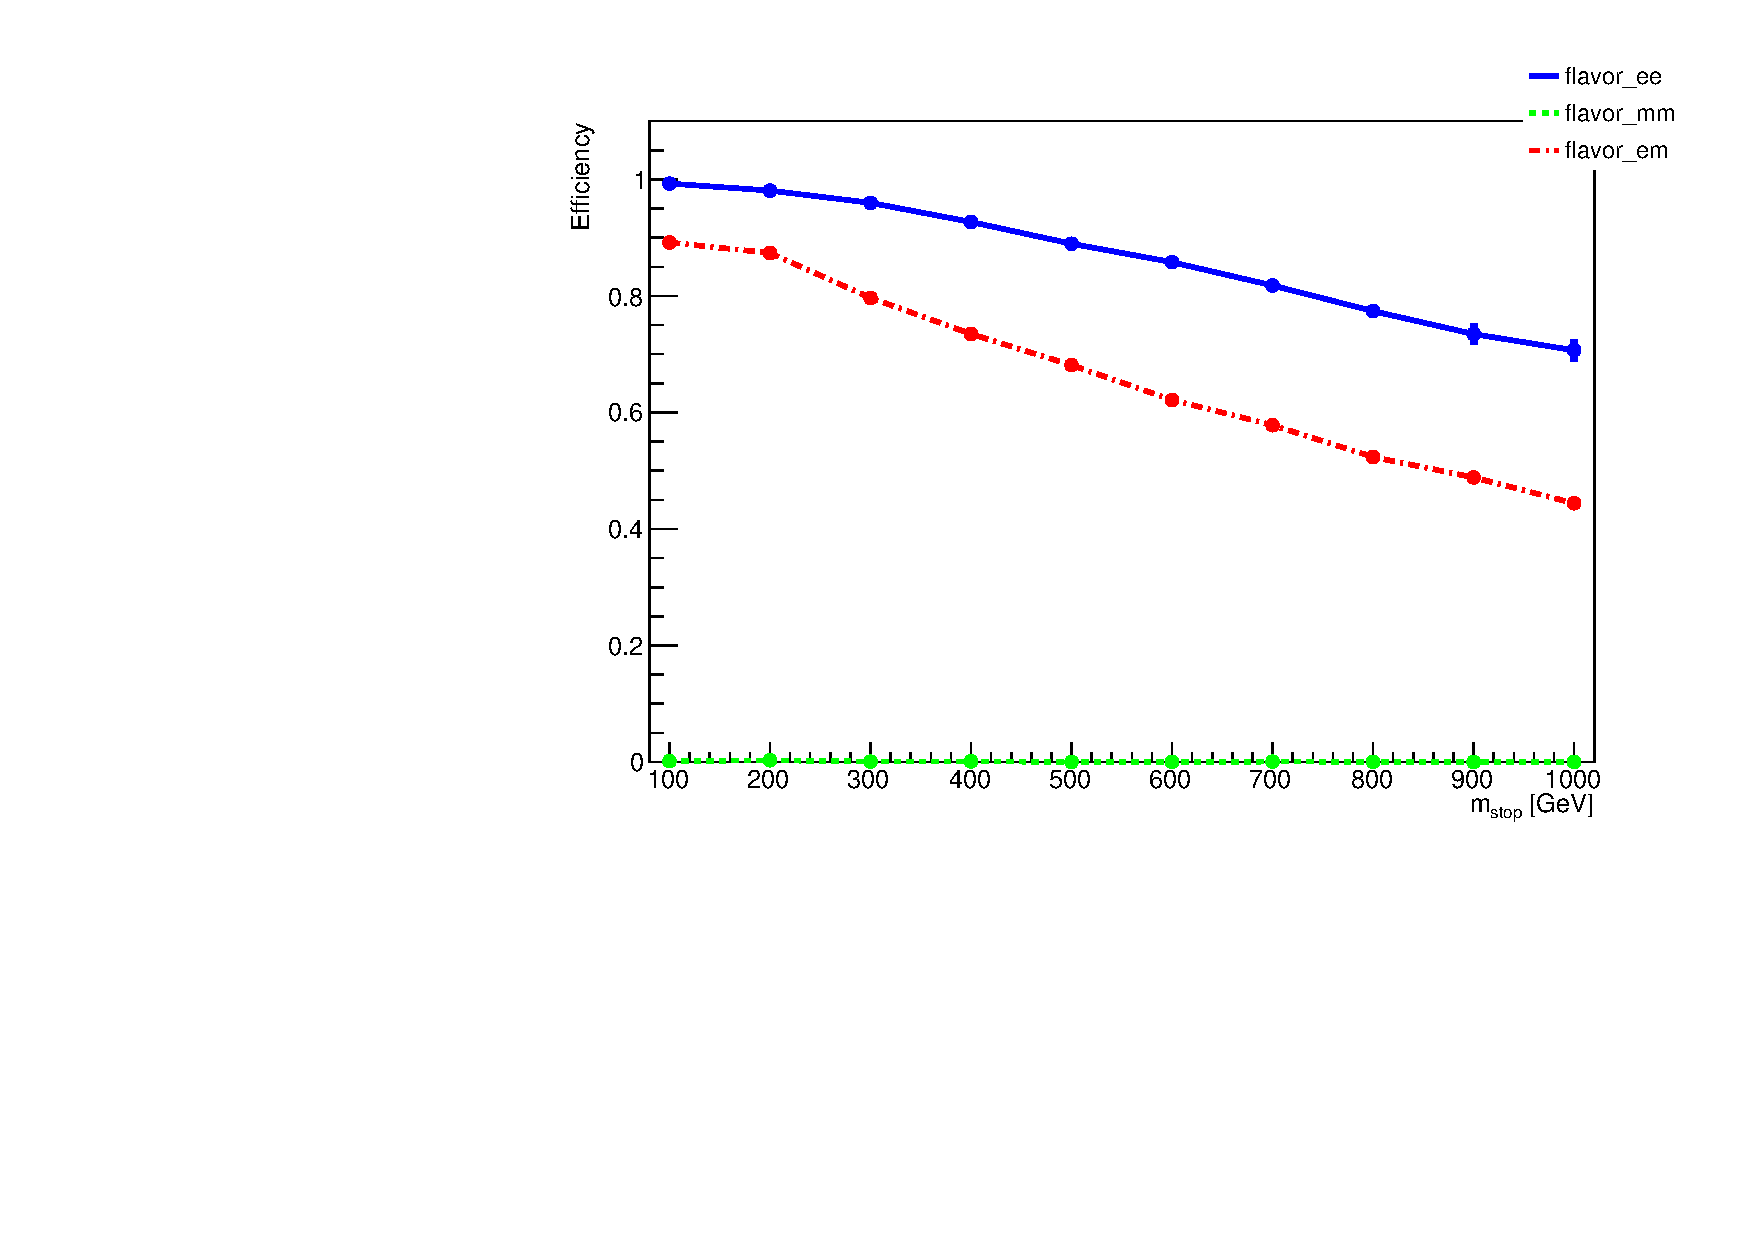
\includegraphics[width=0.48\textwidth]
      {figs/trigger/EF_e24vhi_medium1.pdf}
  }
  \subbottom[\texttt{EF\_e60\_medium1}]{
    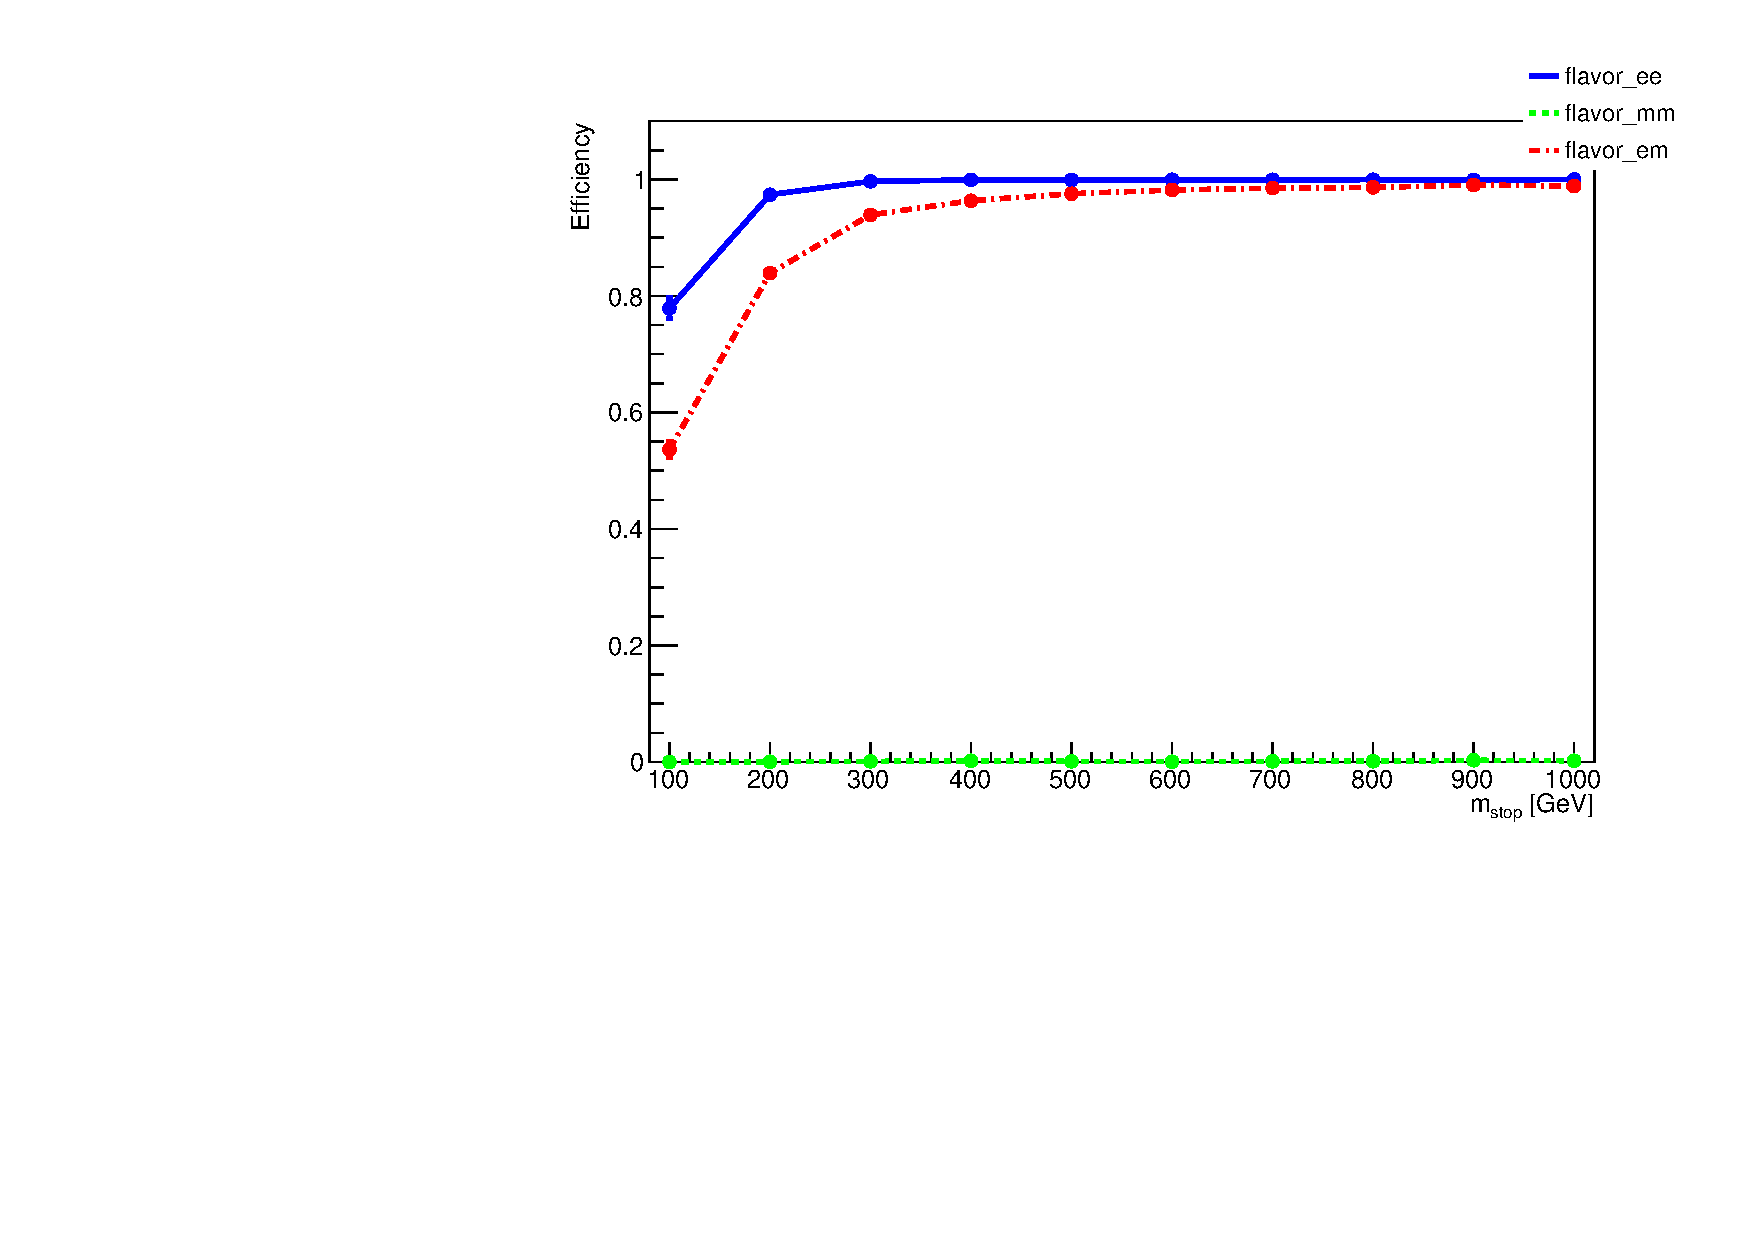
\includegraphics[width=0.48\textwidth]
      {figs/trigger/EF_e60_medium1.pdf}
  }
  \subbottom[\texttt{EF\_mu24i\_tight trigger}]{
    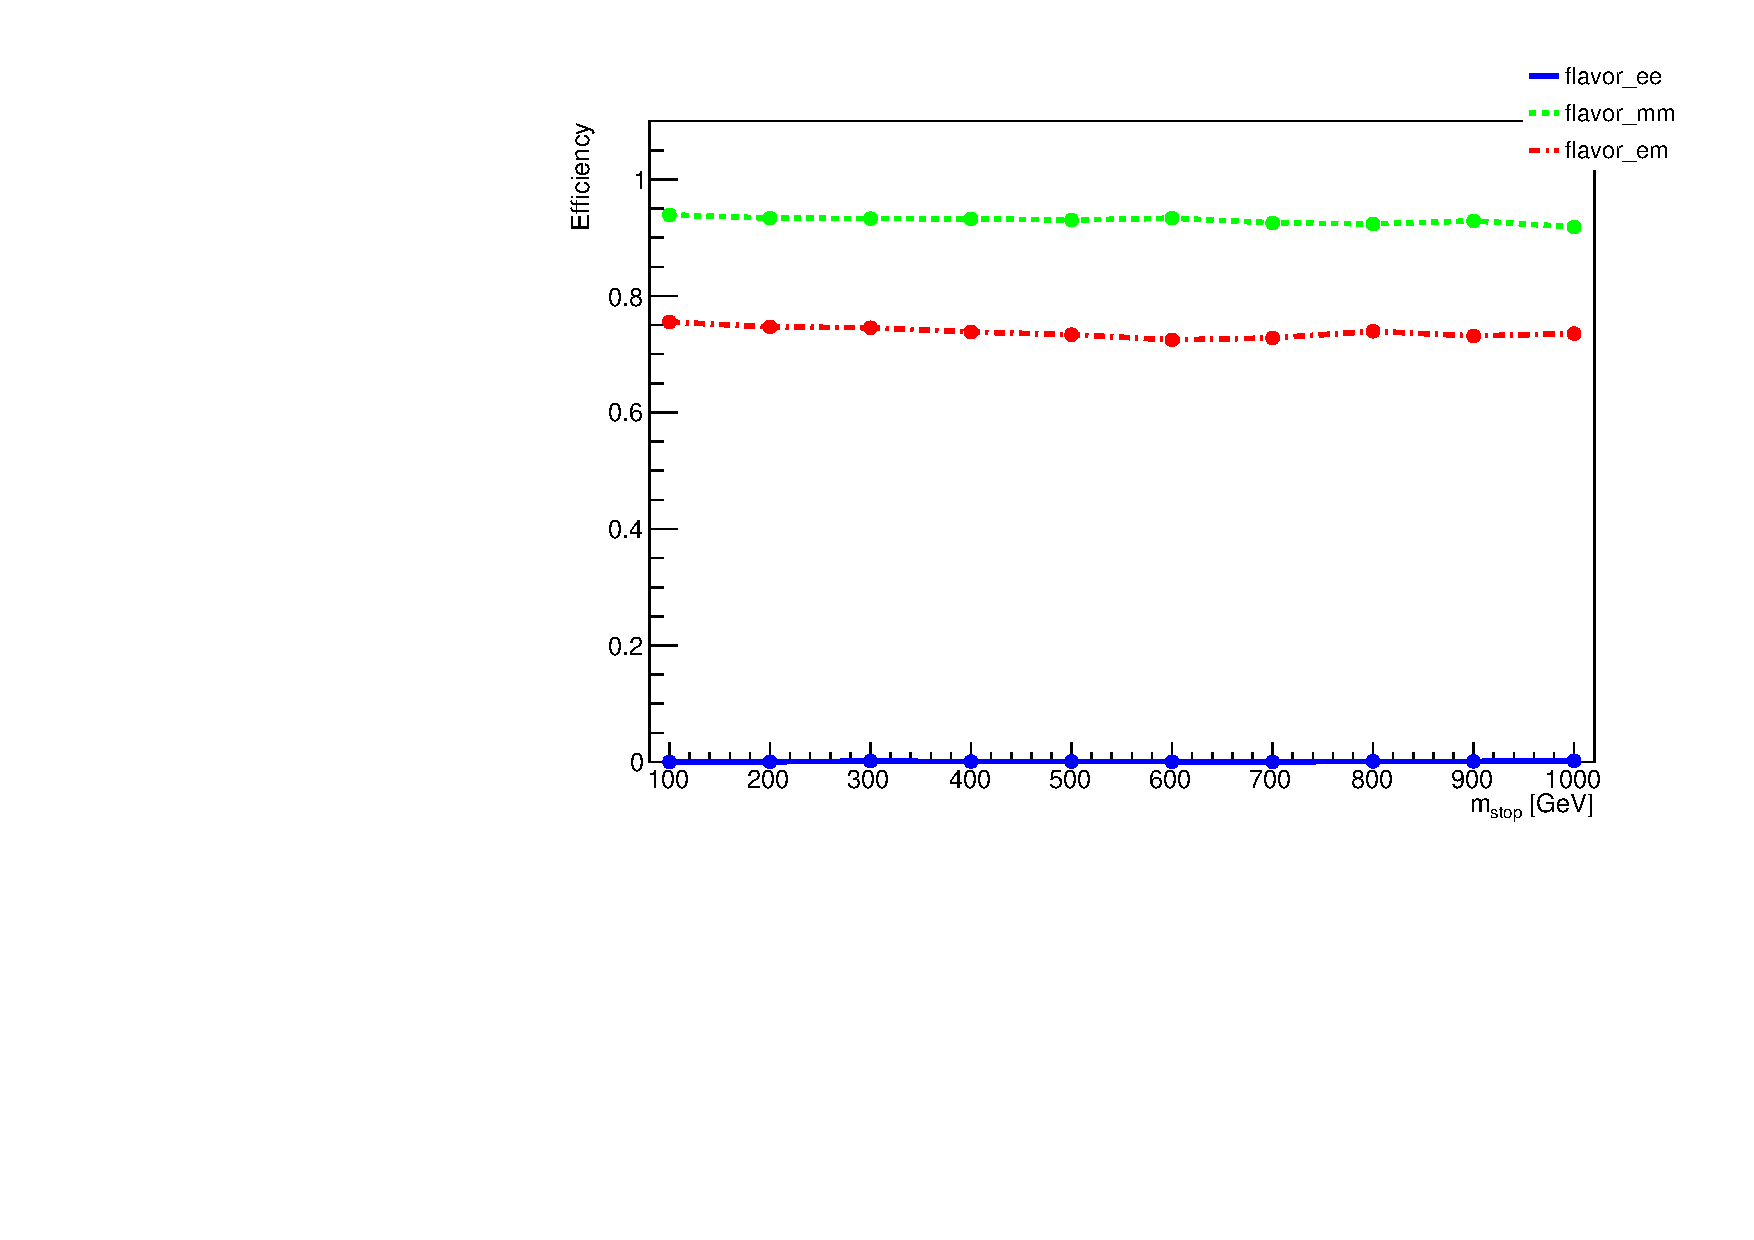
\includegraphics[width=0.48\textwidth]
      {figs/trigger/EF_mu24i_tight.pdf}
  }
  \subbottom[\texttt{EF\_mu36\_tight}]{
    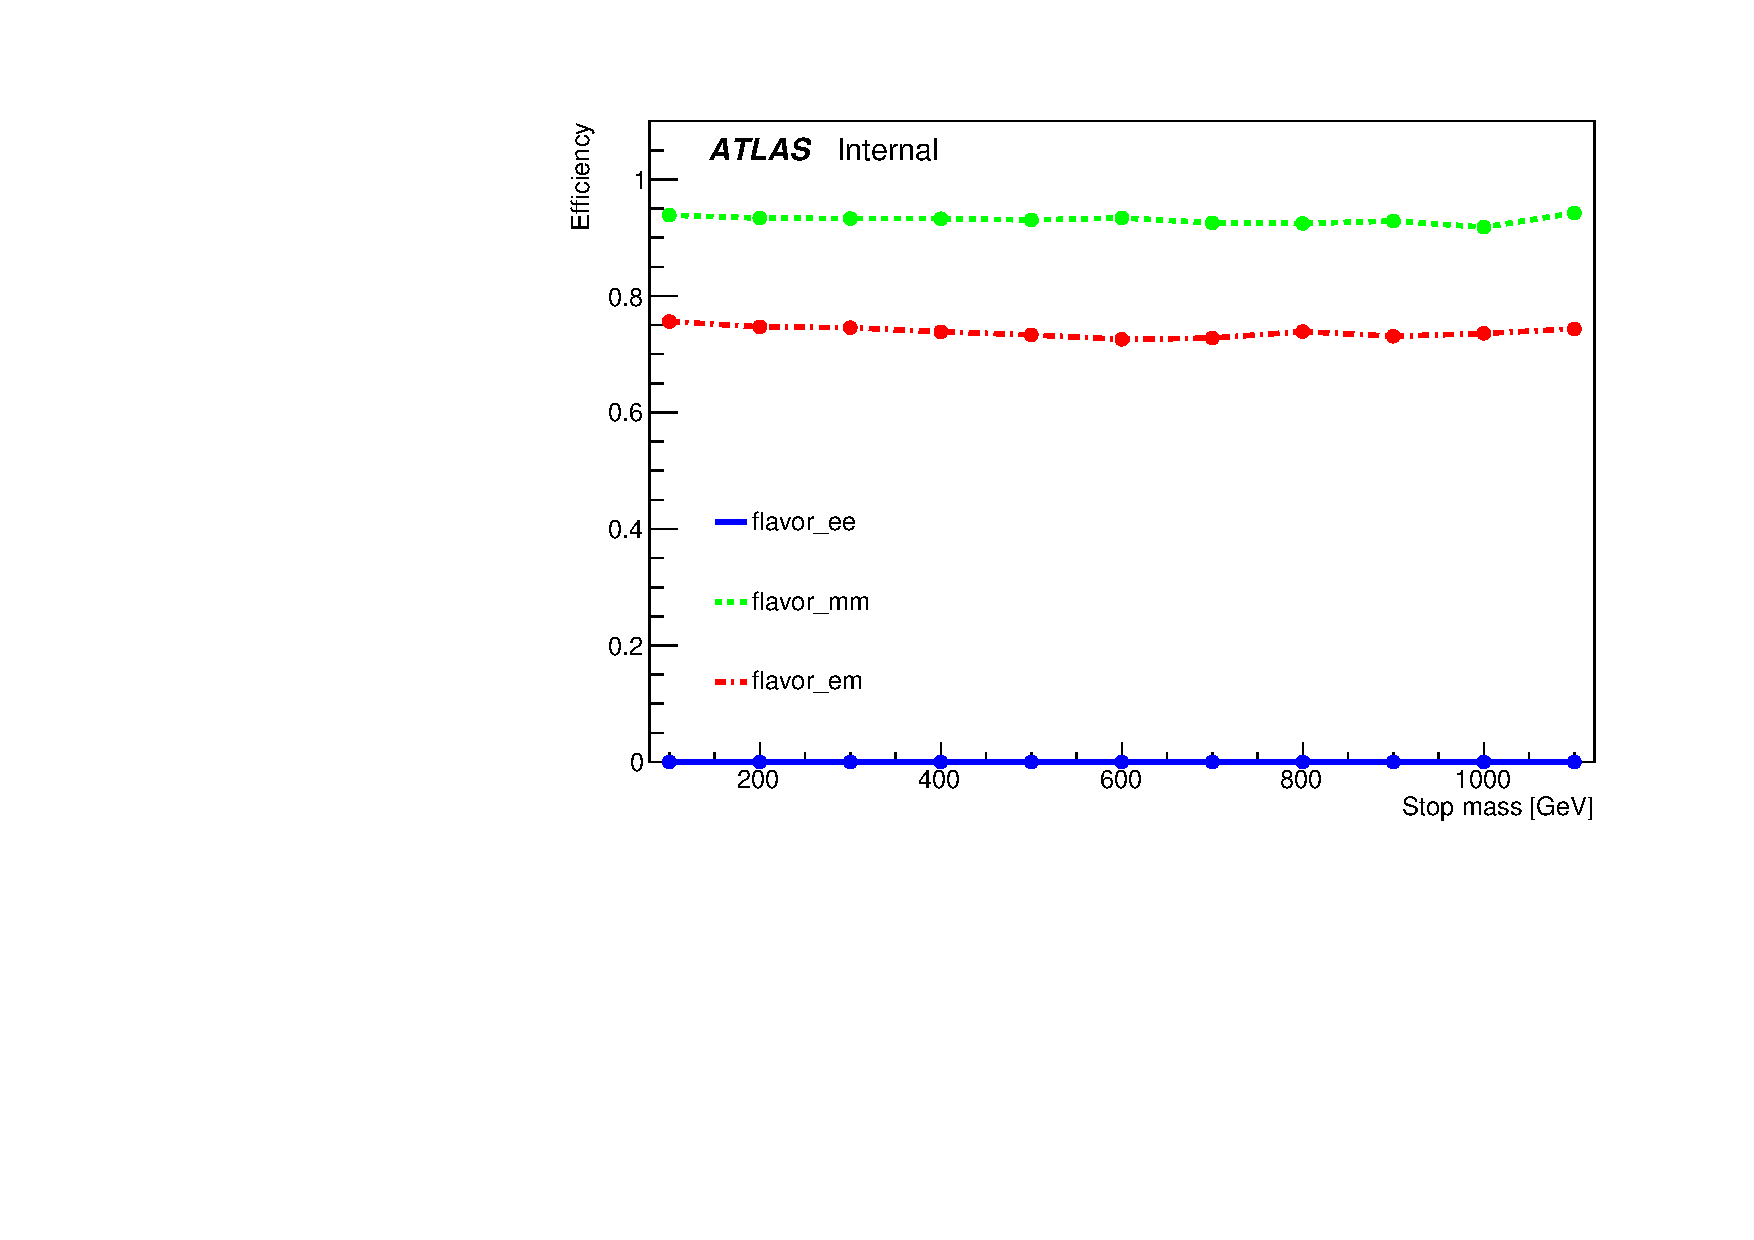
\includegraphics[width=0.48\textwidth]
      {figs/trigger/EF_mu36_tight.pdf}
  }
  \caption{Efficiency of simulated stop events passing each single lepton
    trigger broken down by flavor channel.
    % The two single electron triggers have different shapes, which the 
    % \texttt{EF\_e24vhi\_medium1} trigger being more efficient for low stop
    % masses and the \texttt{EF\_e60\_medium1} trigger more efficient for
    % higher stop masses.
    % The two single muon triggers have roughly equal efficiency for all stop
    % masses.
  }
  \label{fig:single_trigger_efficiency}
\end{figure}

\begin{figure}[ht]
  \centering
  \subbottom[\texttt{EF\_e24vhi\_medium1}]{
    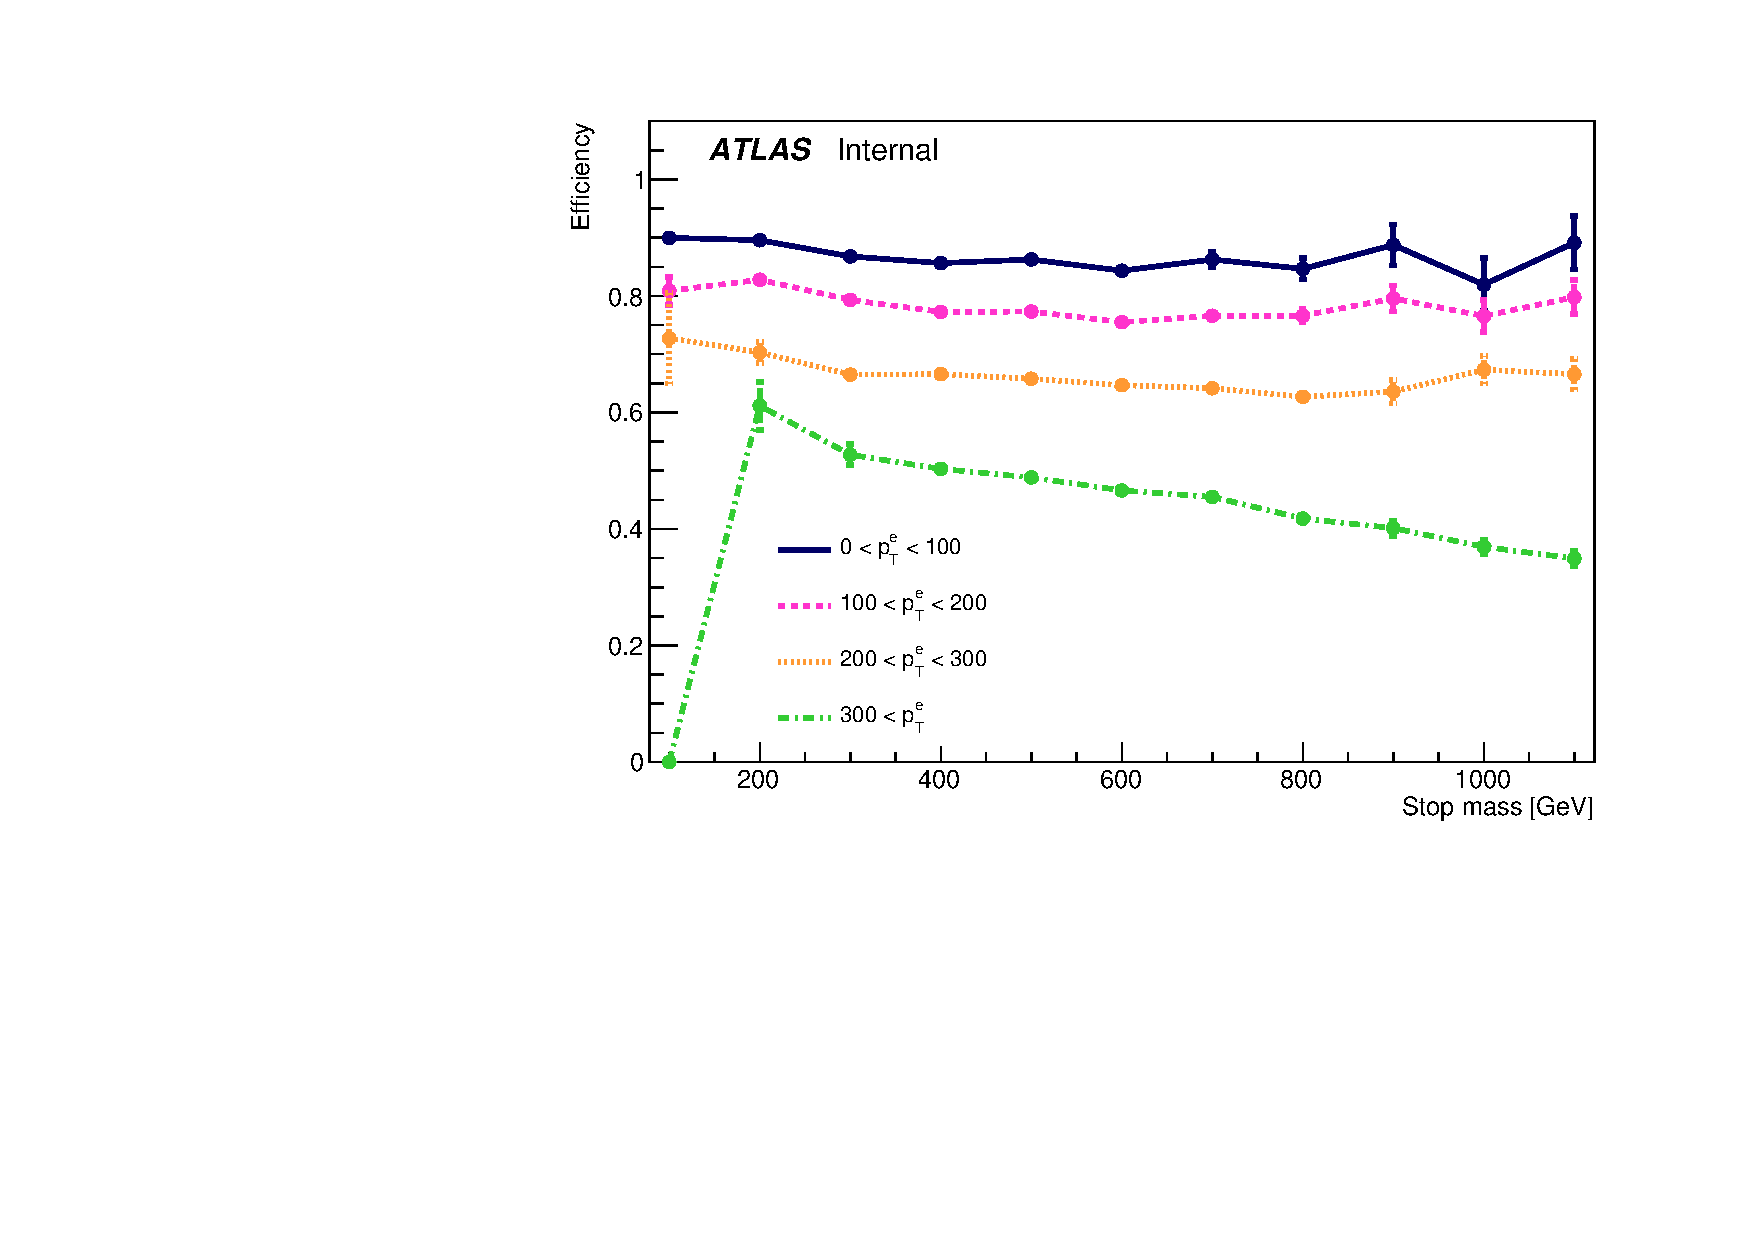
\includegraphics[width=0.48\textwidth, clip=true, trim=0 0 1cm 0]
      {figs/trigger/EF_e24vhi_medium1__el_pt.pdf}
  }
  \subbottom[\texttt{EF\_e60\_medium1}]{
    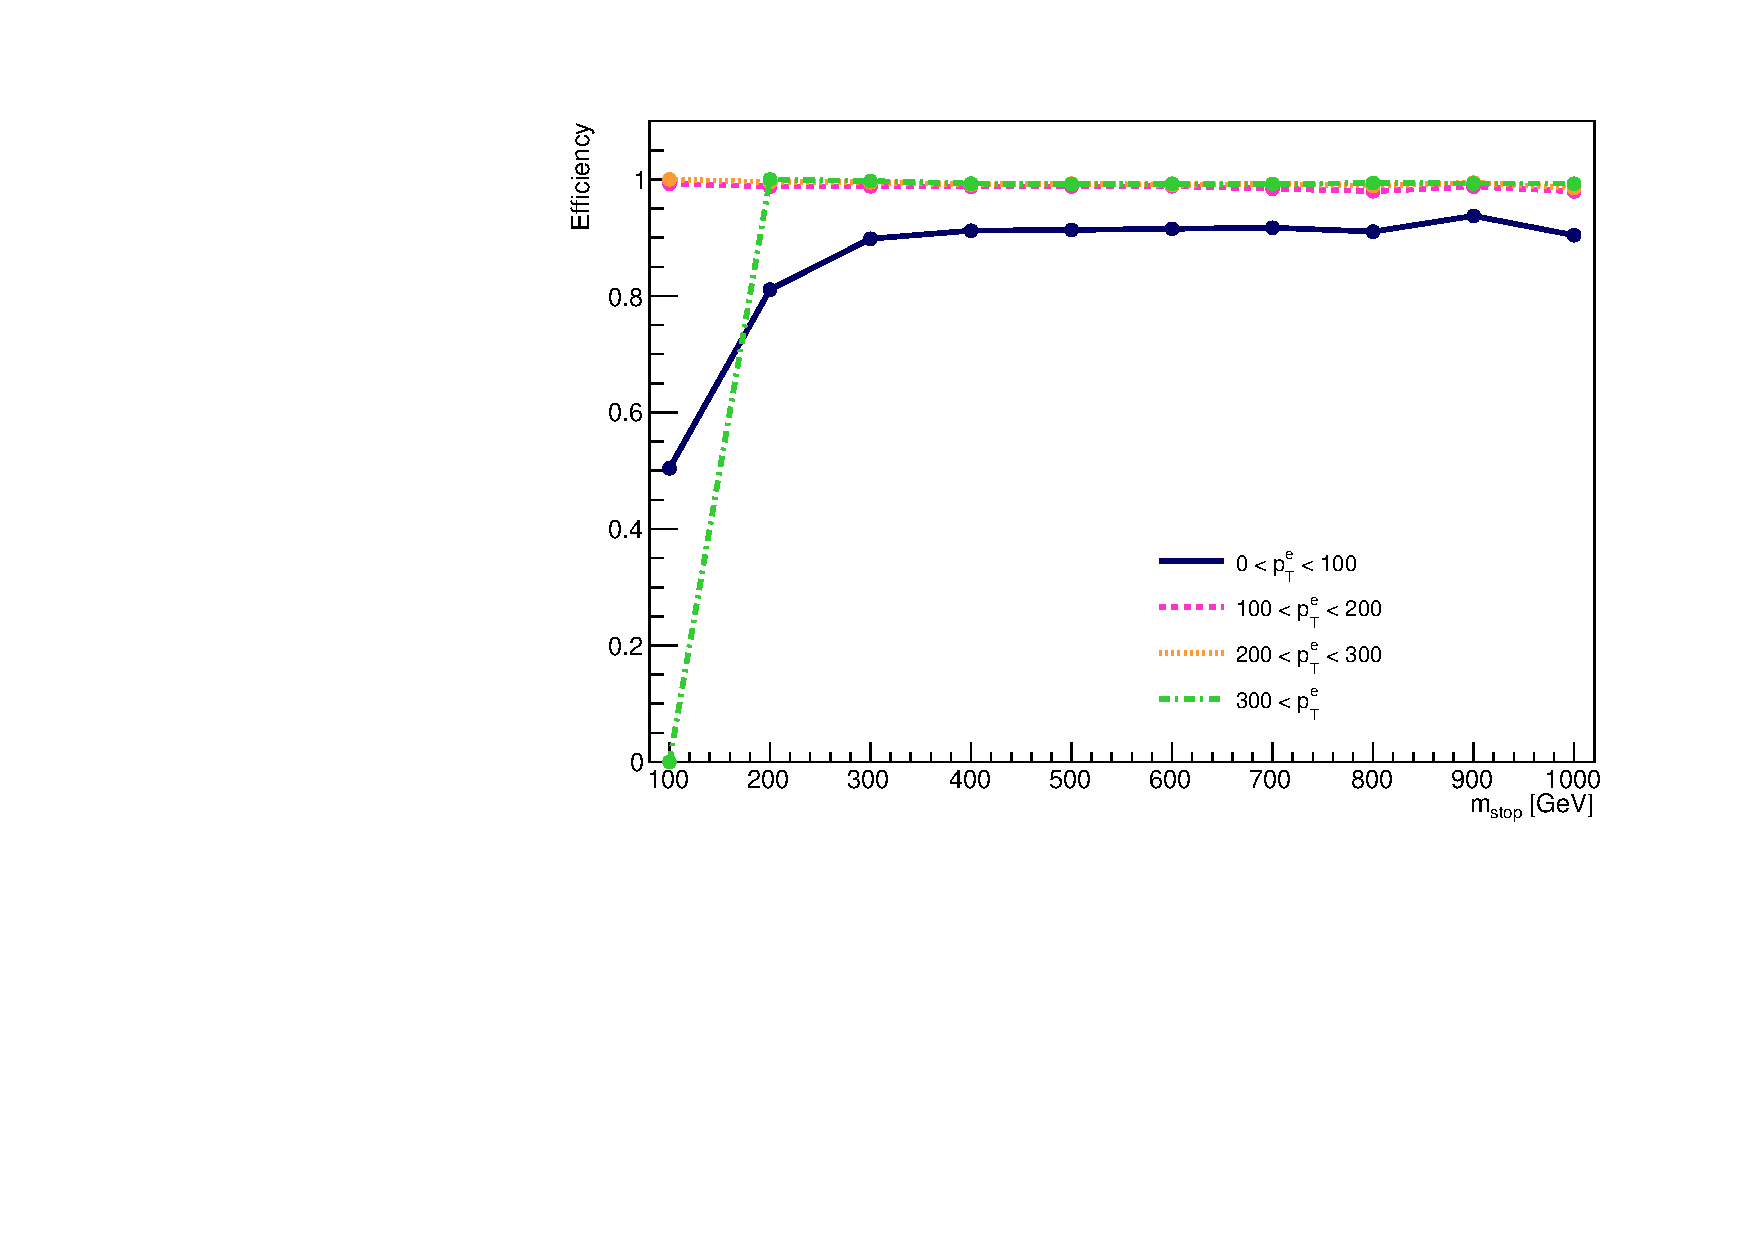
\includegraphics[width=0.48\textwidth, clip=true, trim=0 0 1cm 0]
      {figs/trigger/EF_e60_medium1__el_pt.pdf}
  }
  \caption{Efficiency of simulated stop events passing each of the single
    electron triggers for several ranges of electron \ET.
    Only $e\mu$ events are shown in order to show to isolate the effect of
    the electron \ET\ on the single electron trigger efficiency.
    % These plots show the trigger efficiency dependence on the stop mass,
    % observed in Figure~\ref{fig:single_trigger_efficiency} is due to a
    % dependence on the electron \HT.
    % The \texttt{EF\_e24vhi\_medium1} trigger has the high efficiency for low
    % \HT\ electrons, while the \texttt{EF\_e60\_medium1} trigger is more
    % efficient for high \HT\ electrons.
  }
  \label{fig:electron_trigger_pt_dependence}
\end{figure}

The full trigger requirement is highly efficient for signal-like events; between
93\% and 98\% of simulated signal events pass the trigger selection depending
on the flavor channel as shown in Figure~\ref{fig:full_trigger_efficiency}.

\begin{figure}[ht]
  \centering
  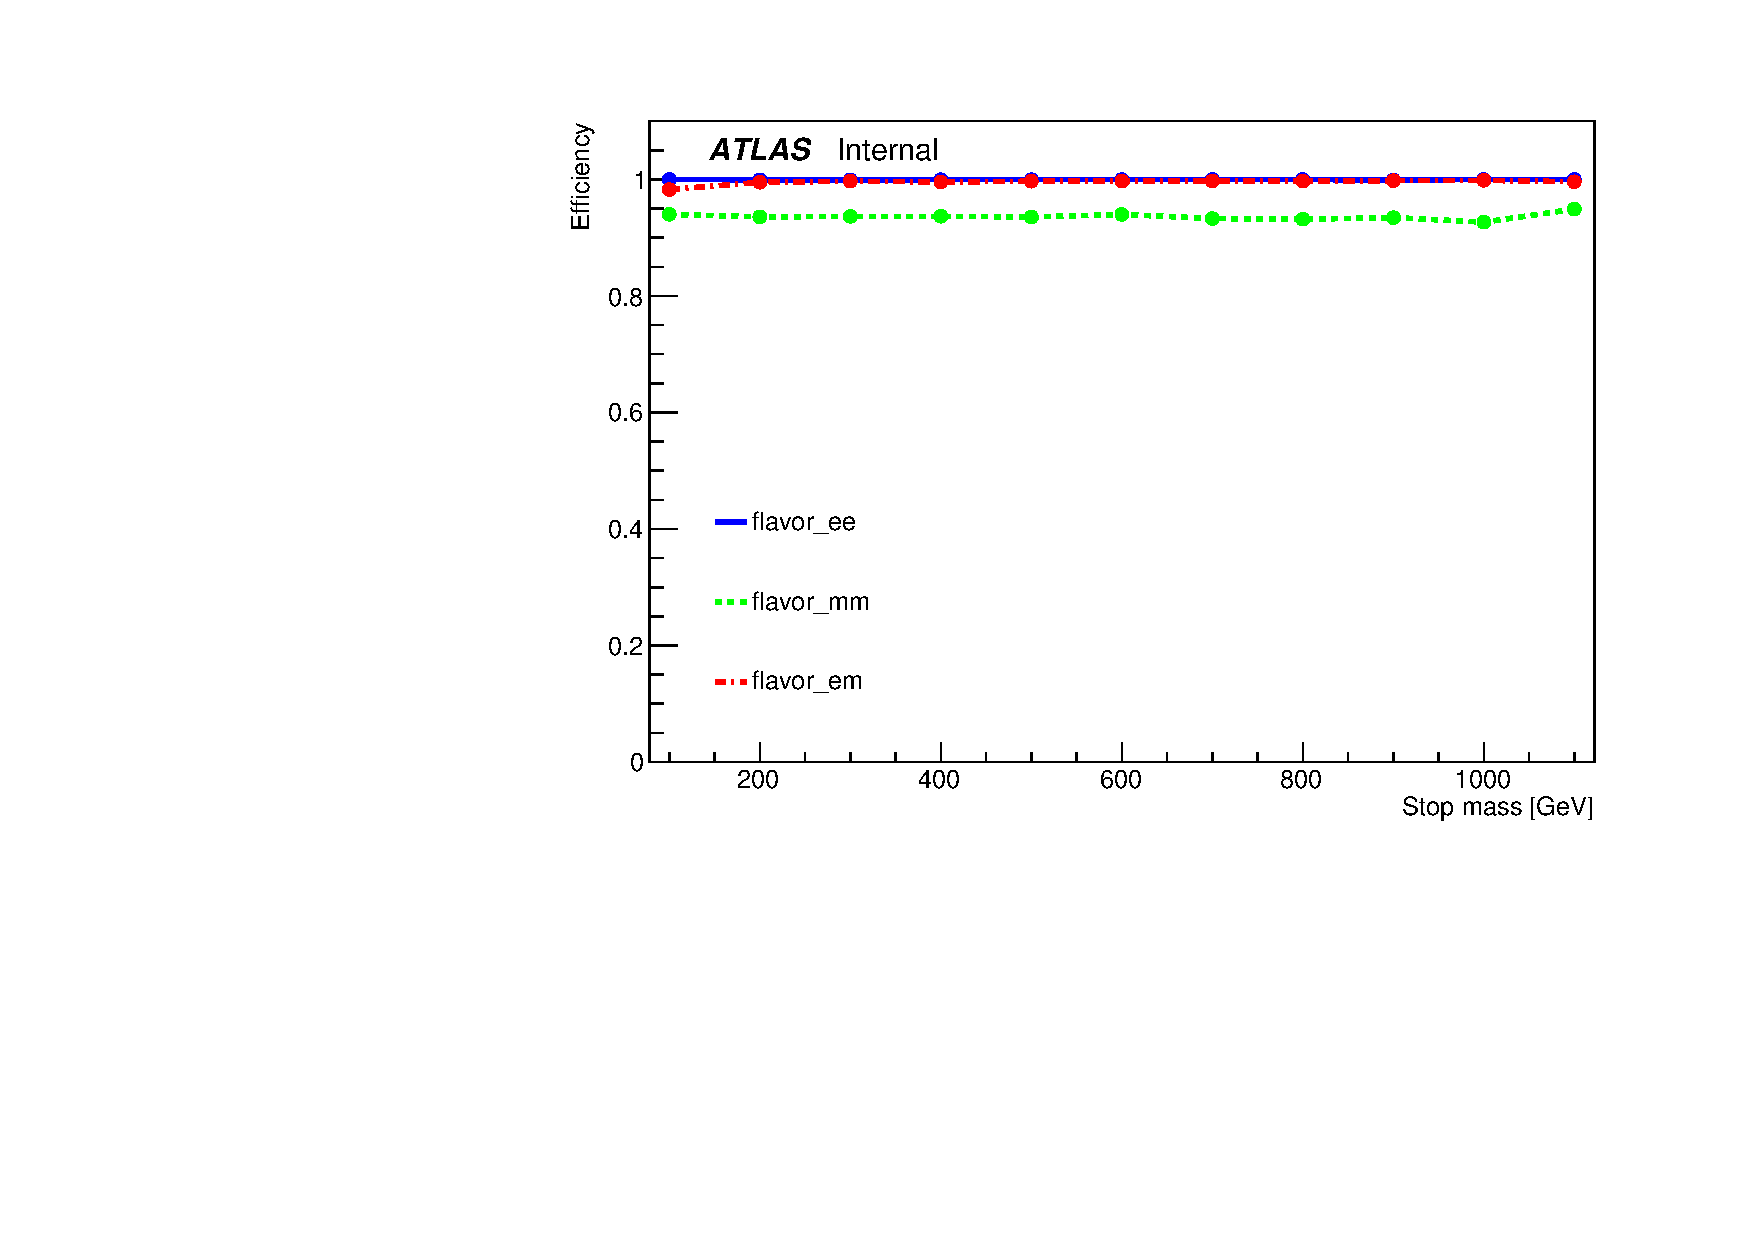
\includegraphics[width=0.75\textwidth]
    {figs/trigger/EF_e24vhi_medium1_OR_EF_e60_medium1_OR_EF_mu24i_tight_OR_EF_mu36_tight.pdf}
  \caption{Efficiency of simulated stop events passing the full trigger
    selection broken down by flavor channel.
    When the full trigger selection is considered, the trigger efficiency does
    not depend on the stop mass.
  }
  \label{fig:full_trigger_efficiency}
\end{figure}

The trigger requirement is applied in both data and MC simulation.
To account for the difference in trigger efficiency, a trigger scale factor is
applied to the MC events passing the trigger requirement.
The trigger efficiencies for data and MC simulation are provided by
the Egamma and Muon combined performance
groups~\cite{ATLAS-CONF-2014-032,Aad:2014rra}.
The trigger scale factor is the ratio (data to MC simulation) of the
efficiencies for an event passing the trigger requirement, described in
Table~\ref{tab:triggers}, and is given by
\begin{equation}
  SF_\mathrm{trigger} =
  \frac{1- \prod_{t \in \mathrm{triggers}}\prod_{\ell \in \{0,1\}}
                 (1-\epsilon_{\ell, t}^\mathrm{data})}
       {1- \prod_{t \in \mathrm{triggers}}\prod_{\ell \in \{0,1\}}
                 (1-\epsilon_{\ell, t}^\mathrm{MC})},
\end{equation}
where $\epsilon_{\ell,t}^\mathrm{data}$ ($\epsilon_{\ell,t}^\mathrm{MC}$) is
the trigger efficiency (electron or muon) for lepton $\ell$ to pass trigger $t$
in the data (MC simulation).
The trigger scale factor is calculated using the two signal leptons in the
event, as these are the only objects considered when checking the trigger
requirement.
The efficiency for an electron (muon) to pass one of the muon (electron)
triggers is set to zero.
This is justified based on the trigger efficiencies shown in
Figure~\ref{fig:single_trigger_efficiency}.
The trigger scale factor is treated as an additional event weight for events in
the MC simulation.

%% -----------------------------------------------------------------------------
\FloatBarrier
\section{Signal regions}
\label{sec:signal_regions}

The goal of this analysis is to define a signal region with low background
contamination in order to search for pair production of massive stops.
As the analysis targets a wide range of stop masses; therefore, the expected
kinematics of the stop decay products have a large range as well.
Two overlapping signal regions (SRs) are defined to search for an excess of
signal-like events, inconsistent with the prediction from the SM alone.
Several kinematic quantities, calculated from the four-vectors of the two
leptons and two $b$-tagged jets provide excellent discrimination to reject
background. 
These quantities are discussed below and shown in
Figure~\ref{fig:no_data__no_k__inclusive_flavor_all__kinematic_dists} for an
region, applying only event cleaning, and requiring two $b$-tagged jets and
two leptons.

The largest SM processes of background events are \ZGAMMAJETS, \TTBAR, and
single top production.
The selection requirements are optimized using MC simulation to achieve a
large signal to background ration in the SRs.
The optimization assumes a stop branching fraction of
$Br(\STOP\rightarrow~be)~=~Br(\STOP\rightarrow~b\mu)~=~0.5$.
The following selection criteria effectively reduces these, and other
(smaller) SM background, while leaving a reasonably high expected signal
efficiency.

\begin{description}
  \item[$\mathbf{\MLL}$] \hfill \\
    The background from \ZGAMMAJETS\ has a narrow resonance in he invariant
    mass of the two leptons ($\mathbf{\MLL}$) around the $Z$~boson mass of
    91~\GeV, as seen in
    Figure~\ref{fig:no_data__no_k__inclusive_flavor_all__kinematic_dists}.
    Events with two leptons of the same flavor ($ee$ or $\mu\mu$), with a
    reconstructed invariant mass consistent with the $Z$~boson
    ($|m_{\ell\ell} - m_{Z}| \leq 10 \GeV$) are rejected to reduce the
    contributions of the \ZGAMMAJETS\ background.
  %%
  \item[$\mathbf{\HT}$] \hfill \\
    The leptons and $b$-jets from the two-body decays of massive stops tend to
    have more \pt\ than those from the decays of lower mas SM particles.
    The $\mathbf{\HT}$\ variable, shown in
    Figure~\ref{fig:no_data__no_k__inclusive_flavor_all__kinematic_dists},
    is the scalar sum of the \et(\pt) of the two $b$-tagged jets and the two
    leptons.
    Events in the SRs are required to have $\HT \geq 1100 \GeV$.
  %%
  \item[$\mathbf{\MBL^{0}}$] \hfill \\
    The invariant masses of he two $b\ell$ pairs provide two ways to reduce
    the background from SM processes.
    Firstly, the highest invariant mass value, $\mathbf{\MBL^{0}}$, has a broad
    resonance about the stop mass, as seen in
    Figure~\ref{fig:no_data__no_k__inclusive_flavor_all__kinematic_dists},
    while the SM backgrounds have lower values.
    Since a large range of stop masses are considered, two overlapping SRs are
    defined, differing in the \MBL-requirement.
    SR~400 is optimal for lower stop masses, and has a requirement of
    $\MBL^0 \geq 400~\GeV$, while SR~600, with a requirement of
    $\MBL^0 \geq 600 \GeV$, is optimal for higher stop masses.
    \\[1ex]
    Two additional SRs were considered with $\MBL^0 \geq 200 \GeV$ and
    $\MBL^0 \geq 800 \GeV$ (SR~200 and SR~800 respectively), however these
    were dropped from the analysis.
    The SR~200 region did not provide additional expected sensitivity compared
    with the SR~400 region, and the statistical uncertainty in the SR~800
    region was very large, and reduced expected sensitivity.
  %% 
  \item[$\mathbf{\MBL}$~\textbf{asymmetry}] \hfill \\
    Secondly, event when $\MBL^{0}$ is large, the difference in invariant mass
    between the highest and lowest pair can be large for SM processes as seen
    in 
    Figure~\ref{fig:no_data__no_k__inclusive_flavor_all__kinematic_dists}.
    To quantify the difference in the two masses, the
    $\mathbf{\MBL}$~\textbf{asymmetry} is defined as
    $\MBLASYM = \nicefrac{\MBL^0-\MBL^1}{\MBL^0+\MBL^1}$.
    The \MBLASYM\ is used rather than the simple difference in the masses
    because it is incorporates the effects of the mass scale, and as single
    requirement on the \MBLASYM\ can be used for all stop masses which are
    considered.
    In order to be selected for one or both of the SRs, an event requires
    $\MBLASYM \leq 0.2$.
  %%
\end{description}

% The scalar sum of the \et(pt) of the two $b$-tagged jets and two leptons (\HT) 
% effectively separates the signal processes from the major sources of
% Standard Model background.
% The stops of interest are extremely massive, so all the decay products tend to
% have a large amount of energy, resulting in a high \HT.
% SM processes, such as \TTBAR\ and \ZGAMMAJETS, do not have as large \HT.

% For the signal model, the two $b\ell$ pairs making up the final state are the
% decay products of the stop/anti-stop, and therefore have the same mass.
% The mass asymmetry variable is defined as
% \begin{equation}
%   \MBLASYM = 
%   \frac{\MBL^0-\MBL^1}{\MBL^0+\MBL^1}.
% \end{equation}
% Events from stop decays are expected to have low \MBLASYM\ as the mass
% difference in the two pairs is expected to be small, while the masses of the
% $b\ell$ pairs coming from SM processes are roughly uncorrelated, and there is
% no preference for \MBLASYM.
% The asymmetry is used rather than the simple difference in the masses to remove
% the effect of the mass scale, and a single cut value can be used for all stop
% masses which are considered.
% Events from SM background processes tend to have low \MBL\ for
% both pairs.
% The $\MBL^0$ variable can also provide additional discrimination power.
% The expected \MLL, \HT, \MBLASYM\, and $\MBL^{0}$ distributions for SM
% background processes and three signal models is shown in an inclusive region
% after event cleaning and selecting two $b$-tagged jets and two leptons in
% Figure~\ref{fig:no_data__no_k__inclusive_flavor_all__kinematic_dists}.

\begin{figure}
  \centering
  \subbottom[\MLL]{
    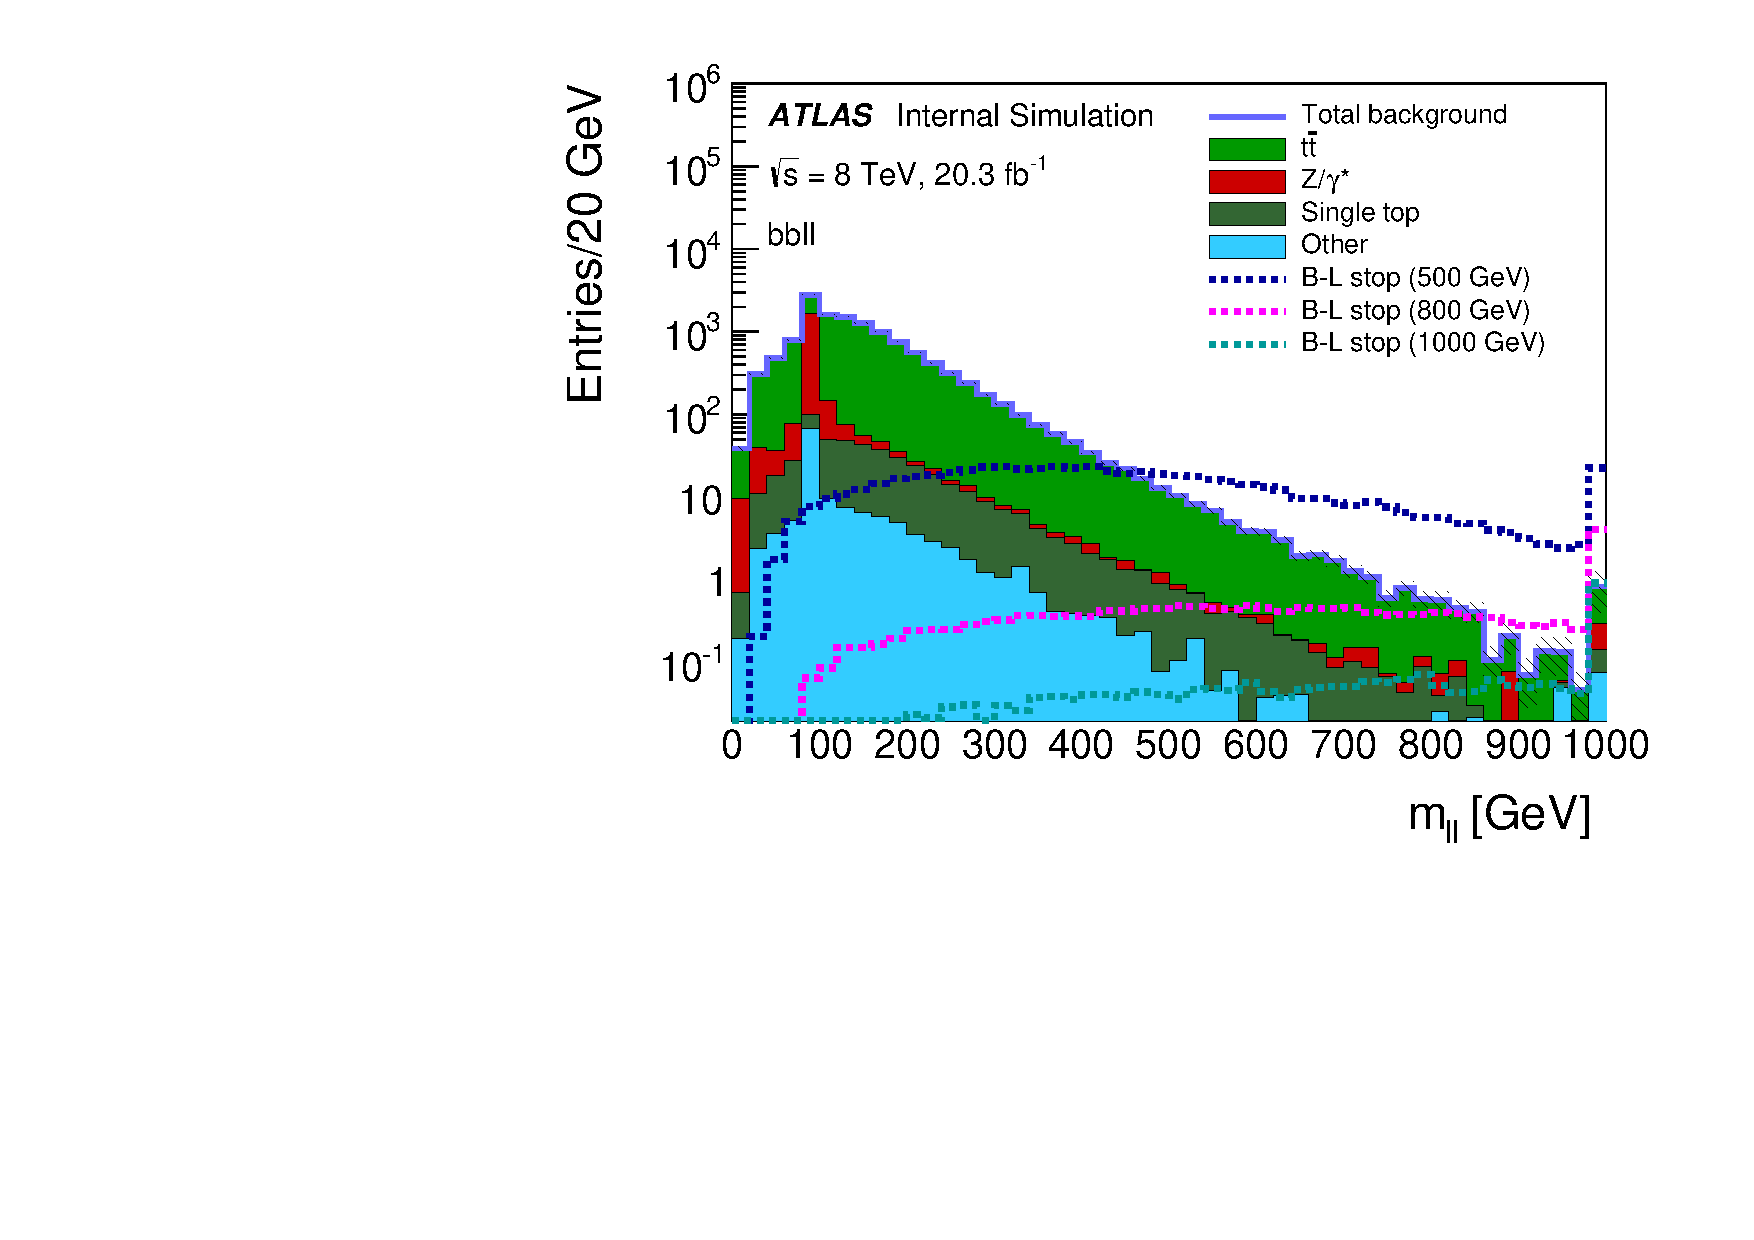
\includegraphics[width=0.48\textwidth, clip=true, trim=0 0 1cm 0]
    {figs/blstop/no_data__no_k_factor__dists/flavor_all__mll__BMINUSL_BL_PAIRING__log.pdf}
  }
  \subbottom[\HT]{
    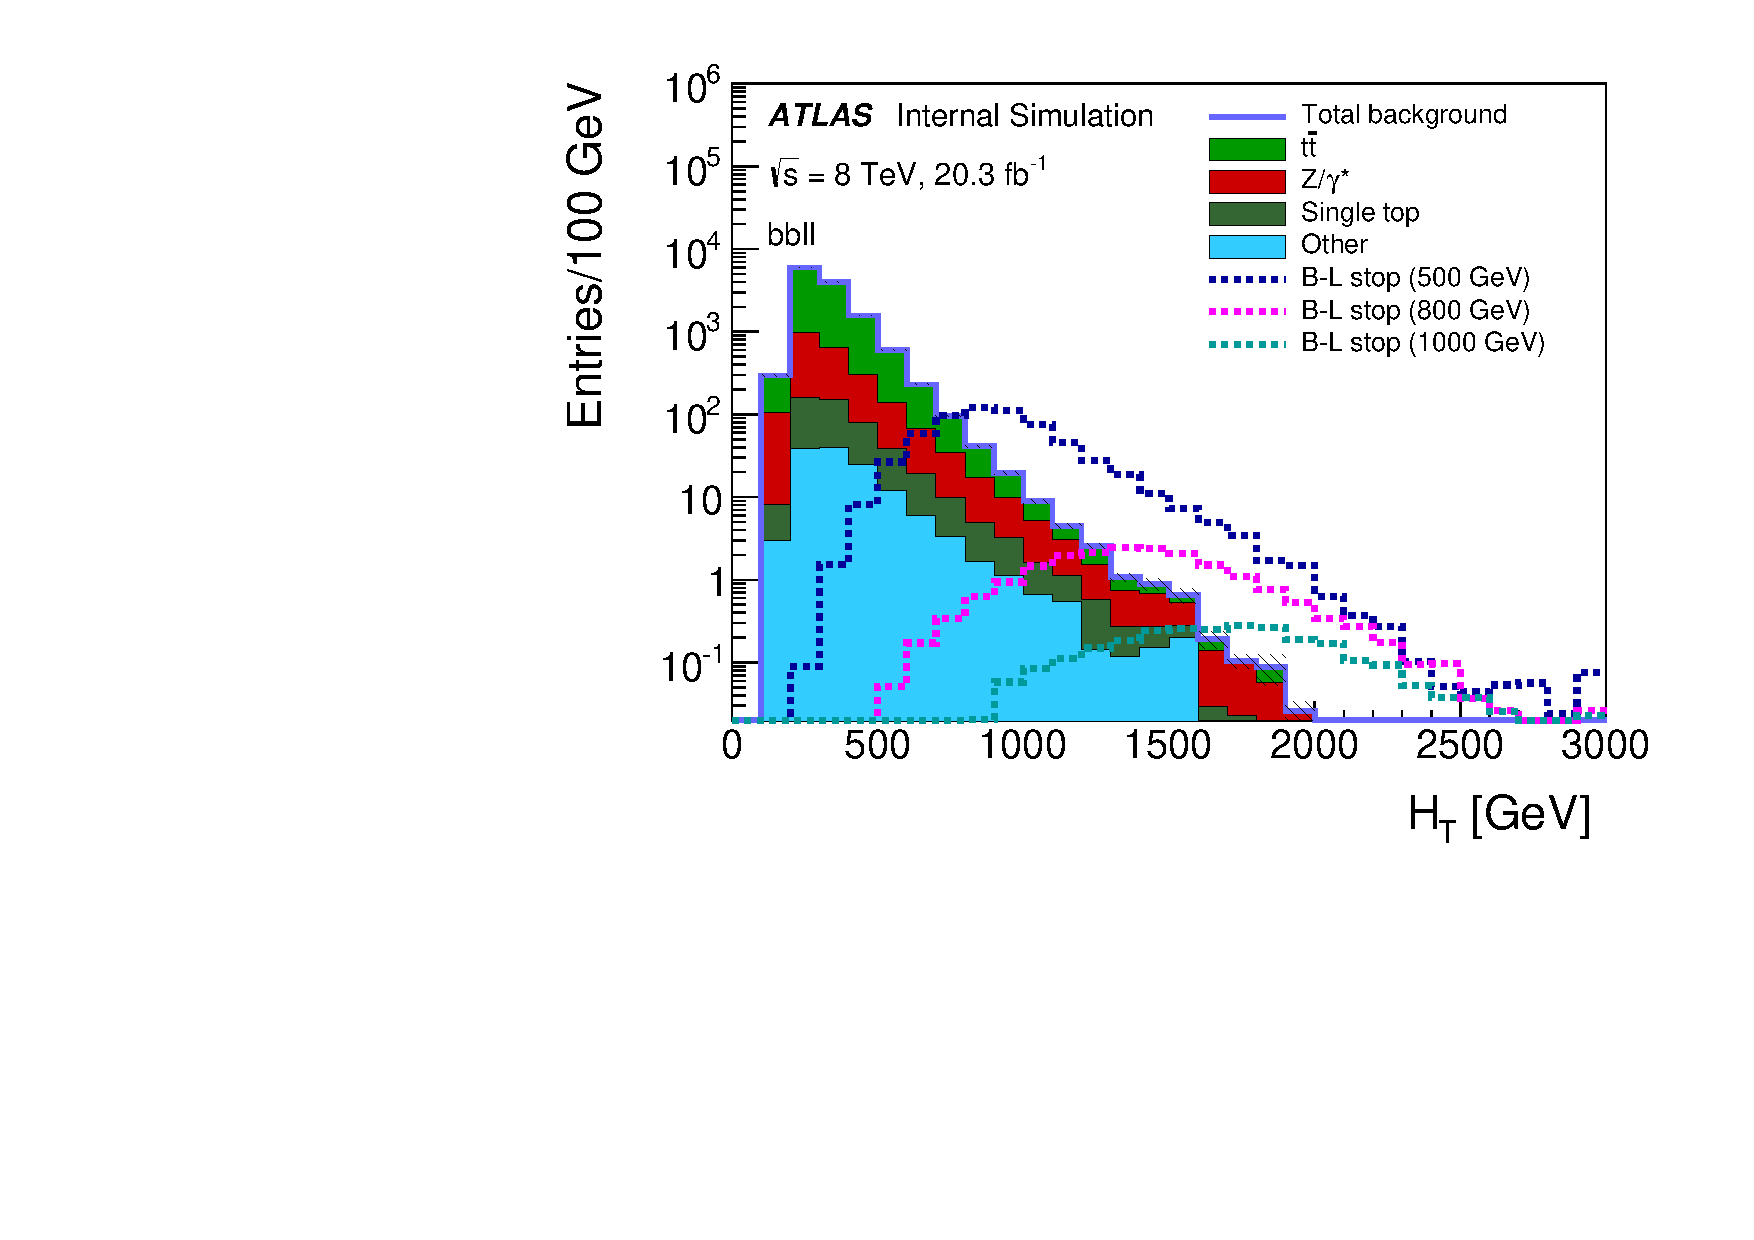
\includegraphics[width=0.48\textwidth, clip=true, trim=0 0 1cm 0]
    {figs/blstop/no_data__no_k_factor__dists/flavor_all__ht_signal__BMINUSL_BL_PAIRING__log.pdf}
  }
  \subbottom[\MBLASYM]{
    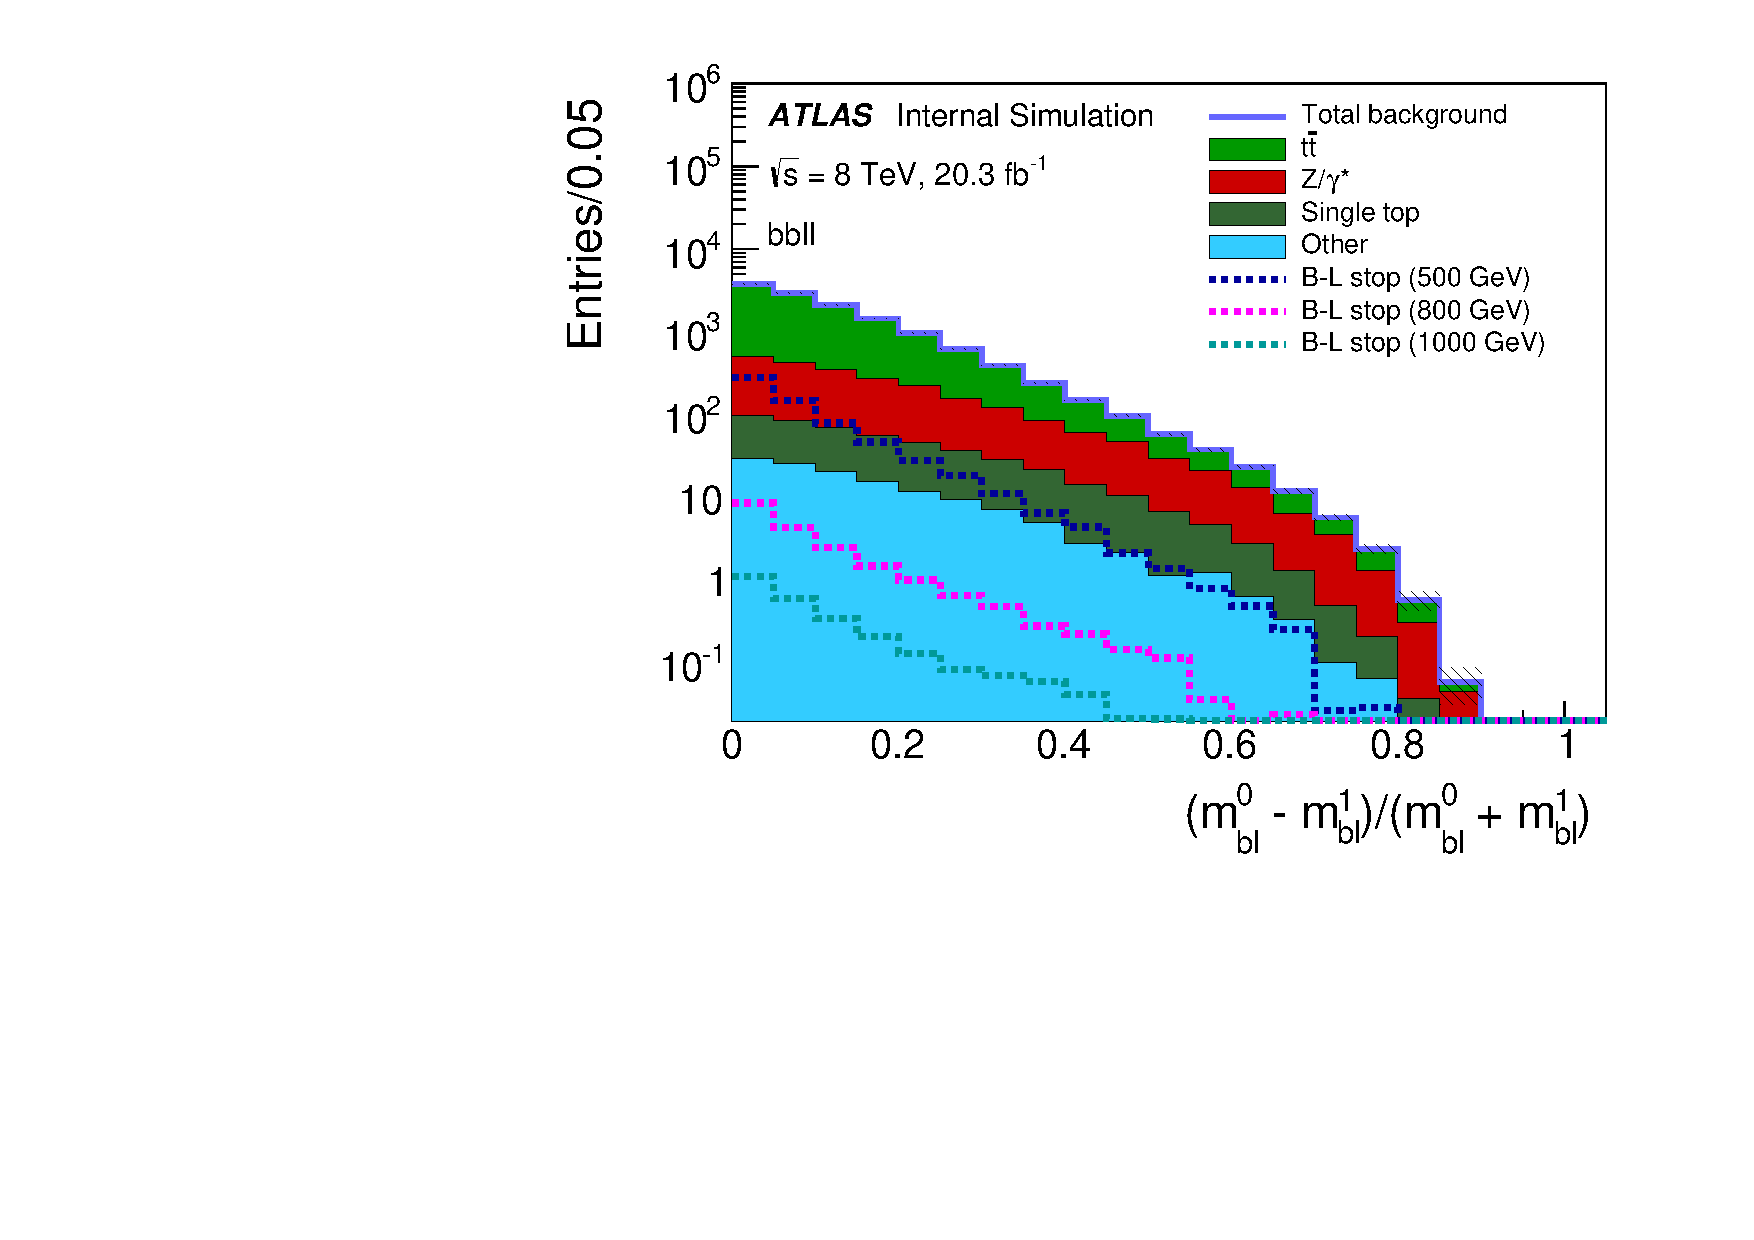
\includegraphics[width=0.48\textwidth, clip=true, trim=0 0 1cm 0]
    {figs/blstop/no_data__no_k_factor__dists/flavor_all__mbl_asym__BMINUSL_BL_PAIRING__log.pdf}
  }
  \subbottom[$\MBL^0$]{
    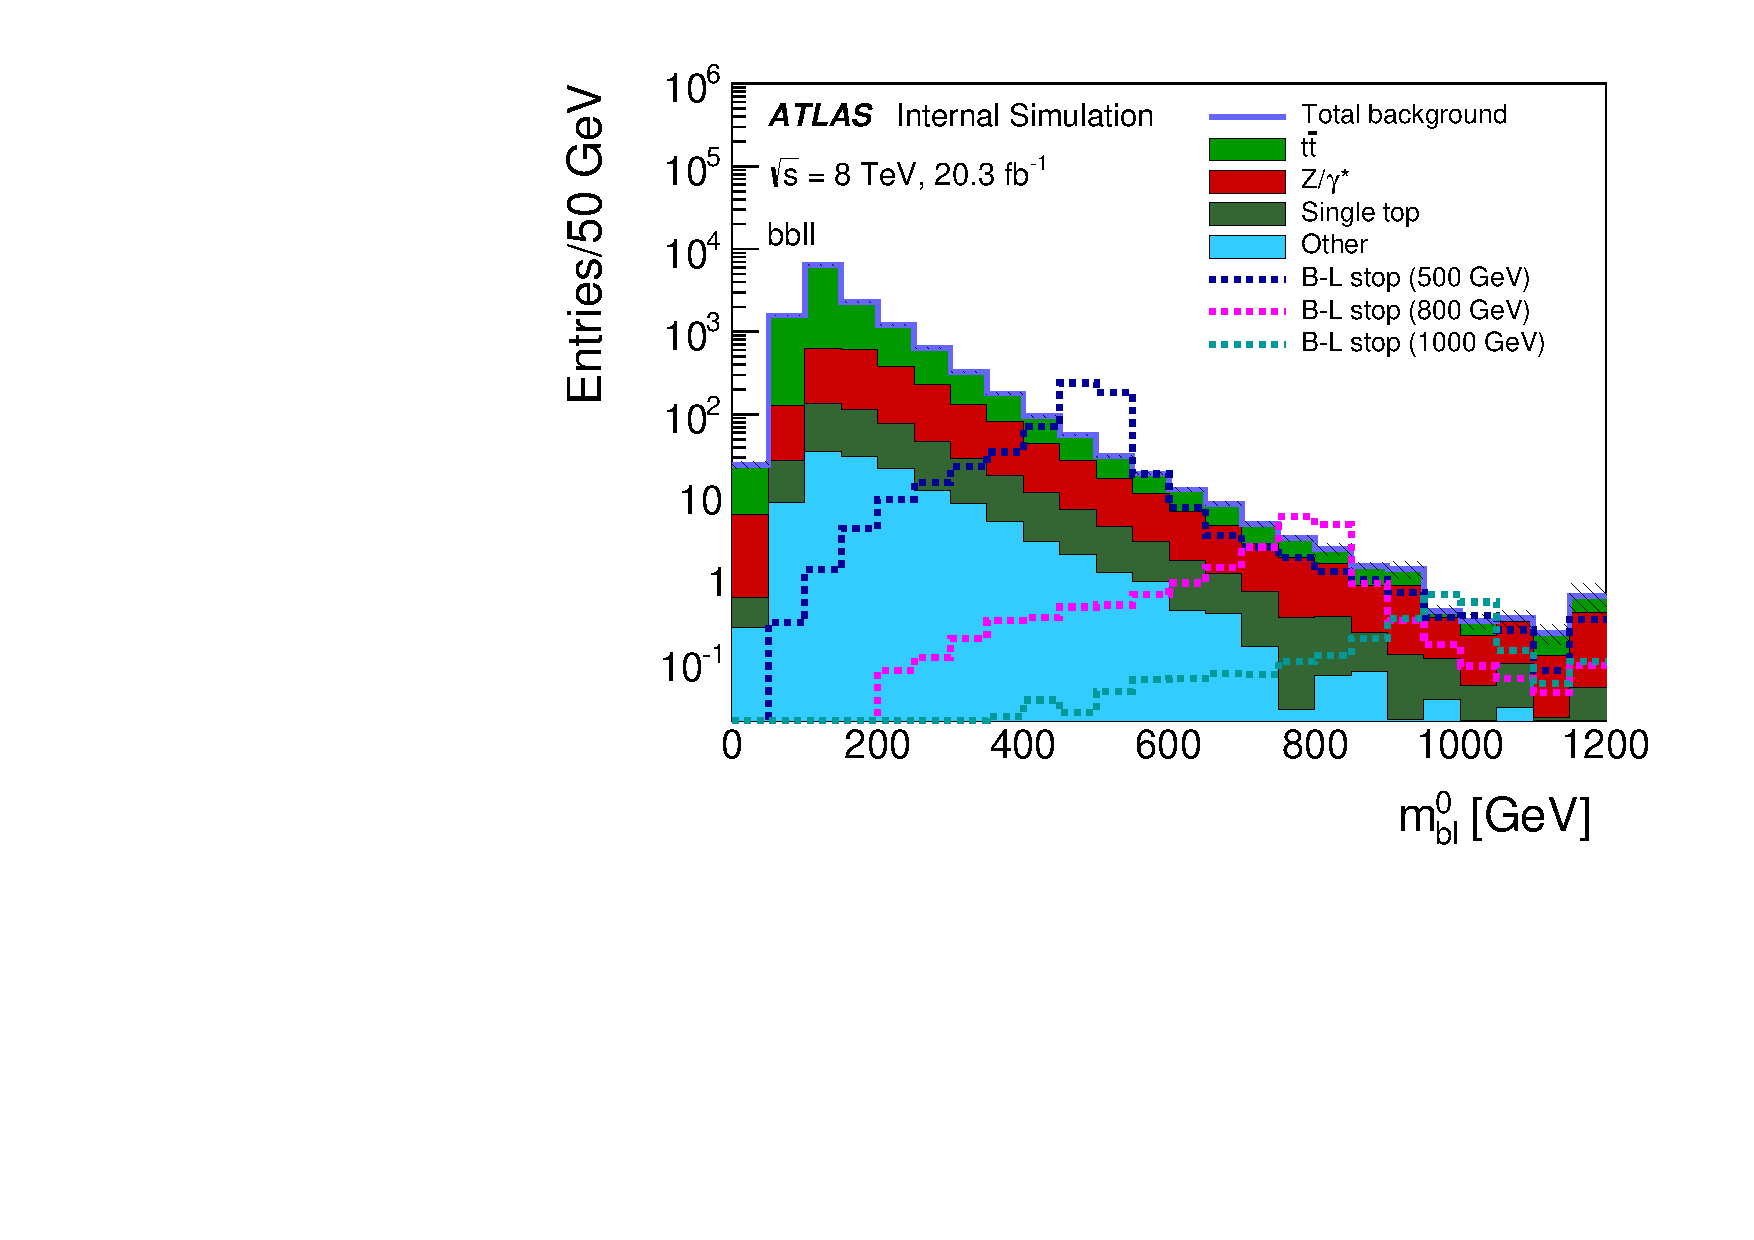
\includegraphics[width=0.48\textwidth, clip=true, trim=0 0 1cm 0]
    {figs/blstop/no_data__no_k_factor__dists/flavor_all__mbl_0__BMINUSL_BL_PAIRING__log.pdf}
  }
  \caption{Expected \MLL, \HT, \MBLASYM, and $\MBL^0$ distributions for SM
    background processes and three simulated stop samples with different masses.
    Basic event cleaning is applied and the events are required to pass the
    trigger selection, as described in
    Sections~\ref{sec:event_cleaning}~and~\ref{sec:trigger_selection}, and the
    events are required to have at least two $b$-tagged jets and two light
    leptons (electrons or muons).
    In each plot, the last bin includes the overflow for values beyond the
    maximum shown. The hashed error bands show only the statistical
    uncertainty in the background MC simulation samples. The signal
    models have an assumed
    $Br(\STOP\rightarrow~be)~=~Br(\STOP\rightarrow~b\mu)~=~0.5$.
  }
  \label{fig:no_data__no_k__inclusive_flavor_all__kinematic_dists}
  %%
\end{figure}

%% MC simulation is used to optimize the selection requirements and achieve a
%% large signal to background ration in the SRs.
%% The optimization is performed assuming a stop branching fraction of
%% $Br(\STOP\rightarrow~be)~=~Br(\STOP\rightarrow~b\mu)~=~0.5$.
%% A single SR selection criteria is obtained for both the \HT\ and
%% \MBLASYM\ variables which perform reasonably well for all mass above 400~\GeV.
%% Events in both SRs are required to have $\HT \geq 1100\,\GeV$ and
%% $\MBLASYM \leq 0.2$.
%% Events with two same flavor leptons with invariant mass within 10~\GeV\ of the
%% $Z$-boson mass are vetoed to reduce the backgrounds from $Z$-boson production.
%% $\MBL^0$ is used to define the two SRs.
%% SR~400 has a requirement of $\MBL^0 \geq 400~\GeV$, and is optimal for lower
%% stop masses, while SR~600, with a requirement of $\MBL^0 \geq 600 \GeV$, is
%% optimal for higher stop masses.
%% 
%% Two additional SRs were considered with $\MBL^0 \geq 200 \GeV$ and
%% $\MBL^0 \geq 800 \GeV$ (SR~200 and SR~800 respectively), however these were
%% dropped from the analysis.
%% The SR~200 region did not provide additional expected sensitivity compared with
%% the SR~400 region, and the statistical uncertainty in the SR~800 region was very
%% large, and reduced expected sensitivity.
%% % The full selection criteria for the analysis regions, including the Control and
%% % Validation regions, described in Section~\ref{sec:bkg}, is outlined in
%% % Table~\ref{tab:regions} and Figure~\ref{fig:region_coverage}.
%% % 
% %% - - - - - - - - - - - - - - - - - - - - - - - - - - - - - - - - - - - - - - -
% \begin{table}[ht]
%   \caption{Summary of signal, control, and validation regions used for this
%     analysis.
%     The control and validation regions are explained in Section~\ref{sec:bkg}.
%     All regions require two $b$-tagged jets and two oppositely charged leptons.
%     An event is in the $Z$ window if it contains two same-flavored leptons with
%     an invariant mass within 10~\GeV\ of the mass of the $Z$ boson.
%   }
%   \label{tab:regions}
%   %
%   \centering{
%     \begin{tabular}{l|ccccc}
%       \toprule
%       Region &
%       $\MBL^0$ [\GeV] &
%       \HT [\GeV] &
%       \METSIG\ [$\GeV^{1/2}$] &
%       \MBLASYM &
%       $Z$ window \\
%       \midrule
%       SR~400   & $\geq 400$  & $\geq 1100$ & --       & $\leq 0.2$ & Veto   \\[1ex]
%       SR~600   & $\geq 600$  & $\geq 1100$ & --       & $\leq 0.2$ & Veto   \\
%       \midrule
%       Top CR   & $\geq 200$  & $\leq 500$  & $\geq 4$ & $\leq 0.2$ & Veto   \\[1ex]
%       $Z$ CR   & $\geq 200$  & $\leq 500$  & $\leq 4$ & $\leq 0.2$ & Select \\
%       \midrule
%       Top VR 1 & $\geq 200$  & $\leq 500$  & $< 4$    & $\leq 0.2$ & Veto   \\[1ex]
%       Top VR 2 & $\geq 200$  & $\leq 500$  & -        & $>    0.2$ & Veto   \\[1ex]
%       Top VR 3 & $\geq 200$  & $>   500$   & $> 4$    & $>    0.2$ & Veto   \\[1ex]
%       $Z$ VR   & $\geq 200$  & $>   500$   & --       & $\leq 0.2$ & Select \\
%       \bottomrule
%     \end{tabular}
%   }
% \end{table}
% 
% %% - - - - - - - - - - - - - - - - - - - - - - - - - - - - - - - - - - - - - - -
% \begin{figure}[ht]
%   \centering
%   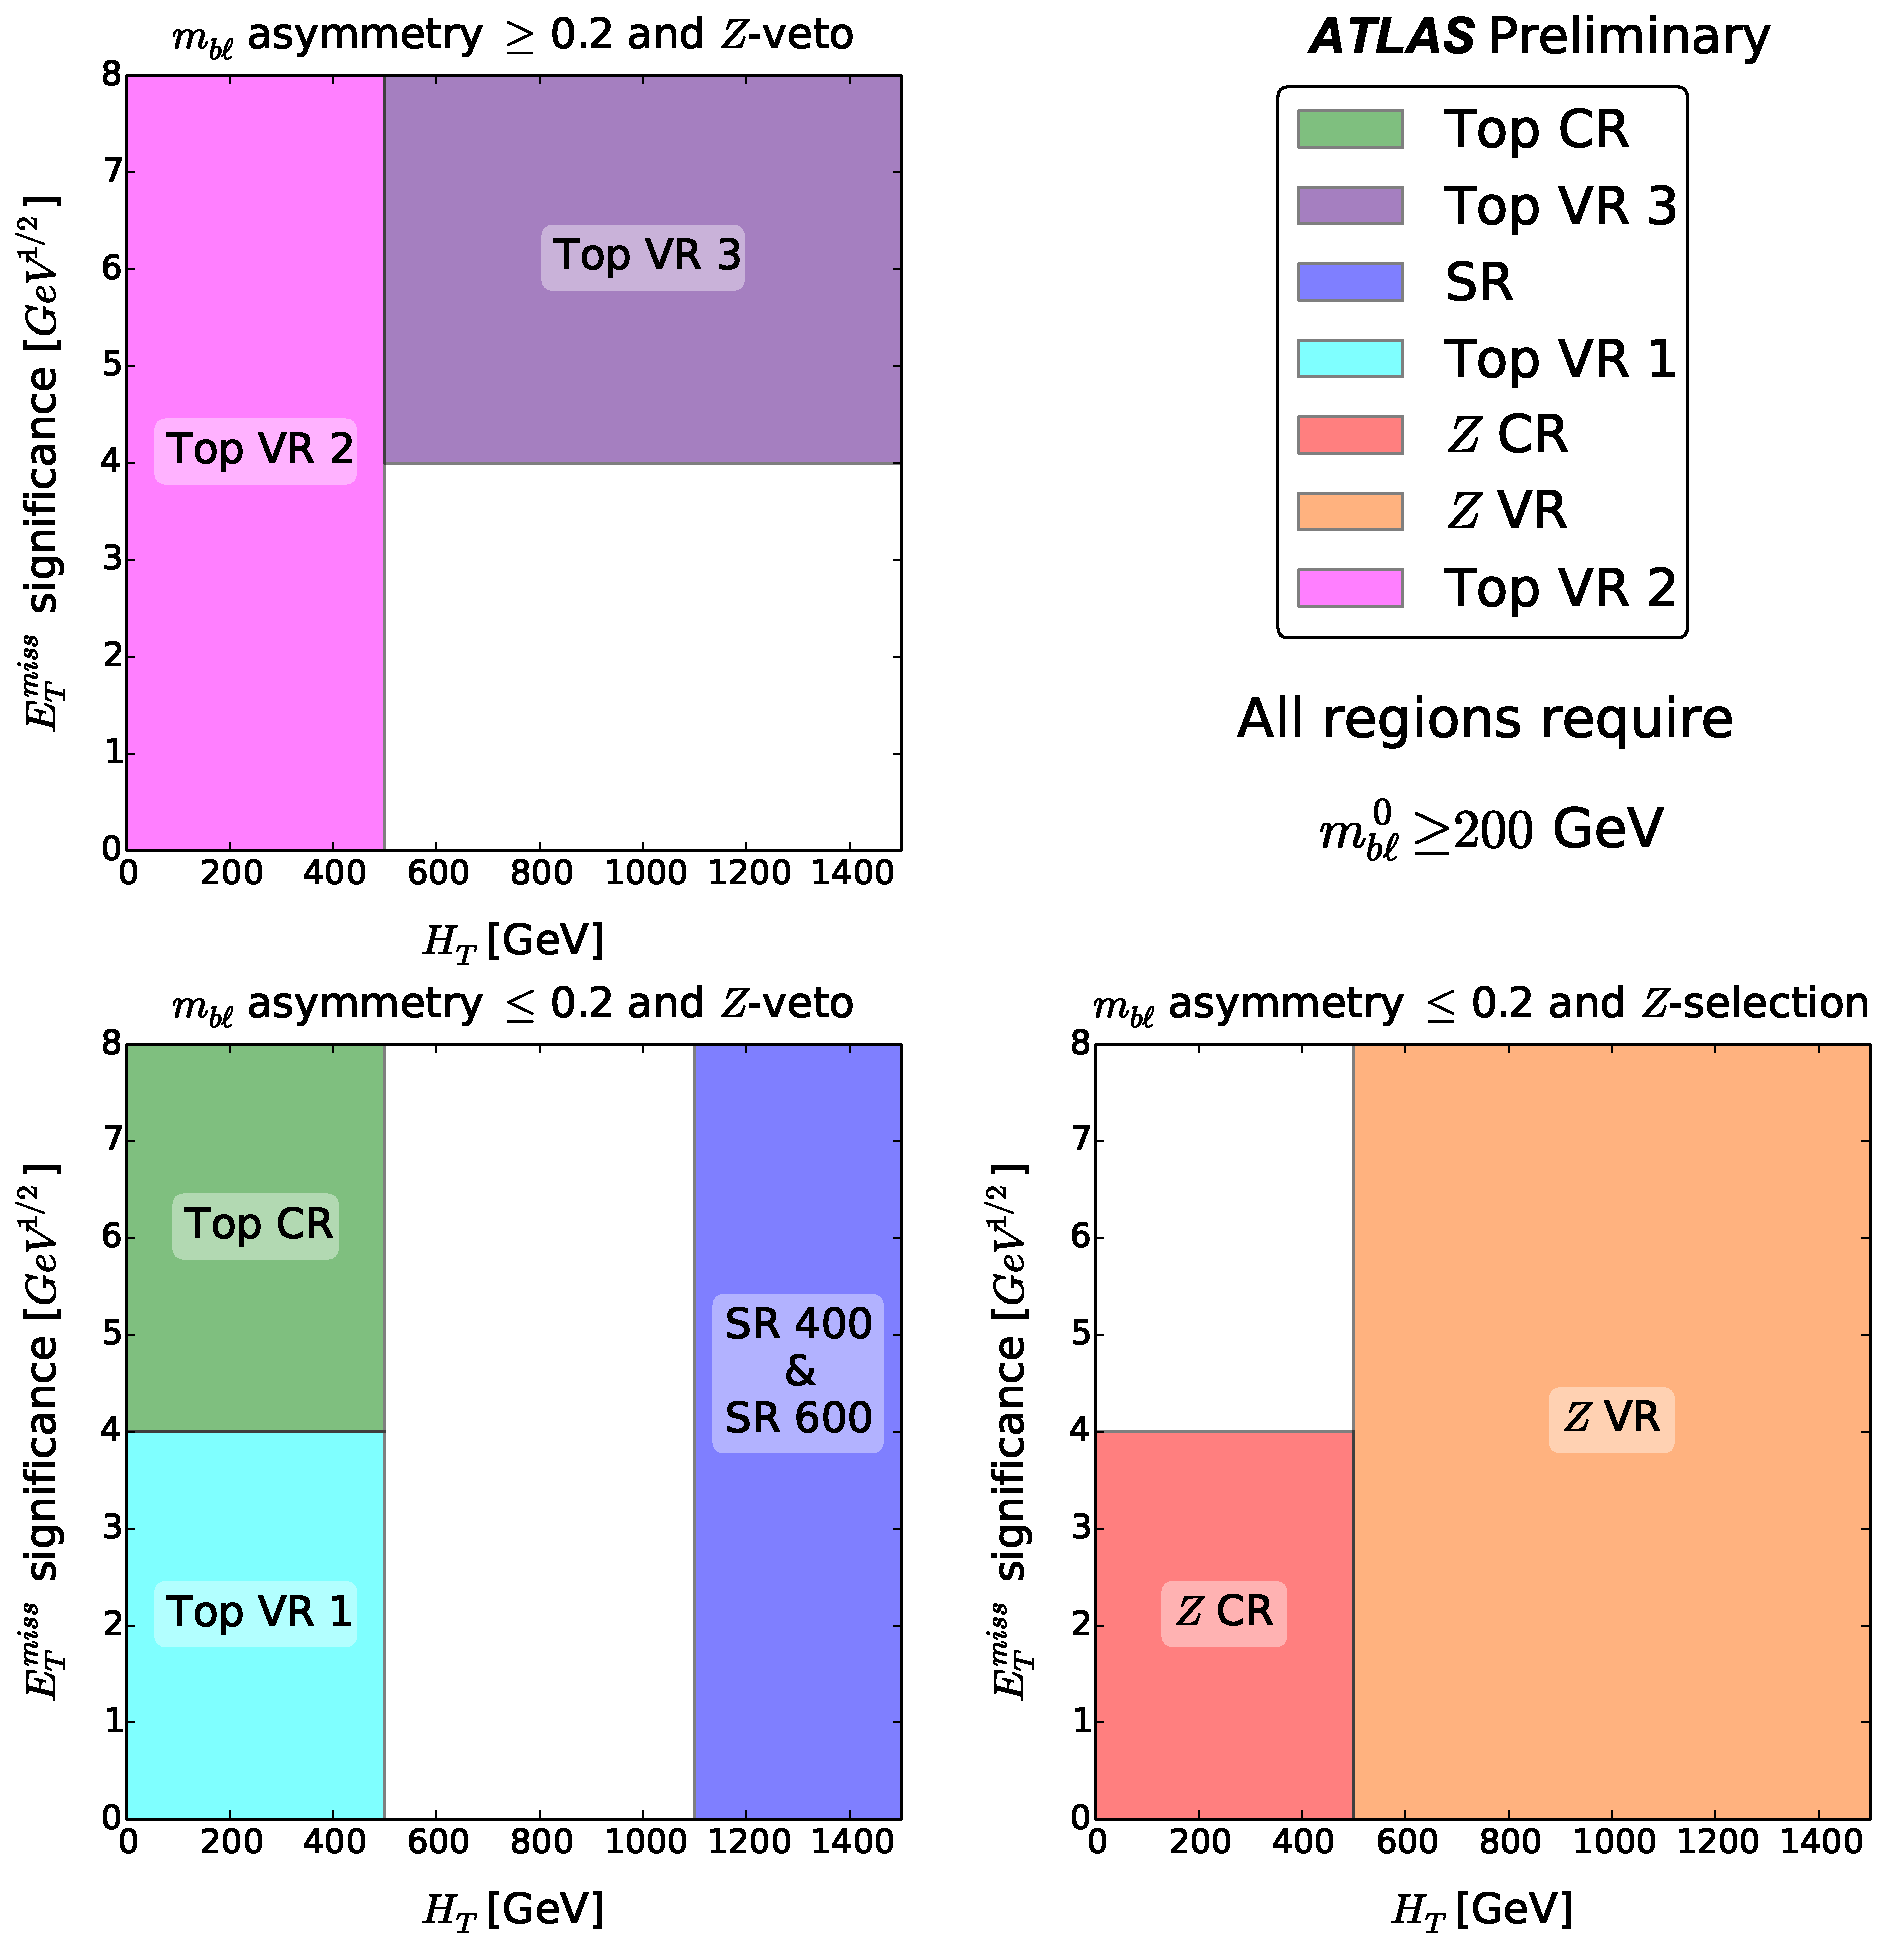
\includegraphics[width=\textwidth]{figs/blstop/regions__met_sig__ht_plane.pdf}
%   \caption{Position of the regions in the \METSIG\ versus \HT\ space.
%     The two left plots show the \METSIG-\HT~plane after vetoing events within
%     the $Z$ window, with the top plot requiring $\MBLASYM \geq 0.2$ and the
%     bottom requiring $\MBLASYM \leq 0.2$.
%     The right plot shows the plane when requiring events be within the $Z$
%     window.
%     The two SRs apply a different requirement on the
%     invariant mass of the higher-mass $b\ell$ pair. SR~400 requires
%     $\MBL^{0} \geq 400 \GeV$, and SR~600 requires $\MBL^{0} \geq 600 \GeV$.
%   }
%   \label{fig:region_coverage}
% \end{figure}

Figure~\ref{fig:n_minus_one_sr} shows the expected \HT, \MBLASYM, and $\MBL^0$
distributions after applying all the SR selection criteria except that on the
variable being shown.
This figure includes the simulated background processes and three signal models.
The number of expected signal events (for the same three signal models)
passing each selection requirement is shown in Table~\ref{tab:sr_cutflow}.
The estimates shown in Figure~\ref{fig:n_minus_one_sr} and
Table~\ref{tab:sr_cutflow} are taken from MC simulation, and the event
yields are normalized to 20.3 \ifb.

\begin{figure}
  \centering
  \subbottom[\HT]{
    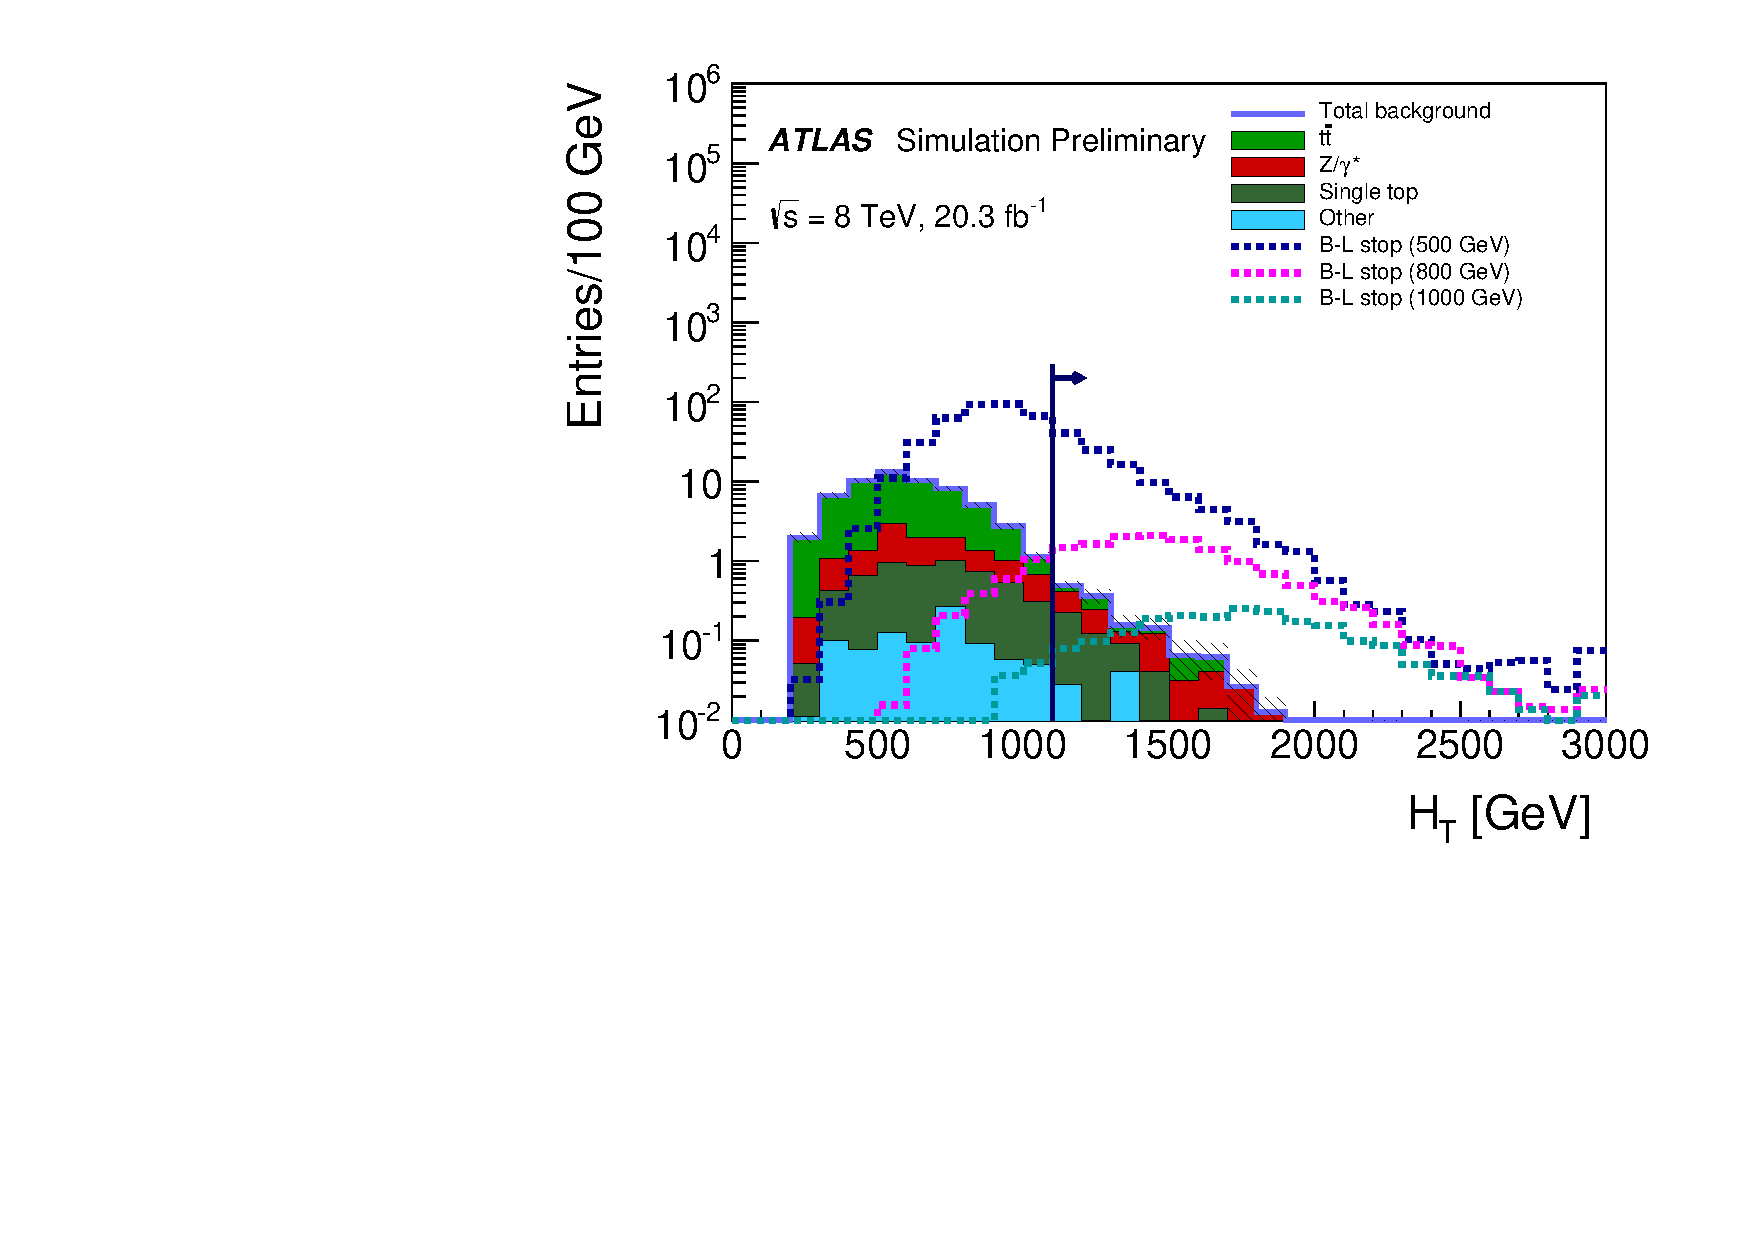
\includegraphics[width=0.48\textwidth, clip=true, trim=0 0 1cm 0]
      {figs/blstop/ht_sr_400_minus_ht.pdf}
  }
  \subbottom[\MBLASYM]{
    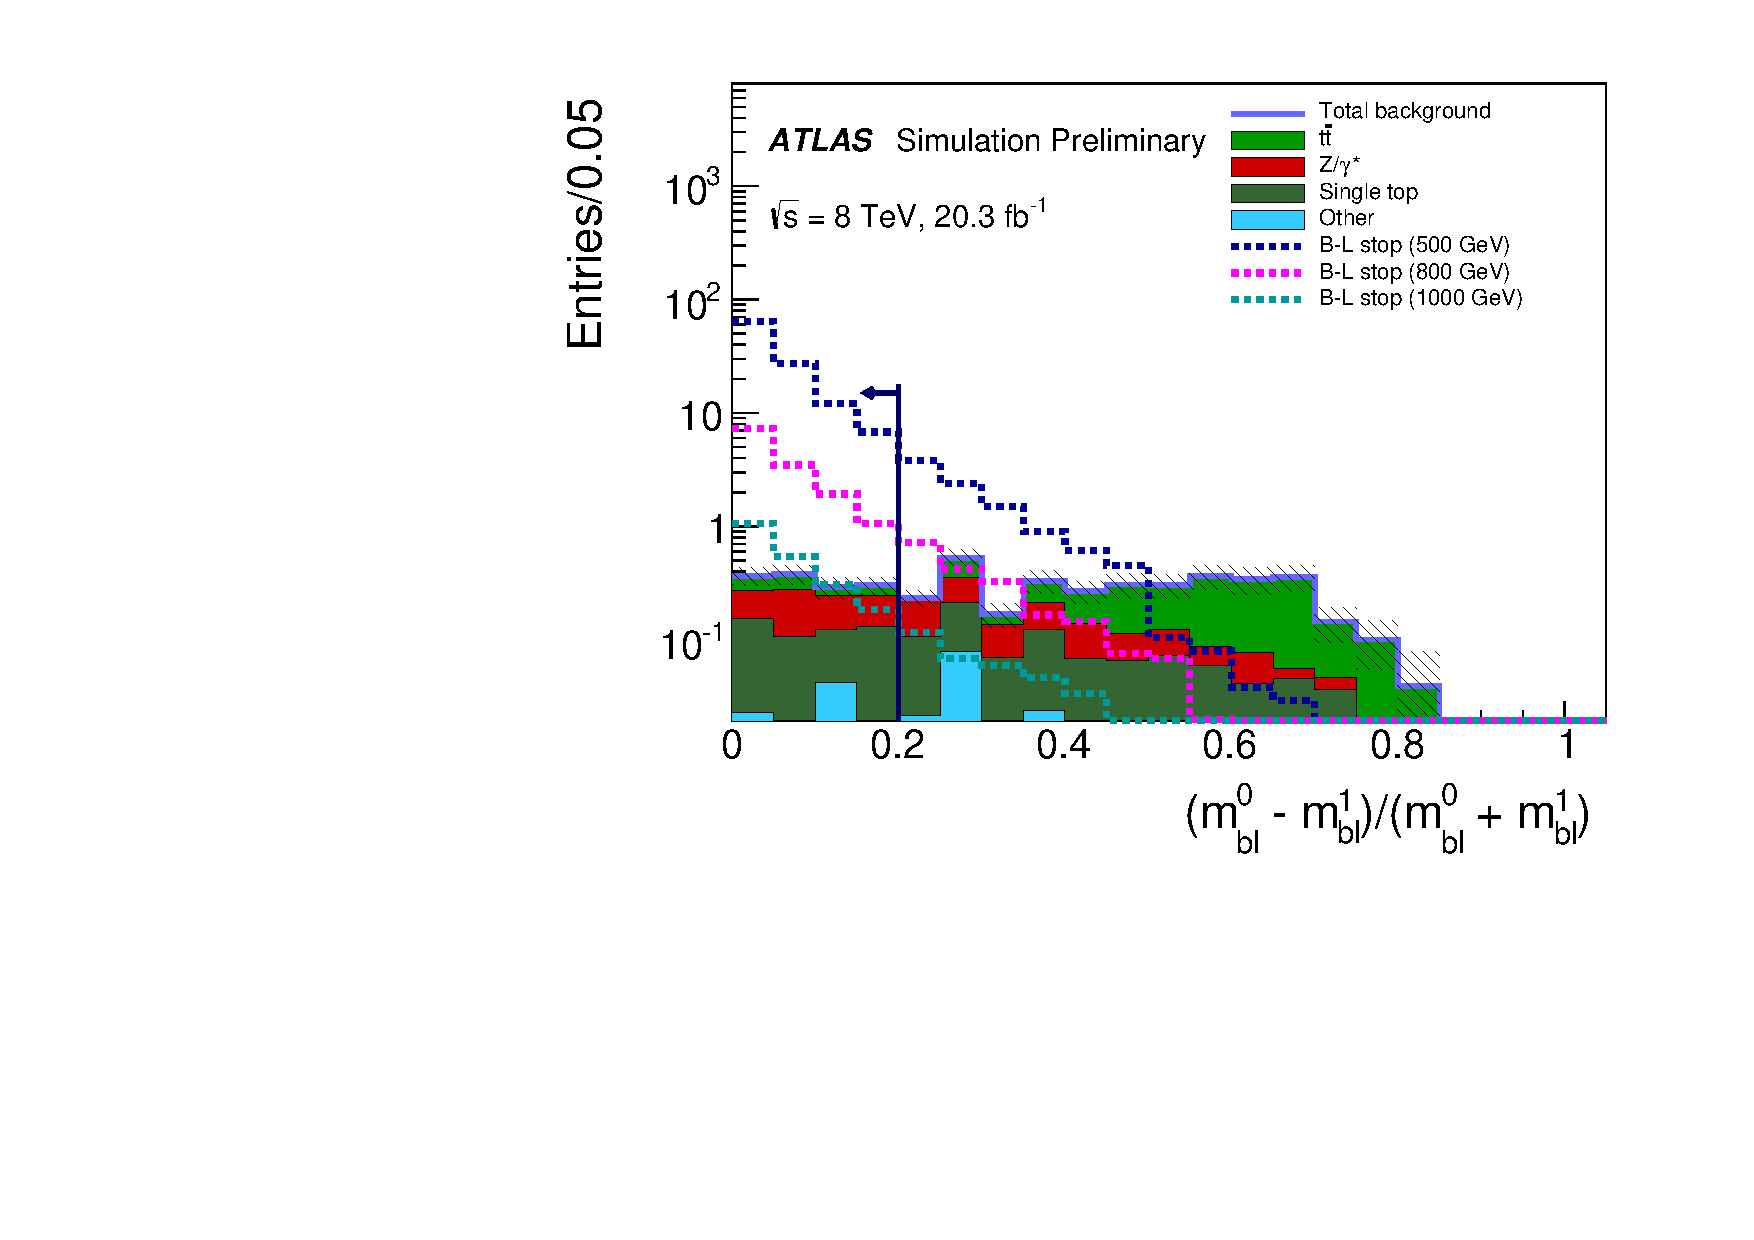
\includegraphics[width=0.48\textwidth, clip=true, trim=0 0 1cm 0]
      {figs/blstop/mbl_asym_sr_400_minus_mbl_asym.pdf}
  }
  \subbottom[$\MBL^0$]{
    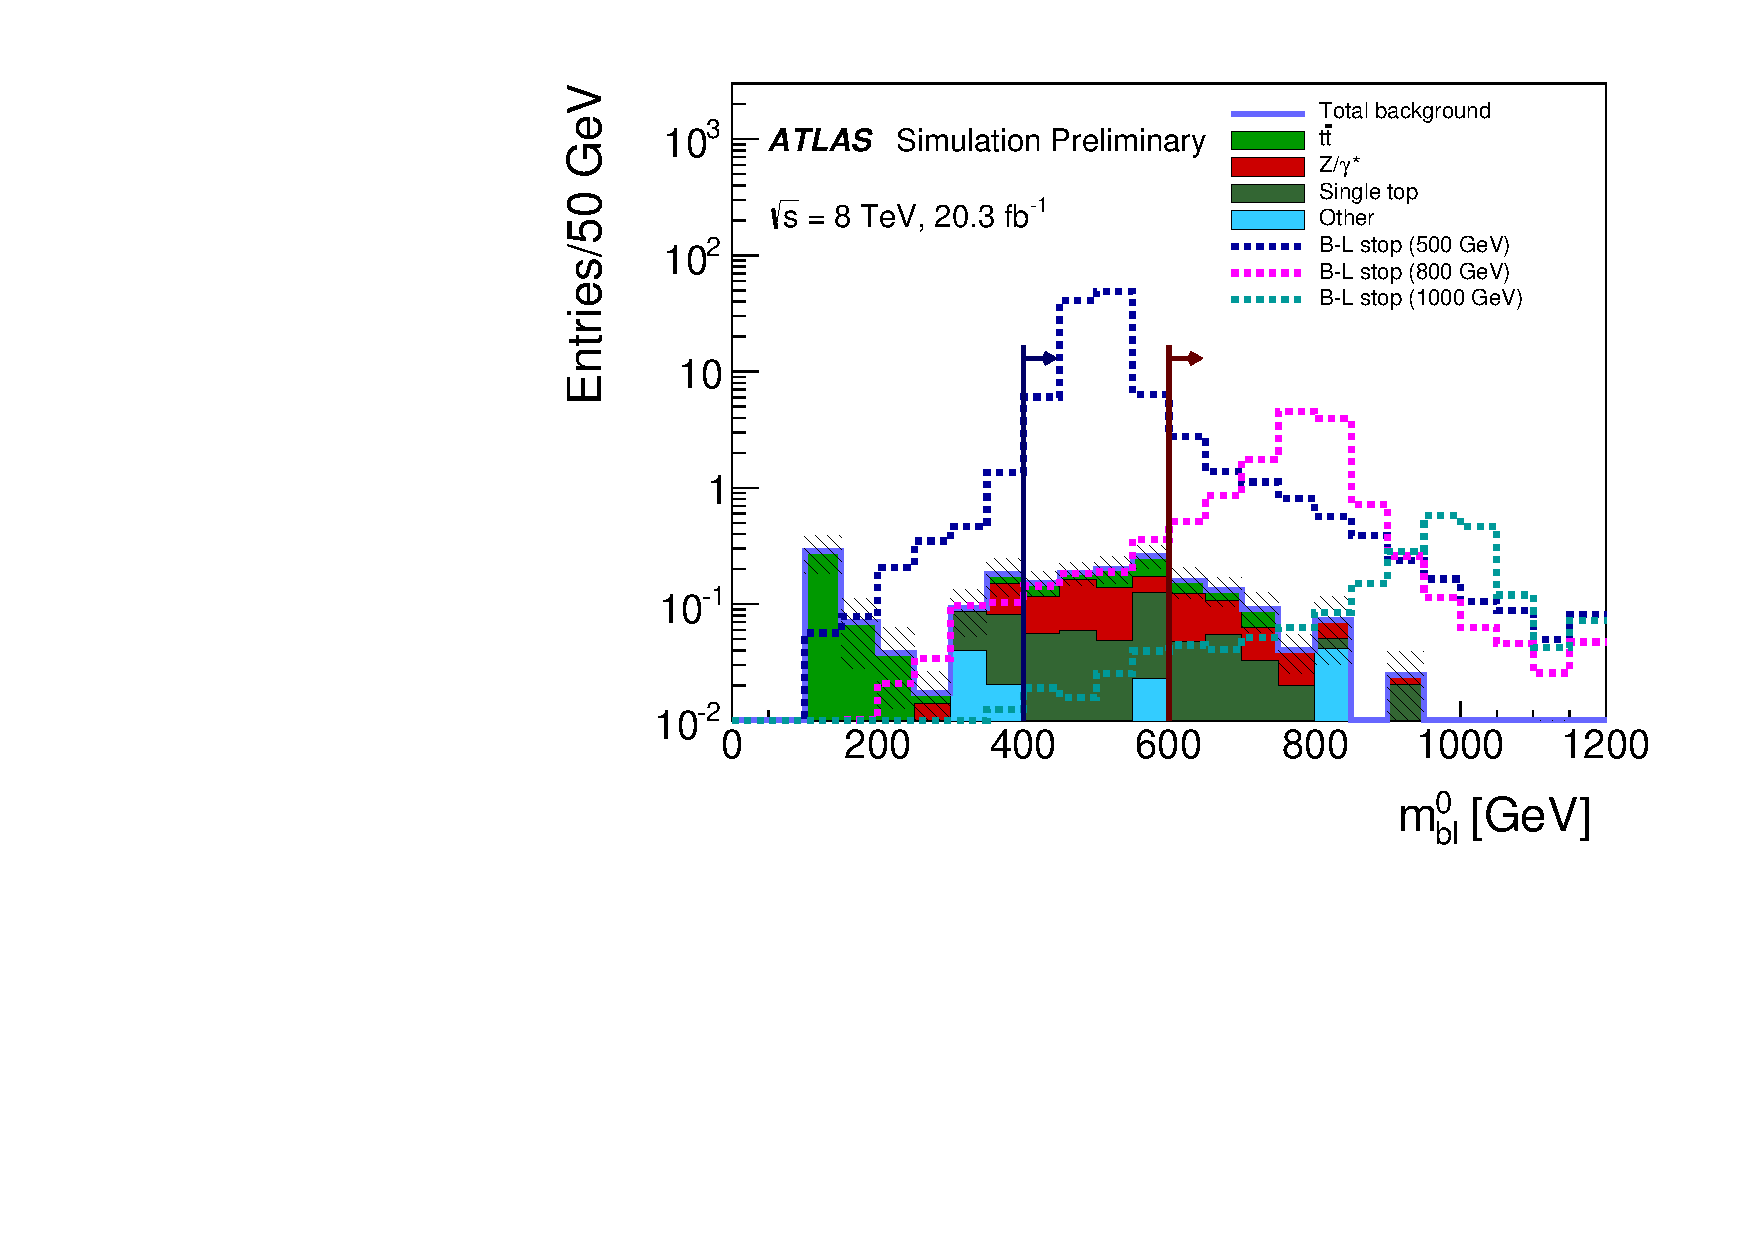
\includegraphics[width=0.48\textwidth, clip=true, trim=0 0 1cm 0]
      {figs/blstop/mbl_0_sr_minus_mbl.pdf}
  }
  \caption{Distributions of the variables which are used to define the SRs.
    These plots show the MC simulated background samples and three signal
    models, and are made after applying all the SR selection criteria except for
    that on the variable shown.
    The top two plots show the \HT\ and \MBLASYM\ variables, and the bottom
    plot shows the $\MBL^0$ distribution.
    The arrows show the SR requirement on the variable being shown.
    In each plot, the last bin includes the overflow for values beyond the
    maximum shown.
    The hashed error bands show only the statistical uncertainty in the
    background MC simulation samples.
    The signal models have an assumed
    $Br(\tilde{t}\rightarrow be) = Br(\tilde{t}\rightarrow b\mu) = 0.5$.
  }
  \label{fig:n_minus_one_sr}
  %%
\end{figure}

\begin{table}[ht]
  \caption{The number of expected signal events pasing each of the signal
    region selection criteria.
    This is shown for stop masses of 500~\GeV, 800~\GeV, and 1000~\GeV.
    The estimated yields are taken from MC simulation, and are normalized
    to 20.3~\ifb, and the uncertainty given is the MC statistical uncertainty.
    The signal models have an assumed branching fraction of
    $Br(\tilde{t}\rightarrow be) = Br(\tilde{t}\rightarrow b\mu) = 0.5$.
  }
  \label{tab:sr_cutflow}
  %
  \centering{
    \begin{tabular}{l|ccc}
      \toprule
      Selection                        & $m_{\tilde{t}} = 500 \GeV$ & $m_{\tilde{t}} = 800 \GeV$ & $m_{\tilde{t}} = 1000 \GeV$ \\
      \midrule
      $\sigma \cdot L$                 & $1750 \pm 260$             & $59 \pm 12$                & $8.9 \pm 2.5$ \\
      \midrule
      $bb\ell\ell$                     & $624 \pm 4$                & $19.65 \pm 0.18$           & $2.68 \pm 0.05$   \\
      $Z$ veto                         & $619 \pm 4$                & $19.62 \pm 0.18$           & $2.68 \pm 0.05$   \\
      $H_{T} \ge 1100 \GeV$            & $122.9 \pm 1.8$            & $16.01 \pm 0.17$           & $2.50 \pm 0.04$   \\
      $m_{b\ell}$ asymmetry $\leq 0.2$ & $112.8 \pm 1.7$            & $14.00 \pm 0.15$           & $2.11 \pm 0.04$   \\
      \midrule
      $m_{b\ell} \geq 400 \GeV$        & $110.3 \pm 1.7$            & $13.74 \pm 0.15$           & $2.09 \pm 0.04$   \\
      $m_{b\ell} \geq 600 \GeV$        & $7.7 \pm 0.4$              & $12.86 \pm 0.15$           & $1.99 \pm 0.04$   \\
      \bottomrule
    \end{tabular}
  }
\end{table}

%% -----------------------------------------------------------------------------
\FloatBarrier
\section{Background estimate}
\label{sec:bkg}

The final state targeted by this analysis is two $b$-tagged jets and two light
leptons.
The three largest sources of SM background which contribute to this final state
are \TTBAR, \ZGAMMAJETS, and single top production.
Other sources, such as di-boson and Higgs boson production, contribute as
background events as well, however in much smaller amounts.
The full list of MC simulation samples used to estimate the background
contribution from SM processes is given in Section~\ref{sec:mc_samples}.
The background estimates for the \TTBAR\ and the \ZGAMMAJETS\ backgrounds use
MC simulation normalized in dedicated data control regions (CRs).
Several validation regions (VRs) are defined to validate the extrapolation of
the fitted background estimate in the CRs to regions with different kinematics.
The remaining backgrounds are estimated using MC simulation only, and the
normalization is scaled based on the cross section of the production process and
the integrated luminosity collected in data.
The CRs and VRs are described in more detail in
Sections~\ref{sec:cr}~and~\ref{sec:vr} respectively.
The full selection criteria for the analysis regions, including the SRs, CRs,
and VRs, is outlined in Table~\ref{tab:regions} and
Figure~\ref{fig:region_coverage}.

%% - - - - - - - - - - - - - - - - - - - - - - - - - - - - - - - - - - - - - - -
\begin{table}[ht]
  \caption{Summary of signal, control, and validation regions used for this
    analysis.
    The control and validation regions are explained in Section~\ref{sec:bkg}.
    All regions require two $b$-tagged jets and two oppositely charged leptons.
    An event is in the $Z$ window if it contains two same-flavored leptons with
    an invariant mass within 10~\GeV\ of the mass of the $Z$ boson.
  }
  \label{tab:regions}
  %
  \centering{
    \begin{tabular}{l|ccccc}
      \toprule
      Region &
      $\MBL^0$ [\GeV] &
      \HT [\GeV] &
      \METSIG\ [$\GeV^{1/2}$] &
      \MBLASYM &
      $Z$ window \\
      \midrule
      SR~400   & $\geq 400$  & $\geq 1100$ & --       & $\leq 0.2$ & Veto   \\[1ex]
      SR~600   & $\geq 600$  & $\geq 1100$ & --       & $\leq 0.2$ & Veto   \\
      \midrule
      Top CR   & $\geq 200$  & $\leq 500$  & $\geq 4$ & $\leq 0.2$ & Veto   \\[1ex]
      $Z$ CR   & $\geq 200$  & $\leq 500$  & $\leq 4$ & $\leq 0.2$ & Select \\
      \midrule
      Top VR 1 & $\geq 200$  & $\leq 500$  & $< 4$    & $\leq 0.2$ & Veto   \\[1ex]
      Top VR 2 & $\geq 200$  & $\leq 500$  & -        & $>    0.2$ & Veto   \\[1ex]
      Top VR 3 & $\geq 200$  & $>   500$   & $> 4$    & $>    0.2$ & Veto   \\[1ex]
      $Z$ VR   & $\geq 200$  & $>   500$   & --       & $\leq 0.2$ & Select \\
      \bottomrule
    \end{tabular}
  }
\end{table}

%% - - - - - - - - - - - - - - - - - - - - - - - - - - - - - - - - - - - - - - -
\begin{figure}[ht]
  \centering
  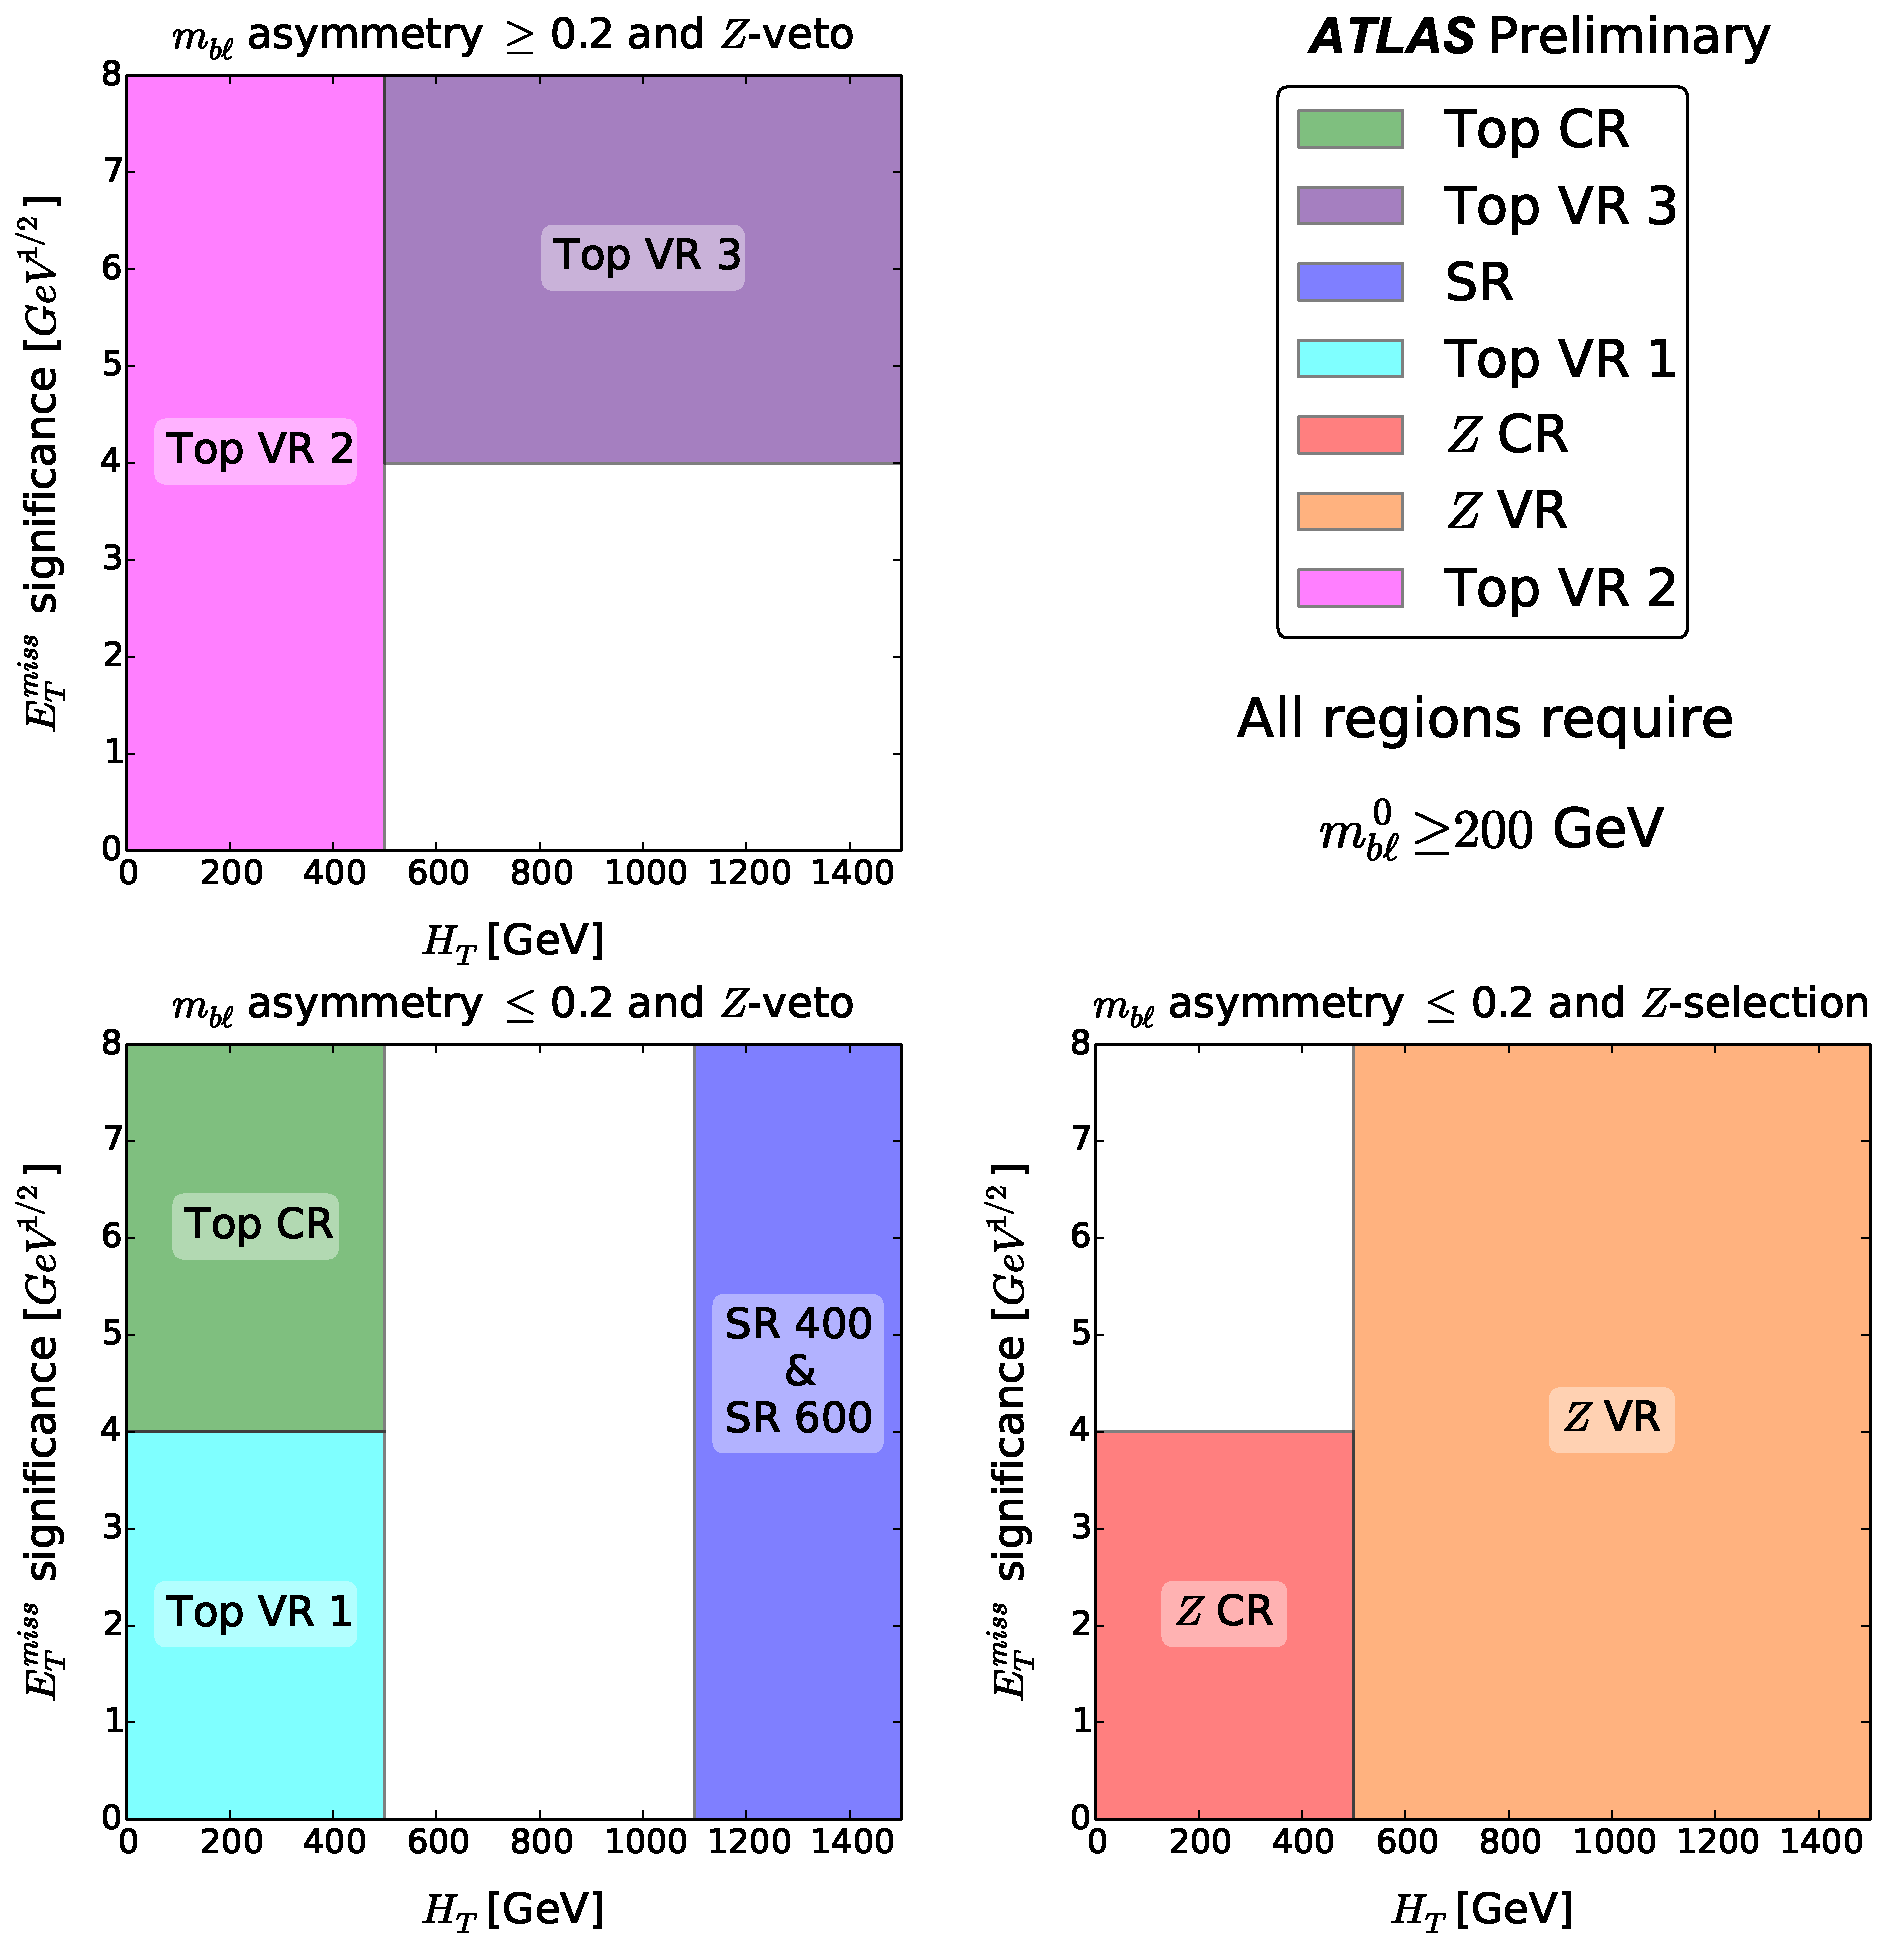
\includegraphics[width=\textwidth]{figs/blstop/regions__met_sig__ht_plane.pdf}
  \caption{Position of the regions in the \METSIG\ versus \HT\ space.
    The two left plots show the \METSIG-\HT~plane after vetoing events within
    the $Z$ window, with the top plot requiring $\MBLASYM \geq 0.2$ and the
    bottom requiring $\MBLASYM \leq 0.2$.
    The right plot shows the plane when requiring events be within the $Z$
    window.
    The two SRs apply a different requirement on the
    invariant mass of the higher-mass $b\ell$ pair. SR~400 requires
    $\MBL^{0} \geq 400 \GeV$, and SR~600 requires $\MBL^{0} \geq 600 \GeV$.
  }
  \label{fig:region_coverage}
\end{figure}

The \TTBAR\ and \ZGAMMAJETS\ normalization factors are determined using a
simultaneous fit to the data in the CRs, allowing the normalization of each
background to float independent of one another to obtain the best agreement
between the prediction and observation in the CRs.
The background fit procedure and results are described in
Section~\ref{sec:bkg_fit}.
In addition to the statistical uncertainty, several sources of systematic
uncertainty, described in Section~\ref{sec:systematics}, are considered when
performing the simultaneous fit.


%% -----------------------------------------------------------------------------
\FloatBarrier
\subsection{Monte Carlo simulation samples}
\label{sec:mc_samples}

MC simulation samples are used to estimate the selection efficiency
and kinematic distributions for SM processes.
The \TTBAR, \ZGAMMAJETS, and single top
production processes are shown separately, while all the other SM background
processes are grouped into an ``other'' category.
The \TTBAR\ background is modeled using the next-to-leading order (NLO)
generator \POWHEG\ 
revision~2129~\cite{Nason:2004rx, Frixione:2007vw, Alioli:2010xd,
Frixione:2007nw} with NLO PDF set CTEQ 6L1~\cite{Nadolsky:2008zw}, and 
showered with \PYTHIA\ version 6.426.
When using the baseline \POWHEG+\PYTHIA\ \TTBAR\ production sample,
events are reweighted in bins of the transverse mass (\pt) of the
$t\bar{t}$ system to match the top quark pair differential cross section
observed in ATLAS data~\cite{Aad:2012hg,Aad:2014zka}.
The $Wt$-channel and $s$-channel of the single top background are modeled using
\POWHEG\ revision~1556~\cite{Alioli:2009je}
with \PYTHIA\ version 6.426, while the $t$-channel is modeled using
\acermc\ version 3.8~\cite{Kersevan:2004yg} with \PYTHIA\ version 6.426,
both with PDF set CTEQ 6L1~\cite{Nadolsky:2008zw}.
The \ZGAMMAJETS\ production process is modeled using
\SHERPA\ version~1.4.1~\cite{Gleisberg:2008ta} with NLO PDF set CT10.
Charm and bottom quarks are treated as massive.

Various filters are applied to the \ZGAMMAJETS\ samples to achieve
reasonable coverage of final states and kinematics in the finite MC simulation
samples.
A dedicated set of samples are generated for each of the di-lepton flavor
combinations from the $Z$~boson ($ee$, $\mu\mu$, and $\tau\tau$).
Filters are also applied based on the quark content of the simulated event.
Samples are generated with a filter requiring at least one $b$-quark in the
event.
These samples have the largest contribution to the final background estimate.
Samples are also produced which require at least one $c$-quark, but veto events
including a $b$-quark.
The last set of samples is generated which vetoes events with either $b$-quark
or $c$-quark content.
The samples are further sliced by the \pt\ of the $Z$~boson.
Dedicated samples with generator filters are produced in slices above 40~\GeV,
and an inclusive sample is used to cover the kinematic space with
$\pt^{Z} \leq 40~\GeV$.
To avoid overlap between the inclusive sample and the higher $\pt^{Z}$ slices,
an additional requirement of $\pt^{Z,\mathrm{truth}} \leq 40 \GeV$ is applied
for the inclusive \ZGAMMAJETS\ samples simulated used \sherpa.
As \sherpa\ does not include the intermediate $Z$~boson in the truth record,
the $\pt^{Z,\mathrm{truth}}$ quantity is obtained by searching through all the
truth leptons in the event, picking the two leptons with a parent ID
consistent with a $Z$~boson, and calculating the \pt\ of the (truth level) 
di-lepton pair.

Similar filters to the \ZGAMMAJETS\ MC samples are applied to the Drell Yan (DY)
samples.
The DY samples apply the same filters on the lepton flavor combinations
and the quark content.
Rather than slicing based on the \pt\ of the $Z$~boson, the DY samples are
sliced based on the mass of the off-shell $Z/\gamma^{*}$ in the event.
Two sets of samples are produced with requirements of
$8 \leq m_{Z/\gamma^{*}}^\mathrm{truth} \leq 15 \GeV$ and 
$15 \leq m_{Z/\gamma^{*}}^\mathrm{truth} \leq 40 \GeV$ respectively, where
$m_{Z/\gamma^{*}}$ is obtained by searching through the truth record for the
decay products of the $Z/\gamma^{*}$, and computing the (truth level) invariant
mass of the di-lepton pair.

The full list of background samples used, as well as the event generator used,
SM production cross section, and the effective luminosity generated is given in 
Tables~\ref{tab:background_grouping}
and \ref{tab:background_grouping_other}.\footnote{The effective luminosity is
given by $\nicefrac{N_\mathrm{gen}\sigma}{\epsilon_\mathrm{filter}}$, where
$N_\mathrm{gen}$ is the number of MC events which were generated, $\sigma$ is
the production cross section, and $\epsilon_\mathrm{filter}$ is the efficiency
of any filter which was applied to the MC sample.}
Unless \pythia8 is specified, \pythia\ version 6 is used for samples labeled
with \pythia.

The MC simulation is generated with an assumption on the distribution of
the number of simulated interactions per crossing that differs from that
recorded in the data.
A weight is applied to the MC samples based on this difference.

Additionally, several of the MC generators provide event weights, which can
be positive or negative.
These weights account for the diagram subtraction that enters the NLL or NLO
calculations, and are commonly referred to as the ``MC event weight.''
When the generator provides MC event weights, they are applied to each event in
the MC background sample; otherwise, they are not used.

\begin{table}[ht]
  \caption{Partial summary of background samples and their cross sections used
    in this analysis except for the ``other'' category (summarized
    in Table~\ref{tab:background_grouping_other})
    The \ZGAMMAJETS\ samples are sliced by the \pt\ of the $Z$~boson.
    For the inclusive sample, only events with $\pt^{Z} \le 40 \GeV$ were used.
    For each \pt\ slice, nine samples were generated, with different lepton
    flavor channels and filters applied on the jet flavor.
    The three samples are generated with the same cross section,
    but different filter efficiencies, leading to different effective
    luminosities.
    The three columns under the effective luminosity represent the three
    samples.
    The left column shows the effective luminosity for the sample generated
    with a $b$-filter.
    The middle column represents the sample with a $c$-filter and $b$-veto.
    The right column shows the effective luminosity of the sample generated
    with a veto on both $b$- and $c$-quarks.
  }
  \label{tab:background_grouping}
  \centering{
    \begin{tabular}{c|cccccc}
      \toprule
      Grouping                      & Process                                          & Cross-section [pb]                    & \multicolumn{3}{c}{Luminosity [$\mathrm{fb}^{-1}$]} & Generator \\
      \midrule
      \TTBAR                        & \TTBAR                                           & 253                                   & \multicolumn{3}{c}{727.4}                                                                                 & \powheg+\pythia \\
      \midrule
      \multirow{3}{*}{Single top}   & $t$-channel                                      & 25.8                                  & \multicolumn{3}{c}{320}                                                                                   & \acermc+\pythia \\
                                    & $s$-channel                                      & 1.64                                  & \multicolumn{3}{c}{330}                                                                                   & \powheg+\pythia \\
                                    & $Wt$-channel                                     & 2.15                                  & \multicolumn{3}{c}{4200}                                                                                  & \powheg+\pythia \\
      \midrule
      \multirow{15}{*}{\ZGAMMAJETS} & $Z \rightarrow \ell\ell (ee, \mu\mu, \tau\tau)$  & 1110                                  & 110                                                 & 9                           & 6                     & \sherpa  \\ [1ex]
                                    & $Z \rightarrow \ell\ell (ee, \mu\mu, \tau\tau)$  & \multirow{2}{*}{70.5}                 & \multirow{2}{*}{110}                                & \multirow{2}{*}{22}         & \multirow{2}{*}{30}   & \multirow{2}{*}{\sherpa} \\
                                    & $p_{T}^{Z} \in [40 ,70] \GeV$                    & & & & &  \\ [1ex]
                                    & $Z \rightarrow \ell\ell (ee, \mu\mu, \tau\tau)$  & \multirow{2}{*}{29.5}                 & \multirow{2}{*}{510}                                & \multirow{2}{*}{90}         & \multirow{2}{*}{110}  & \multirow{2}{*}{\sherpa} \\
                                    & $p_{T}^{Z} \in [70 ,140] \GeV$                   & & & & &  \\ [1ex]
                                    & $Z \rightarrow \ell\ell (ee, \mu\mu, \tau\tau)$  & \multirow{2}{*}{3.99}                 & \multirow{2}{*}{470}                                & \multirow{2}{*}{240}        & \multirow{2}{*}{250}  & \multirow{2}{*}{\sherpa} \\
                                    & $p_{T}^{Z} \in [140,280] \GeV$                   & & & & &  \\ [1ex]
                                    & $Z \rightarrow \ell\ell (ee, \mu\mu, \tau\tau)$  & \multirow{2}{*}{0.24}                 & \multirow{2}{*}{680}                                & \multirow{2}{*}{480}        & \multirow{2}{*}{360}  & \multirow{2}{*}{\sherpa} \\
                                    & $p_{T}^{Z} \in [280,500] \GeV$                   & & & & &  \\ [1ex]
                                    & $Z \rightarrow \ell\ell (ee, \mu\mu, \tau\tau)$  & \multirow{2}{*}{$1.3 \times 10^{-2}$} & \multirow{2}{*}{5700}                               & \multirow{2}{*}{1700}       & \multirow{2}{*}{7000} & \multirow{2}{*}{\sherpa} \\
                                    & $p_{T}^{Z} \ge 500 \GeV$                         & & & & &  \\ [1ex]
                                    & DY $\rightarrow \ell\ell (ee, \mu\mu, \tau\tau)$ & \multirow{2}{*}{92.1}                 & \multicolumn{3}{c}{\multirow{2}{*}{50}}                                                                   & \multirow{2}{*}{\sherpa} \\
                                    & $m_{Z/\gamma^{*}} \in [8 ,15] \GeV$              & & & & &  \\ [1ex]
                                    & DY $\rightarrow \ell\ell (ee, \mu\mu, \tau\tau)$ & \multirow{2}{*}{279}                  & \multicolumn{3}{c}{\multirow{2}{*}{50}}                                                                   & \multirow{2}{*}{\sherpa} \\
                                    & $m_{Z/\gamma^{*}} \in [15,40] \GeV$              & & & & &  \\
      \bottomrule
    \end{tabular}
  }
\end{table}

%% \begin{table}[ht]
%%   \caption{Partial summary of background samples and their cross sections used
%%     in this analysis except for the \ZGAMMAJETS\ background (summarized in
%%     Table~\ref{tab:background_grouping_z}) and the ``other'' category (summarized
%%     in Table~\ref{tab:background_grouping_other})
%%   }
%%   \label{tab:background_grouping}
%%   \centering{
%%     \begin{tabular}{c|cccc}
%%       \toprule
%%       Grouping                    & Process      & Cross-section [pb] & Luminosity [$\mathrm{fb}^{-1}$] & Generator \\
%%       \midrule
%%       \TTBAR                      & \TTBAR       & 253                & 727.4                           & \powheg+\pythia \\
%%       \midrule
%%       \multirow{3}{*}{Single top} & $t$-channel  & 25.8               & 320                             & \acermc+\pythia \\
%%                                   & $s$-channel  & 1.64               & 330                             & \powheg+\pythia \\
%%                                   & $Wt$-channel & 2.15               & 4200                            & \powheg+\pythia \\
%%       \bottomrule
%%     \end{tabular}
%%   }
%% \end{table}


%% \begin{table}[ht]
%%   \caption{Summary of the \ZGAMMAJETS\ background samples and their cross
%%     sections used in this analysis.
%%     The \ZGAMMAJETS\ samples are sliced by the \pt\ of the $Z$~boson.
%%     For the inclusive sample, only events with $\pt^{Z} \le 40 \GeV$ were used.
%%     For each \pt\ slice, nine samples were generated, with different lepton
%%     flavor channels and filters applied on the jet flavor.
%%     The three samples are generated with approximately the same cross section,
%%     but the different filter efficiencies lead to different effective
%%     luminosities.
%%     The three columns under the effective luminosity represent the three
%%     samples.
%%     The left column shows the effective luminosity for the sample generated
%%     with a $b$-filter.
%%     The middle column represents the sample with a $c$-filter and $b$-veto.
%%     The right column shows the effective luminosity of the sample generated
%%     with a veto on both $b$- and $c$-quarks.
%%   }
%%   \label{tab:background_grouping_z}
%%   \centering{
%%     %% \resizebox{0.90\linewidth}{!}{
%%     %%   \begin{tabular}{c|cccccc}
%%     %%     \toprule
%%     %%     Grouping                       & Process                                                         & Cross-section [pb]   & \multicolumn{3}{c}{Luminosity [$\mathrm{fb}^{-1}$]} & Generator \\
%%     %%     \midrule
%%     %%     \multirow{24}{*}{\ZGAMMAJETS}  & $Z \rightarrow ee$                                              & 1110                 & 110                                                 & 9            & 6    & \sherpa \\
%%     %%                                    & $Z \rightarrow \mu\mu$                                          & 1110                 & 110                                                 & 9            & 6    & \sherpa \\
%%     %%                                    & $Z \rightarrow \tau\tau$                                        & 1110                 & 110                                                 & 9            & 6    & \sherpa \\
%%     %%                                    & $Z \rightarrow ee$        ($p_{T}^{Z} \in [40 ,70] \GeV$)       & 70.5                 & 110                                                 & 22           & 30   & \sherpa \\
%%     %%                                    & $Z \rightarrow \mu\mu$    ($p_{T}^{Z} \in [40 ,70] \GeV$)       & 70.5                 & 110                                                 & 22           & 30   & \sherpa \\
%%     %%                                    & $Z \rightarrow \tau\tau$  ($p_{T}^{Z} \in [40 ,70] \GeV$)       & 70.5                 & 110                                                 & 22           & 30   & \sherpa \\
%%     %%                                    & $Z \rightarrow ee$        ($p_{T}^{Z} \in [70 ,140] \GeV$)      & 29.5                 & 510                                                 & 90           & 110  & \sherpa \\
%%     %%                                    & $Z \rightarrow \mu\mu$    ($p_{T}^{Z} \in [70 ,140] \GeV$)      & 29.5                 & 510                                                 & 90           & 110  & \sherpa \\
%%     %%                                    & $Z \rightarrow \tau\tau$  ($p_{T}^{Z} \in [70 ,140] \GeV$)      & 29.5                 & 510                                                 & 90           & 110  & \sherpa \\
%%     %%                                    & $Z \rightarrow ee$        ($p_{T}^{Z} \in [140,280] \GeV$)      & 3.99                 & 470                                                 & 240          & 250  & \sherpa \\
%%     %%                                    & $Z \rightarrow \mu\mu$    ($p_{T}^{Z} \in [140,280] \GeV$)      & 3.99                 & 470                                                 & 240          & 250  & \sherpa \\
%%     %%                                    & $Z \rightarrow \tau\tau$  ($p_{T}^{Z} \in [140,280] \GeV$)      & 3.99                 & 470                                                 & 240          & 250  & \sherpa \\
%%     %%                                    & $Z \rightarrow ee$        ($p_{T}^{Z} \in [280,500] \GeV$)      & 0.24                 & 680                                                 & 480          & 360  & \sherpa \\
%%     %%                                    & $Z \rightarrow \mu\mu$    ($p_{T}^{Z} \in [280,500] \GeV$)      & 0.24                 & 680                                                 & 480          & 360  & \sherpa \\
%%     %%                                    & $Z \rightarrow \tau\tau$  ($p_{T}^{Z} \in [280,500] \GeV$)      & 0.24                 & 680                                                 & 480          & 360  & \sherpa \\
%%     %%                                    & $Z \rightarrow ee$        ($p_{T}^{Z} \ge 500 \GeV$)            & $1.3 \times 10^{-2}$ & 5700                                                & 1700         & 7000 & \sherpa \\
%%     %%                                    & $Z \rightarrow \mu\mu$    ($p_{T}^{Z} \ge 500 \GeV$)            & $1.3 \times 10^{-2}$ & 5700                                                & 1700         & 7000 & \sherpa \\
%%     %%                                    & $Z \rightarrow \tau\tau$  ($p_{T}^{Z} \ge 500 \GeV$)            & $1.3 \times 10^{-2}$ & 5700                                                & 1700         & 7000 & \sherpa \\
%%     %%                                    & DY $\rightarrow ee$       ($m_{Z/\gamma^{*}} \in [8 ,15] \GeV$) & 92.1                 & \multicolumn{3}{c}{50}                              & \sherpa \\
%%     %%                                    & DY $\rightarrow \mu\mu$   ($m_{Z/\gamma^{*}} \in [8 ,15] \GeV$) & 92.1                 & \multicolumn{3}{c}{50}                              & \sherpa \\
%%     %%                                    & DY $\rightarrow \tau\tau$ ($m_{Z/\gamma^{*}} \in [8 ,15] \GeV$) & 92.1                 & \multicolumn{3}{c}{50}                              & \sherpa \\
%%     %%                                    & DY $\rightarrow ee$       ($m_{Z/\gamma^{*}} \in [15,40] \GeV$) & 279                  & \multicolumn{3}{c}{50}                              & \sherpa \\
%%     %%                                    & DY $\rightarrow \mu\mu$   ($m_{Z/\gamma^{*}} \in [15,40] \GeV$) & 279                  & \multicolumn{3}{c}{50}                              & \sherpa \\
%%     %%                                    & DY $\rightarrow \tau\tau$ ($m_{Z/\gamma^{*}} \in [15,40] \GeV$) & 279                  & \multicolumn{3}{c}{50}                              & \sherpa \\
%%     %%     \bottomrule
%%     %%   \end{tabular}
%%     %% }
%%     % \resizebox{0.90\linewidth}{!}{
%%       \begin{tabular}{c|cccccc}
%%         \toprule
%%         Grouping                      & Process                                          & Cross-section [pb]                    & \multicolumn{3}{c}{Luminosity [$\mathrm{fb}^{-1}$]} & Generator \\
%%         \midrule
%%         \multirow{15}{*}{\ZGAMMAJETS} & $Z \rightarrow \ell\ell (ee, \mu\mu, \tau\tau)$  & 1110                                  & 110                                                 & 9                           & 6                     & \sherpa  \\ [1ex]
%%                                       & $Z \rightarrow \ell\ell (ee, \mu\mu, \tau\tau)$  & \multirow{2}{*}{70.5}                 & \multirow{2}{*}{110}                                & \multirow{2}{*}{22}         & \multirow{2}{*}{30}   & \multirow{2}{*}{\sherpa} \\
%%                                       & $p_{T}^{Z} \in [40 ,70] \GeV$                    & & & & &  \\ [1ex]
%%                                       & $Z \rightarrow \ell\ell (ee, \mu\mu, \tau\tau)$  & \multirow{2}{*}{29.5}                 & \multirow{2}{*}{510}                                & \multirow{2}{*}{90}         & \multirow{2}{*}{110}  & \multirow{2}{*}{\sherpa} \\
%%                                       & $p_{T}^{Z} \in [70 ,140] \GeV$                   & & & & &  \\ [1ex]
%%                                       & $Z \rightarrow \ell\ell (ee, \mu\mu, \tau\tau)$  & \multirow{2}{*}{3.99}                 & \multirow{2}{*}{470}                                & \multirow{2}{*}{240}        & \multirow{2}{*}{250}  & \multirow{2}{*}{\sherpa} \\
%%                                       & $p_{T}^{Z} \in [140,280] \GeV$                   & & & & &  \\ [1ex]
%%                                       & $Z \rightarrow \ell\ell (ee, \mu\mu, \tau\tau)$  & \multirow{2}{*}{0.24}                 & \multirow{2}{*}{680}                                & \multirow{2}{*}{480}        & \multirow{2}{*}{360}  & \multirow{2}{*}{\sherpa} \\
%%                                       & $p_{T}^{Z} \in [280,500] \GeV$                   & & & & &  \\ [1ex]
%%                                       & $Z \rightarrow \ell\ell (ee, \mu\mu, \tau\tau)$  & \multirow{2}{*}{$1.3 \times 10^{-2}$} & \multirow{2}{*}{5700}                               & \multirow{2}{*}{1700}       & \multirow{2}{*}{7000} & \multirow{2}{*}{\sherpa} \\
%%                                       & $p_{T}^{Z} \ge 500 \GeV$                         & & & & &  \\ [1ex]
%%                                       & DY $\rightarrow \ell\ell (ee, \mu\mu, \tau\tau)$ & \multirow{2}{*}{92.1}                 & \multicolumn{3}{c}{\multirow{2}{*}{50}}                                                                   & \multirow{2}{*}{\sherpa} \\
%%                                       & $m_{Z/\gamma^{*}} \in [8 ,15] \GeV$              & & & & &  \\ [1ex]
%%                                       & DY $\rightarrow \ell\ell (ee, \mu\mu, \tau\tau)$ & \multirow{2}{*}{279}                  & \multicolumn{3}{c}{\multirow{2}{*}{50}}                                                                   & \multirow{2}{*}{\sherpa} \\
%%                                       & $m_{Z/\gamma^{*}} \in [15,40] \GeV$              & & & & &  \\
%%         \bottomrule
%%       \end{tabular}
%%     % }
%%   }
%% \end{table}

\begin{table}[ht]
  \caption{Summary of other background samples and their cross sections used in
    this analysis.
    The $W \rightarrow \ell\nu$ and $Z \rightarrow \ell\ell$ processes each have 
    dedicated samples for each lepton flavor as indicated in the parentheses.
    The $W$ samples are generated with filters on the jet flavor.
    As in Table~\ref{tab:background_grouping}, the three columns under the
    effective luminosity represent the three samples ($b$-filter, $c$-filter
    and $b$-veto, veto on both $b$- and $c$-quarks).
  }
  \label{tab:background_grouping_other}
  \centering{
    %% \resizebox{0.90\linewidth}{!}{
    %%   \begin{tabular}{c|cccccc}
    %%     \toprule
    %%     Grouping &
    %%     Process &
    %%     Cross-section [pb] &
    %%     \multicolumn{3}{c}{Luminosity [$\mathrm{fb}^{-1}$]} &
    %%     Generator \\
    %%     \midrule
    %%     \multirow{50}{*}{Other}  & $\TTBAR\,W$                                                     & 0.10                 & \multicolumn{3}{c}{3300 }              & \madgraph+\pythia \\
    %%                              & $\TTBAR\,Wj$                                                    & $9.3 \times 10^{-2}$ & \multicolumn{3}{c}{3600 }              & \madgraph+\pythia \\
    %%                              & $\TTBAR\,Z$                                                     & $6.8 \times 10^{-2}$ & \multicolumn{3}{c}{4400 }              & \madgraph+\pythia \\
    %%                              & $\TTBAR\,Zj$                                                    & $8.7 \times 10^{-2}$ & \multicolumn{3}{c}{3400 }              & \madgraph+\pythia \\
    %%                              & $\TTBAR\,WW$                                                    & $9.2 \times 10^{-4}$ & \multicolumn{3}{c}{11000}              & \madgraph+\pythia \\
    %%                              & $WW \rightarrow \ell\ell\nu\nu$                                 & 5.30                 & \multicolumn{3}{c}{1400 }              & \sherpa           \\
    %%                              & $WW \rightarrow e\nu qq$                                        & 7.29                 & \multicolumn{3}{c}{100  }              & \sherpa           \\
    %%                              & $WW \rightarrow \mu\nu qq$                                      & 7.30                 & \multicolumn{3}{c}{100  }              & \sherpa           \\
    %%                              & $WW \rightarrow \tau\nu qq$                                     & 7.27                 & \multicolumn{3}{c}{100  }              & \sherpa           \\
    %%                              & $WZ \rightarrow \ell\ell\ell\nu$                                & 9.74                 & \multicolumn{3}{c}{260  }              & \sherpa           \\
    %%                              & $WZ \rightarrow \ell\nu\nu\nu$                                  & 1.40                 & \multicolumn{3}{c}{270  }              & \sherpa           \\
    %%                              & $WZ \rightarrow e\nu qq$                                        & 1.90                 & \multicolumn{3}{c}{110  }              & \sherpa           \\
    %%                              & $WZ \rightarrow \mu\nu qq$                                      & 1.91                 & \multicolumn{3}{c}{100  }              & \sherpa           \\
    %%                              & $WZ \rightarrow \tau\nu qq$                                     & 1.92                 & \multicolumn{3}{c}{100  }              & \sherpa           \\
    %%                              & $WZ \rightarrow ee qq$                                          & 1.46                 & \multicolumn{3}{c}{110  }              & \sherpa           \\
    %%                              & $WZ \rightarrow \mu\mu qq$                                      & 1.46                 & \multicolumn{3}{c}{110  }              & \sherpa           \\
    %%                              & $WZ \rightarrow \tau\tau qq$                                    & 1.45                 & \multicolumn{3}{c}{120  }              & \sherpa           \\
    %%                              & $WZ \rightarrow \nu\nu qq$                                      & 2.70                 & \multicolumn{3}{c}{64   }              & \sherpa           \\
    %%                              & $ZZ \rightarrow \ell\ell\nu\nu$                                 & 0.49                 & \multicolumn{3}{c}{1700 }              & \sherpa           \\
    %%                              & $ZZ \rightarrow ee qq$                                          & 0.25                 & \multicolumn{3}{c}{120  }              & \sherpa           \\
    %%                              & $ZZ \rightarrow \mu\mu qq$                                      & 0.25                 & \multicolumn{3}{c}{120  }              & \sherpa           \\
    %%                              & $ZZ \rightarrow \tau\tau qq$                                    & 0.24                 & \multicolumn{3}{c}{120  }              & \sherpa           \\
    %%                              & $ZZ \rightarrow \nu\nu qq$                                      & 1.74                 & \multicolumn{3}{c}{69   }              & \sherpa           \\
    %%                              & ggf $H \rightarrow WW$                                          & 0.44                 & \multicolumn{3}{c}{2000 }              & \powheg+\pythia 8 \\
    %%                              & ggf $H \rightarrow ZZ$                                          & $4.7 \times 10^{-2}$ & \multicolumn{3}{c}{2000 }              & \powheg+\pythia 8 \\
    %%                              & VBF $H \rightarrow WW$                                          & $3.6 \times 10^{-2}$ & \multicolumn{3}{c}{17000}              & \powheg+\pythia 8 \\
    %%                              & VBF $H \rightarrow ZZ$                                          & $3.8 \times 10^{-3}$ & \multicolumn{3}{c}{18000}              & \powheg+\pythia 8 \\
    %%                              & $WH \rightarrow W\ell\nu\ell\nu$                                & 0.15                 & \multicolumn{3}{c}{1000 }              & \pythia 8         \\
    %%                              & $WH \rightarrow W\ell\ell\nu\nu$                                & $1.7 \times 10^{-3}$ & \multicolumn{3}{c}{27000}              & \pythia 8         \\
    %%                              & $ZH \rightarrow Z\ell\nu\ell\nu$                                & $8.9 \times 10^{-3}$ & \multicolumn{3}{c}{2000 }              & \pythia 8         \\
    %%                              & $ZH \rightarrow Z\ell\ell\nu\nu$                                & $1.0 \times 10^{-2}$ & \multicolumn{3}{c}{48000}              & \pythia 8         \\
    %%                              & $\TTBAR H \rightarrow \TTBAR WW$                                & $2.8 \times 10^{-2}$ & \multicolumn{3}{c}{7000 }              & \pythia 8         \\
    %%                              & $W \rightarrow e\nu$                                            & 11000                & 100                       & 17   & 4   & \sherpa           \\
    %%                              & $W \rightarrow \mu\nu$                                          & 11000                & 100                       & 17   & 4   & \sherpa           \\
    %%                              & $W \rightarrow \tau\nu$                                         & 11000                & 100                       & 17   & 4   & \sherpa           \\
    %%                              & $W \rightarrow e\nu$    ($p_\mathrm{T}^{W} \in [40,70] \GeV$)   & 653                  & 44                        & 7    & 30  & \sherpa           \\
    %%                              & $W \rightarrow \mu\nu$  ($p_\mathrm{T}^{W} \in [40,70] \GeV$)   & 653                  & 44                        & 7    & 30  & \sherpa           \\
    %%                              & $W \rightarrow \tau\nu$ ($p_\mathrm{T}^{W} \in [40,70] \GeV$)   & 653                  & 44                        & 7    & 30  & \sherpa           \\
    %%                              & $W \rightarrow e\nu$    ($p_\mathrm{T}^{W} \in [70,140] \GeV$)  & 251                  & 160                       & 54   & 24  & \sherpa           \\
    %%                              & $W \rightarrow \mu\nu$  ($p_\mathrm{T}^{W} \in [70,140] \GeV$)  & 251                  & 160                       & 54   & 24  & \sherpa           \\
    %%                              & $W \rightarrow \tau\nu$ ($p_\mathrm{T}^{W} \in [70,140] \GeV$)  & 251                  & 160                       & 54   & 24  & \sherpa           \\
    %%                              & $W \rightarrow e\nu$    ($p_\mathrm{T}^{W} \in [140,280] \GeV$) & 31.2                 & 460                       & 260  & 80  & \sherpa           \\
    %%                              & $W \rightarrow \mu\nu$  ($p_\mathrm{T}^{W} \in [140,280] \GeV$) & 31.2                 & 460                       & 260  & 80  & \sherpa           \\
    %%                              & $W \rightarrow \tau\nu$ ($p_\mathrm{T}^{W} \in [140,280] \GeV$) & 31.2                 & 460                       & 260  & 80  & \sherpa           \\
    %%                              & $W \rightarrow e\nu$    ($p_\mathrm{T}^{W} \in [280,500] \GeV$) & 1.84                 & 590                       & 420  & 360 & \sherpa           \\
    %%                              & $W \rightarrow \mu\nu$  ($p_\mathrm{T}^{W} \in [280,500] \GeV$) & 1.84                 & 590                       & 420  & 360 & \sherpa           \\
    %%                              & $W \rightarrow \tau\nu$ ($p_\mathrm{T}^{W} \in [280,500] \GeV$) & 1.84                 & 590                       & 420  & 360 & \sherpa           \\
    %%                              & $W \rightarrow e\nu$    ($p_\mathrm{T}^{W} \ge 500 \GeV$)       & 0.10                 & 890                       & 360  & 140 & \sherpa           \\
    %%                              & $W \rightarrow \mu\nu$  ($p_\mathrm{T}^{W} \ge 500 \GeV$)       & 0.10                 & 890                       & 360  & 670 & \sherpa           \\
    %%                              & $W \rightarrow \tau\nu$ ($p_\mathrm{T}^{W} \ge 500 \GeV$)       & 0.10                 & 890                       & 360  & 670 & \sherpa           \\
    %%     \bottomrule
    %%   \end{tabular}
    %% }
      \begin{tabular}{c|cccccc}
        \toprule
        Grouping &
        Process &
        Cross-section [pb] &
        \multicolumn{3}{c}{Luminosity [$\mathrm{fb}^{-1}$]} &
        Generator \\
        \midrule
        \multirow{35}{*}{Other}    & $\TTBAR\,W$                                         & 0.10                  & \multicolumn{3}{c}{3300 } & \madgraph+\pythia \\
                                   & $\TTBAR\,Wj$                                        & $9.3 \times 10^{-2}$  & \multicolumn{3}{c}{3600 } & \madgraph+\pythia \\ [1ex]
                                   & $\TTBAR\,Z$                                         & $6.8 \times 10^{-2}$  & \multicolumn{3}{c}{4400 } & \madgraph+\pythia \\
                                   & $\TTBAR\,Zj$                                        & $8.7 \times 10^{-2}$  & \multicolumn{3}{c}{3400 } & \madgraph+\pythia \\ [1ex]
                                   & $\TTBAR\,WW$                                        & $9.2 \times 10^{-4}$  & \multicolumn{3}{c}{11000} & \madgraph+\pythia \\ [1ex]
                                   & $WW \rightarrow \ell\ell\nu\nu$                     & 5.30                  & \multicolumn{3}{c}{1400 } & \sherpa           \\
                                   & $WW \rightarrow \ell\nu qq (e,\mu,\tau)$            & 7.3                   & \multicolumn{3}{c}{100  } & \sherpa           \\ [1ex]
                                   & $WZ \rightarrow \ell\ell\ell\nu$                    & 9.74                  & \multicolumn{3}{c}{260  } & \sherpa           \\
                                   & $WZ \rightarrow \ell\nu\nu\nu$                      & 1.40                  & \multicolumn{3}{c}{270  } & \sherpa           \\
                                   & $WZ \rightarrow \ell\nu qq (e,\mu,\tau)$            & 1.9                   & \multicolumn{3}{c}{110  } & \sherpa           \\
                                   & $WZ \rightarrow \ell\ell qq (ee, \mu\mu, \tau\tau)$ & 1.46                  & \multicolumn{3}{c}{110  } & \sherpa           \\
                                   & $WZ \rightarrow \nu\nu qq$                          & 2.70                  & \multicolumn{3}{c}{64   } & \sherpa           \\ [1ex]
                                   & $ZZ \rightarrow \ell\ell\nu\nu$                     & 0.49                  & \multicolumn{3}{c}{1700 } & \sherpa           \\
                                   & $ZZ \rightarrow \ell\ell qq (ee, \mu\mu, \tau\tau)$ & 0.25                  & \multicolumn{3}{c}{120  } & \sherpa           \\
                                   & $ZZ \rightarrow \nu\nu qq$                          & 1.74                  & \multicolumn{3}{c}{69   } & \sherpa           \\ [1ex]
                                   & ggf $H \rightarrow WW$                              & 0.44                  & \multicolumn{3}{c}{2000 } & \powheg+\pythia 8 \\
                                   & ggf $H \rightarrow ZZ$                              & $4.7 \times 10^{-2}$  & \multicolumn{3}{c}{2000 } & \powheg+\pythia 8 \\
                                   & VBF $H \rightarrow WW$                              & $3.6 \times 10^{-2}$  & \multicolumn{3}{c}{17000} & \powheg+\pythia 8 \\
                                   & VBF $H \rightarrow ZZ$                              & $3.8 \times 10^{-3}$  & \multicolumn{3}{c}{18000} & \powheg+\pythia 8 \\ [1ex]
                                   & $WH \rightarrow W\ell\nu\ell\nu$                    & 0.15                  & \multicolumn{3}{c}{1000 } & \pythia 8         \\
                                   & $WH \rightarrow W\ell\ell\nu\nu$                    & $1.7 \times 10^{-3}$  & \multicolumn{3}{c}{27000} & \pythia 8         \\ [1ex]
                                   & $ZH \rightarrow Z\ell\nu\ell\nu$                    & $8.9 \times 10^{-3}$  & \multicolumn{3}{c}{2000 } & \pythia 8         \\
                                   & $ZH \rightarrow Z\ell\ell\nu\nu$                    & $1.0 \times 10^{-2}$  & \multicolumn{3}{c}{48000} & \pythia 8         \\ [1ex]
                                   & $\TTBAR H \rightarrow \TTBAR WW$                    & $2.8 \times 10^{-2}$  & \multicolumn{3}{c}{7000 } & \pythia 8         \\ [1ex]
                                   & $W \rightarrow \ell\nu (e, \mu, \tau)$              & 11000                 & 100                       & 17                   & 4                    & \sherpa \\ [1ex]
                                   & $W \rightarrow \ell\nu (e, \mu, \tau)$              & \multirow{2}{*}{653}  & \multirow{2}{*}{44}       & \multirow{2}{*}{7}   & \multirow{2}{*}{30}  & \multirow{2}{*}{\sherpa} \\
                                   & $p_\mathrm{T}^{W} \in [40,70] \GeV$                 &                       &                           &                      &                      & \\ [1ex]
                                   & $W \rightarrow \ell\nu (e, \mu, \tau)$              & \multirow{2}{*}{251}  & \multirow{2}{*}{160}      & \multirow{2}{*}{54}  & \multirow{2}{*}{24}  & \multirow{2}{*}{\sherpa} \\
                                   & $p_\mathrm{T}^{W} \in [70,140] \GeV$                &                       &                           &                      &                      & \\ [1ex]
                                   & $W \rightarrow \ell\nu (e, \mu, \tau)$              & \multirow{2}{*}{31.2} & \multirow{2}{*}{460}      & \multirow{2}{*}{260} & \multirow{2}{*}{80}  & \multirow{2}{*}{\sherpa} \\
                                   & $p_\mathrm{T}^{W} \in [140,280] \GeV$               &                       &                           &                      &                      & \\ [1ex]
                                   & $W \rightarrow \ell\nu (e, \mu, \tau)$              & \multirow{2}{*}{1.84} & \multirow{2}{*}{590}      & \multirow{2}{*}{420} & \multirow{2}{*}{360} & \multirow{2}{*}{\sherpa} \\
                                   & $p_\mathrm{T}^{W} \in [280,500] \GeV$               &                       &                           &                      &                      & \\ [1ex]
                                   & $W \rightarrow \ell\nu (e, \mu, \tau)$              & \multirow{2}{*}{0.10} & \multirow{2}{*}{890}      & \multirow{2}{*}{360} & \multirow{2}{*}{140} & \multirow{2}{*}{\sherpa} \\
                                   & $p_\mathrm{T}^{W} \ge 500 \GeV$                     &                       &                           &                      &                      &  \\
        \bottomrule
      \end{tabular}
  }
\end{table}

\FloatBarrier


%% -----------------------------------------------------------------------------
\FloatBarrier
\subsection{Control regions}
\label{sec:cr}

The normalization of the \TTBAR\ and \ZGAMMAJETS\ backgrounds are determined
using the observed data in two dedicated CRs, labeled the top control region
(Top CR) and $Z$ control region ($Z$ CR) respectively.
To reduce the uncertainty in the \TTBAR\ and \ZGAMMAJETS\ normalization factors,
the CRs are defined such that they are expected to be fairly pure in events
coming from the single background process of interest.

There must also be little signal contamination in the CRs to prevent potential
signal events from influencing the background normalization.
To reduce signal contamination, the Top and $Z$ CRs both require
$\HT \leq 500~\GeV$.
In addition to reducing the expected signal contamination, the CRs should have
kinematics as similar as possible to the SRs to make the extrapolation from the
CRs to SRs more reliable.
For this reason, a requirement of $\MBLASYM \leq 0.2$ is applied to both the
Top and $Z$ CRs to match the \MBLASYM\ requirement in the SRs.
A requirement of $\MBL^0 \geq 200 \GeV$ is applied so the background
normalization is taken from a region of $\MBL^0$ which is more similar to that
of the SRs.
Imposing a stricter requirement on $\MBL^0$ reduces the expected and observed
number of events in both CRs, and a reliable estimate of the \TTBAR\ and
\ZGAMMAJETS\ normalizations cannot be obtained due to statistical uncertainties.
No requirement is made on the $\MBL^1$.

To ensure the CRs are relatively pure in \TTBAR\ or \ZGAMMAJETS, the
missing transverse energy (\MET) is used.
Rather than select on the \MET\ alone, \METSIG\ is defined as
\begin{equation}
  \METSIG = \frac{\MET}{\sqrt{\HT}}.
\end{equation}
By scaling the \MET\ by the total amount of energy in the event, the
\METSIG\ is less susceptible to the effects of fake \MET\ from of mismeasurement
of objects in an event.
This makes the \METSIG\ more robust to the energy scale of the event.
Processes like \TTBAR\ and single top, with \MET\ in the final state from
neutrinos, tend
to have large \METSIG, while processes with \MET coming entirely from
mismeasurement, such as \ZGAMMAJETS, tend to have low values for \METSIG.
The Top CR requires $\METSIG \geq 4 \GeV^{1/2}$
and the $Z$ CR requires $\METSIG \leq 4 \GeV^{1/2}$.

Lastly, events containing like-flavor leptons, with a reconstructed invariant
mass within 10~\GeV of the $Z$~boson mass are rejected from the Top CR.
The $Z$ CR, requires events be within this $Z$ region.
The definitions of the CRs are summarized in Table~\ref{tab:regions} and
Figure~\ref{fig:region_coverage}.

The expected and observed $\MBL^{0}$ distributions in the Top CR and $Z$ CR,
shown in Figure~\ref{fig:cr_mbl_0__no_norm_factor} show reasonable agreement
between the predicted and observed data in the Top CR.
However, the normalization is underpredicted in the $Z$ CR.
This disagreement seems to be caused by a poor modeling of the
\ZGAMMAJETS\ background process when heavy flavor jets are required in the
final state.
For the final result, a maximum likelihood fit is used to determine the
normalization of the \ZGAMMAJETS\ background as described in
Section~\ref{sec:bkg_fit}; however, due to the large disagreement in the
data and MC simulation, it is useful to scale the \ZGAMMAJETS\ background based
on the observed difference in normalization for exploratory plots and tables to
obtain a more realistic estimate of the expected backgrounds in each region.
The scaling factor is calculated in the expression
\begin{equation}
  k_Z = \frac{N_\mathrm{data}^{Z~\mathrm{CR}} -
                \sum_{p \neq Z}N_{p}^{Z~\mathrm{CR}} }
             {N_{Z}^{Z~\mathrm{CR}}}
\end{equation}
where $N_\mathrm{data}^{Z~\mathrm{CR}}$ is the number of observed events in
the $Z$ CR, and $N_{p}^{Z~\mathrm{CR}}$ is the number of expected events in
$Z$ CR from process $p$ based on the MC background simulation.
This scaling factor is determined to be $k_Z = 1.39$, and will be applied to
the \ZGAMMAJETS\ background prediction in many of the plots and tables in this
section.
This normalization factor is not included in the final fit to data, and any plot
or figure which is produced using this normalization factor explicitly
states this in the description.

\begin{figure}
  \centering
  \subbottom[Top CR]{
    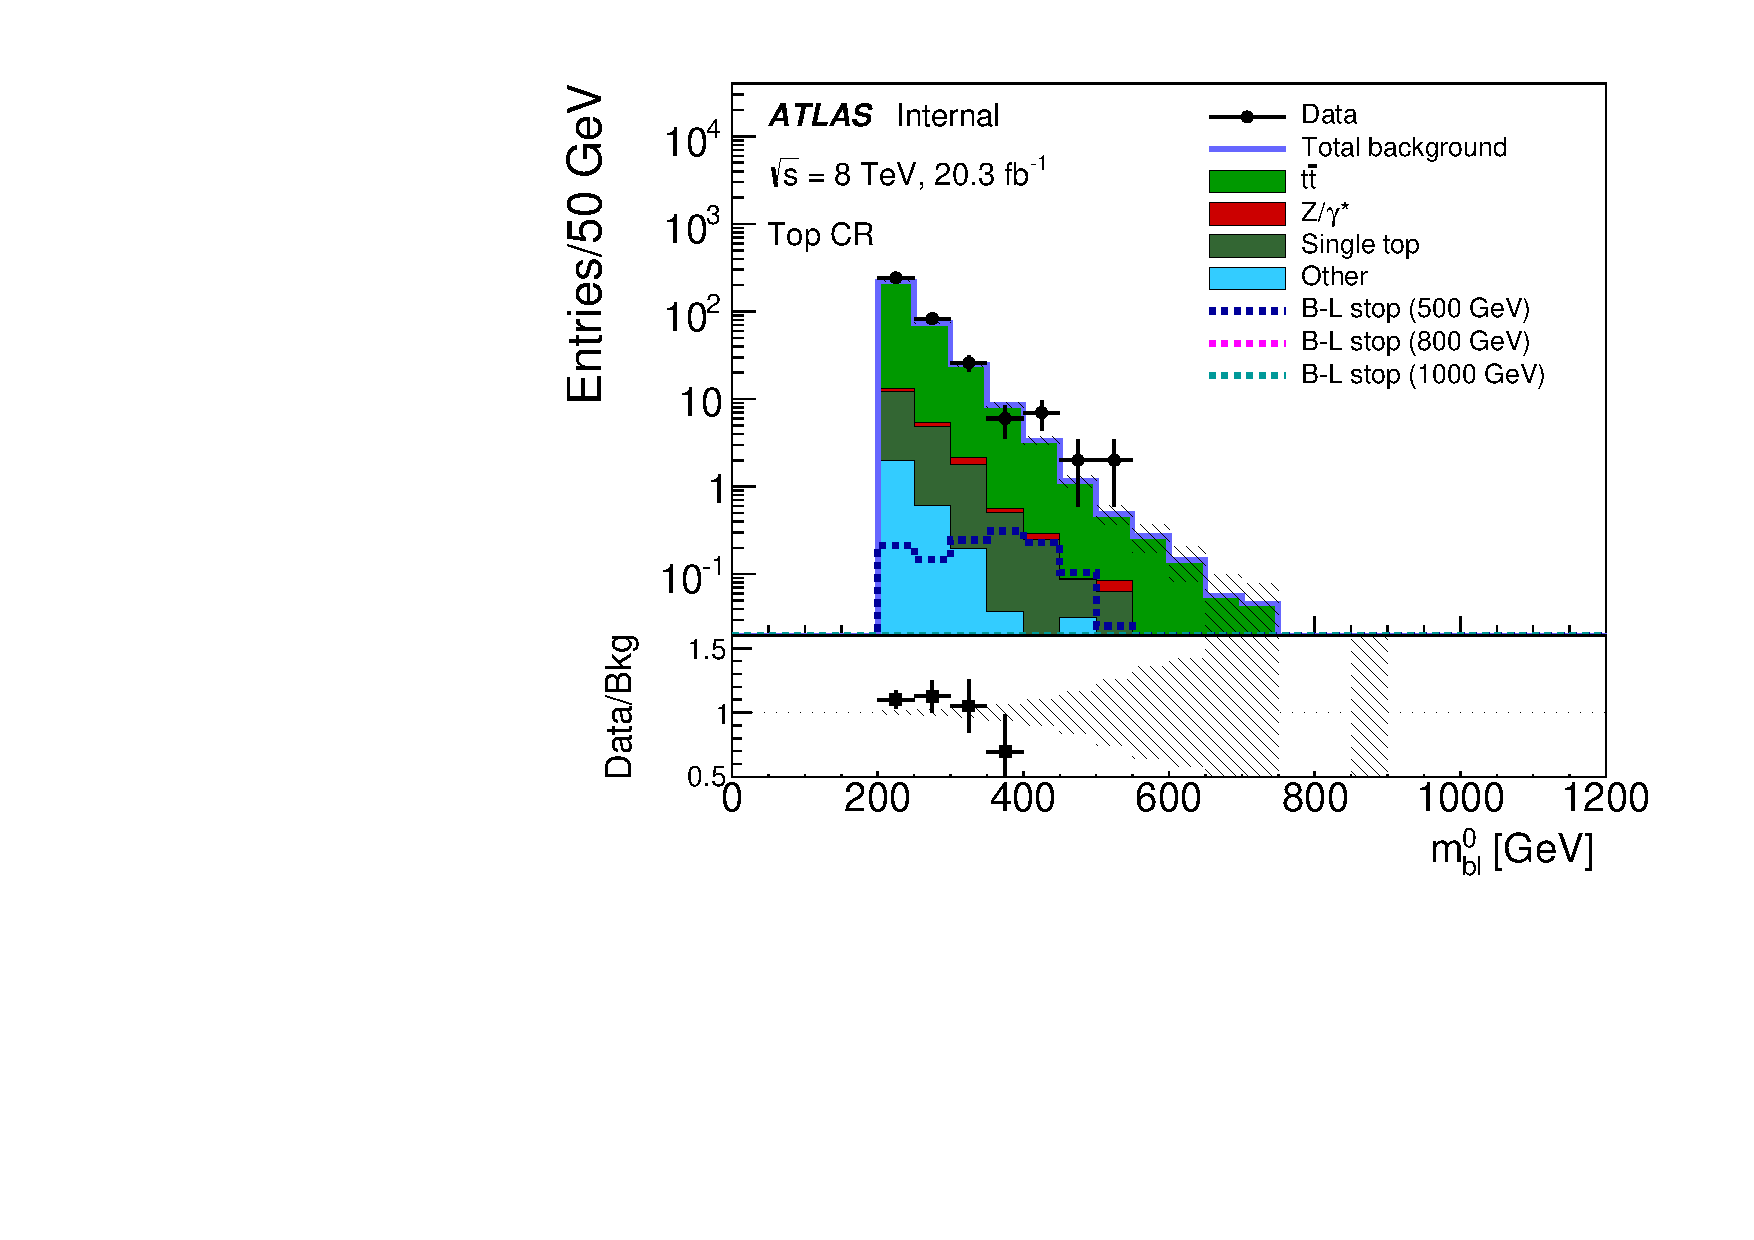
\includegraphics[width=0.48\textwidth, clip=true, trim=0 0 1cm 0]
      {figs/blstop/w_data__no_k_factor__dists/flavor_all__mbl_0__BMINUSL_CR_TOP_MBL_200__log.pdf}
  }
  \subbottom[$Z$ CR]{
    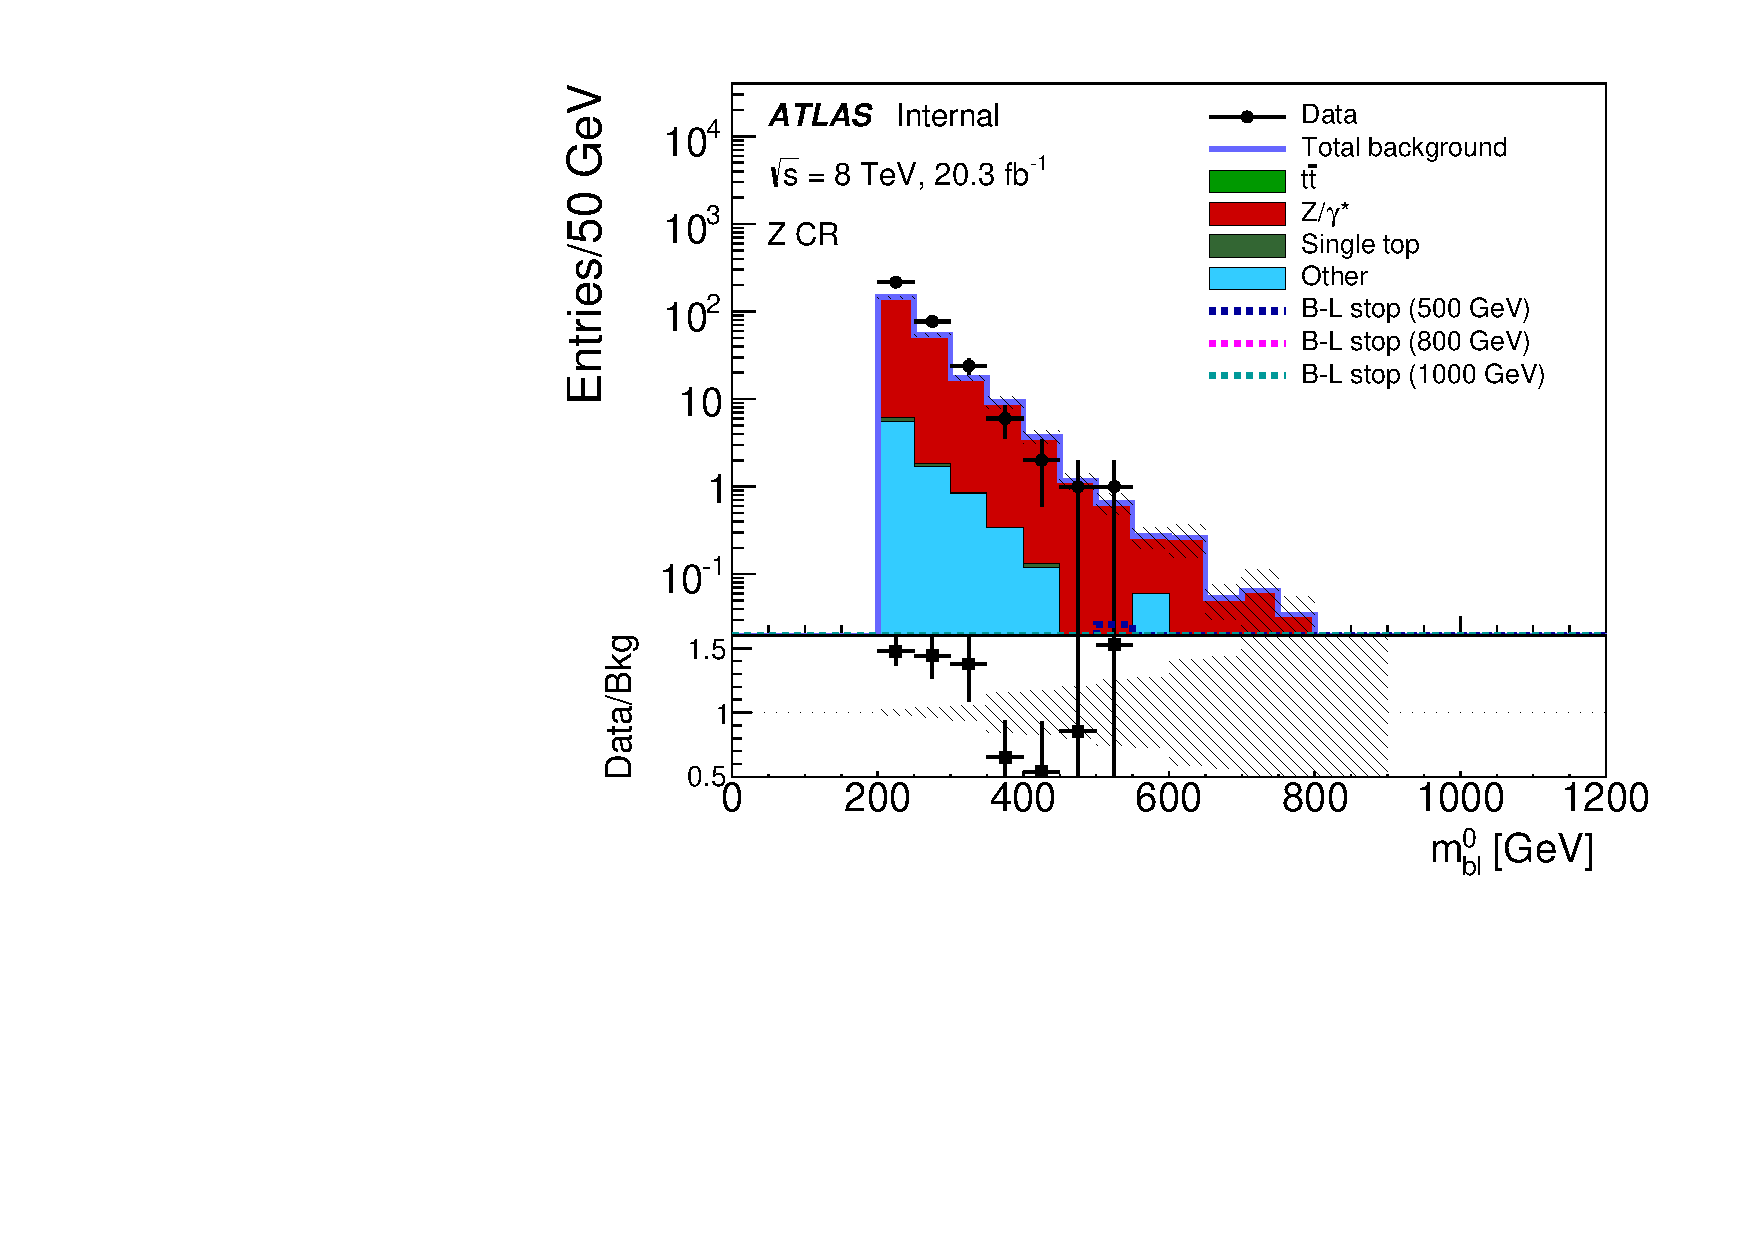
\includegraphics[width=0.48\textwidth, clip=true, trim=0 0 1cm 0]
      {figs/blstop/w_data__no_k_factor__dists/flavor_all__mbl_0__BMINUSL_CR_Z_MBL_200__log.pdf}
  }
  \caption{Expected and observed $\MBL^0$ distribution in the Top CR and
    $Z$ CR when all flavor channels are combined.
    The prediction in the Top CR shows reasonable agreement with the observed
    data.
    The background is underpredicted in the $Z$ CR.
    % In each plot, the last bin includes the overflow for values beyond the
    % maximum shown.
    The hashed error bands show only the statistical uncertainty in the
    background MC simulation samples.
    The signal models have an assumed
    $Br(\tilde{t}\rightarrow be) = Br(\tilde{t}\rightarrow b\mu) = 0.5$.
    {\color{red} TODO remake with dashed line in ratio.}
  }
  \label{fig:cr_mbl_0__no_norm_factor}
  %%
\end{figure}

After applying the $k_Z$ normalization factor the $\MBL^0$ distributions in
the Top CR and $Z$ CR are shown in Figure~\ref{fig:cr_mbl_0__w_norm_factor}.
While the prediction is roughly unchanged in the Top CR, the prediction in the
$Z$ CR shows much better agreement with the data.
The expected and observed event yields in the two CRs, broken out by background
production process, are shown in Table~\ref{tab:region_contributions_cr}.
The expected signal yield in each of the CRs is low, with a signal to
background ratio of less than 0.01.
Additional kinematic distributions including the \pt\ of the leptons and
$b$-jets are shown in
\cref{fig:cr_lep_pt_0__w_norm_factor,fig:cr_lep_pt_1__w_norm_factor,fig:cr_b_jet_pt_0__w_norm_factor,fig:cr_b_jet_pt_1__w_norm_factor}.

\begin{figure}
  \centering
  \subbottom[Top CR]{
    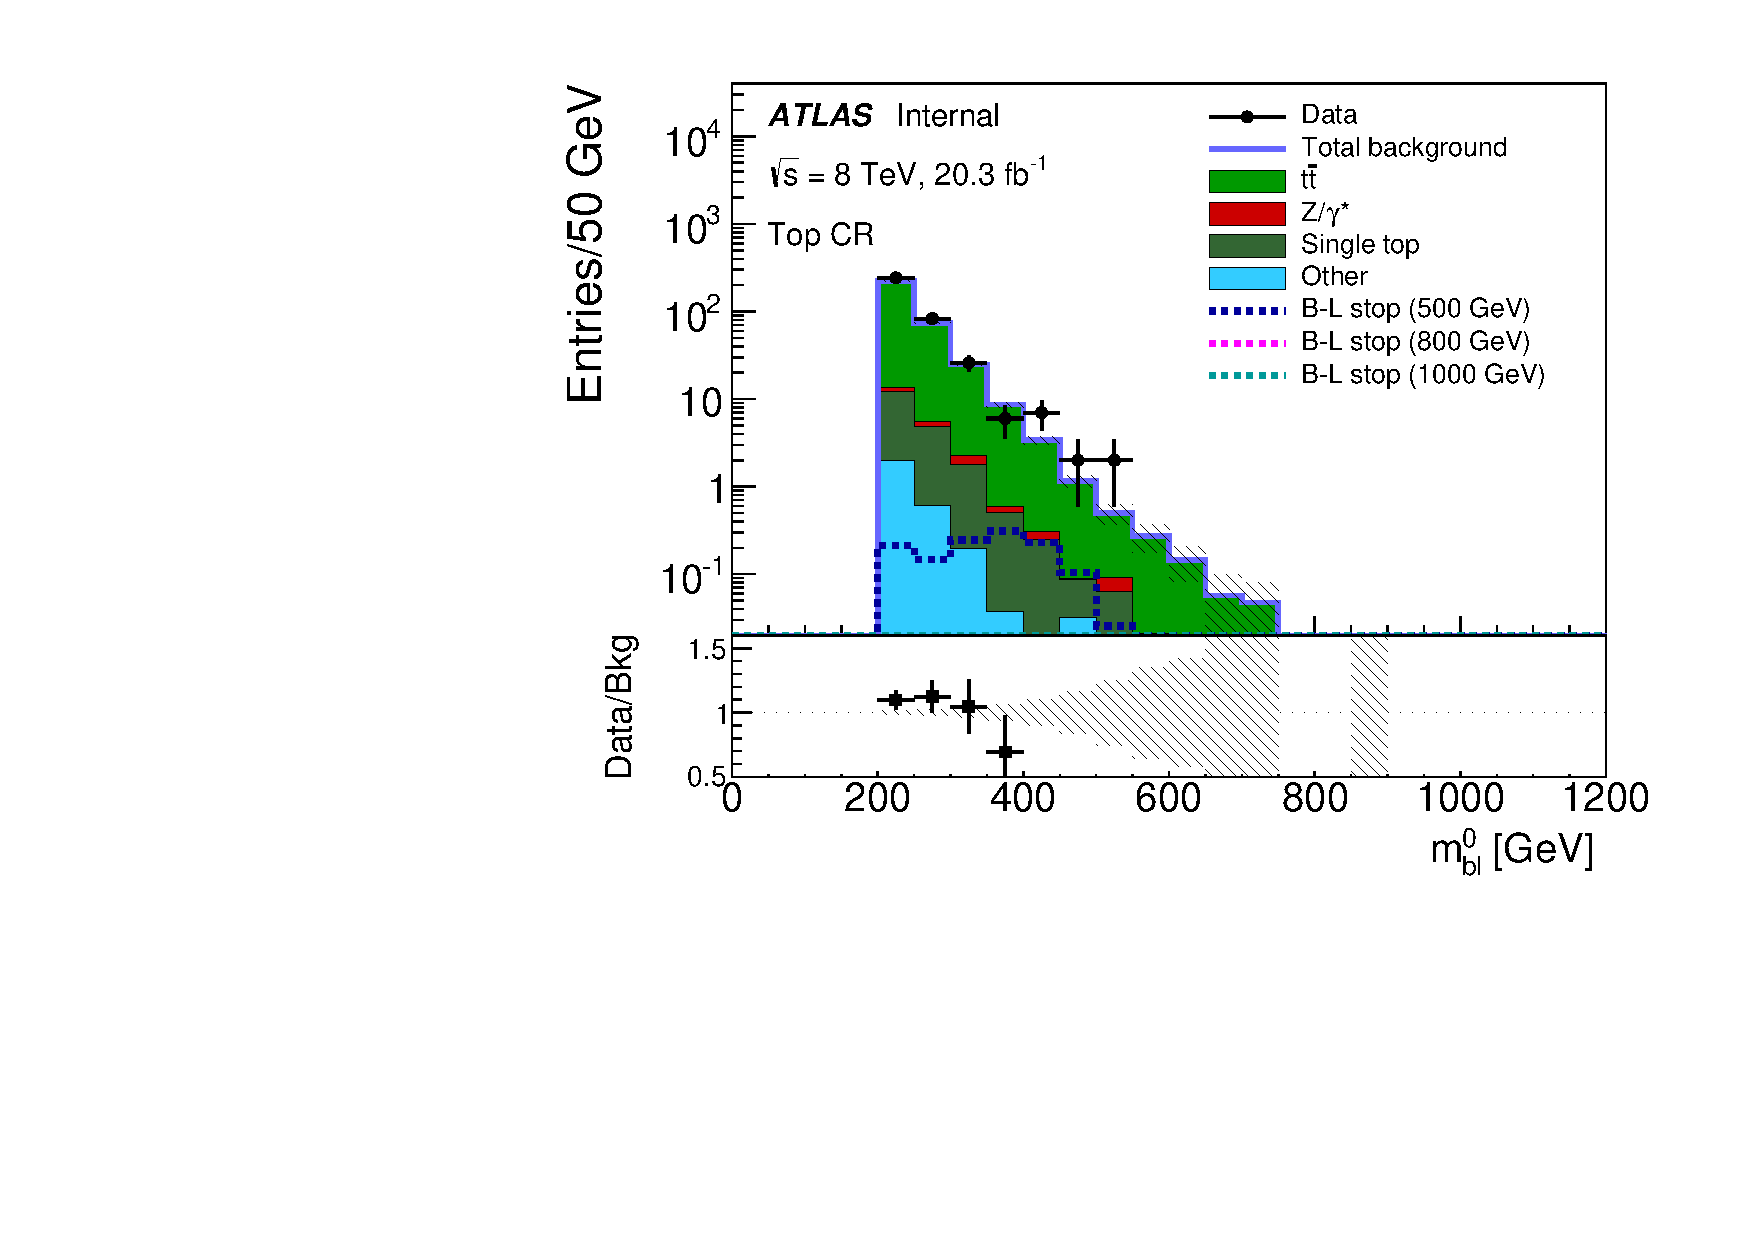
\includegraphics[width=0.48\textwidth, clip=true, trim=0 0 1cm 0]
      {figs/blstop/w_data__w_k_factor__dists/flavor_all__mbl_0__BMINUSL_CR_TOP_MBL_200__log.pdf}
  }
  \subbottom[$Z$ CR]{
    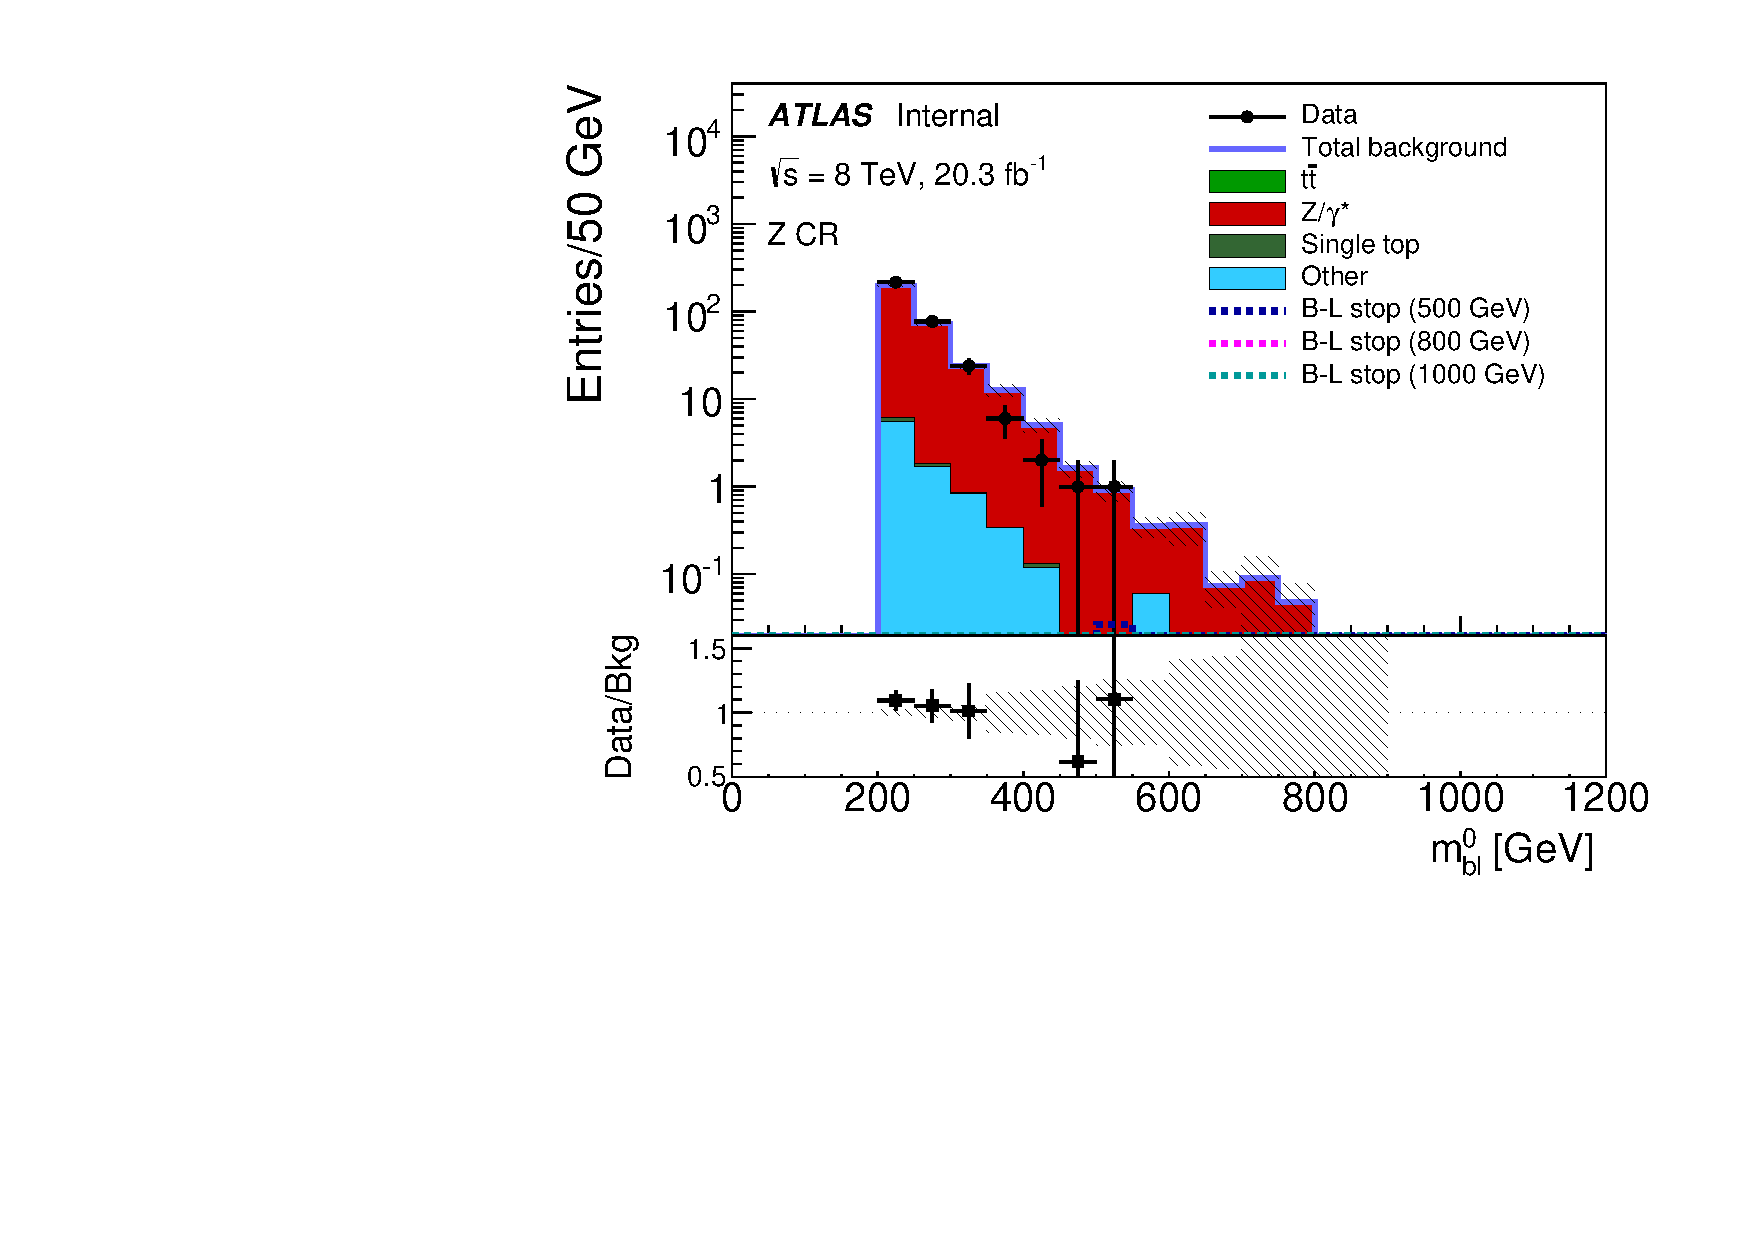
\includegraphics[width=0.48\textwidth, clip=true, trim=0 0 1cm 0]
      {figs/blstop/w_data__w_k_factor__dists/flavor_all__mbl_0__BMINUSL_CR_Z_MBL_200__log.pdf}
  }
  \caption{Expected and observed $\MBL^0$ distribution in the Top CR and
    $Z$ CR after applying the $k_Z$ normalization factor derived in the $Z$ CR
    when all flavor channels are combined.
    After applying the $k_Z$ normalization factor, both CRs show reasonable
    agreement between the predicted and observed distributions.
    % In each plot, the last bin includes the overflow for values beyond the
    % maximum shown.
    The hashed error bands show only the statistical uncertainty in the
    background MC simulation samples.
    The signal models have an assumed
    $Br(\tilde{t}\rightarrow be) = Br(\tilde{t}\rightarrow b\mu) = 0.5$.
    {\color{red} TODO remake with dashed line in ratio.}
  }
  \label{fig:cr_mbl_0__w_norm_factor}
  %%
\end{figure}

\begin{figure}
  \centering
  \subbottom[Top CR]{
    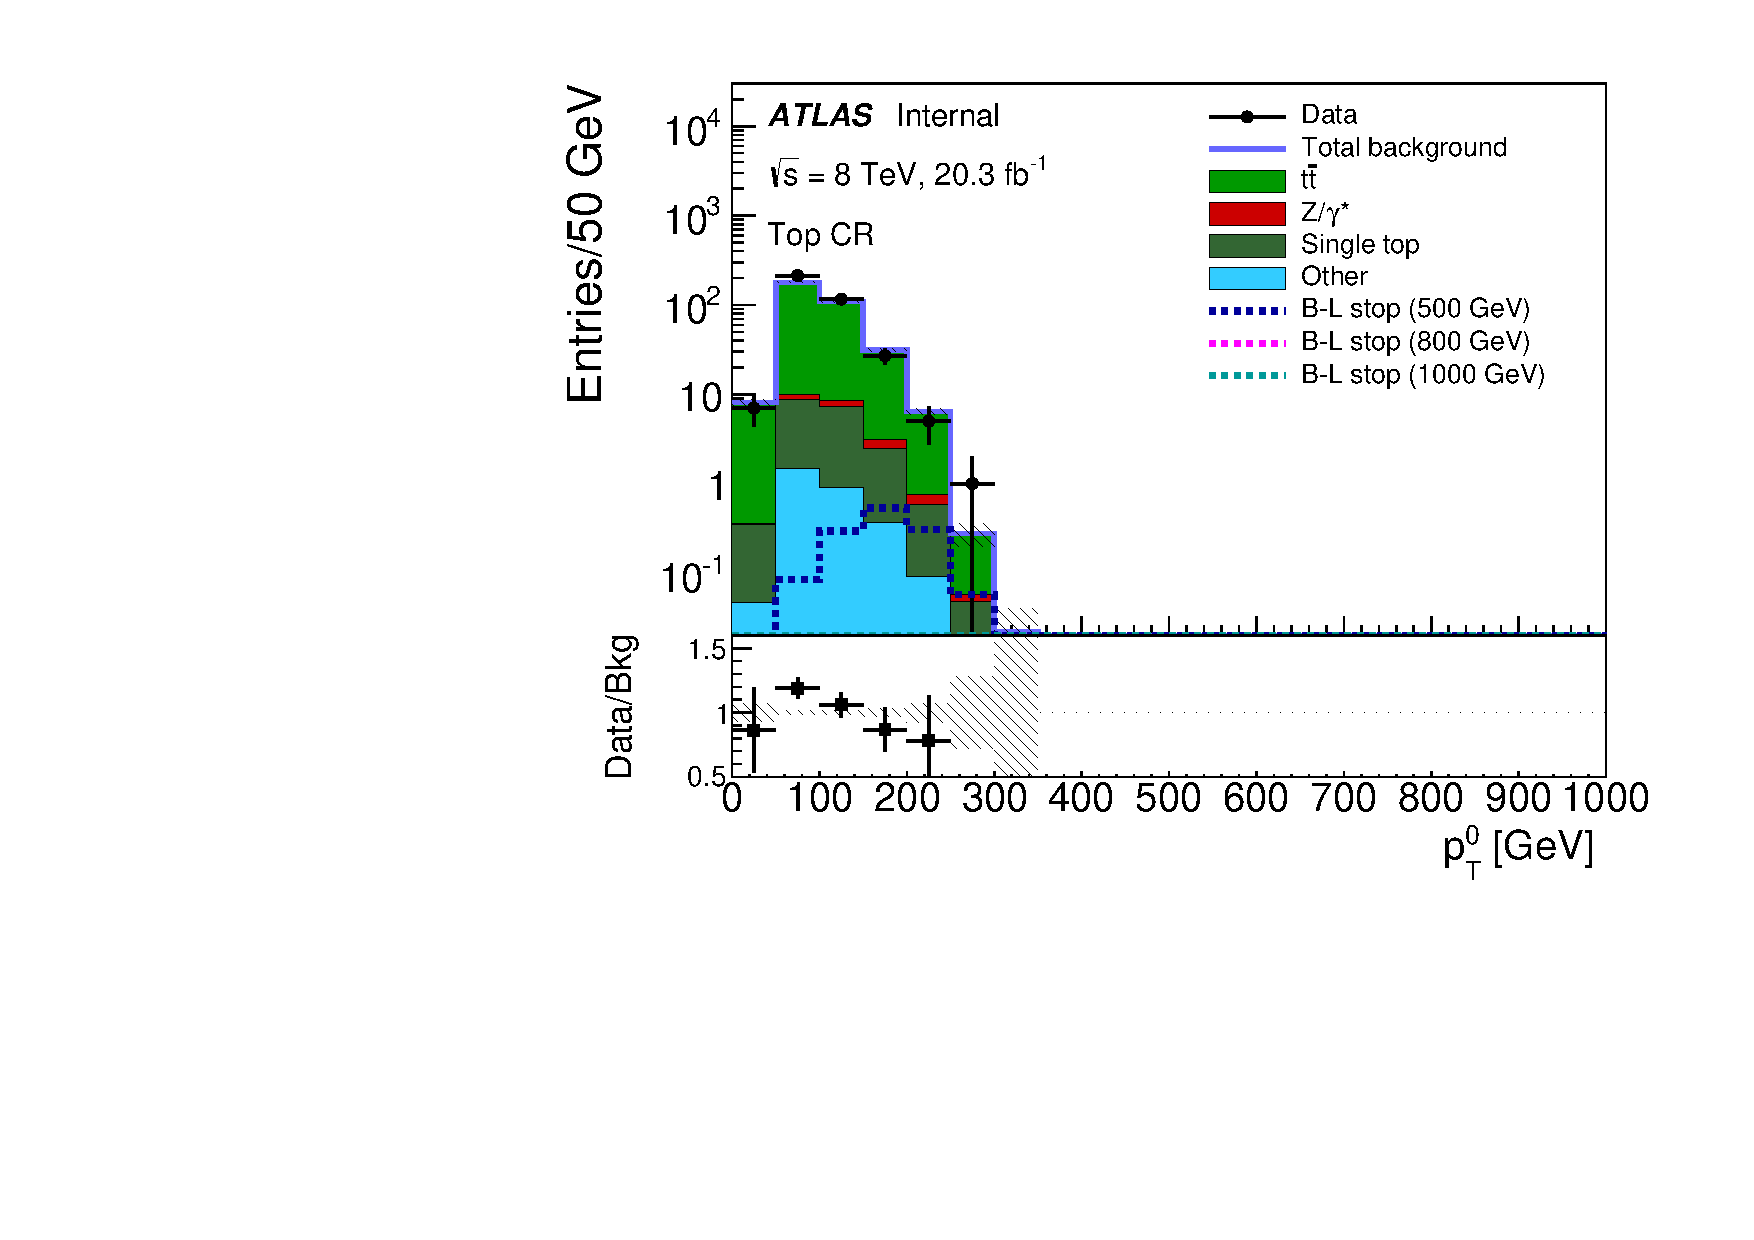
\includegraphics[width=0.48\textwidth, clip=true, trim=0 0 1cm 0]
      {figs/blstop/w_data__w_k_factor__dists/flavor_all__lep_pt_0__BMINUSL_CR_TOP_MBL_200__log.pdf}
  }
  \subbottom[$Z$ CR]{
    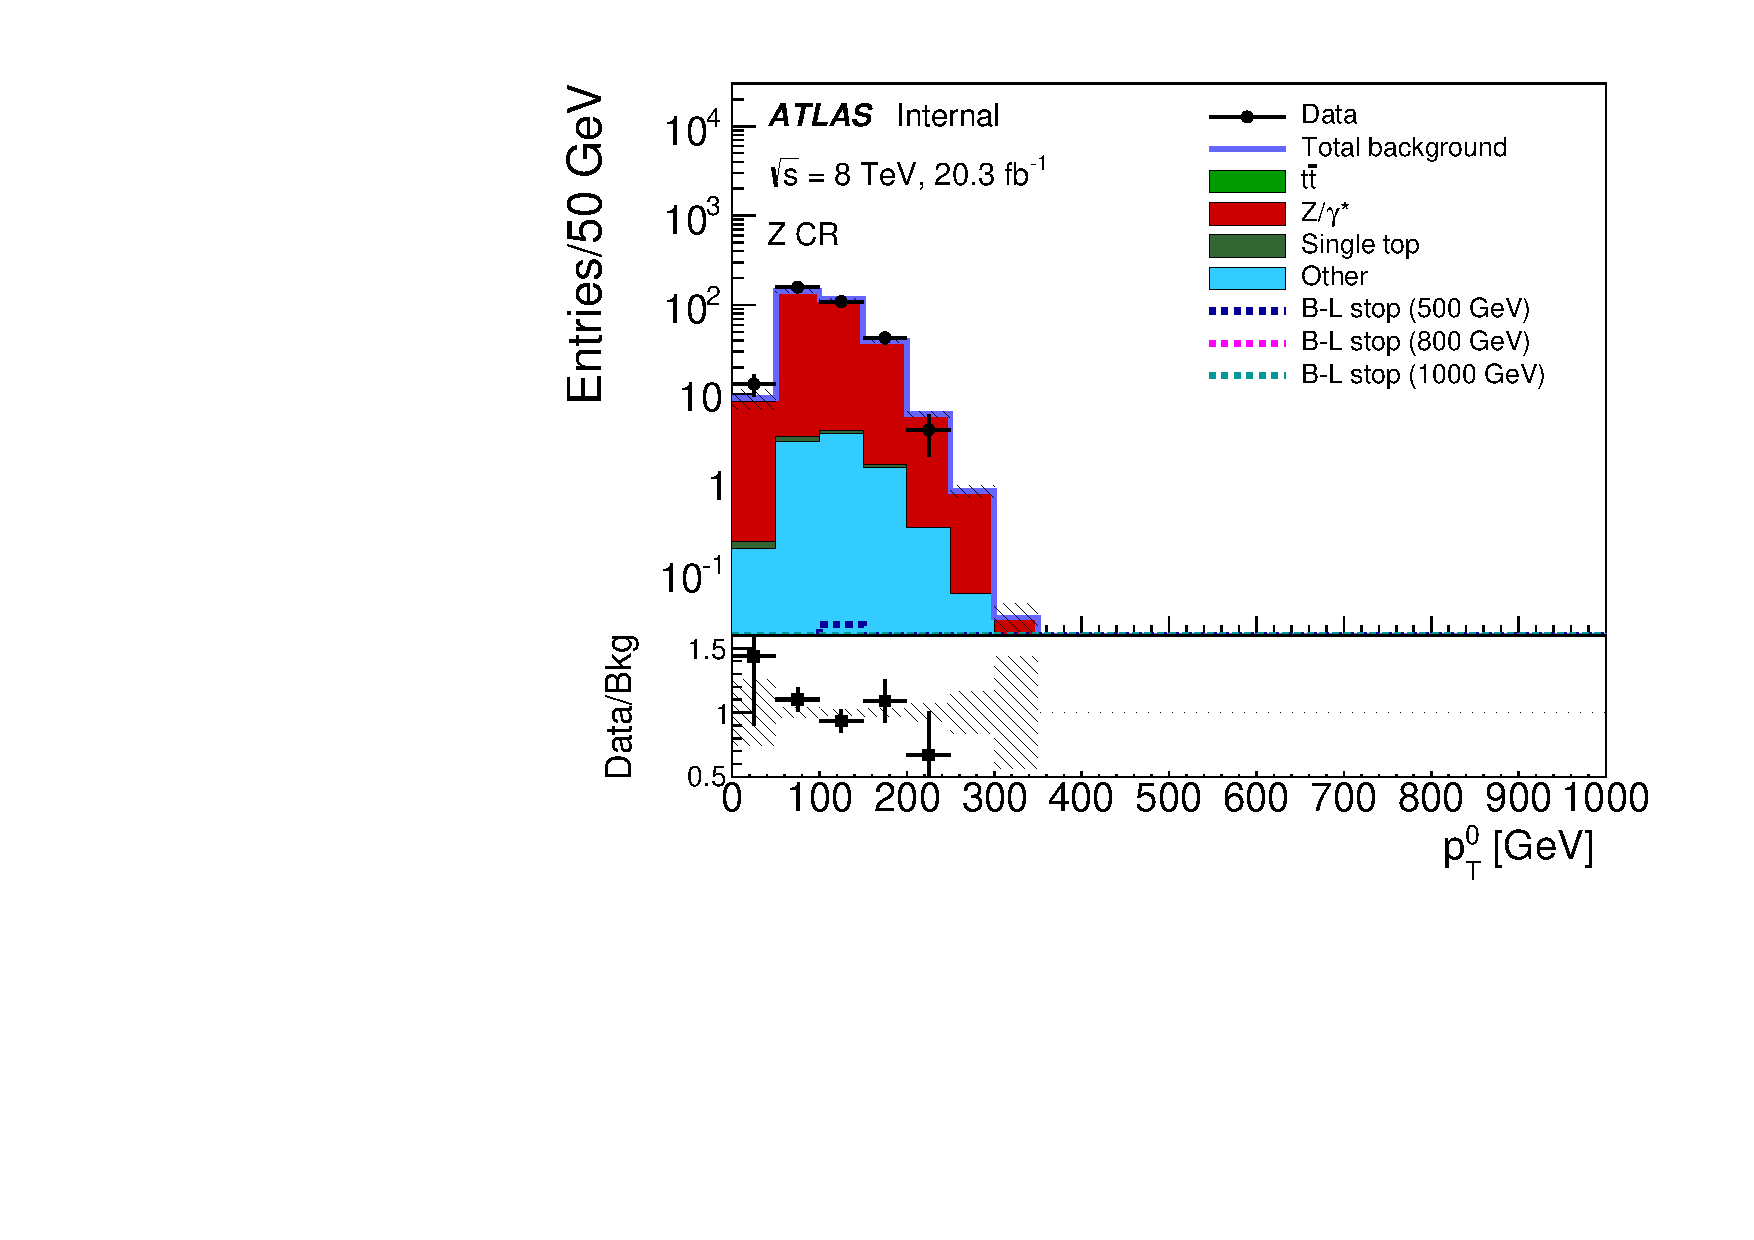
\includegraphics[width=0.48\textwidth, clip=true, trim=0 0 1cm 0]
      {figs/blstop/w_data__w_k_factor__dists/flavor_all__lep_pt_0__BMINUSL_CR_Z_MBL_200__log.pdf}
  }
  \caption{Expected and observed \pt\ distribution for the leading lepton in
    the Top CR and $Z$ CR after applying the $k_Z$ normalization factor derived
    in the $Z$ CR when all flavor channels are combined.
    % After applying the $k_Z$ normalization factor, both CRs show reasonable
    % agreement between the predicted and observed distributions.
    % In each plot, the last bin includes the overflow for values beyond the
    % maximum shown.
    The hashed error bands show only the statistical uncertainty in the
    background MC simulation samples.
    The signal models have an assumed
    $Br(\tilde{t}\rightarrow be) = Br(\tilde{t}\rightarrow b\mu) = 0.5$.
    {\color{red} TODO remake with dashed line in ratio.}
  }
  \label{fig:cr_lep_pt_0__w_norm_factor}
  %%
\end{figure}

\begin{figure}
  \centering
  \subbottom[Top CR]{
    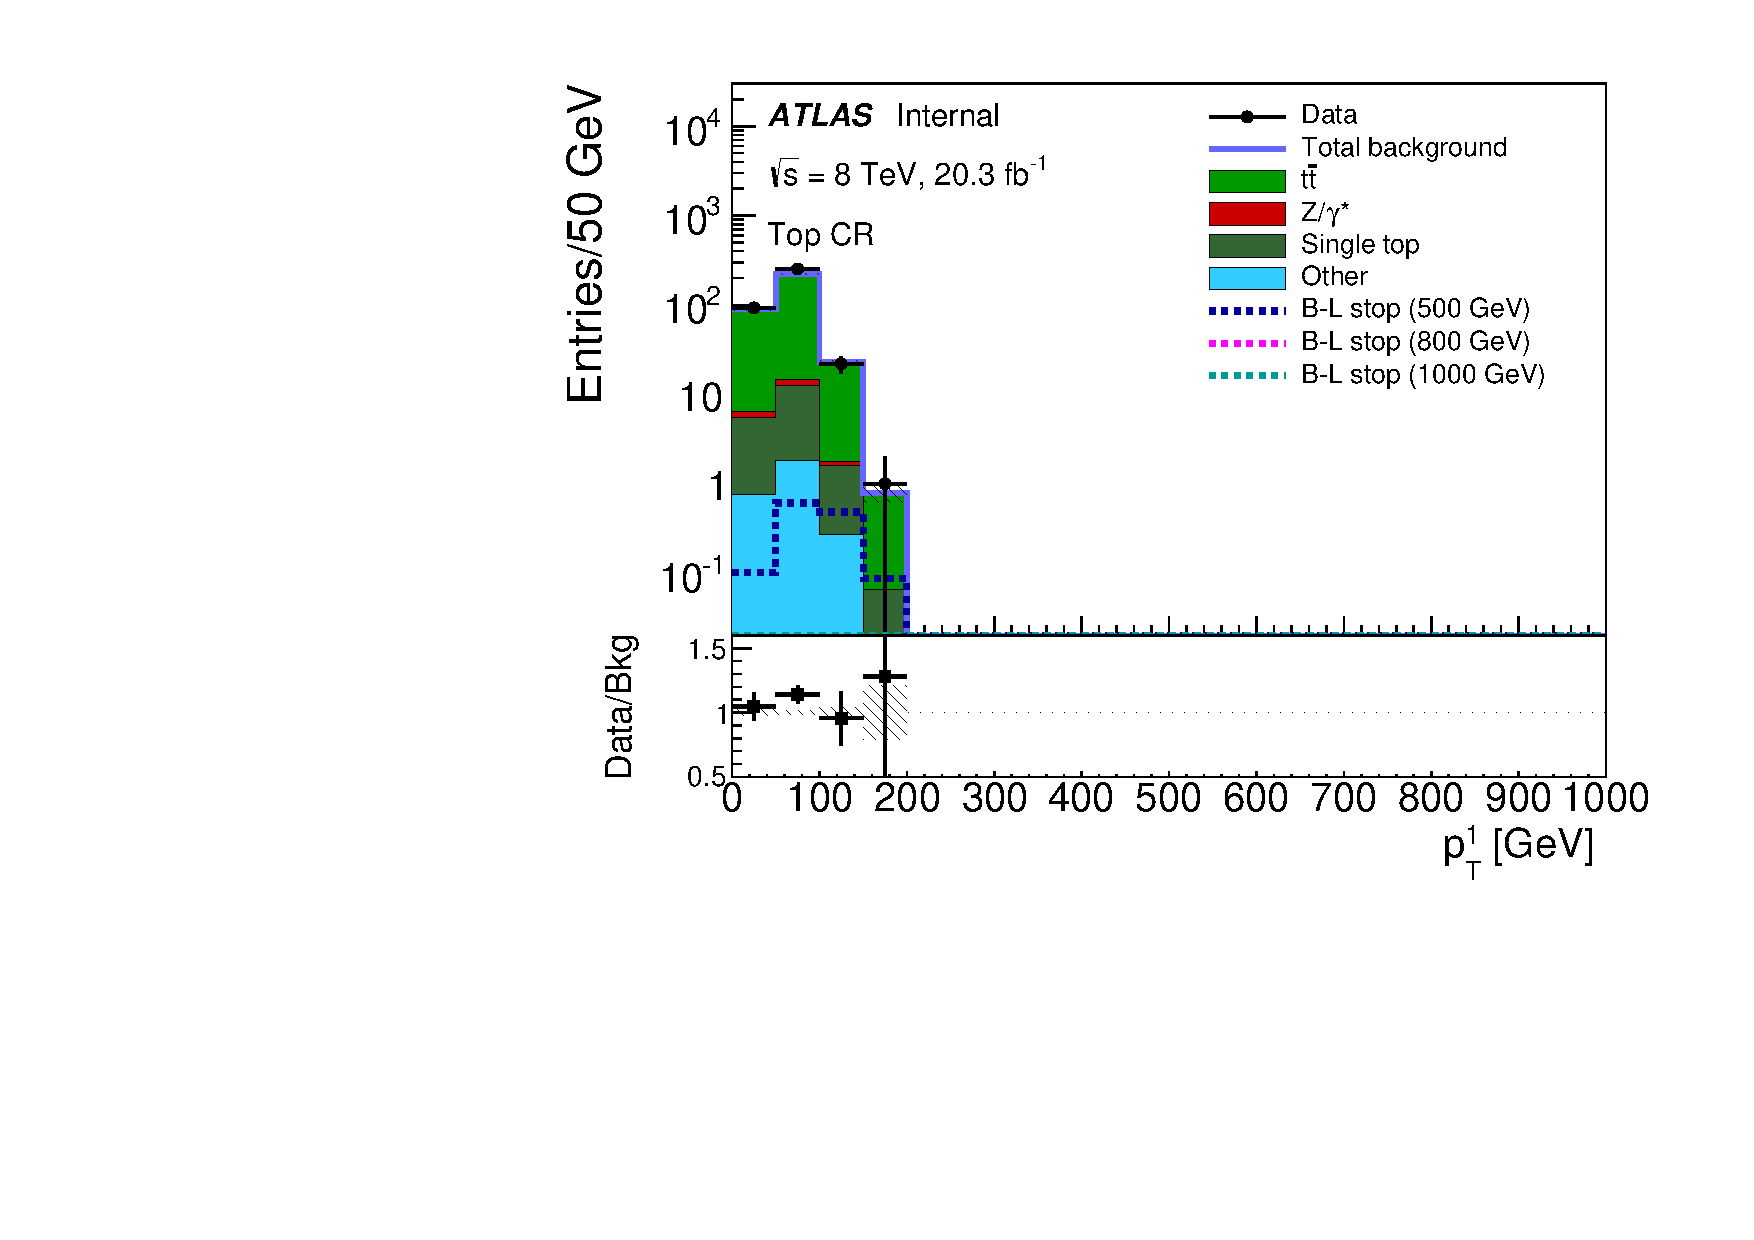
\includegraphics[width=0.48\textwidth, clip=true, trim=0 0 1cm 0]
      {figs/blstop/w_data__w_k_factor__dists/flavor_all__lep_pt_1__BMINUSL_CR_TOP_MBL_200__log.pdf}
  }
  \subbottom[$Z$ CR]{
    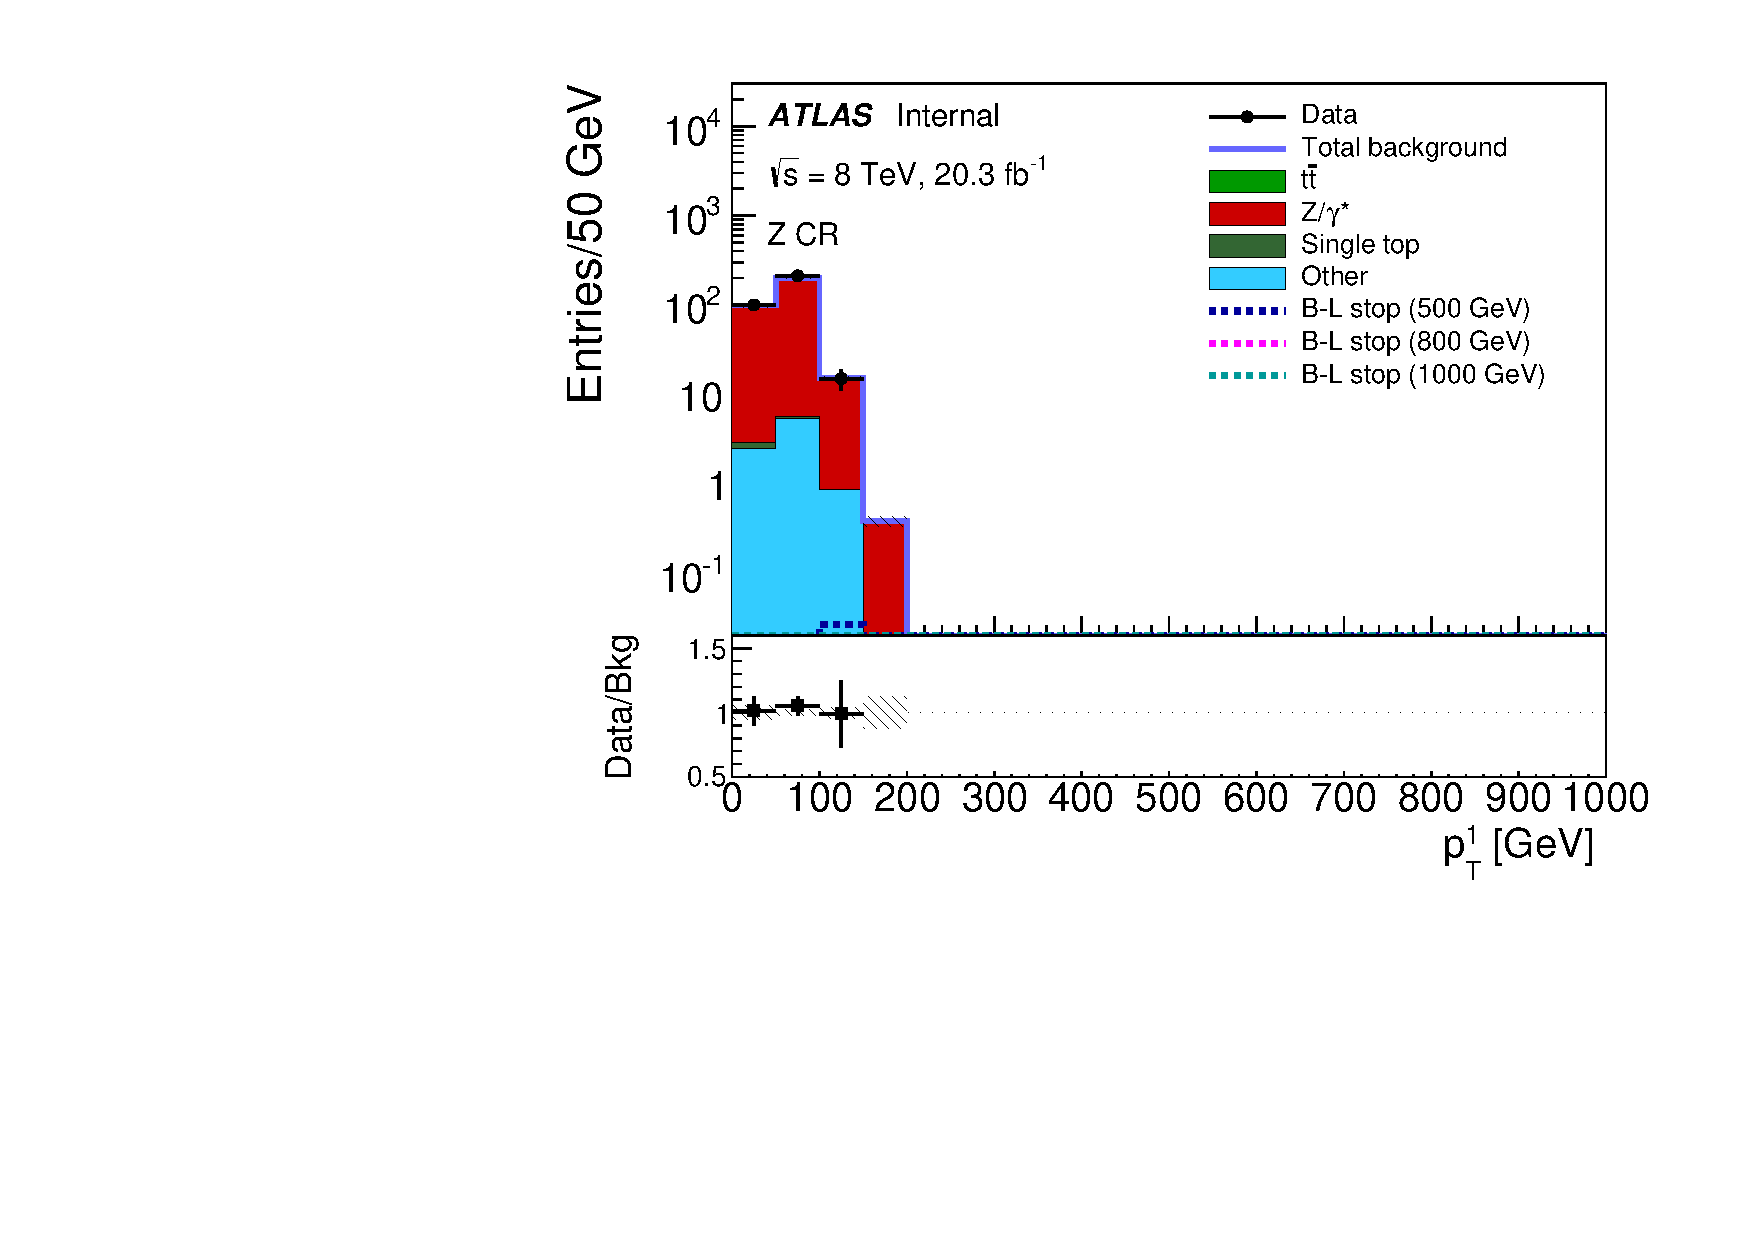
\includegraphics[width=0.48\textwidth, clip=true, trim=0 0 1cm 0]
      {figs/blstop/w_data__w_k_factor__dists/flavor_all__lep_pt_1__BMINUSL_CR_Z_MBL_200__log.pdf}
  }
  \caption{Expected and observed \pt\ distribution for the sub-leading lepton in
    the Top CR and $Z$ CR after applying the $k_Z$ normalization factor derived
    in the $Z$ CR when all flavor channels are combined.
    % After applying the $k_Z$ normalization factor, both CRs show reasonable
    % agreement between the predicted and observed distributions.
    % In each plot, the last bin includes the overflow for values beyond the
    % maximum shown.
    The hashed error bands show only the statistical uncertainty in the
    background MC simulation samples.
    The signal models have an assumed
    $Br(\tilde{t}\rightarrow be) = Br(\tilde{t}\rightarrow b\mu) = 0.5$.
    {\color{red} TODO remake with dashed line in ratio.}
  }
  \label{fig:cr_lep_pt_1__w_norm_factor}
  %%
\end{figure}

\begin{figure}
  \centering
  \subbottom[Top CR]{
    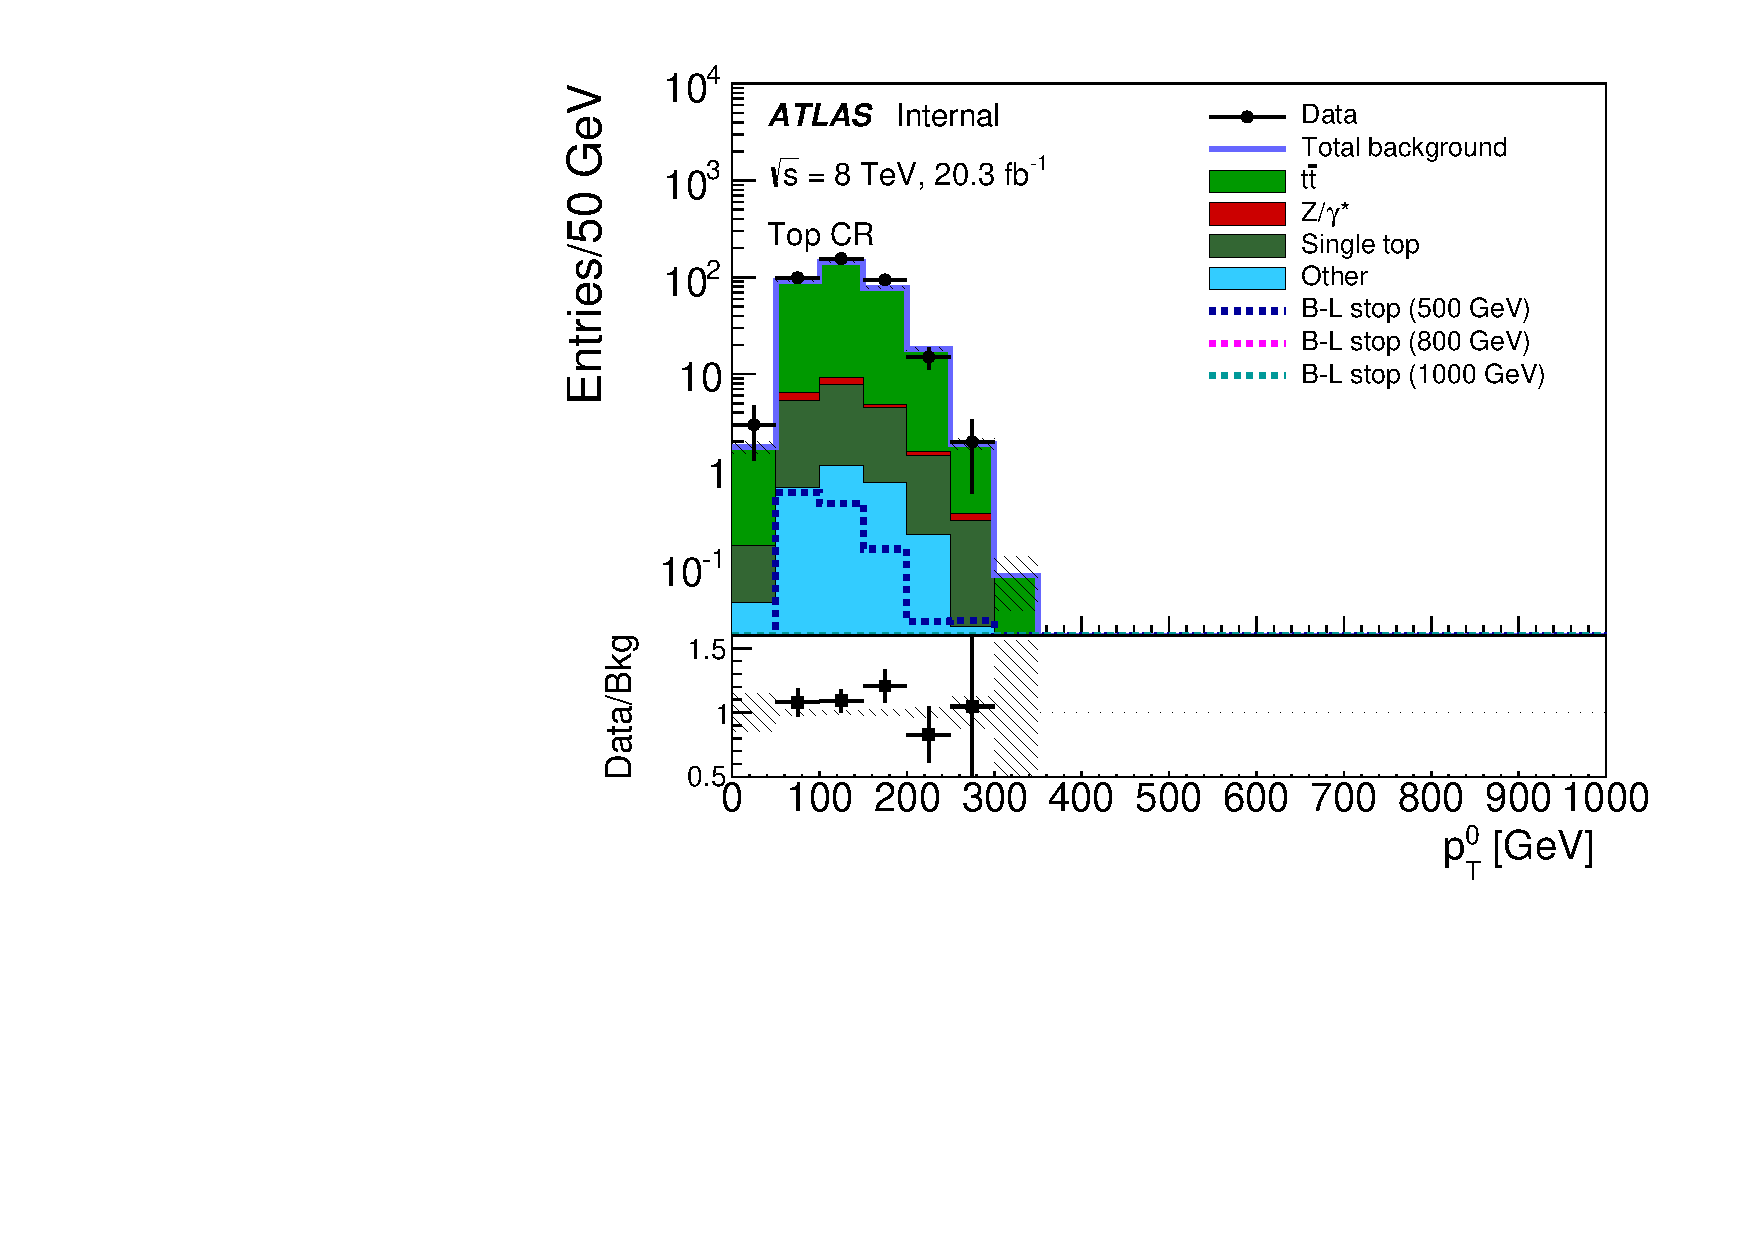
\includegraphics[width=0.48\textwidth, clip=true, trim=0 0 1cm 0]
      {figs/blstop/w_data__w_k_factor__dists/flavor_all__b_jet_pt_0__BMINUSL_CR_TOP_MBL_200__log.pdf}
  }
  \subbottom[$Z$ CR]{
    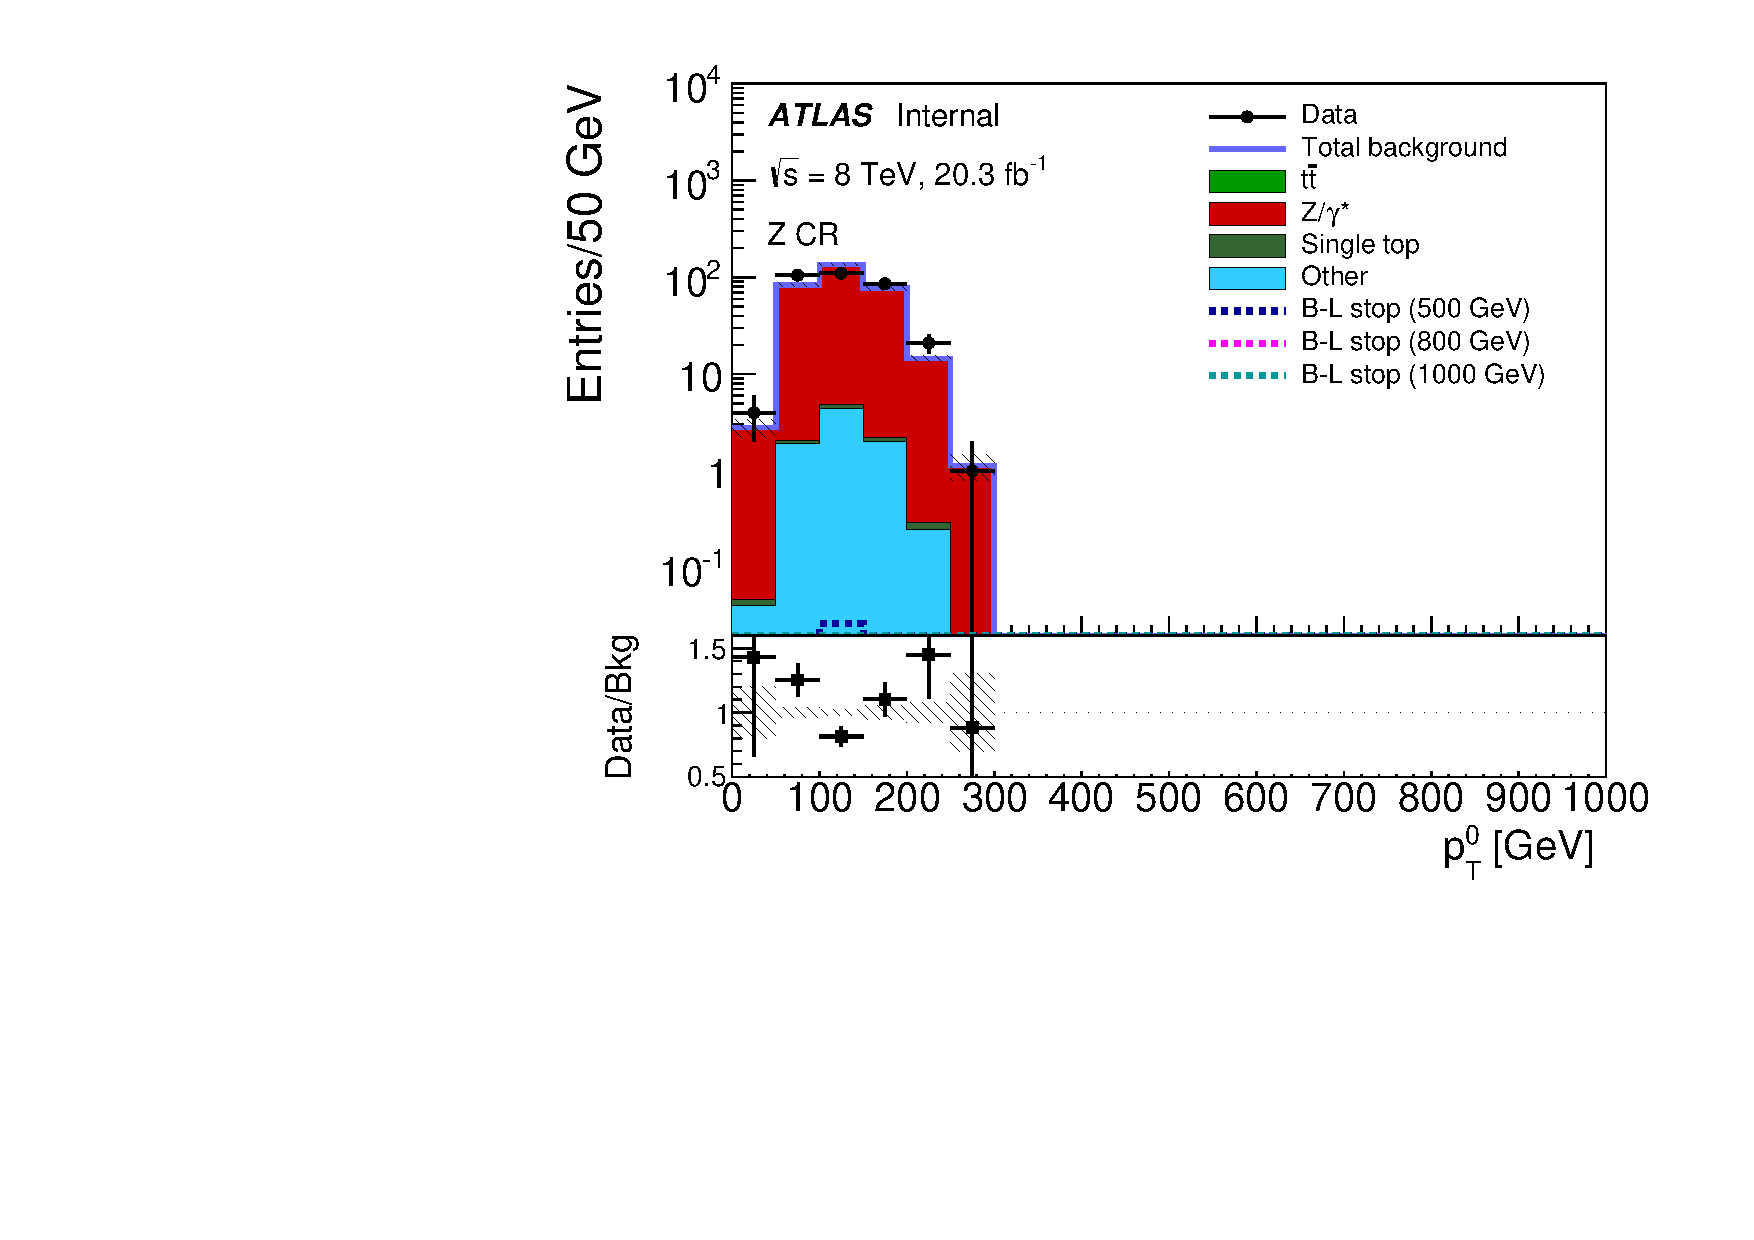
\includegraphics[width=0.48\textwidth, clip=true, trim=0 0 1cm 0]
      {figs/blstop/w_data__w_k_factor__dists/flavor_all__b_jet_pt_0__BMINUSL_CR_Z_MBL_200__log.pdf}
  }
  \caption{Expected and observed \pt\ distribution for the leading $b$-jet in
    the Top CR and $Z$ CR after applying the $k_Z$ normalization factor derived
    in the $Z$ CR when all flavor channels are combined.
    % After applying the $k_Z$ normalization factor, both CRs show reasonable
    % agreement between the predicted and observed distributions.
    % In each plot, the last bin includes the overflow for values beyond the
    % maximum shown.
    The hashed error bands show only the statistical uncertainty in the
    background MC simulation samples.
    The signal models have an assumed
    $Br(\tilde{t}\rightarrow be) = Br(\tilde{t}\rightarrow b\mu) = 0.5$.
    {\color{red} TODO remake with dashed line in ratio.}
  }
  \label{fig:cr_b_jet_pt_0__w_norm_factor}
  %%
\end{figure}

\begin{figure}
  \centering
  \subbottom[Top CR]{
    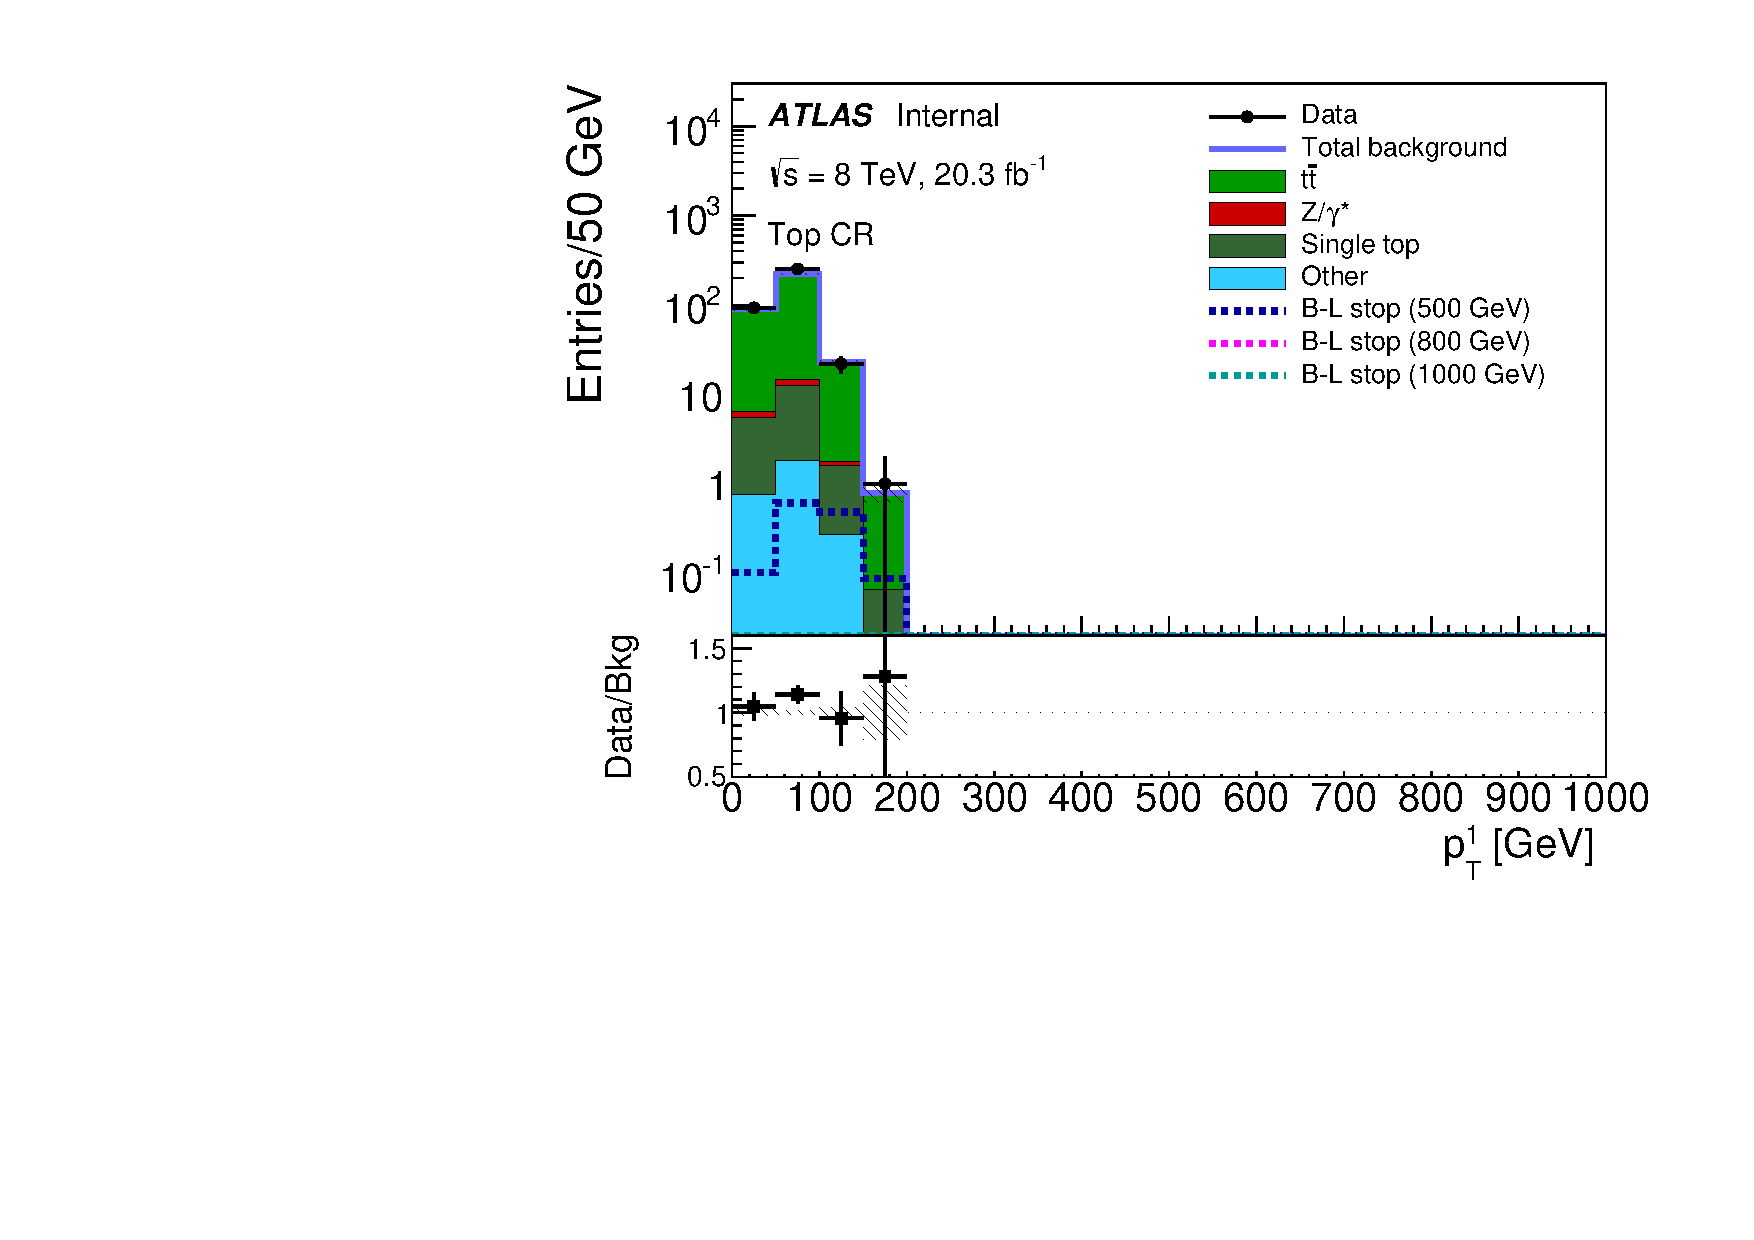
\includegraphics[width=0.48\textwidth, clip=true, trim=0 0 1cm 0]
      {figs/blstop/w_data__w_k_factor__dists/flavor_all__lep_pt_1__BMINUSL_CR_TOP_MBL_200__log.pdf}
  }
  \subbottom[$Z$ CR]{
    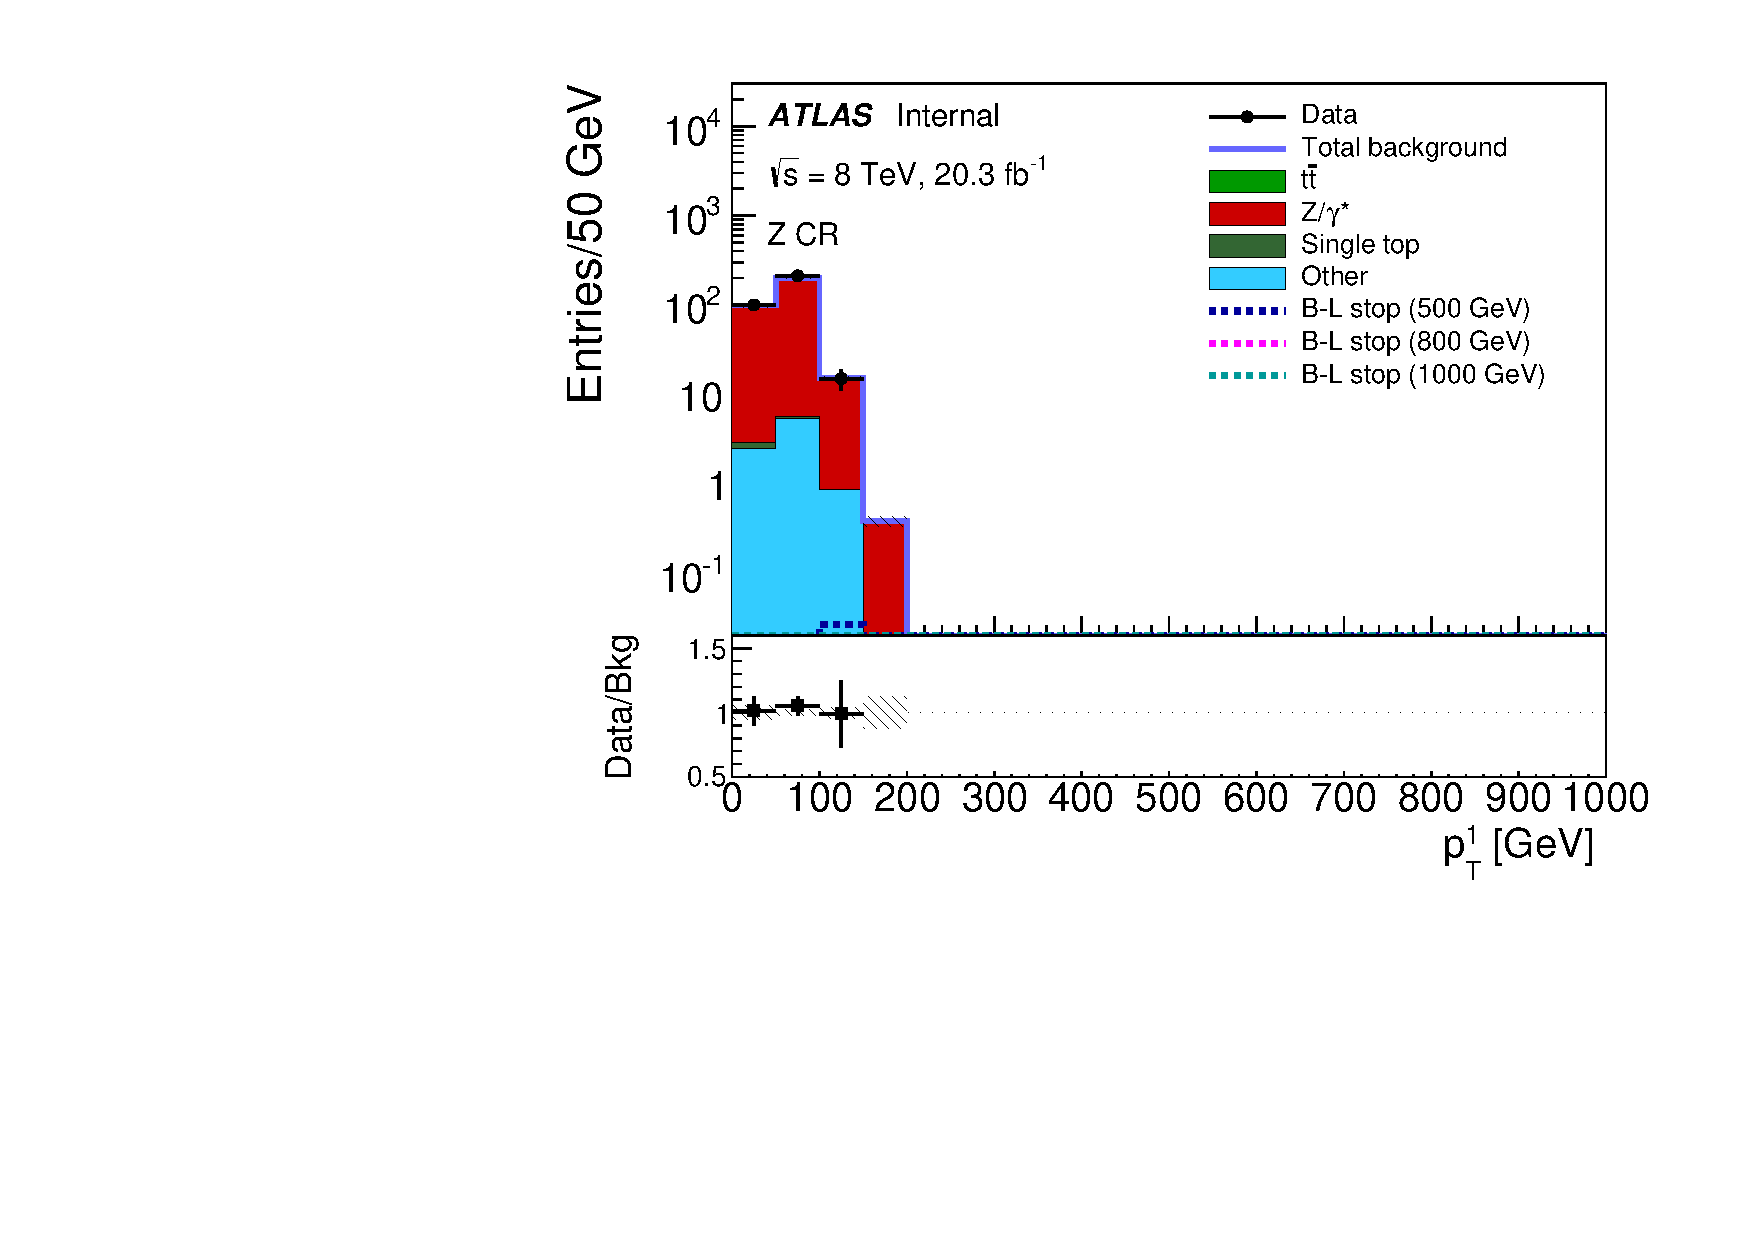
\includegraphics[width=0.48\textwidth, clip=true, trim=0 0 1cm 0]
      {figs/blstop/w_data__w_k_factor__dists/flavor_all__lep_pt_1__BMINUSL_CR_Z_MBL_200__log.pdf}
  }
  \caption{Expected and observed \pt\ distribution for the sub-leading $b$-jet
    in the Top CR and $Z$ CR after applying the $k_Z$ normalization factor
    derived in the $Z$ CR when all flavor channels are combined.
    % After applying the $k_Z$ normalization factor, both CRs show reasonable
    % agreement between the predicted and observed distributions.
    % In each plot, the last bin includes the overflow for values beyond the
    % maximum shown.
    The hashed error bands show only the statistical uncertainty in the
    background MC simulation samples.
    The signal models have an assumed
    $Br(\tilde{t}\rightarrow be) = Br(\tilde{t}\rightarrow b\mu) = 0.5$.
    {\color{red} TODO remake with dashed line in ratio.}
  }
  \label{fig:cr_b_jet_pt_1__w_norm_factor}
  %%
\end{figure}

\begin{table}
  \caption{Number of expected events in each of the CRs broken down by process.
    The uncertainty in the total background prediction is the MC statistical
    uncertainty only for each background process.
    The total uncertainty is obtained by summing the uncertainty in each
    background process in quadrature.
    The $k_Z$ normalization factor is applied to the \ZGAMMAJETS\ background
    yield estimate.
    For each signal model, the expected signal to background ratio is given in
    parentheses.
    % For each signal model, the ratio of expected signal events to the sum of the
    % background in each region is show in parentheses.
    {\color{red} TODO add observed number events in each CR.}
    {\color{red} TODO update with only stat uncertainty.}
    {\color{red} TODO update with breakdown by flavor channel.}
  }
  \label{tab:region_contributions_cr}
  \centering{
    \begin{tabular}{c|cc}
      \toprule
                                           & Top CR                            & $Z$ CR                            \\
      \midrule
      \TTBAR                               & $311.8$                           & $8.2$                             \\
      \ZGAMMAJETS                          & $3.1$                             & $297.9$                           \\
      Single top                           & $16.7$                            & $0.8$                             \\
      Other                                & $2.9$                             & $8.6$                             \\
      \midrule
      Total                                & \multirow{2}{*}{$334.5 \pm 93.7$} & \multirow{2}{*}{$315.6 \pm 89.5$} \\
      background                           &                                   &                                   \\
      \midrule
      \multirow{2}{*}{B-L stop (500 GeV)}  & $1.3$                             & $0.03$                            \\
                                           & ($< 0.01$)                        & ($< 0.01$) \vspace{1ex}           \\
      \multirow{2}{*}{B-L stop (800 GeV)}  & $< 0.01$                          & $< 0.01$                          \\
                                           & ($< 0.01$)                        & ($< 0.01$) \vspace{1ex}           \\
      \multirow{2}{*}{B-L stop (1000 GeV)} & $< 0.01$                          & $< 0.01$                          \\
                                           & ($< 0.01$)                        & ($< 0.01$) \vspace{1ex}           \\
      \bottomrule
    \end{tabular}
  }
\end{table}

%% -----------------------------------------------------------------------------
\FloatBarrier
\subsection{Validation regions}
\label{sec:vr}

The normalization factors for the \TTBAR\ and \ZGAMMAJETS\ background processes
are determined using the observed data in the CRs, then used to estimate the
background contribution in the SRs.
To show these normalization factors are valid in regions of kinematic space away
from the CRs, Validation regions (VRs), which are orthogonal to the CRs and SRs
are defined, where the background prediction can be compared with the
observation.
These VRs should have low expected signal contamination, but do not need to be
pure in any particular background process, as is required of the CRs.
Since this analysis targets stops with reasonably high mass, all VRs require
$\MBL^0 \geq 200 \GeV$ as is required in the CRs.
As with the CRs, regions with higher \MBL\ requires were tested, but the
expected and observed event yields were too low to make a reliable comparison.

As shown in Figure~\ref{fig:region_coverage} and Table~\ref{tab:regions},
three orthogonal VRs are defined to validate the \TTBAR\ background estimate,
labeled Top VR 1, Top VR 2, and Top VR 3.
Top VR 1 is constructed by reversing the cut on \METSIG\ in the Top CR.
That is, Top VR 1 requires events have $\METSIG < 4 \GeV^{1/2}$, and is
otherwise identical to the Top CR.
Top VR 2 is obtained by reversing the \MBLASYM\ requirement in the Top CR and
relaxing the \METSIG\ requirement.
Top VR 3 is intended to validate the extrapolation of the \TTBAR\ background
prediction from the low \HT\ Top CR to the high \HT\ region of the SRs.
The Top VR 3 region is obtained by reversing the \HT\ selection criteria from
the Top VR 2 region, giving a region with $\MBLASYM > 0.2$ and $\HT > 500 \GeV$.

The $Z$ VR is used to validate the extrapolation of the \ZGAMMAJETS\ background
prediction from the $Z$ CR to kinematic regions higher \HT.
This region is constructed by reversing the \HT\ selection criteria from the
$Z$ CR, and relaxing the \METSIG\ requirement.
The full VR selection criteria are outlined along with the other analysis
regions in Table~\ref{tab:regions} and Figure~\ref{fig:region_coverage}.
The expected and observed event yields in the VRs, broken out by background
production process, are shown in Table~\ref{tab:region_contributions_vr}.
Select kinematic distributions in the VRs are shown in
Figure~\ref{fig:vr_dists_w_norm_factor}.
The agreement between the observed and predicted yields and distributions in the
VRs is explored in more detail in Section~\ref{sec:bkg_fit}.

\begin{table}
  \caption{Number of expected events in each of the VRs broken down by process.
    The uncertainty in the total background prediction is the MC statistical
    uncertainty only for each background process.
    The total uncertainty is obtained by summing the uncertainty in each
    background process in quadrature.
    The $k_Z$ normalization factor is applied to the \ZGAMMAJETS\ background
    yield estimate.
    For each signal model, the ratio of expected signal events to the sum of the
    background in each region is show in parentheses.
    {\color{red} TODO add observed number events in each VR.}
    {\color{red} TODO update with only stat uncertainty.}
    {\color{red} TODO update with breakdown by flavor channel.}
  }
  \label{tab:region_contributions_vr}
  \centering{
    \begin{tabular}{c|cccc}
      \toprule
                                             & Top VR 1                           & Top VR 2                           & Top VR 3                         & $Z$ VR                \\
      \midrule
      \TTBAR                                 & $542.6$                            & $447.3$                            & $48.9$                           & $2.7$                 \\
      \ZGAMMAJETS                            & $58.4$                             & $59.6$                             & $1.5$                            & $115.5$               \\
      Single top                             & $23.0$                             & $56.5$                             & $14.1$                           & $0.3$                 \\
      Other                                  & $4.8$                              & $8.2$                              & $2.0$                            & $6.4$                 \\
      \midrule
      Total                                  & \multirow{2}{*}{$628.8 \pm 163.9$} & \multirow{2}{*}{$571.6 \pm 136.5$} & \multirow{2}{*}{$66.6 \pm 15.3$} & \multirow{2}{*}{$125.0 \pm 34.7$}               \\
      background                             &                                    &                                    &                                  & \\
      \midrule
      \multirow{2}{*}{B-L stop (500 GeV)}    & $5.1$                              & $2.4$                              & $10.7$                           & $3.8$                 \\
                                             & ($< 0.01$)                         & ($<0.01$)                          & ($0.2$)                          & ($0.03$) \vspace{1ex} \\
      \multirow{2}{*}{B-L stop (800 GeV)}    & $< 0.01$                           & $< 0.01$                           & $0.6$                            & $0.02$   \\
                                             & ($< 0.01$)                         & ($< 0.01$)                         & ($< 0.01$)                       & ($< 0.01$) \vspace{1ex} \\
      \multirow{2}{*}{B-L stop (1000 GeV)}   & $< 0.01$                           & $< 0.01$                           & $0.1$                            & $< 0.01$                     \\
                                             & ($< 0.01$)                         & ($< 0.01$)                         & ($< 0.01$)                       & ($< 0.01$)
      \vspace{1ex} \\
      \bottomrule
    \end{tabular}

  }
\end{table}

\begin{figure}
  \centering
  \subbottom[Top VR 1]{
    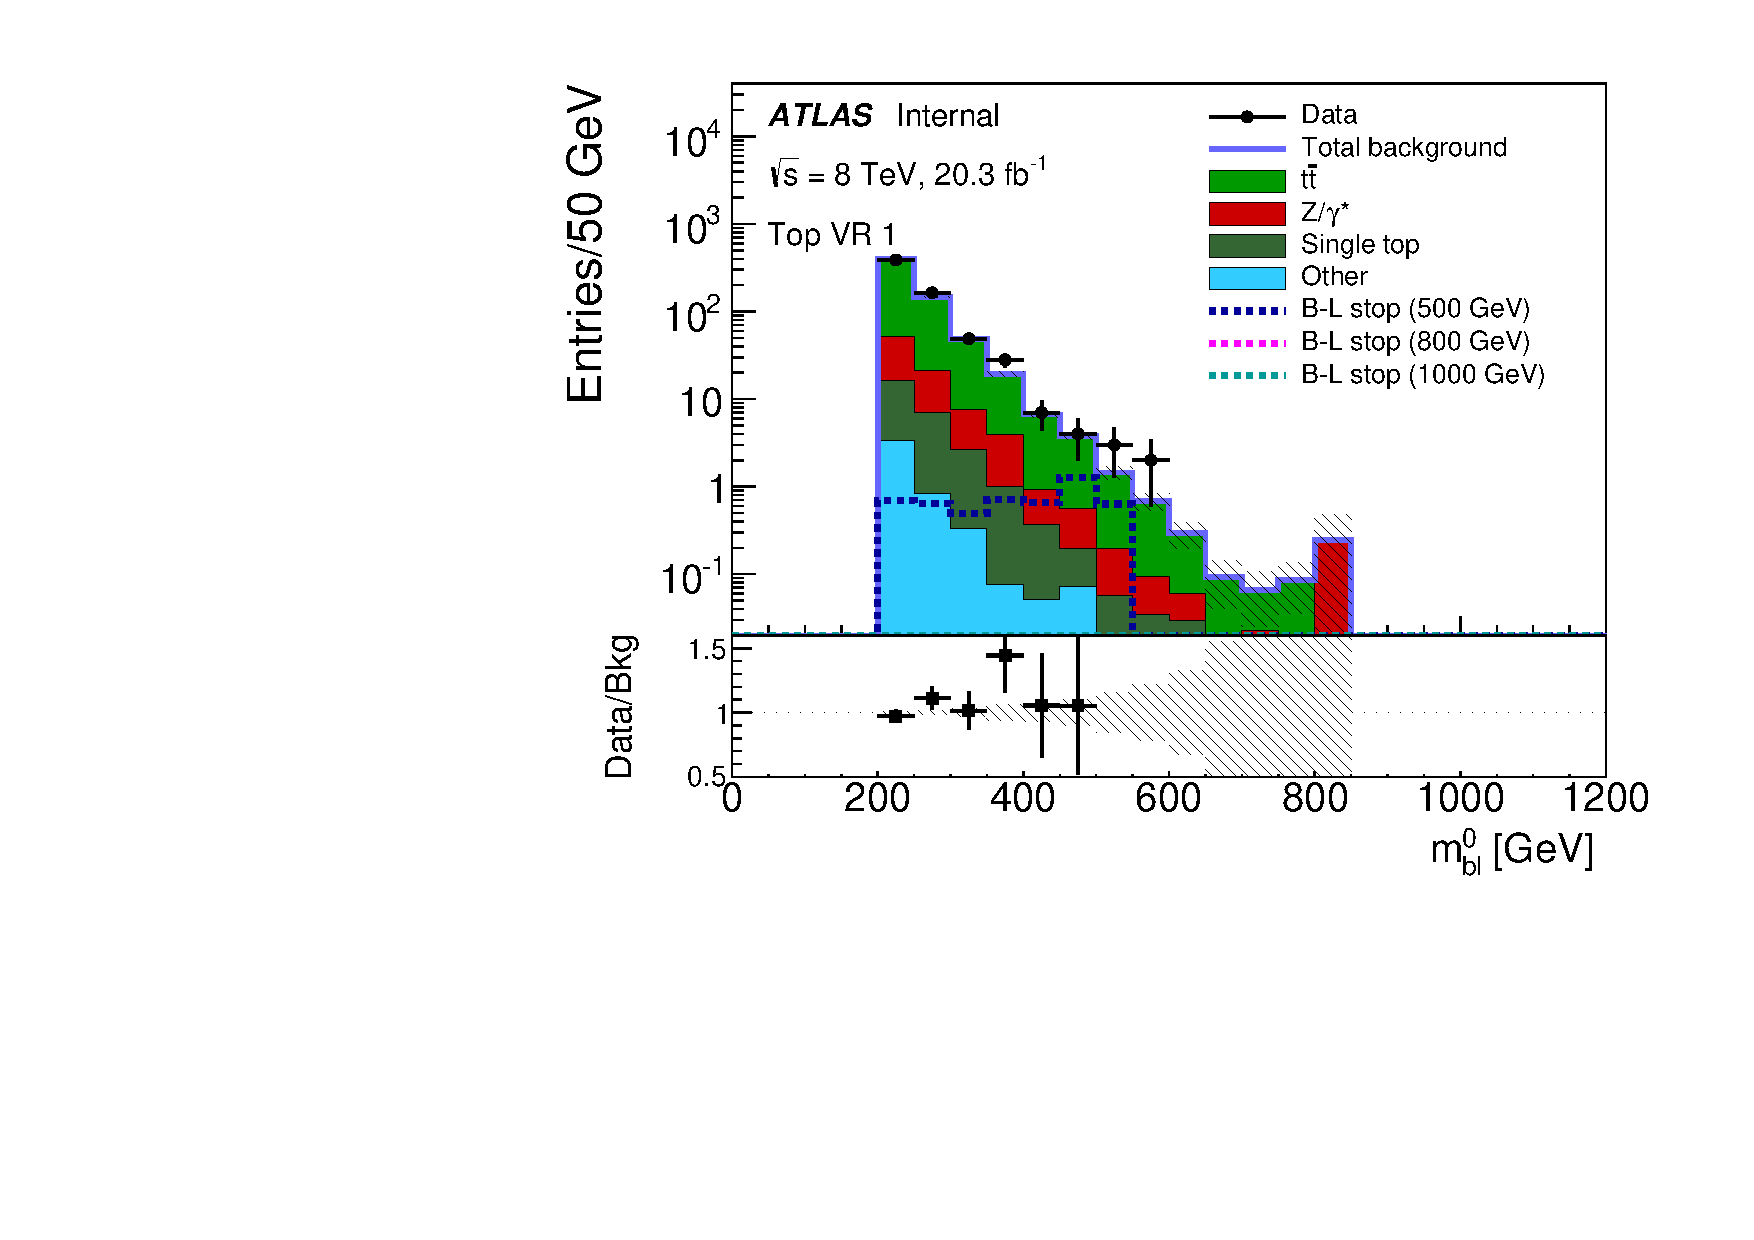
\includegraphics[width=0.48\textwidth, clip=true, trim=0 0 1cm 0]
      {figs/blstop/w_data__w_k_factor__dists/flavor_all__mbl_0__BMINUSL_VR_TOP_1_MBL_200__log.pdf}
  }
  \subbottom[Top VR 2]{
    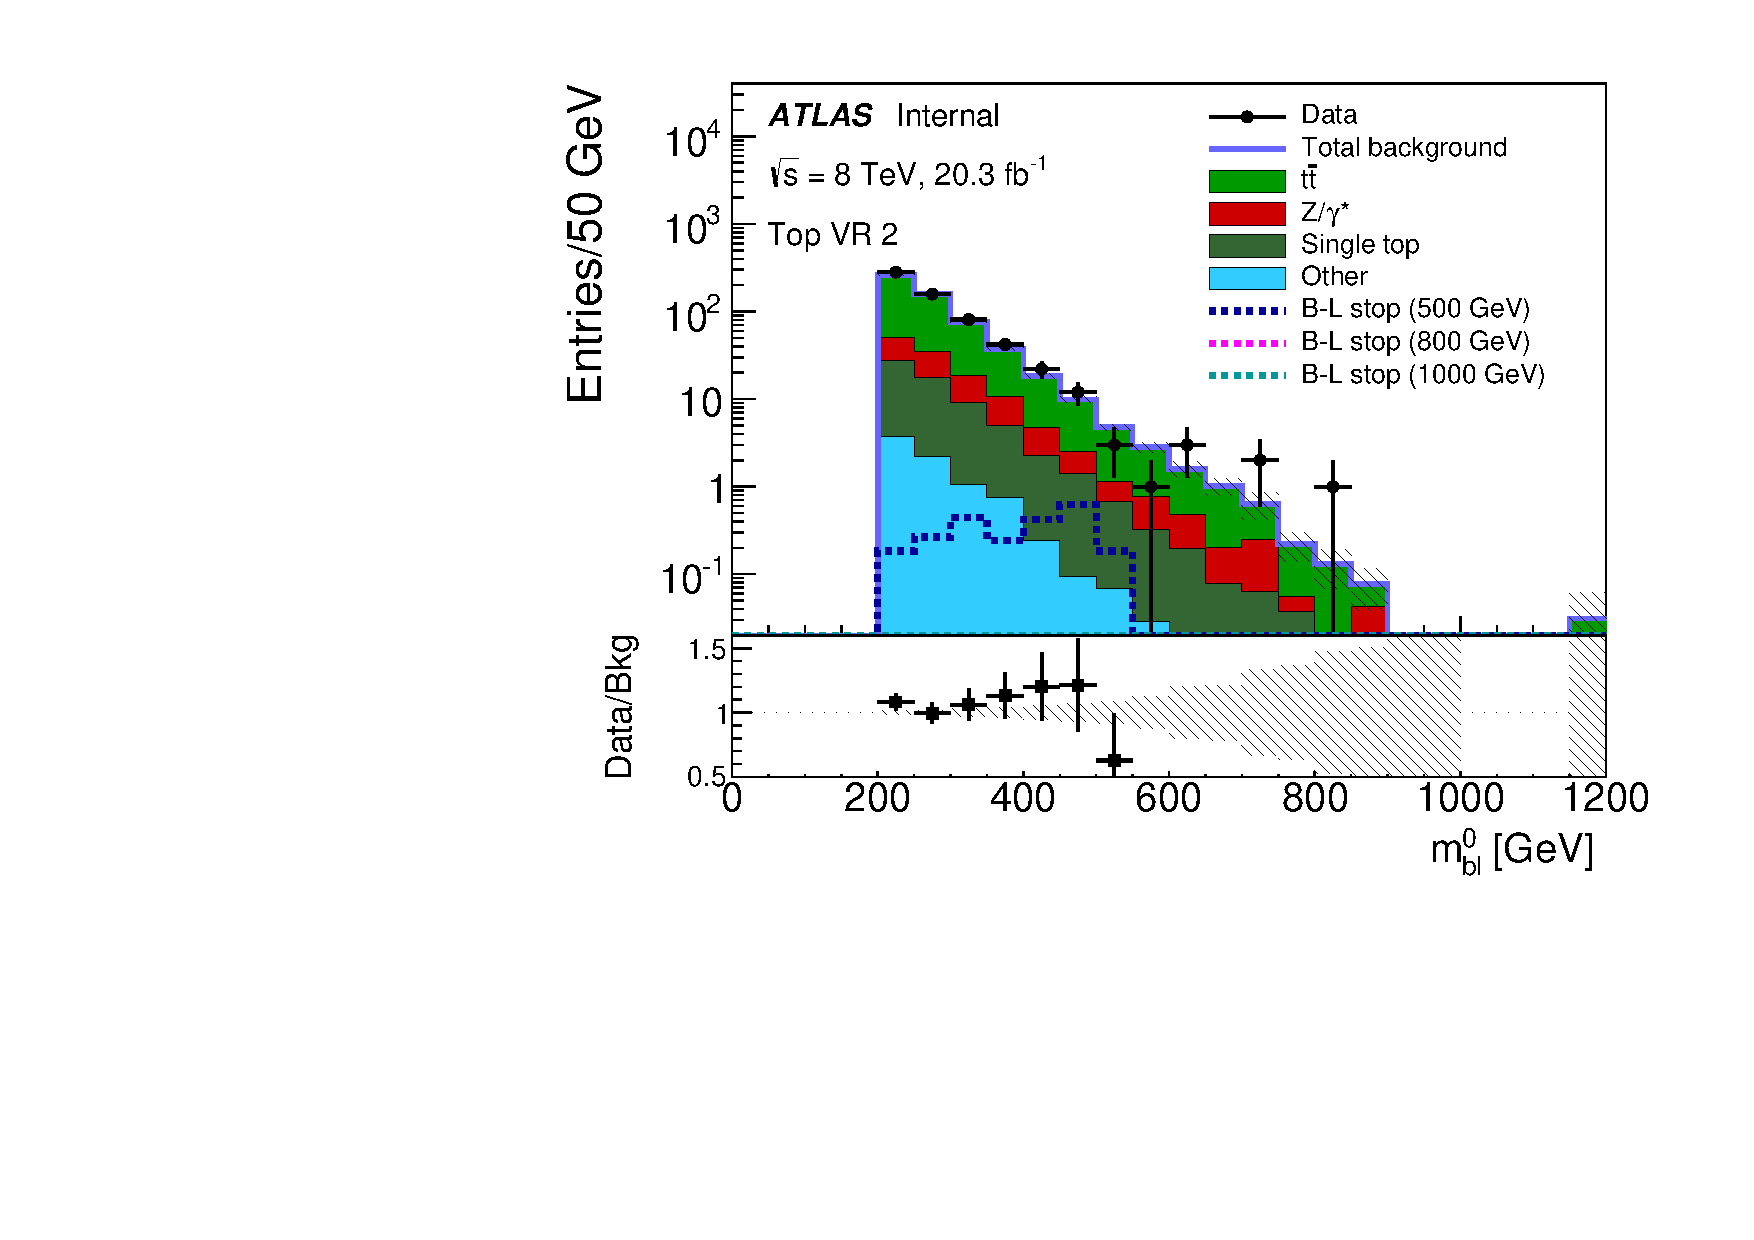
\includegraphics[width=0.48\textwidth, clip=true, trim=0 0 1cm 0]
      {figs/blstop/w_data__w_k_factor__dists/flavor_all__mbl_0__BMINUSL_VR_TOP_2_MBL_200__log.pdf}
  }
  \subbottom[Top VR 3]{
    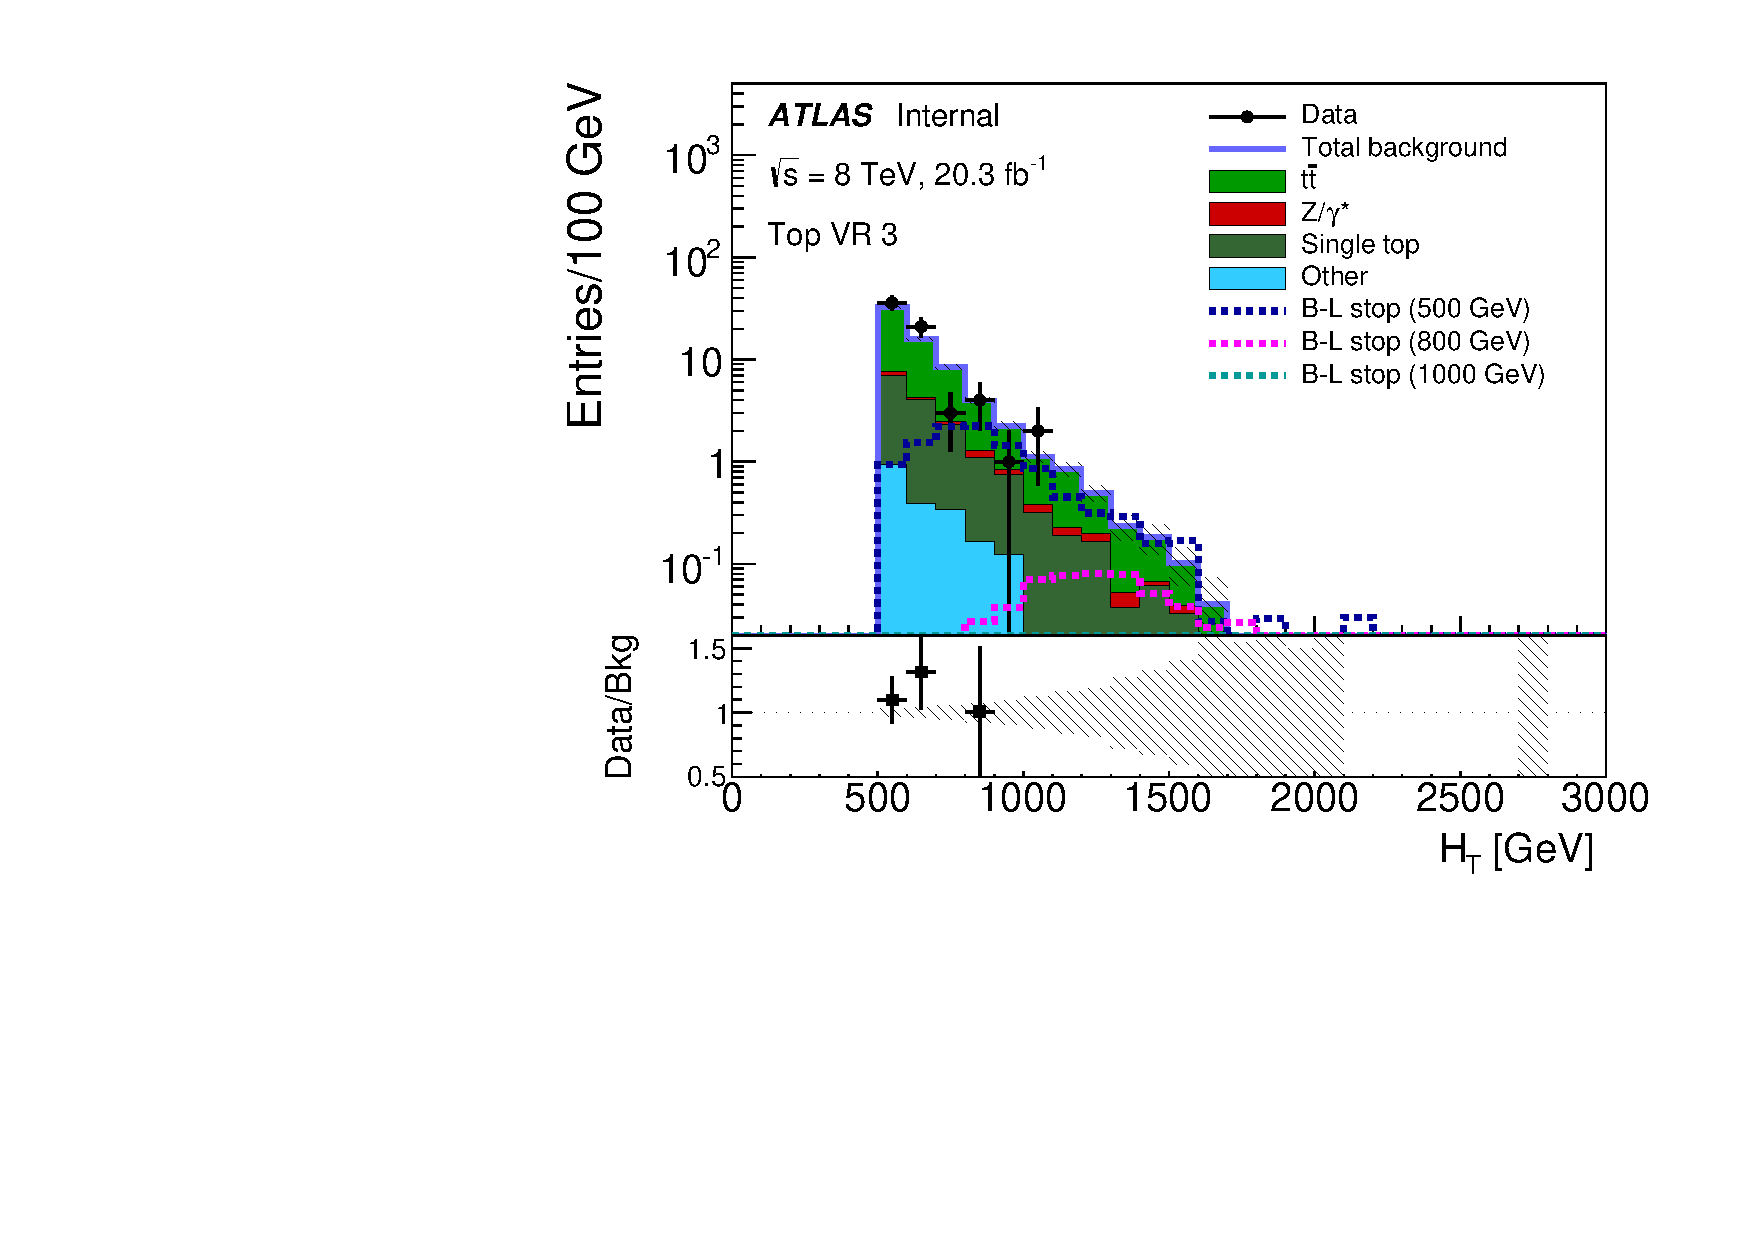
\includegraphics[width=0.48\textwidth, clip=true, trim=0 0 1cm 0]
      {figs/blstop/w_data__w_k_factor__dists/flavor_all__ht_signal__BMINUSL_VR_TOP_3_MBL_200__log.pdf}
  }
  \subbottom[$Z$ VR]{
    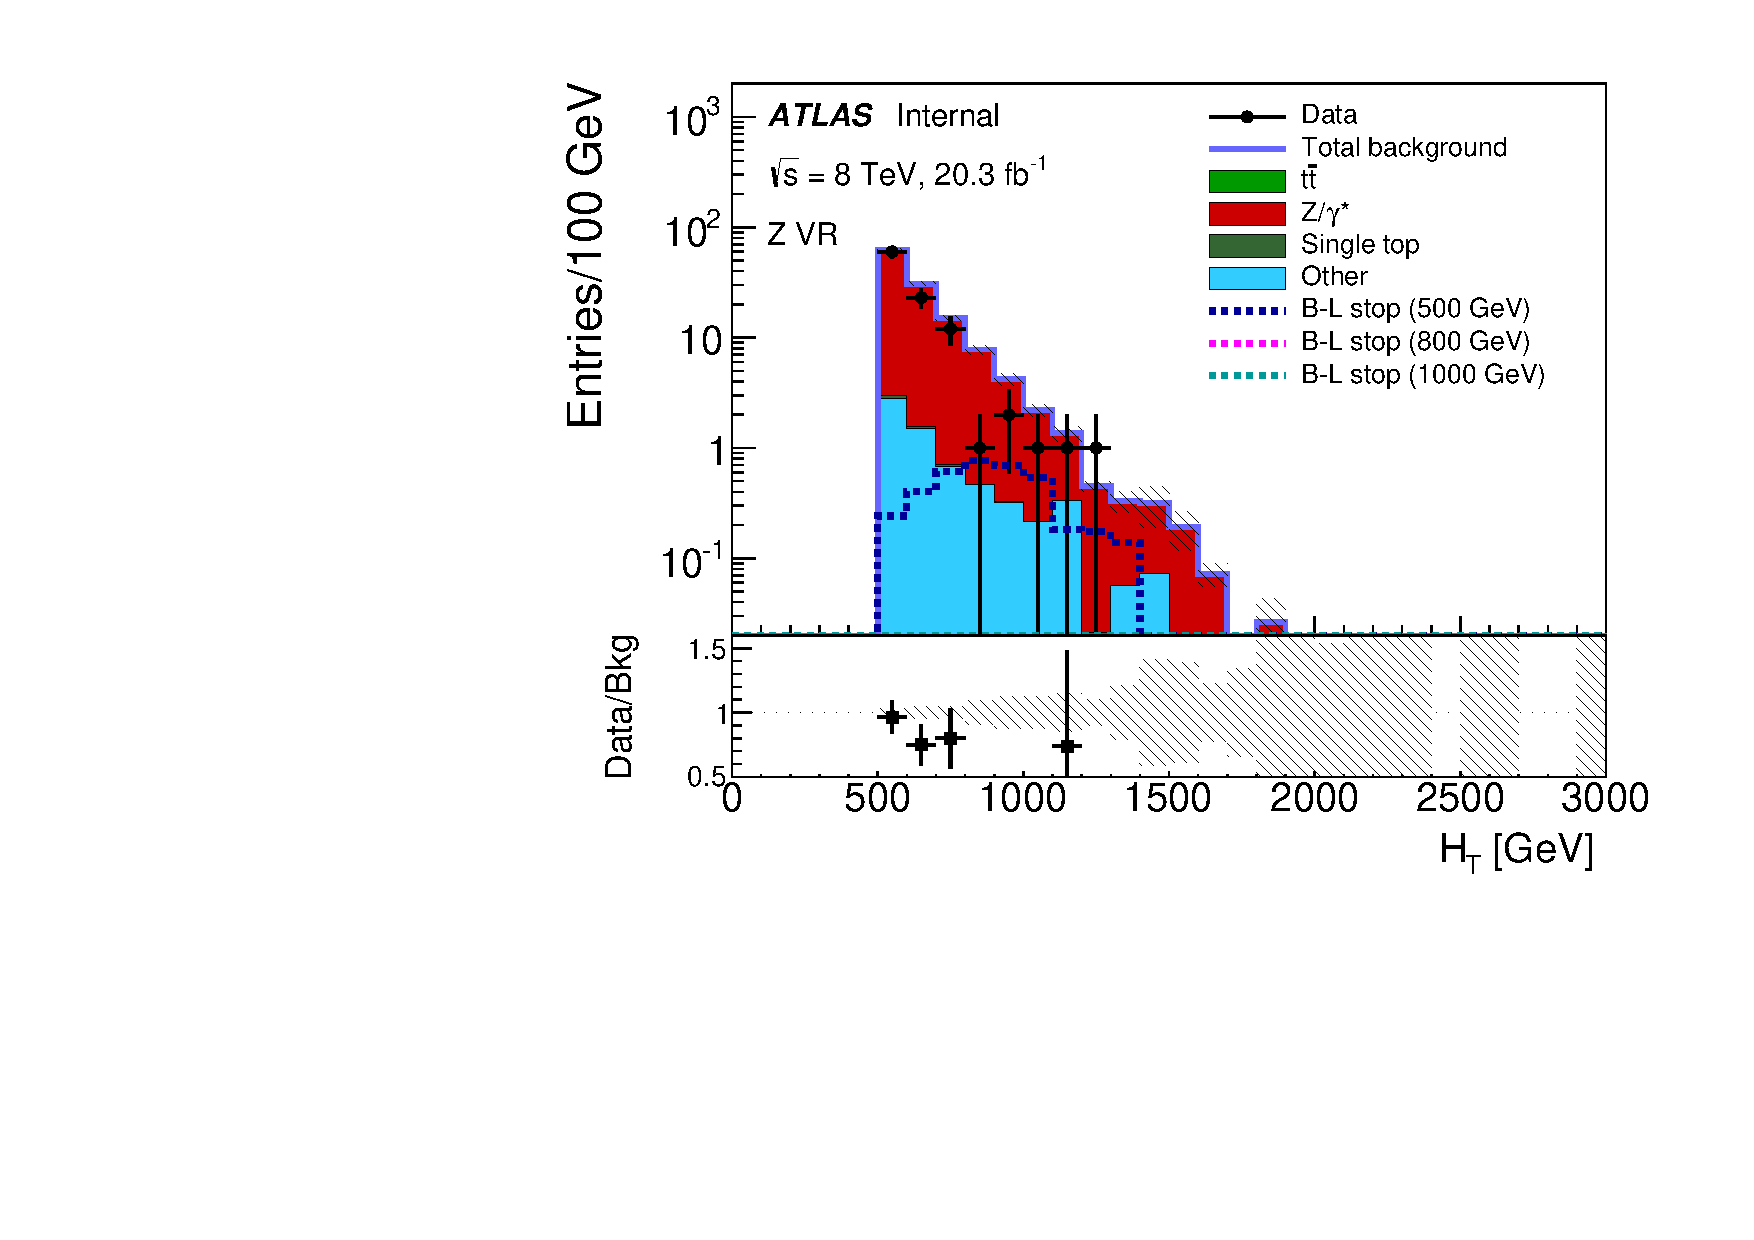
\includegraphics[width=0.48\textwidth, clip=true, trim=0 0 1cm 0]
      {figs/blstop/w_data__w_k_factor__dists/flavor_all__ht_signal__BMINUSL_VR_Z_MBL_200__log.pdf}
  }
  \caption{Expected and observed \MBL\ and \HT\ distributions in the
    VRs and the $Z$ VR after applying the $k_Z$ normalization factor derived
    in the $Z$ CR when all flavor channels are combined.
    % In each plot, the last bin includes the overflow for values beyond the
    % maximum shown.
    The hashed error bands show only the statistical uncertainty in the
    background MC simulation samples.
    The signal models have an assumed
    $Br(\tilde{t}\rightarrow be) = Br(\tilde{t}\rightarrow b\mu) = 0.5$.
    {\color{red} TODO remake with dashed line in ratio.}
  }
  \label{fig:vr_dists_w_norm_factor}
\end{figure}





%% -----------------------------------------------------------------------------
\FloatBarrier
\subsection{Background fit}
\label{sec:bkg_fit}

The normalization of the \TTBAR\ and the \ZGAMMAJETS\ backgrounds are
determined using a simultaneous fit, which takes into account
cross-contamination of the different background processes between the
CRs as well as the statistical and systematic uncertainties (described in
Section~\ref{sec:systematics}).
The fit is implemented using the \texttt{HistFitter} version~1.2.1, a framework
for statistical data analysis~\cite{Baak:2014wma}.
The remaining background estimates, due to  single top and other SM processes,
are taken from the MC simulation.

The background-only estimate is performed using a maximum likelihood fit
to the data in the Top and Z CRs.
The three flavor channels ($ee$, $\mu\mu$, and $e\mu$) are summed over, and the
total event yield in each CR is considered.
The predicted event yield for a background process $p$ (\TTBAR\ or \ZGAMMAJETS)
in a particular region $r$ is $\mu_{p} \cdot N_{r,p}^\mathrm{MC}$, where
$N_{r,p}^\mathrm{MC}$ is the number of events from process $p$ in region $r$
predicted by the MC simulation estimate, after applying all the relevant
scale factors and efficiencies.
$\mu_{p}$ is a strength parameter for each process which enters the likelihood
fit, and is used to model any under/over-prediction in the MC simulation
which is assumed to be constant across all regions.
A strength parameter is defined for the \TTBAR\ and \ZGAMMAJETS\ background
predictions, $\mu_{\TTBAR}$ and $\mu_\mathrm{Z}$ respectively.

The background fit is performed by first summing the total background estimate
for all background processes in each of the CRs.
The strength parameters are varied to obtain the best agreement between
the observed event yields and the background predictions.
The systematic uncertainties are treated as Gaussian nuisance parameters.
The background only fit finds that the best fit values for $\mu_{\TTBAR}$ and
$\mu_\mathrm{Z}$ are $1.11 \pm 0.14$ and $1.43 \pm 0.19$ respectively.
It should be noted that the $\mu_Z$ is consistent with the $k_Z$
derived in Section~\ref{sec:cr}.

The number of observed events as well as the post-fit expected number
of events in each of the CRs and VRs are shown in
Table~\ref{tab:bkg_only_fit_results}.
The agreement between the observed number of events and the fitted event
yields in the CRs and VRs is summarized in
Figures~\ref{fig:pull_dist_cr} and~\ref{fig:pull_dist_vr} respectively.
Using the fitted backgrounds, the dominant process in the same-flavor
channels of the SRs is \ZGAMMAJETS\ followed by single top and
\TTBAR. In the $e\mu$ channel, the \ZGAMMAJETS\ background does
not contribute, thus, the largest backgrounds are single top and \TTBAR.

As a result of the fit, the \ZGAMMAJETS\ background is scaled up by
approximately 40\%.
Due to this large normalization factor, the background is over-predicted in
the $Z$ VR.
The over-prediction is understood to be due to the difficulty in modeling
the production of \ZGAMMA\ in association with heavy flavor quarks.
This mismodeling is also observed by ATLAS in the SM measurement of
the $Z$~boson differential cross section~\cite{Aad:2013ysa,Aad:2014dvb}.
To account for this over-prediction, an additional systematic uncertainty of
50\% is taken on the background estimate from \ZGAMMAJETS\ events in regions
with large values of \HT.
This is described in Section~\ref{sec:systematics} along with the other
systematic uncertainties.

% - - - - - - - - - - - - - - - - - - - - - - - - - - - - - - - - - - - - - - -
\begin{table}[ht]
  \caption{The observed and expected event yields in the CRs and VRs. The
    expected event yields are shown before and after a fit to the data in
    the CRs. The fitted background yields in the CRs match the observed
    number of events in data by construction.
  }
  \label{tab:bkg_only_fit_results}
  %
  \begin{center}
    \begin{tabular}{lrrrrrr}
      \toprule
                         & Top CR           & Z CR            & Top VR 1       & Top VR 2      & Top VR 3        & Z VR            \\
      \midrule
      Observed           & $369$            & $327$           & $645$          & $606$         & $67$            & $101$           \\
      \midrule
      Fitted background  & $369   \pm 19$   & $327  \pm 18$   & $690  \pm 50$  & $630 \pm 40$  & $72   \pm 5$    & $130  \pm 60$   \\
      \midrule
      Fitted \TTBAR      & $346   \pm 19$   & $9.1  \pm 0.7$  & $600  \pm 40$  & $497 \pm 35$  & $54   \pm 5$    & $2.99 \pm 0.24$ \\
      Fitted \ZGAMMAJETS & $3.2   \pm 0.5$  & $309  \pm 18$   & $63   \pm 5$   & $64  \pm 5$   & $1.5  \pm 0.8$  & $120  \pm 60$   \\
      Single top         & $16.7  \pm 2.0$  & $0.83 \pm 0.09$ & $23.0 \pm 2.6$ & $56  \pm 6$   & $14.1 \pm 1.9$  & $0.32 \pm 0.04$ \\
      Other              & $2.83  \pm 0.27$ & $8.64 \pm 1.0$  & $4.7  \pm 0.4$ & $8.2 \pm 0.8$ & $2.03 \pm 0.27$ & $6.4  \pm 0.7$  \\
      \midrule
      Input SM           & $330$            & $230$           & $614$          & $557$         & $66$            & $93$            \\
      \midrule
      Input \TTBAR       & $310$            & $8.2$           & $543$          & $447$         & $49$            & $2.7$           \\
      Input \ZGAMMAJETS  & $2.2$            & $220$           & $44$           & $45$          & $1.1$           & $83$            \\
      Input single top   & $17$             & $0.8$           & $23$           & $57$          & $14$            & $0.30$          \\
      Input other        & $2.8$            & $8.6$           & $4.7$          & $8.2$         & $2.0$           & $6.40$          \\
      \bottomrule
    \end{tabular}
  \end{center}
\end{table}

\begin{figure}[ht]
\centering
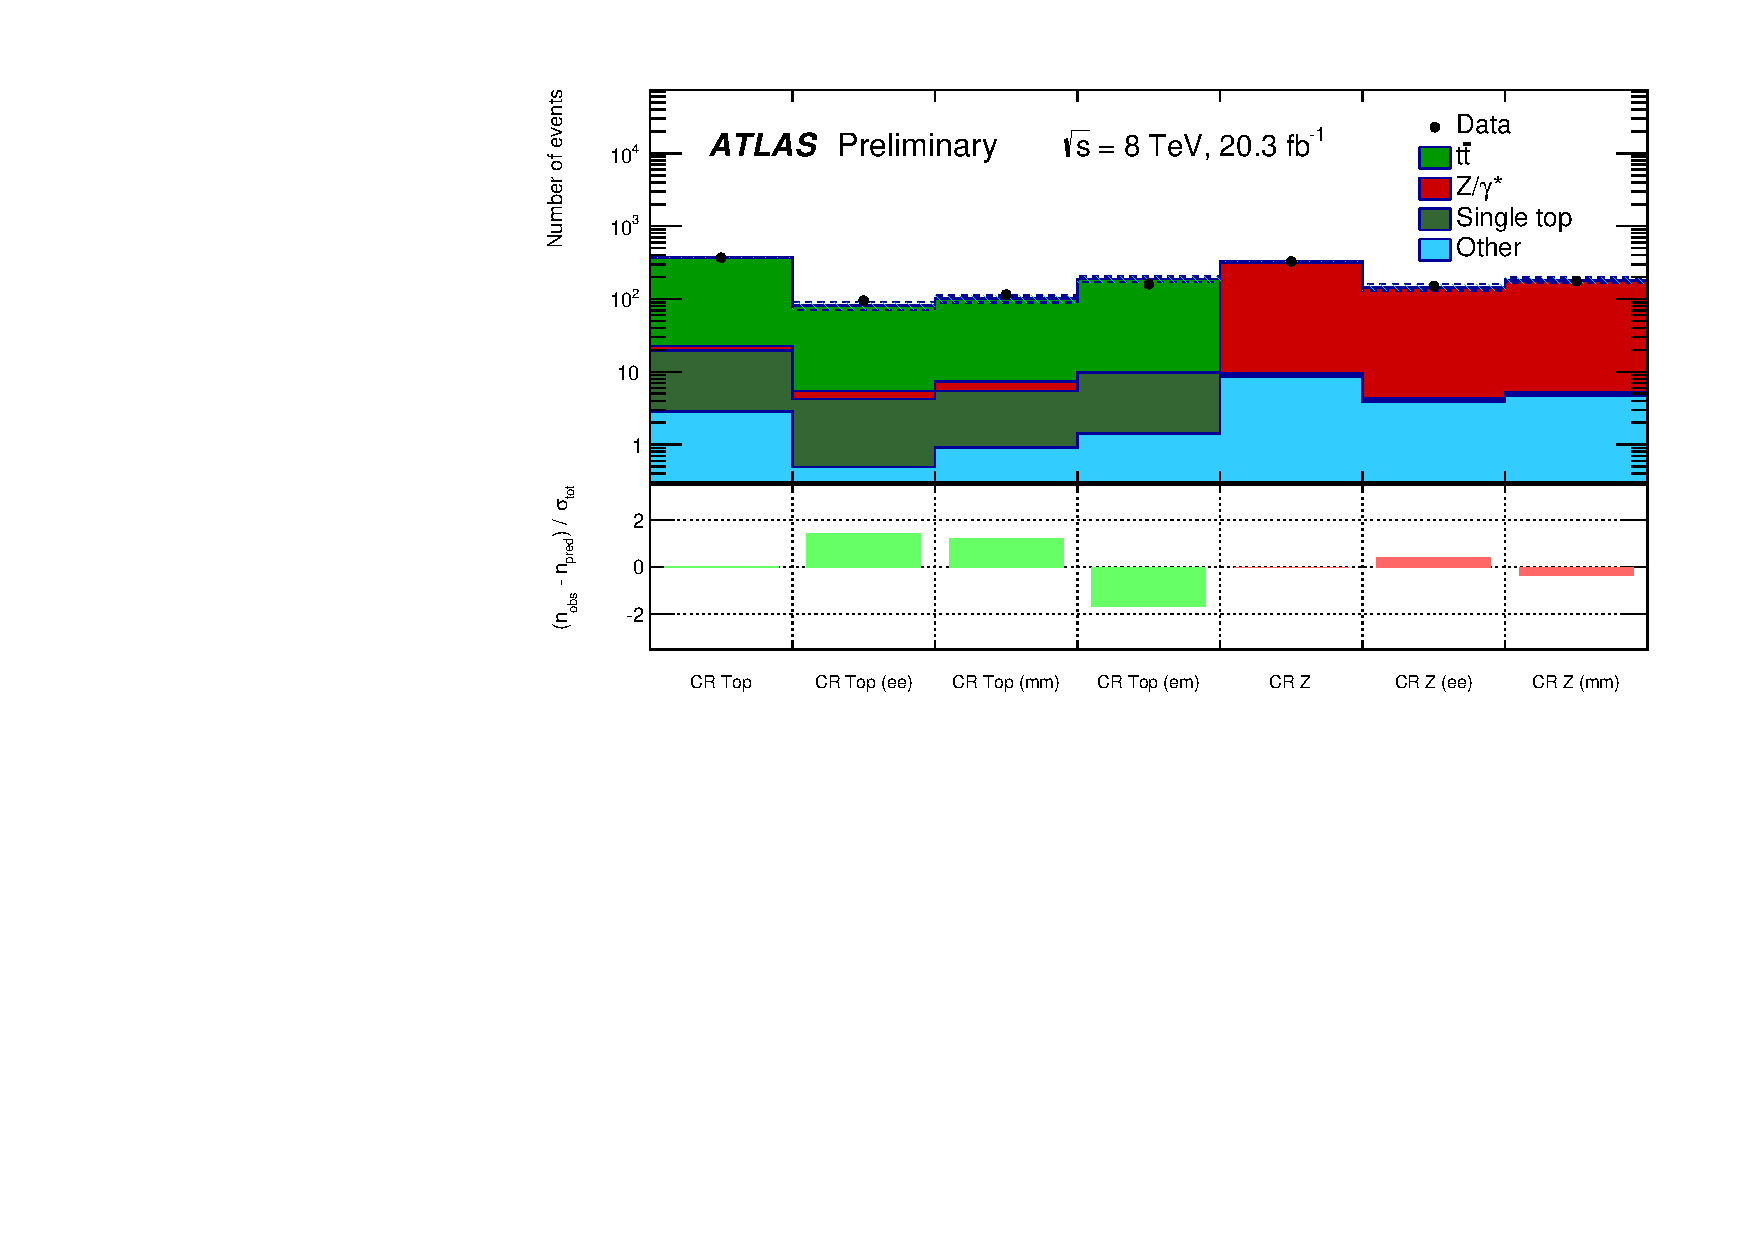
\includegraphics[width=\textwidth]{figs/blstop/histpull_CR_detailed.pdf}
\caption{The number of observed and expected events in the CRs,
  broken down by flavor channel and for each di-lepton flavor channel.
  The uncertainty band includes the statistical uncertainty as well as the
  systematic uncertainty (described in Section~\ref{sec:systematics}).
  The deviation of that channel's prediction from the observed number of events
  divided by the uncertainty in the prediction is also shown.
  The normalization of the background yields are determined
  by fitting the \TTBAR\ and \ZGAMMAJETS\ backgrounds to the observed
  data in the two CRs, so the Top CR and $Z$ CR bins have perfect agreement by
  construction.
}
\label{fig:pull_dist_cr}
\end{figure}

\begin{figure}[ht]
\centering
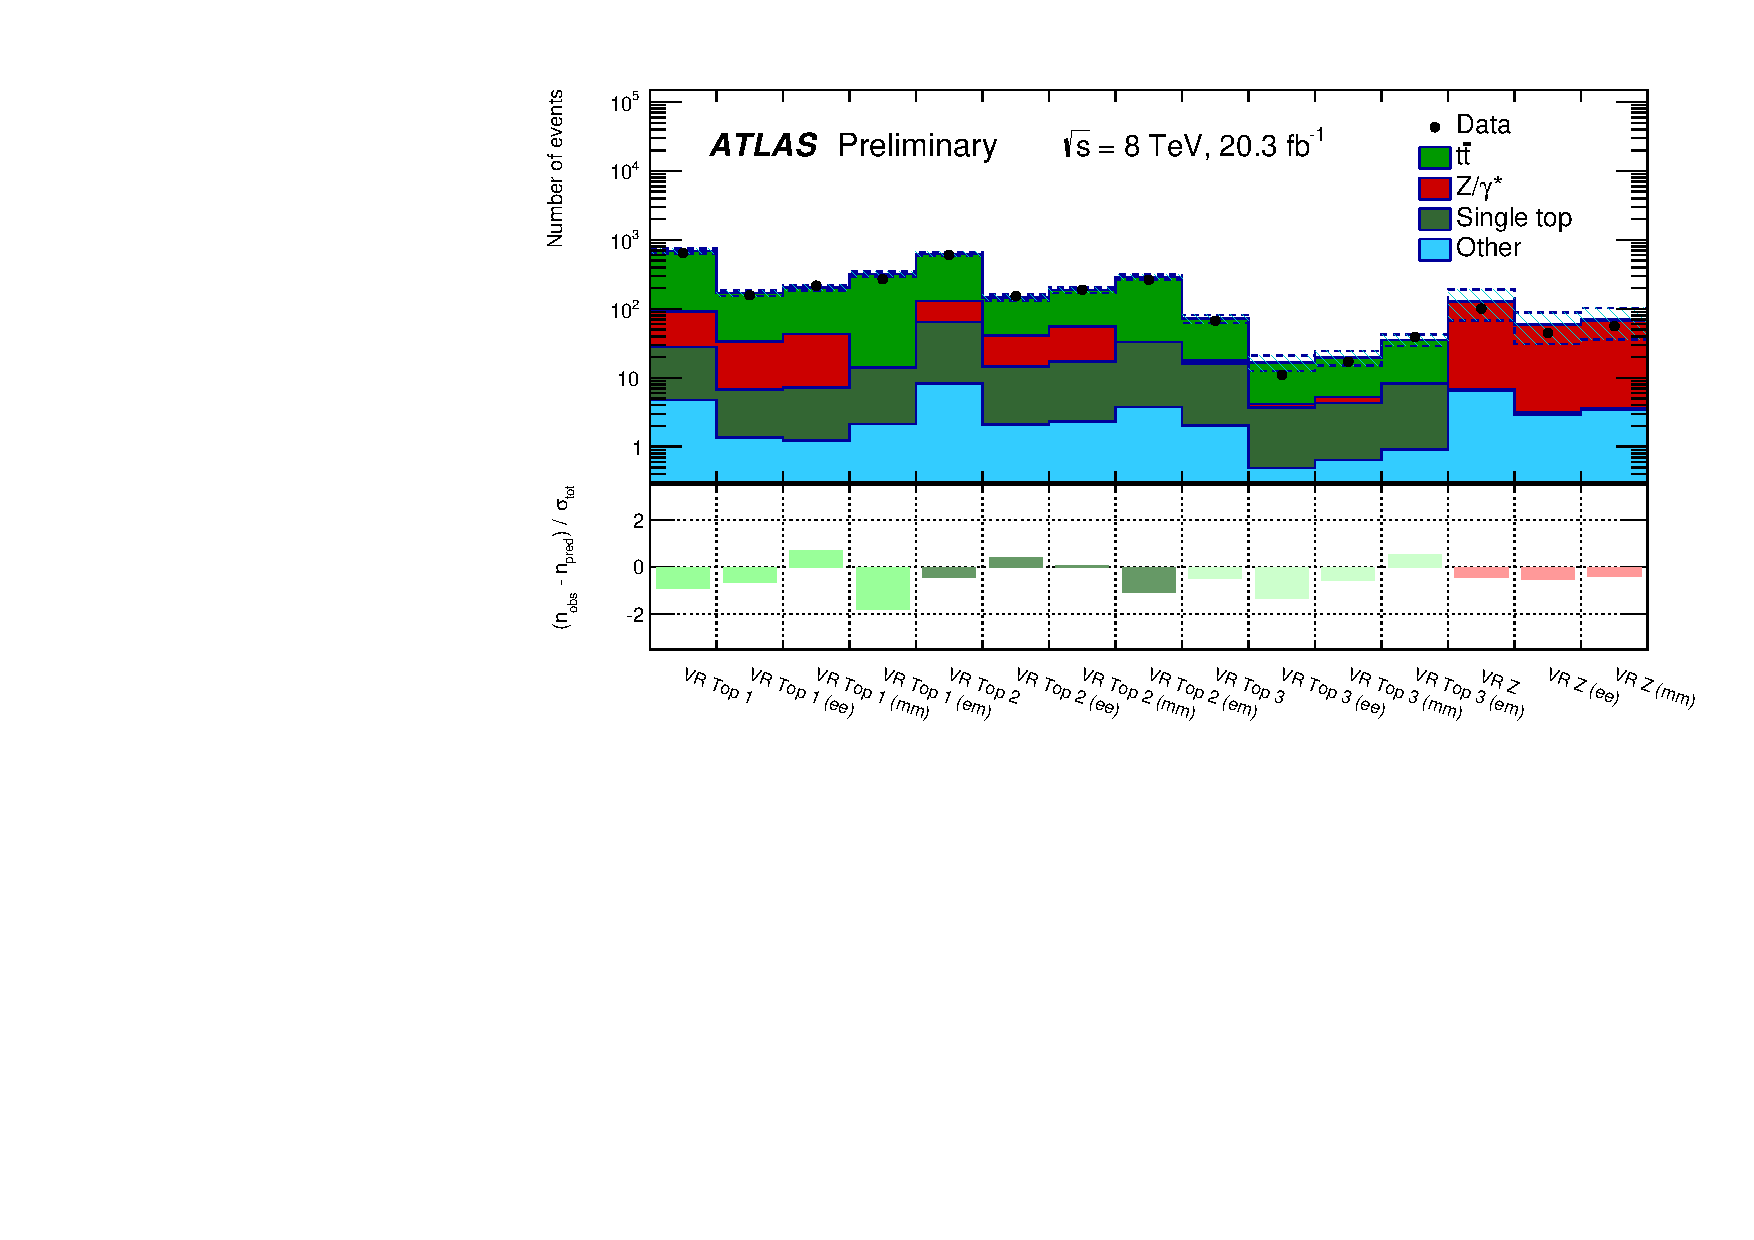
\includegraphics[width=\textwidth]{figs/blstop/histpull_VR_detailed.pdf}
\caption{The number of observed and expected events in the VRs,
  broken down by flavor channel and for each di-lepton flavor channel.
  The uncertainty band includes the statistical uncertainty as well as the
  systematic uncertainty (described in Section~\ref{sec:systematics}).
  The deviation of that channel's prediction from the observed number of events
  divided by the uncertainty in the prediction is also shown.
  The normalization of the background yields are determined
  by fitting the \TTBAR\ and \ZGAMMAJETS\ backgrounds to the observed
  data in the two CRs.
}
\label{fig:pull_dist_vr}
\end{figure}

The extrapolation from low \HT\ CRs to the high \HT\ region
where the SRs are located is validated using the Top VR 3
and $Z$ VR. These validation regions show fair
agreement between the observed and predicted event yields as well as
for the shape of the $\MBL^{0}$ and \HT\ distributions as shown in
Figures~\ref{fig:mbl_vr} and~\ref{fig:ht_vr}.

\begin{figure}
  \centering
  \subbottom[Top VR 3]{
    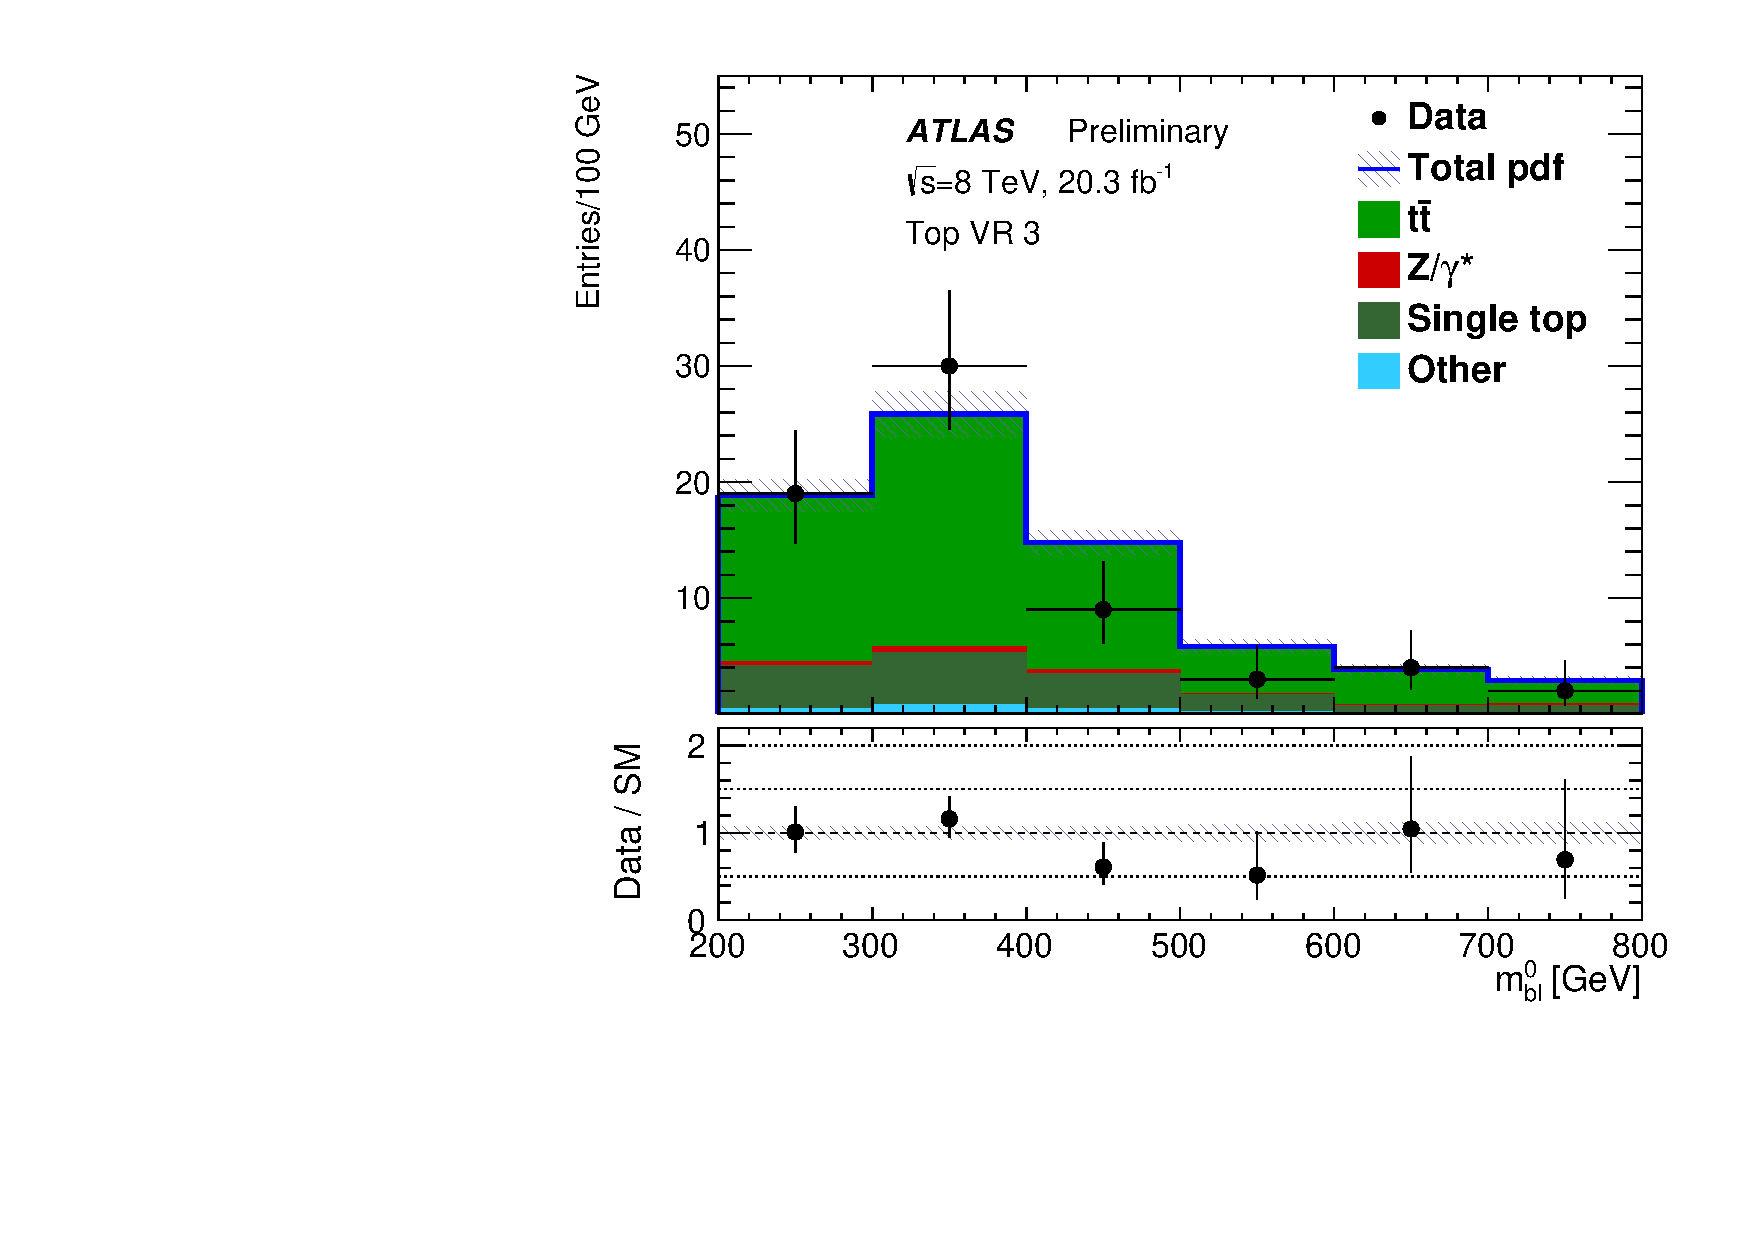
\includegraphics[width=0.48\textwidth]{figs/blstop/vr_top_3_mbl_0.pdf}
  }
  \subbottom[$Z$ VR]{
    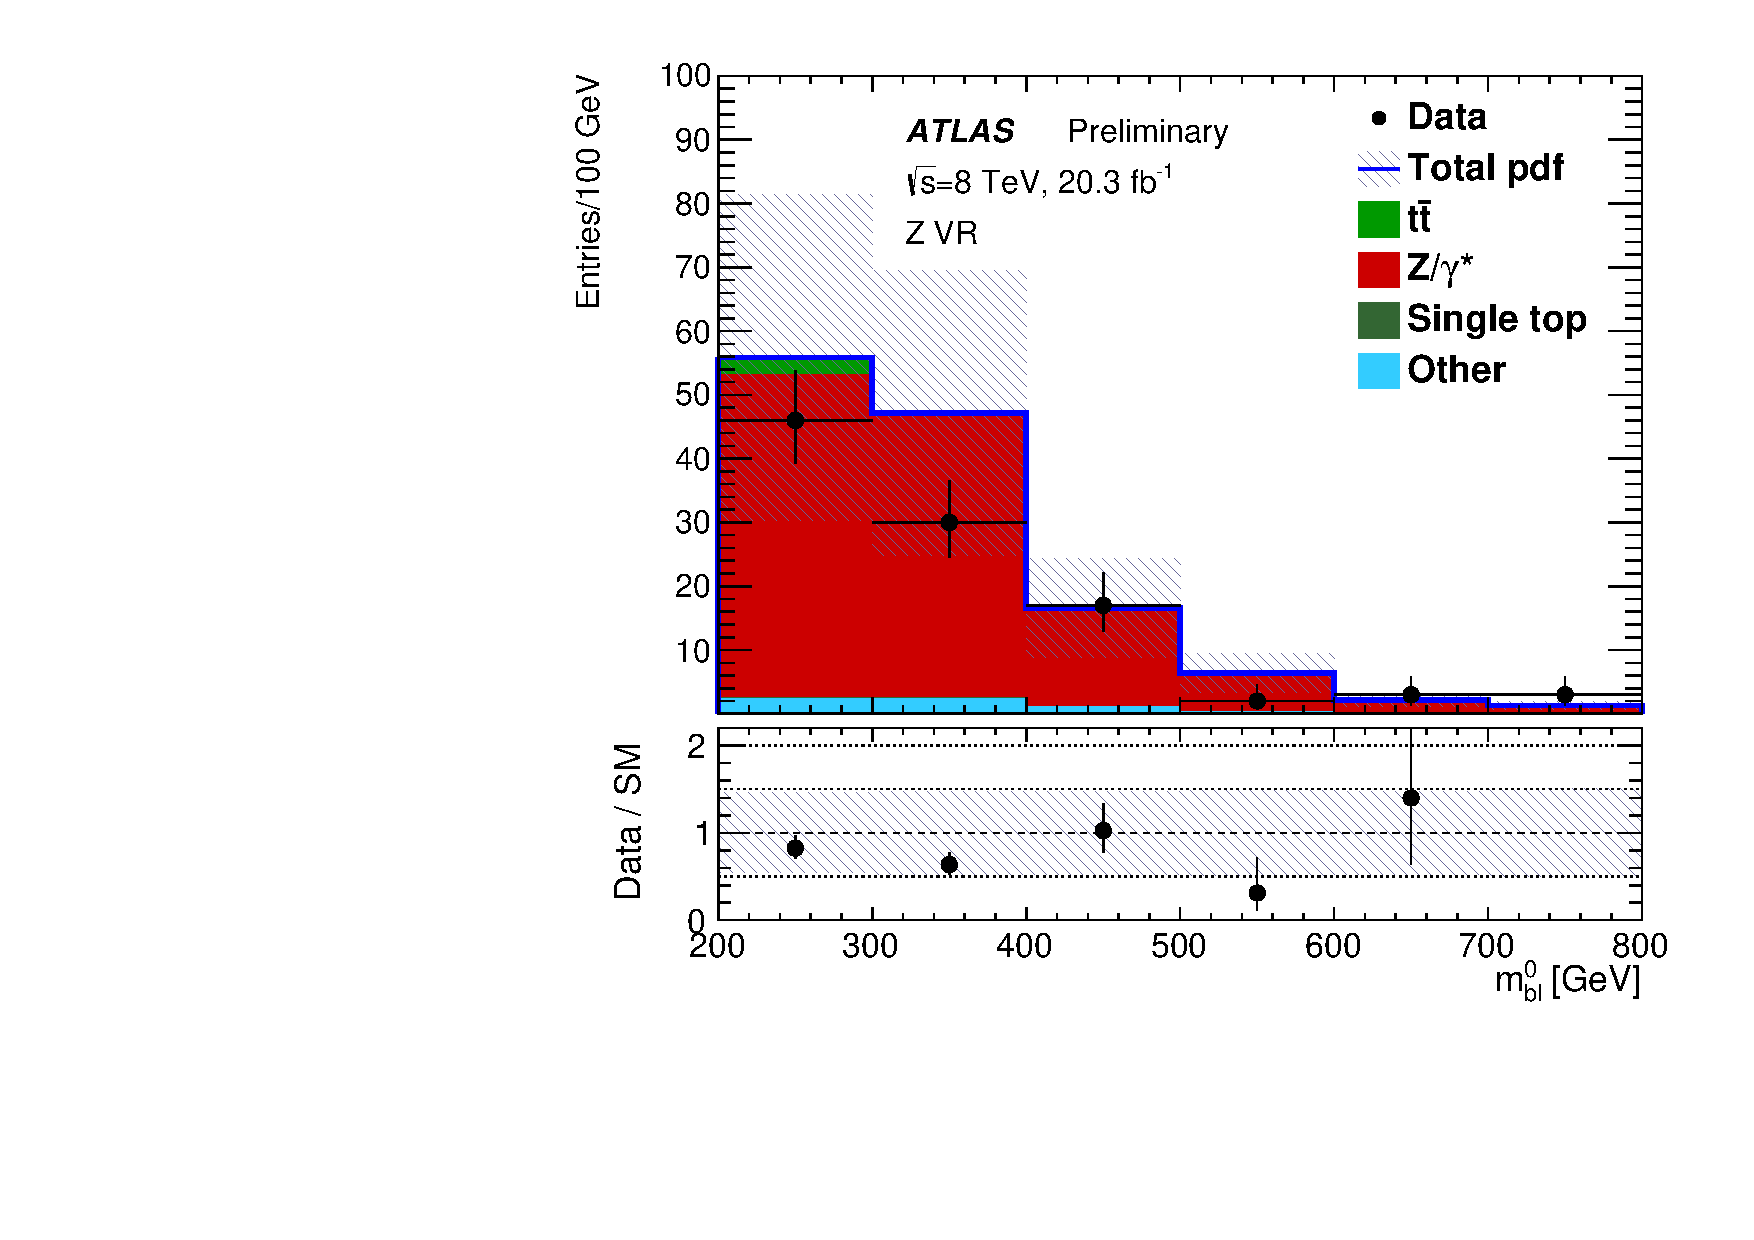
\includegraphics[width=0.48\textwidth]{figs/blstop/vr_Z_mbl_0.pdf}
  }
  \caption{The $\MBL^0$ distribution in Top VR 3 (left) and $Z$ VR (right).
    The Standard Model background prediction is shown after setting the
    normalization of the \TTBAR\ and \ZGAMMAJETS\ backgrounds based on the
    observed data in the CRs. The hashed bands show the uncertainty in the
    fitted background prediction including all statistical and systematics
    uncertainties.
    The bottom of each plot shows the ratio of the observed data to the
    Standard Model background prediction.
  }
  \label{fig:mbl_vr}
\end{figure}

\begin{figure}
  \centering
  \subbottom[Top VR 3]{
    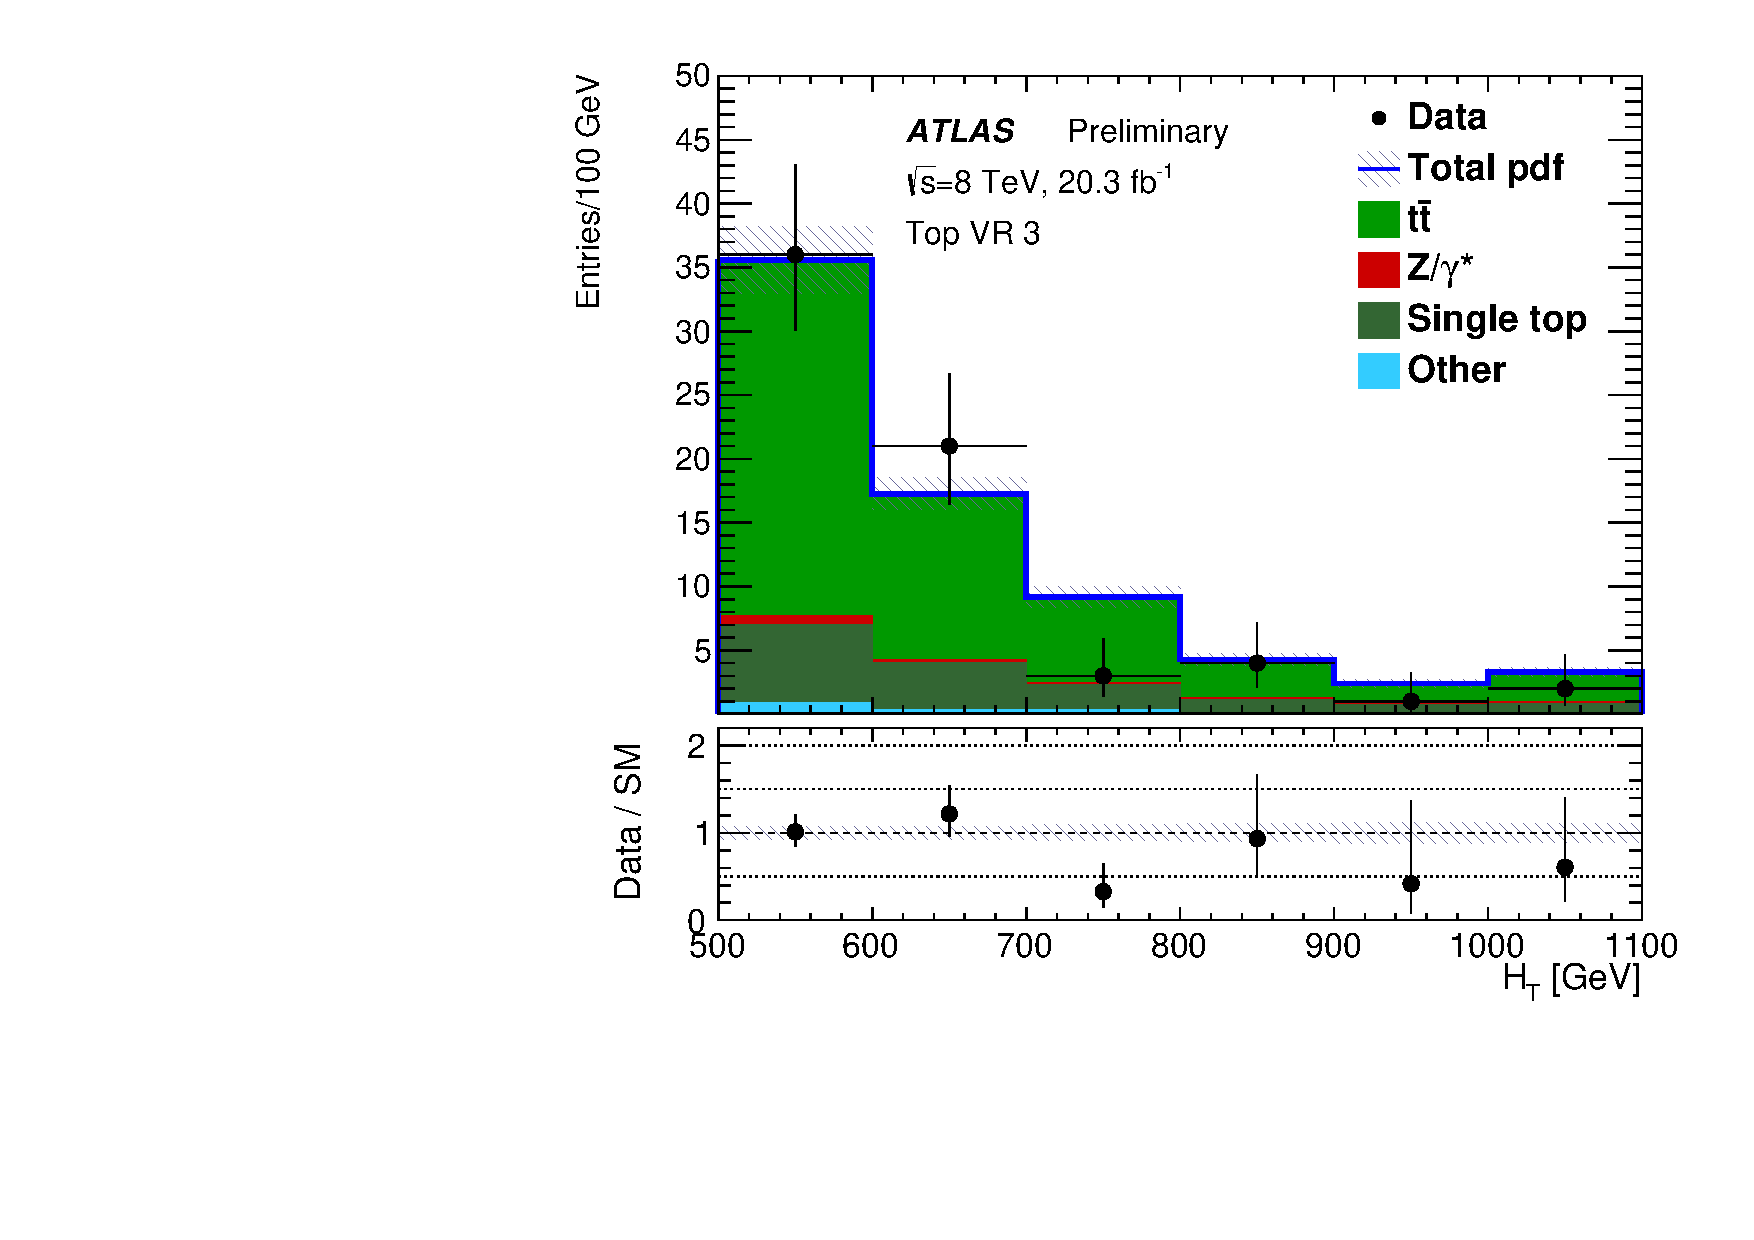
\includegraphics[width=0.48\textwidth]{figs/blstop/vr_top_3_ht_signal.pdf}
  }
  \subbottom[$Z$ VR]{
    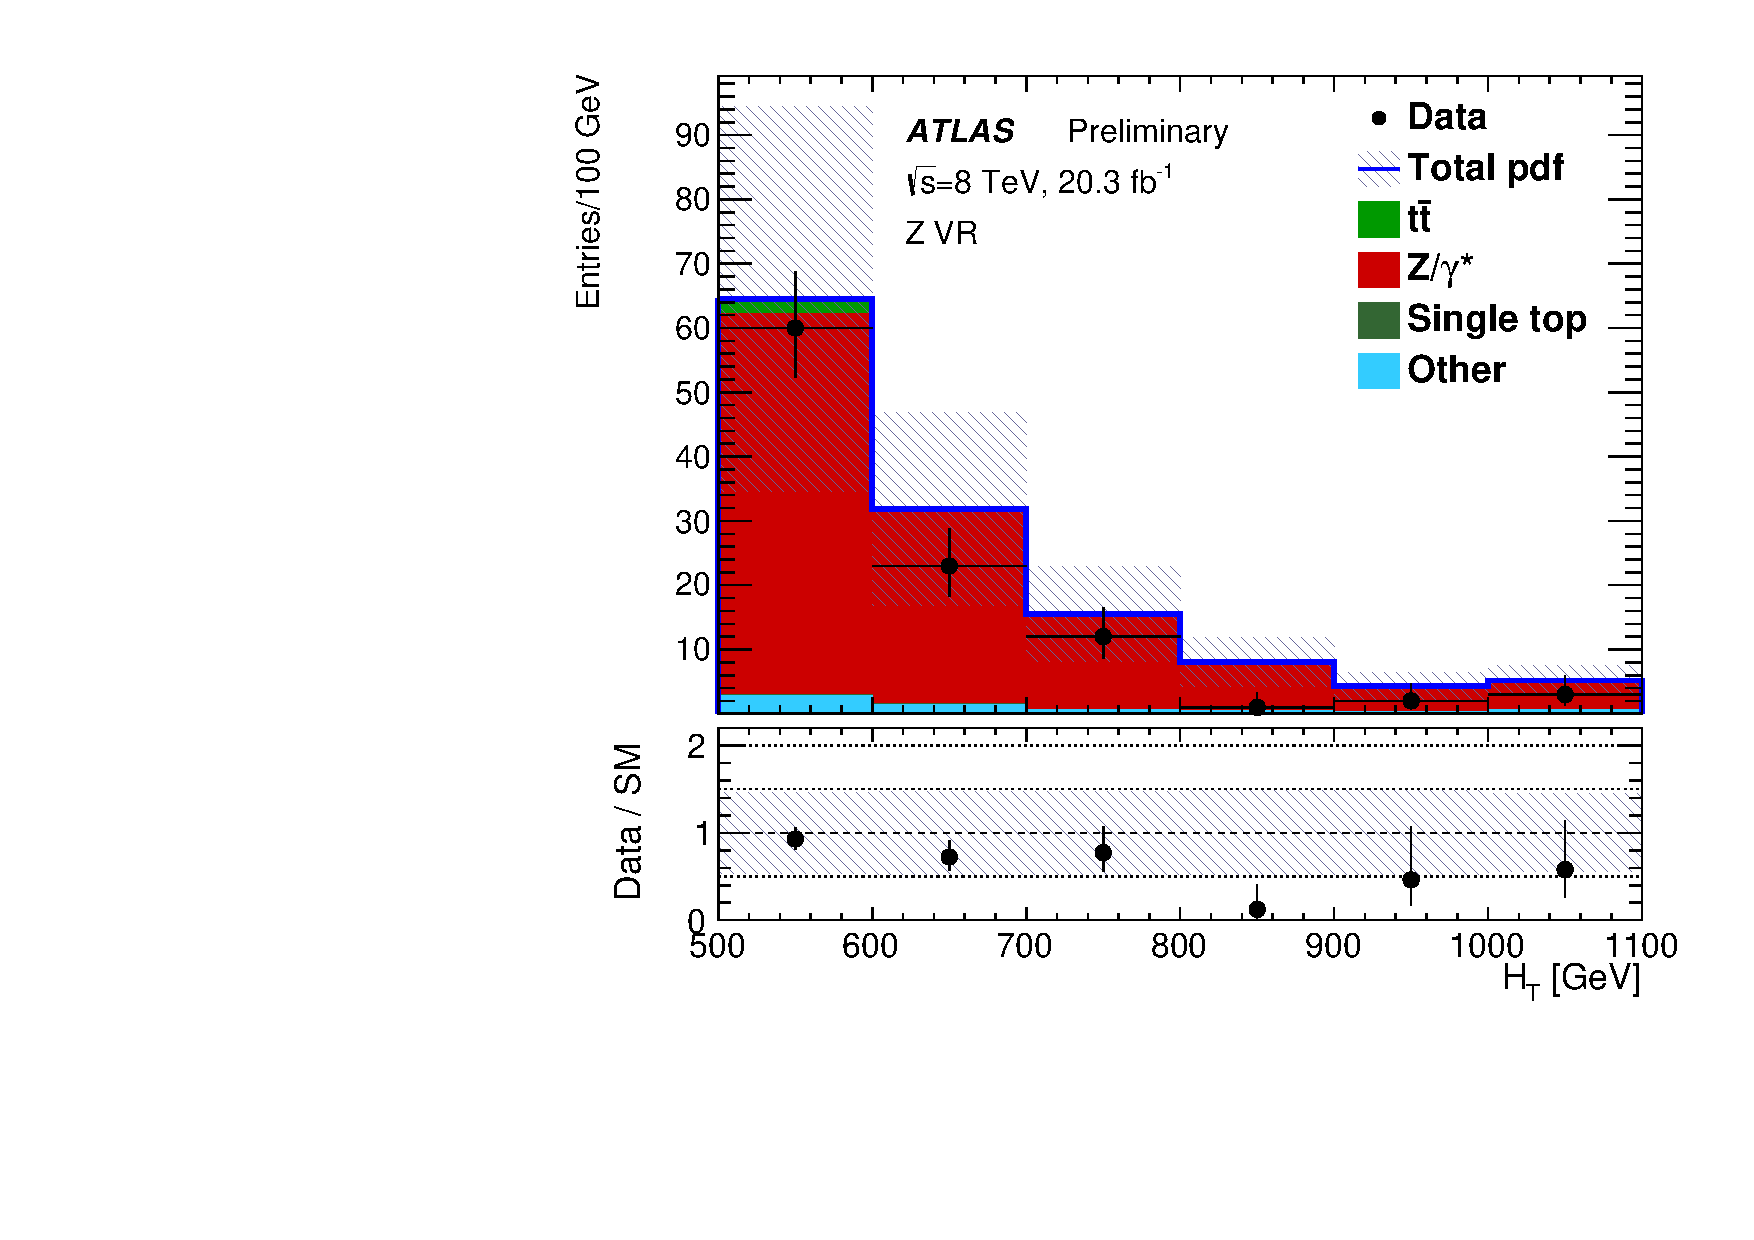
\includegraphics[width=0.48\textwidth]{figs/blstop/vr_Z_ht_signal.pdf}
  }
  \caption{The \HT\ distribution in Top VR 3 (left) and $Z$ VR (right).
    The Standard Model background prediction is shown after setting the
    normalization of the \TTBAR\ and \ZGAMMAJETS\ backgrounds based on the
    observed data in the CRs.
    The hashed bands show the uncertainty in the fitted background prediction
    including all statistical and systematics uncertainties.
    The bottom of each plot shows the ratio of the observed data to the
    Standard Model background prediction.
  }
  \label{fig:ht_vr}
\end{figure}


%% -----------------------------------------------------------------------------
\FloatBarrier
\section{Systematic uncertainties}
\label{sec:systematics}

Several sources of systematic
uncertainty are considered when determining the estimated signal and background
contributions.
The largest sources of systematic uncertainty are those related to the
MC statistical uncertainty in the SRs, the jet energy scale (JES), and
the $b$-tagging efficiency.
The uncertainty in the lepton energy scale and resolution was considered,
but shown to be negligible.

%% - - - - - - - - - - - - - - - - - - - - - - - - - - - - - - - - - - - - - - -
The uncertainty in the JES has an impact on both the jet
selection criteria and the derived kinematic variables of the event, such as
the \HT\ and the \MET\ measurements.
The JES uncertainty is evaluated using the EM+JES scheme as described
in~\cite{JES}, and the scaling is provided by the
\texttt{MultijetJESUncertaintyProvider} tool.
The uncertainty in the JES is composed of 16 parameters, and takes into account
the dependence on \pt, $\eta$, jet flavor, and the number of primary vertices.
The effect of each component on the event yield is estimated by varying the
component by $\pm 1 \sigma$ in the MC simulation and re-running the full event
selection, propagating the variation in the JES to the jet selection and related
kinematic quantities.

%% - - - - - - - - - - - - - - - - - - - - - - - - - - - - - - - - - - - - - - -
The uncertainty in the jet energy resolution (JER) is evaluated by applying an
additional smearing to the \pt\ measurement of each of the jets in the MC
simulation.
The size of the smearing is determined in dijet events as described
in~\cite{JER}.
The smearing is provided by the \texttt{JetSmearingTool} tool, and depends on
the \pt\ and \eta\ of the jets within an event.
The JER smearing alters the \pt\ of the jets within the event, and therefore
the event selection.
As with the JES, the JER uncertainty is evaluated by applying the smearing,
propagating the variations to the event kinematic variables, and
re-running the full event selection on MC simulation to determine the new
event yields.

%% - - - - - - - - - - - - - - - - - - - - - - - - - - - - - - - - - - - - - - -
The efficiency of the $b$-tagging
algorithms affects the overall yields in each of the analysis regions.
This includes the possibility of a light flavor jet being incorrectly tagged
as a $b$-jet, or a jet which initiated by a $b$-quark failing the $b$-tagging
requirement.
The $b$-tagging efficiency uncertainty is broken into three components,
corresponding to the tagging efficiency of $b$-jets, $c$-jets, and light
flavor jets (light quarks and gluons).
These uncertainties take into account the dependence on \pt\ and jet flavor.
For the MC simulation, the weight associated with the $b$-tagging scale factor
is varied up or down based on the specific parameter of interest, and used to
determine the uncertainty in the event yield.

%% - - - - - - - - - - - - - - - - - - - - - - - - - - - - - - - - - - - - - - -
The backgrounds are constrained in the CRs which are regions with low \HT,
while the SRs require high \HT.
Top VR 3 and $Z$ VR are used to assess any uncertainty associated with the
extrapolation from low \HT\ to high \HT.
The \TTBAR\ background extrapolation is assessed using Top VR 3. It can be seen
from Table \ref{tab:bkg_only_fit_results} that the post-fit background estimate
in Top VR 3 is in reasonably agreement with the observed data, so no additional
uncertainty is applied to the \TTBAR\ backgrounds due to the \HT\ extrapolation.
The \ZGAMMAJETS\ background extrapolation is assessed using the $Z$ VR.
The overall background is overpredicted in this region by 29\%, and the
prediction is the worst in the highest \HT\ bins.
An additional uncertainty of 50\% is applied to the \ZGAMMAJETS\ background
for events with $\HT > 500 \GeV$.
% An \HT\ extrapolation uncertainty of 50\% is applied to \ZGAMMAJETS\ events
% with $\HT \geq 500$~\GeV. This is assigned to account for uncertainty in
% the \ZGAMMAJETS\ \HT\ spectrum. This uncertainty is derived from the
% disagreement observed in Figures~\ref{fig:pull_dist_vr}-\ref{fig:ht_vr}.
%%

%% - - - - - - - - - - - - - - - - - - - - - - - - - - - - - - - - - - - - - - -
Several uncertainties related to the theoretical modeling of the major
background processes in MC simulation are considered.
These include the uncertainty in the cross sections, renormalization and
factorization scale variations, and generator uncertainties.
These uncertainties are evaluated by performing the event selection using only
the MC truth information, and comparing the expected event yields obtained
from MC simulation samples produced using different generator configurations.
An additional systematic uncertainty, due to the $\pm 2.8$\% uncertainty in the
integrated luminosity is evaluated for all background processes except
\TTBAR\ and \ZGAMMAJETS, because these backgrounds take the normalization from
data control regions.
A summary of the estimated effect of each source of systematic uncertainty
(both experimental and theoretical) is in Table~\ref{tab:systematic_breakdown}.

%% - - - - - - - - - - - - - - - - - - - - - - - - - - - - - - - - - - - - - - -
%% ttbar theory systematics
The sources of systematic uncertainty evaluated for the \TTBAR\ background
include the renormalization and factorization scale variations, MC generator
uncertainties, parton shower, and the amount of initial or final state
radiation (ISR or FSR) in the event.
%%
% scale variations
The scale variations are evaluated by comparing the expected event yields at the
truth level obtained using dedicated \TTBAR\ samples, each generated using
\powheg\ and \pythia, where the factorization and renormalization
scales are separately varied up and down by a factor of 2.
This isolates the effect of each of the scale variations.
% The difference in
% expected number of events in each region is taken to be the uncertainty in the
% \TTBAR\ background.
The differences in the expected event yields for these samples is take to be
the uncertainty due to the scale variations.
%%
% MC generator
The MC generator uncertainty accounts for the difference in the MC predictions
obtained using different generator programs.
These are assessed by comparing the truth level event selection for a
\TTBAR\ sample generated using \powheg\ and \jimmy\ with a sample
generated using \mcnlo\ and \jimmy.
Since \jimmy\ is used to perform the parton shower in both of these
samples, the differences can be attributed to the differences in the
generation rather than the parton shower step.

%%
% parton shower
The uncertainty in the parton shower in \TTBAR\ samples is estimated by
comparing the expected event yields using the truth level information for two
\TTBAR\ samples each generated using \powheg.
One sample uses \pythia\ for the parton shower step, while the other
uses \jimmy.
This isolates the parton shower part of the MC simulation, which is performed
either using \pythia\ or \jimmy.
%%
% ISR/FSR
The uncertainty in the ISR and FSR is evaluated by comparing the expected number
of events in a truth level event selection found in two \TTBAR\ samples, each
generated using \acermc\ and \pythia.
The two samples differ in the amount of ISR and FSR is included in the
simulation.
%%

%% - - - - - - - - - - - - - - - - - - - - - - - - - - - - - - - - - - - - - - -
%% single top theory systematics
For the single top background, the sources of systematic uncertainty
include the single top cross section, the MC generator uncertainties, the parton
shower, ISR and FSR, and the interference with \TTBAR.
%%
% cross section
Single top can be produced through three production channels, with production
cross sections
\begin{itemize}
  \item $s$-channel: $5.61 \pm 0.22$ pb
  \item $t$-channel: $87.76^{+3.44}_{-1.91}$ pb
  \item $Wt$-channel: $22.37 \pm 1.52$ pb.
\end{itemize}
It was shown that the $Wt$-channel is the dominant single top production
channel for the regions of interest.
For this reason, the 7\% uncertainty in the $Wt$-channel cross section is the
only single top cross section uncertainty which is considered.
%%
% MC gen uncertainty.
The MC generator uncertainty in the single top background estimate is evaluated
by comparing the predicted yields from two single top samples, one generated
using \powheg, and the other generated using \mcnlo.
Both MC samples use \herwig\ to calculate the parton shower.
%%
% parton shower
The parton shower uncertainty is determined by comparing the truth level yields
of two simulated $Wt$-channel samples, each generated using \herwig.
The parton shower step was performed using \pythia\ and \herwig.
%%
% ISR/FSR
Similar to the \TTBAR\ background, the uncertainty in the single top background
estimate due to ISR and FSR uncertainties is determined by comparing two
samples, each generated using \acermc\ and \pythia.
%%
% ttbar interference
Interference between the \TTBAR\ and the $Wt$-channel single top
background processes is handled by applying an additional uncertainty to the
single top background estimate by comparing the truth level event selection of
two $Wt$-channel samples, each generated using \powheg, but one using the DS
renormalization scheme, and the other using the DR renormalization scheme.

%% - - - - - - - - - - - - - - - - - - - - - - - - - - - - - - - - - - - - - - -
%% Z+jets theory systematics
For the \ZGAMMAJETS\ background, he \HT\ extrapolation uncertainty of 50\%,
previously discussed in this Section.
A separate an additional uncertainty is applied to account for the finite number of partons in
the \ZGAMMAJETS\ background MC samples.
This uncertainty is evaluated by comparing the truth level event yields for two
\ZGAMMAJETS\ samples, generated with different numbers of additional partons
included in the matrix element calculation.
The first sample has exactly four additional partons in the matrix element
calculation, while the second set has four or five additional partons.
Both samples are generated using \sherpa.

%% - - - - - - - - - - - - - - - - - - - - - - - - - - - - - - - - - - - - - - -
%% MC stat systematics
In addition to the above sources of systematic uncertainty, the uncertainty
in the background estimate due to limited MC statistics in the CRs and SRs is
considered.
The MC statistical uncertainty is evaluated for each background process
independently in each analysis region as
$\sqrt{N}$, where $N$ is the number of MC simulated events from a given
background process in a particular region.
% \begin{equation}
%   \sigma_{r,p}^\mathrm{MC~stat}
%   =
%   \sqrt{N_{r,p}^\mathrm{gen}},
% \end{equation}
% where $r$ and $p$ represent the region and background MC process respectively.
% $N_{r,p}^\mathrm{gen}$
% is the number of MC simulated events from background
% process $p$ in region $r$.
No weights or scale factors are applied to this number of simulated events.
The total relative uncertainty in a region $r$ due to MC statistical
limitations ($\sigma_{r}^\mathrm{MC~stat,relative}$) is obtained by summing the
relative uncertainties for each process in region $r$ in quadrature.
% , giving
% \begin{equation}
%   \begin{aligned}
%   \sigma_{r}^\mathrm{MC~stat,relative}
%   & =
%   \sqrt{ \sum_{p} \left(\frac{\sigma_{r,p}^\mathrm{MC~stat}}{N_{r,p}^\mathrm{gen}}\right)^2 }
%   \\
%   & =
%   \sqrt{ \sum_{p} \frac{1}{N_{r,p}^\mathrm{gen}} }.
%   \end{aligned}
% \end{equation}
The total MC statistical uncertainty is evaluated in each region, and treated
as a systematic uncertainty in the background estimate.
The Top CR and $Z$ CR are used to constrain the \TTBAR\ and
\ZGAMMAJETS\ background estimates, so the MC statistical uncertainty in the
CRs results in additional uncertainty in the background estimate in the SRs.
For this reason, the MC statistical uncertainty in the Top ($Z$) CR is applied
as an additional systematic uncertainty in the \TTBAR\ (\ZGAMMAJETS) background
estimate in the SRs.

%% - - - - - - - - - - - - - - - - - - - - - - - - - - - - - - - - - - - - - - -
\begin{table}[ht]
\caption{Summary of the effect of each considered sources of systematic
  uncertainty on the total background estimate in SR~400 and SR~600.
  % Several sources of theoretical systematic uncertainty which have a small
  % effect on the total background estimate are grouped into the
  % ``Other theory'' category.
  If the uncertainty is asymmetric, the larger deviation is reported in this
  table.
  {\color{red} TODO update this table with broken down info and CRs.}
}
\label{tab:systematic_breakdown}
%
\centering{
  \begin{tabular}{lcc}
  \toprule
    Systematic &
    \multirow{2}{*}{SR~400} &
    \multirow{2}{*}{SR~600} \\
    Uncertainty (\%) \\
    \midrule
    JES                          & 15     & 3  \\
    $b$-tagging                  & 13     & 12 \\
    JER                          & 5      & 1  \\
    Luminosity                   & 1      & 1  \\
    \midrule                                   
    \HT\ extrapolation           & 19     & 20 \\
    MC statistical               & 13     & 23 \\
    CR statistical               & 3      & 3 \\
    $Wt$ cross section           & 2      & 2  \\
    Other theory                 & 1      & 2  \\
    \bottomrule
    \end{tabular}
}
\end{table}

When determining the expected contributions of each of the signal models,
the effects of the JES, $b$-tagging efficiency, JER, and luminosity are
considered as well as the uncertainty in the signal model cross section,
from in Table~\ref{tab:stop_xsec}.

%% -----------------------------------------------------------------------------
% \FloatBarrier
% \section{Results}
% \label{sec:results}
\chapter[Results][Results]{Results}
\label{ch:results}

This chapter presents the results of the $B-L$ stop search, which was
introduced in Chapter~\ref{ch:bl_stop}.
The observed event yields and the background prediction, obtained using a
maximum likelihood fit, are shown in Section~\ref{sec:event_yields}.
The chapter concludes in Section~\ref{sec:model_dependent_limits} with the
expected and observed limits limits on the allowable stop masses in the
context of the particular supersymmetric model with $B-L$ stop pair production.

%% -----------------------------------------------------------------------------
\FloatBarrier
\section[Event yields][Event yields]{Event Yields}
\label{sec:event_yields}

The fitted background yields and the observed number of events in each
signal region are shown in Tables~\ref{tab:event_yields_sr_400} and
\ref{tab:event_yields_sr_600}.
The background yields in the signal regions are determined using a maximum
likelihood fit~\cite{Baak:2014wma} for the \TTBAR\ and
\ZGAMMAJETS\ normalizations, which are constrained by the observed data in the
Top and $Z$ CRs.
The systematic uncertainties described in Section~\ref{sec:systematics} are
included as Gaussian-distributed nuisance parameters.

Two events are observed, in agreement with the SM prediction.
The kinematics of the two selected events are shown in
Table~\ref{tab:sr_event_kinematics}, the $\MBL^0$ and \HT\ distributions in
SR 400 are shown in Figure~\ref{fig:sr_dists}.
Event displays of the two events are shown in Figure~\ref{fig:event_displays}.

\begin{table}
  \caption{The expected and observed event yields in SR~400. The expected event
    yields are shown before and after performing the fit to the data in the
    control regions.
    The last three rows show the model-independent 95\% CL on the visible
    cross section and the upper limit on the number of events (expected
    and observed) in SR~400 from a generic non-Standard Model process.
  }
  \label{tab:event_yields_sr_400}
  %
  \begin{center}
    \begin{tabular}{lrrrr}
      \toprule
                                     & SR~400                & SR~400 $ee$           & SR~400 $\mu\mu$       & SR~400 $e\mu$      \\
      \midrule
      Observed                       & $2$                   & $0$                   & $2$                   & $0$                \\
      \midrule
      Fitted background              & $1.39 \pm 0.35$       & $0.36 \pm 0.15$       & $0.57 \pm 0.20$       & $0.45 \pm 0.11$    \\
      \midrule
      Fitted \TTBAR                  & $0.33 \pm 0.09$       & $0.07 \pm 0.08$       & $0.07 \pm 0.02$       & $0.19 \pm 0.05$    \\[1ex]
      Fitted \ZGAMMAJETS             & $0.54 \pm 0.28$       & $0.20 \pm 0.10$       & $0.35 \pm 0.18$       & $\leq 0.01$        \\[1ex]
      Single Top                     & $0.44 \pm 0.08$       & $0.10 \pm 0.03$       & $0.11 \pm 0.03$       & $0.23 \pm 0.05$    \\[1ex]
      Other                          & $0.07 \pm 0.04$       & $\leq 0.01$           & $0.04 \pm 0.02$       & $0.03 \pm 0.03$    \\
      \midrule
      Input SM                       & $1.2$                 & $0.30$                & $0.46$                & $0.43$             \\
      \midrule
      Input \TTBAR                   & $0.30$                & $0.06$                & $0.06$                & $0.17$             \\[1ex]
      Input \ZGAMMAJETS              & $0.38$                & $0.14$                & $0.24$                & $0.00$             \\[1ex]
      Input single Top               & $0.44$                & $0.10$                & $0.11$                & $0.23$             \\[1ex]
      Input other                    & $0.07$                & $0.00$                & $0.04$                & $0.03$             \\
      \midrule
      Upper limits \\
      \midrule
      $\sigma_\mathrm{vis}$~[fb]     & $0.23$                & $0.11$                & $0.26$                & $0.11$                \\[1ex]
      Observed $N_\mathrm{non-SM}$   & $4.8$                 & $2.2$                 & $5.4$                 & $2.3$                 \\[1ex]
      Expected $N_\mathrm{non-SM}$   & ${4.0}^{+2.2}_{-1.1}$ & ${3.2}^{+1.7}_{-1.1}$ & ${3.6}^{+1.9}_{-1.5}$ & ${3.3}^{+1.8}_{-1.3}$ \\
      \bottomrule
    \end{tabular}
  \end{center}
\end{table}

\begin{table}
  \caption{The expected and observed event yields in SR~600. The expected event
    yields are shown before and after performing the fit to the data in the
    control regions.
    The last three rows show the model-independent 95\% CL on the visible
    cross section and the upper limit on the number of events (expected and
    observed) in SR~600 from a generic non-Standard Model process.
  }
  \label{tab:event_yields_sr_600}
  %
  \begin{center}
    \begin{tabular}{lrrrr}
      \toprule
                                      & SR~600                & SR~600 $ee$           & SR~600 $\mu\mu$       & SR~600 $e\mu$    \\
      \midrule
      Observed                        & $1$                   & $0$                   & $1$                   & $0$              \\
      \midrule
      Fitted background               & $0.55 \pm 0.15$       & $0.15 \pm 0.06$       & $0.24 \pm 0.10$       & $0.16 \pm 0.06$  \\
      \midrule
      Fitted \TTBAR                   & $0.10 \pm 0.02$       & $0.03 \pm 0.01$       & $\leq 0.01$           & $0.07 \pm 0.03$  \\[1ex]
      Fitted \ZGAMMAJETS              & $0.23 \pm 0.12$       & $0.08 \pm 0.05$       & $0.15 \pm 0.08$       & $\leq 0.01$      \\[1ex]
      Single Top                      & $0.18 \pm 0.04$       & $0.03 \pm 0.01$       & $0.05 \pm 0.02$       & $0.09 \pm 0.03$  \\[1ex]
      Other                           & $0.04 \pm 0.01$       & $\leq 0.01$           & $0.04 \pm 0.02$       & $\leq 0.01$      \\
      \midrule
      Input SM                        & $0.47$                & $0.12$                & $0.20$                & $0.16$           \\
      \midrule
      Input \TTBAR                    & $0.09$                & $0.03$                & $0.00$                & $0.06$           \\[1ex]
      Input \ZGAMMAJETS               & $0.16$                & $0.06$                & $0.10$                & $0.00$           \\[1ex]
      Input single Top                & $0.18$                & $0.03$                & $0.05$                & $0.09$           \\[1ex]
      Input other                     & $0.04$                & $0.00$                & $0.04$                & $0.00$           \\
      \midrule
      Upper limits \\
      \midrule
      $\sigma_\mathrm{vis}$~[fb]      & $0.19$                & $0.10$                & $0.20$                & $0.10$                \\[1ex]
      Observed $N_\mathrm{non-SM}$    & $3.9$                 & $2.1$                 & $4.0$                 & $2.1$                 \\[1ex]
      Expected $N_\mathrm{non-SM}$    & ${3.5}^{+1.9}_{-1.4}$ & ${2.6}^{+1.6}_{-0.6}$ & ${3.0}^{+1.7}_{-1.0}$ & ${2.7}^{+1.6}_{-0.7}$ \\
      \bottomrule
    \end{tabular}
  \end{center}
\end{table}

\begin{table}
  \caption{The event and object kinematics for the two events passing the
    signal region selection. The first event passes the SR~400 selection
    while the second event passes both SR~400 and SR~600 selections.
  }
  \label{tab:sr_event_kinematics}
  %
  \begin{center}
    \begin{tabular}{l|c|c}
      \toprule
      Run number              & 214216    & 210302  \\
      Event number            & 121272046 & 2292645861 \\
      \midrule
      $\MBL^0$ [\GeV]         & 558       & 686   \\
      %
      $\ell_0$ flavor         & $\mu$     & $\mu$ \\
      $\ell_0$ charge         & $-$       & $-$   \\
      %
      $\ell_0\ \pt$ [\GeV]    & 375       & 272   \\
      $b_0\ \pt$ [\GeV]       & 330       & 460   \\
      %
      $\ell_0\ \eta$          & $-0.11$   & 1.22  \\
      $b_0\ \eta$             & 0.56      & 0.95  \\
      %
      $\ell_0\ \phi$          & 2.0       & $-1.3$  \\
      $b_0\ \phi$             & $-2.7$    & 2.5   \\
      %
      \midrule
      $\MBL^1$ [\GeV]         & 526       & 528   \\
      %
      $\ell_1$ flavor         & $\mu$     & $\mu$ \\
      $\ell_1$ charge         & $+$       & $+$     \\
      %
      $\ell_1\ \pt$ [\GeV]    & 88        & 96    \\
      $b_1\ \pt$ [\GeV]       & 542       & 374   \\
      %
      $\ell_1\ \eta$          & 0.45      & 1.43  \\
      $b_1\ \eta$             & $-1.1$    & $-0.26$ \\
      %
      $\ell_1\ \phi$          & $-2.3$    & $-0.91$ \\
      $b_1\ \phi$             & $-0.21$   & 2.3   \\
      %
      \midrule
      \MBLASYM                & 0.03      & 0.13  \\
      \HT\ [\GeV]             & 1335      & 1203  \\
      \METSIG\ $[\GeV^{1/2}]$ & 2.9       & 6.4   \\
      \MET\ [\GeV]            & 107       & 223   \\
      $m_{\ell\ell}$ [\GeV]   & 324       & 71    \\
      \bottomrule
    \end{tabular}
  \end{center}
\end{table}

\begin{figure}[p]
  \centering
  \subbottom[$\MBL^0$]{
    % 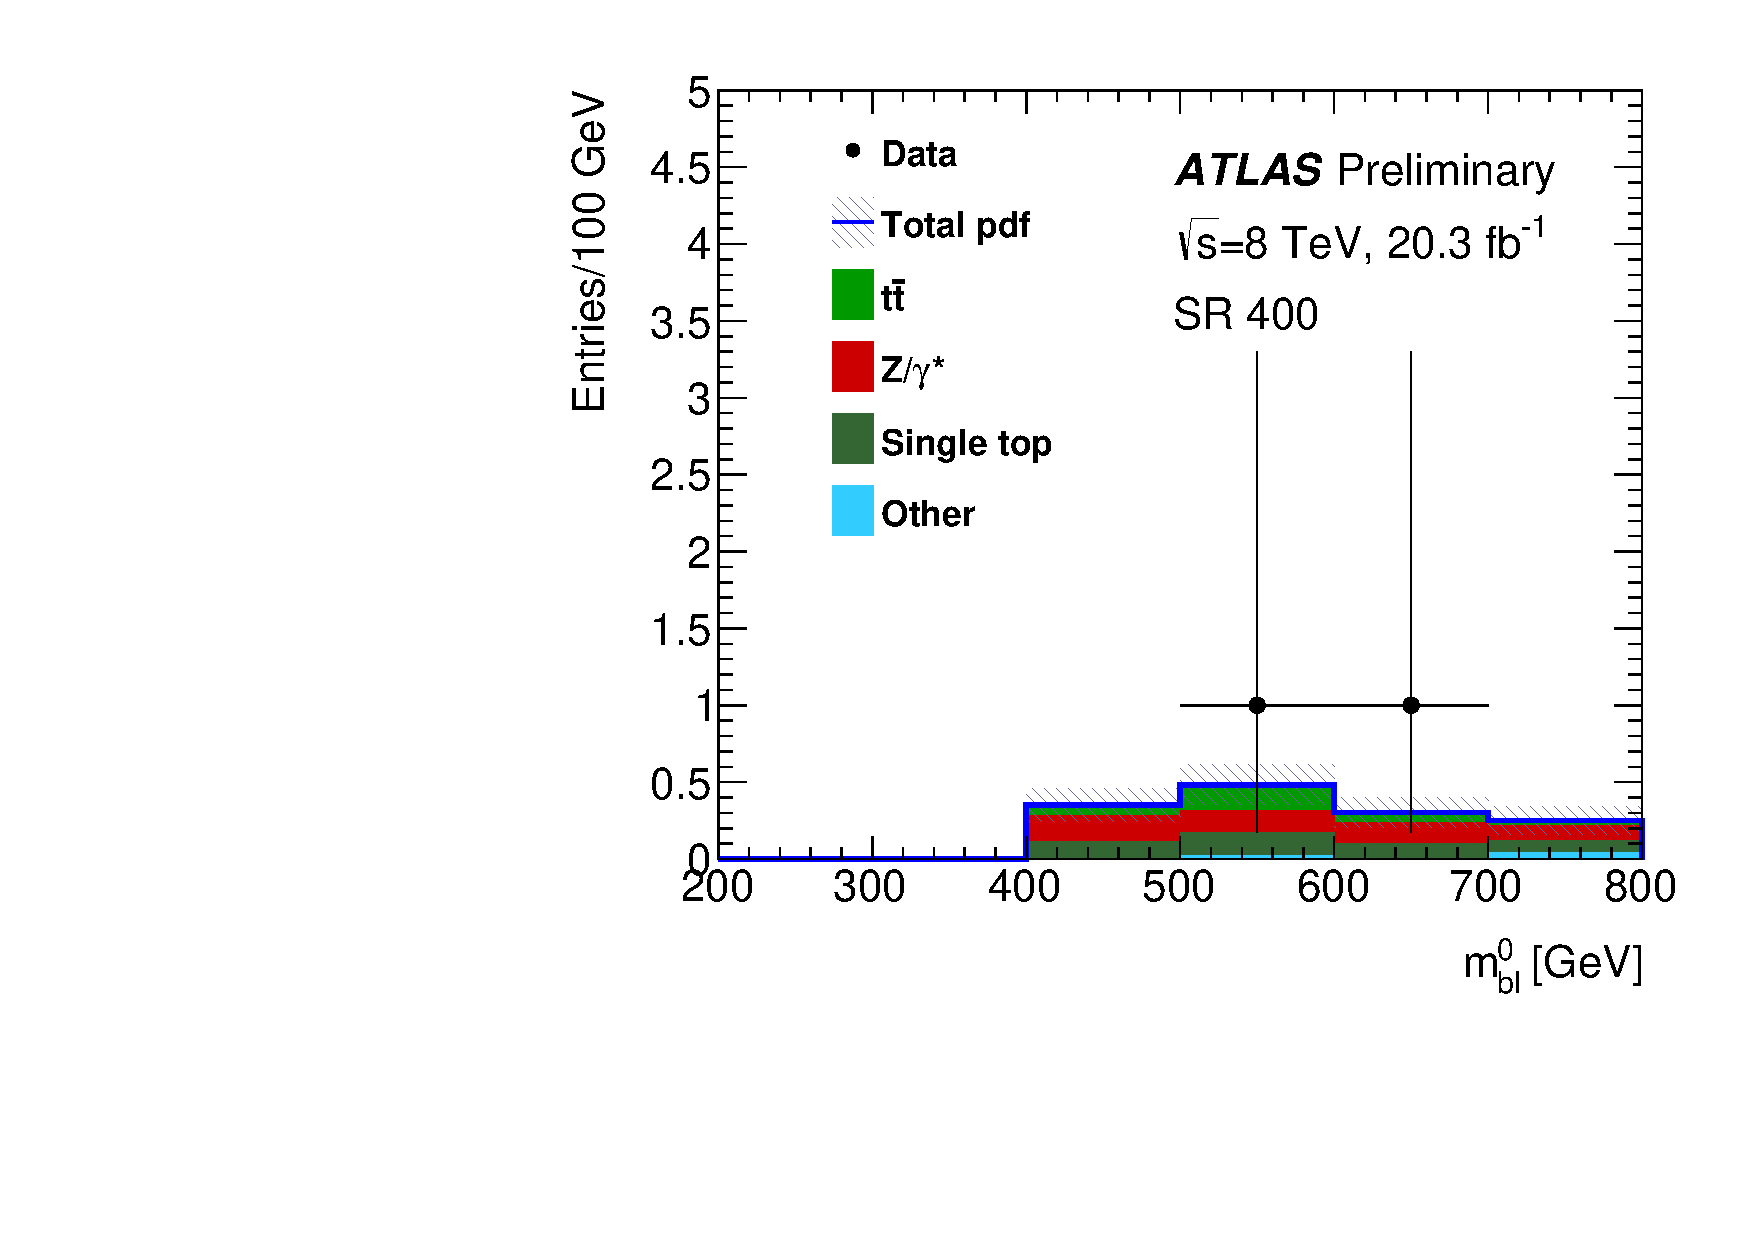
\includegraphics[width=0.75\textwidth]{figs/blstop/sr_mbl_0.pdf}
    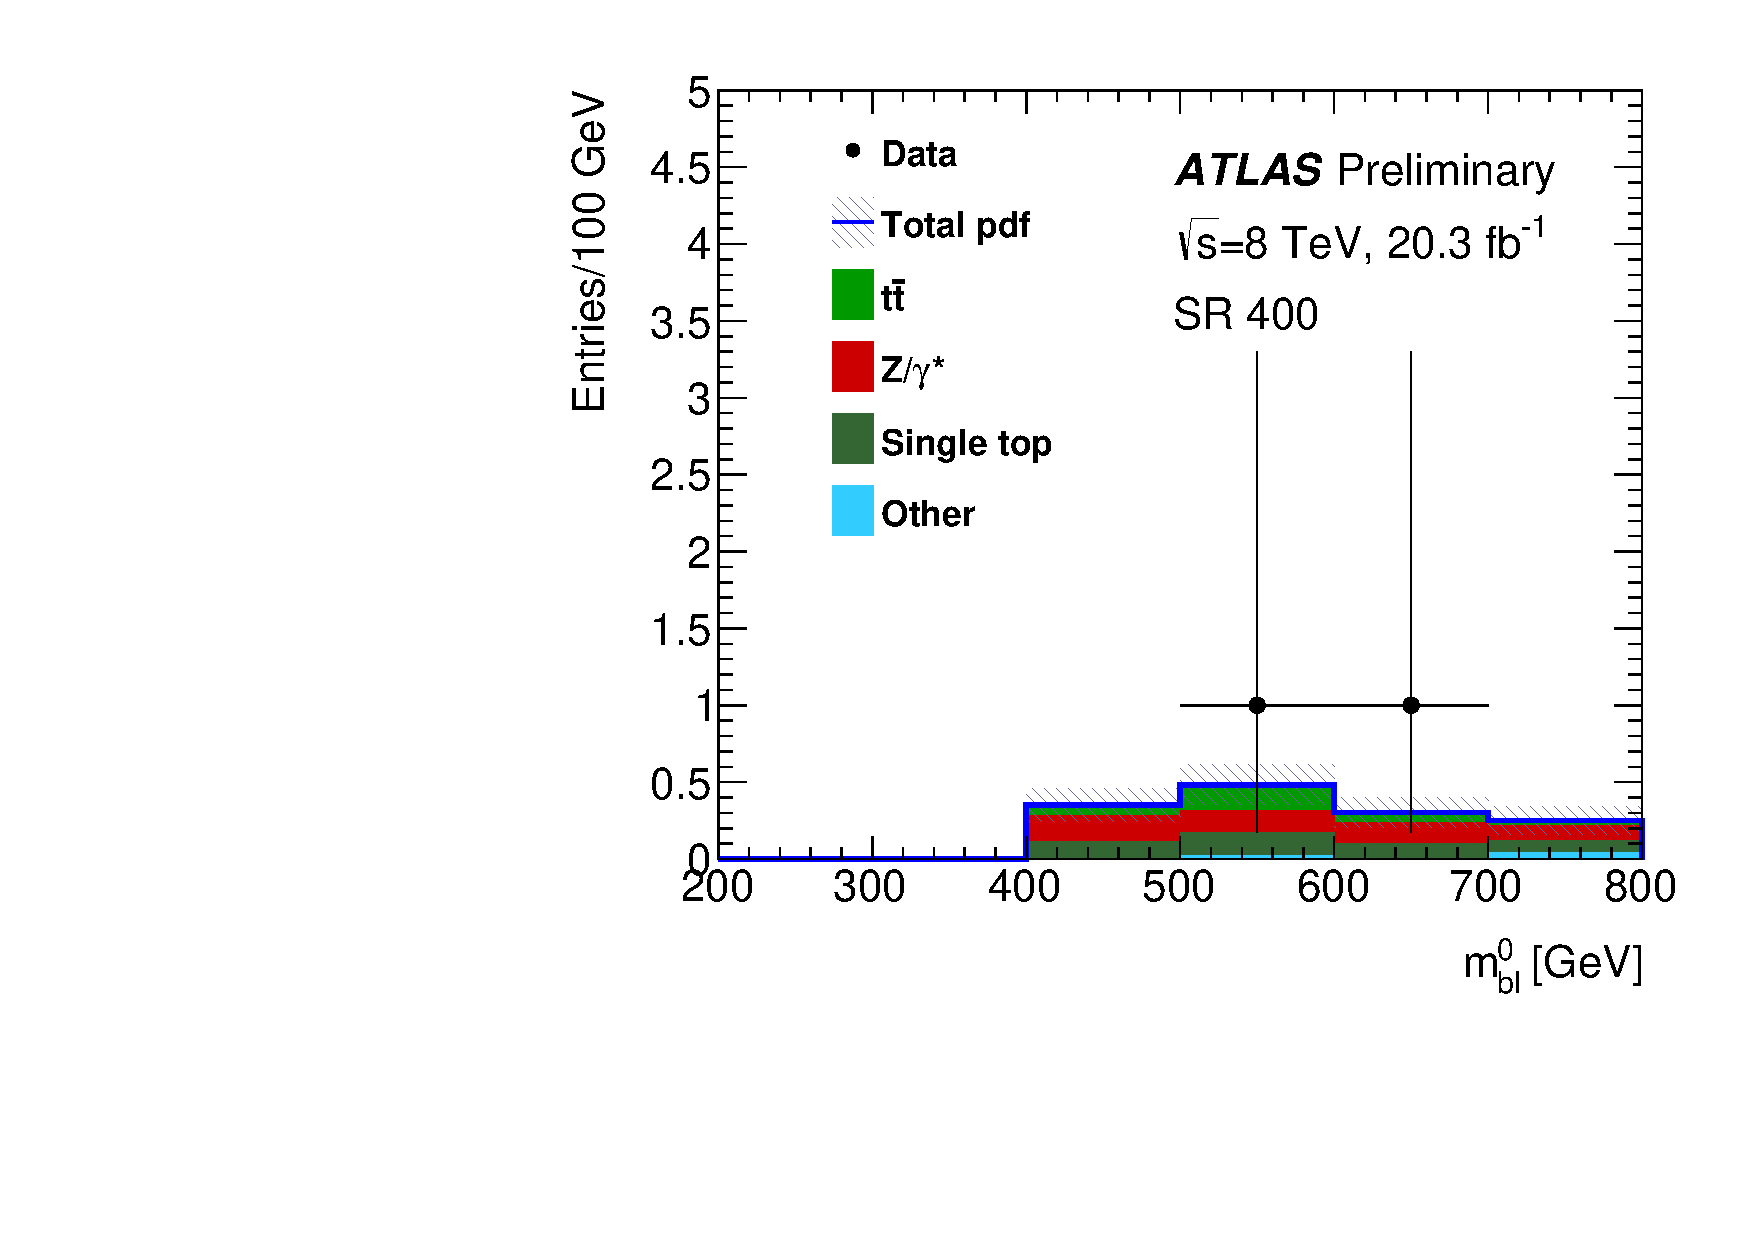
\includegraphics[width=0.70\textwidth]{figs/blstop/sr_mbl_0.pdf}
  }
  \subbottom[\HT]{
    % 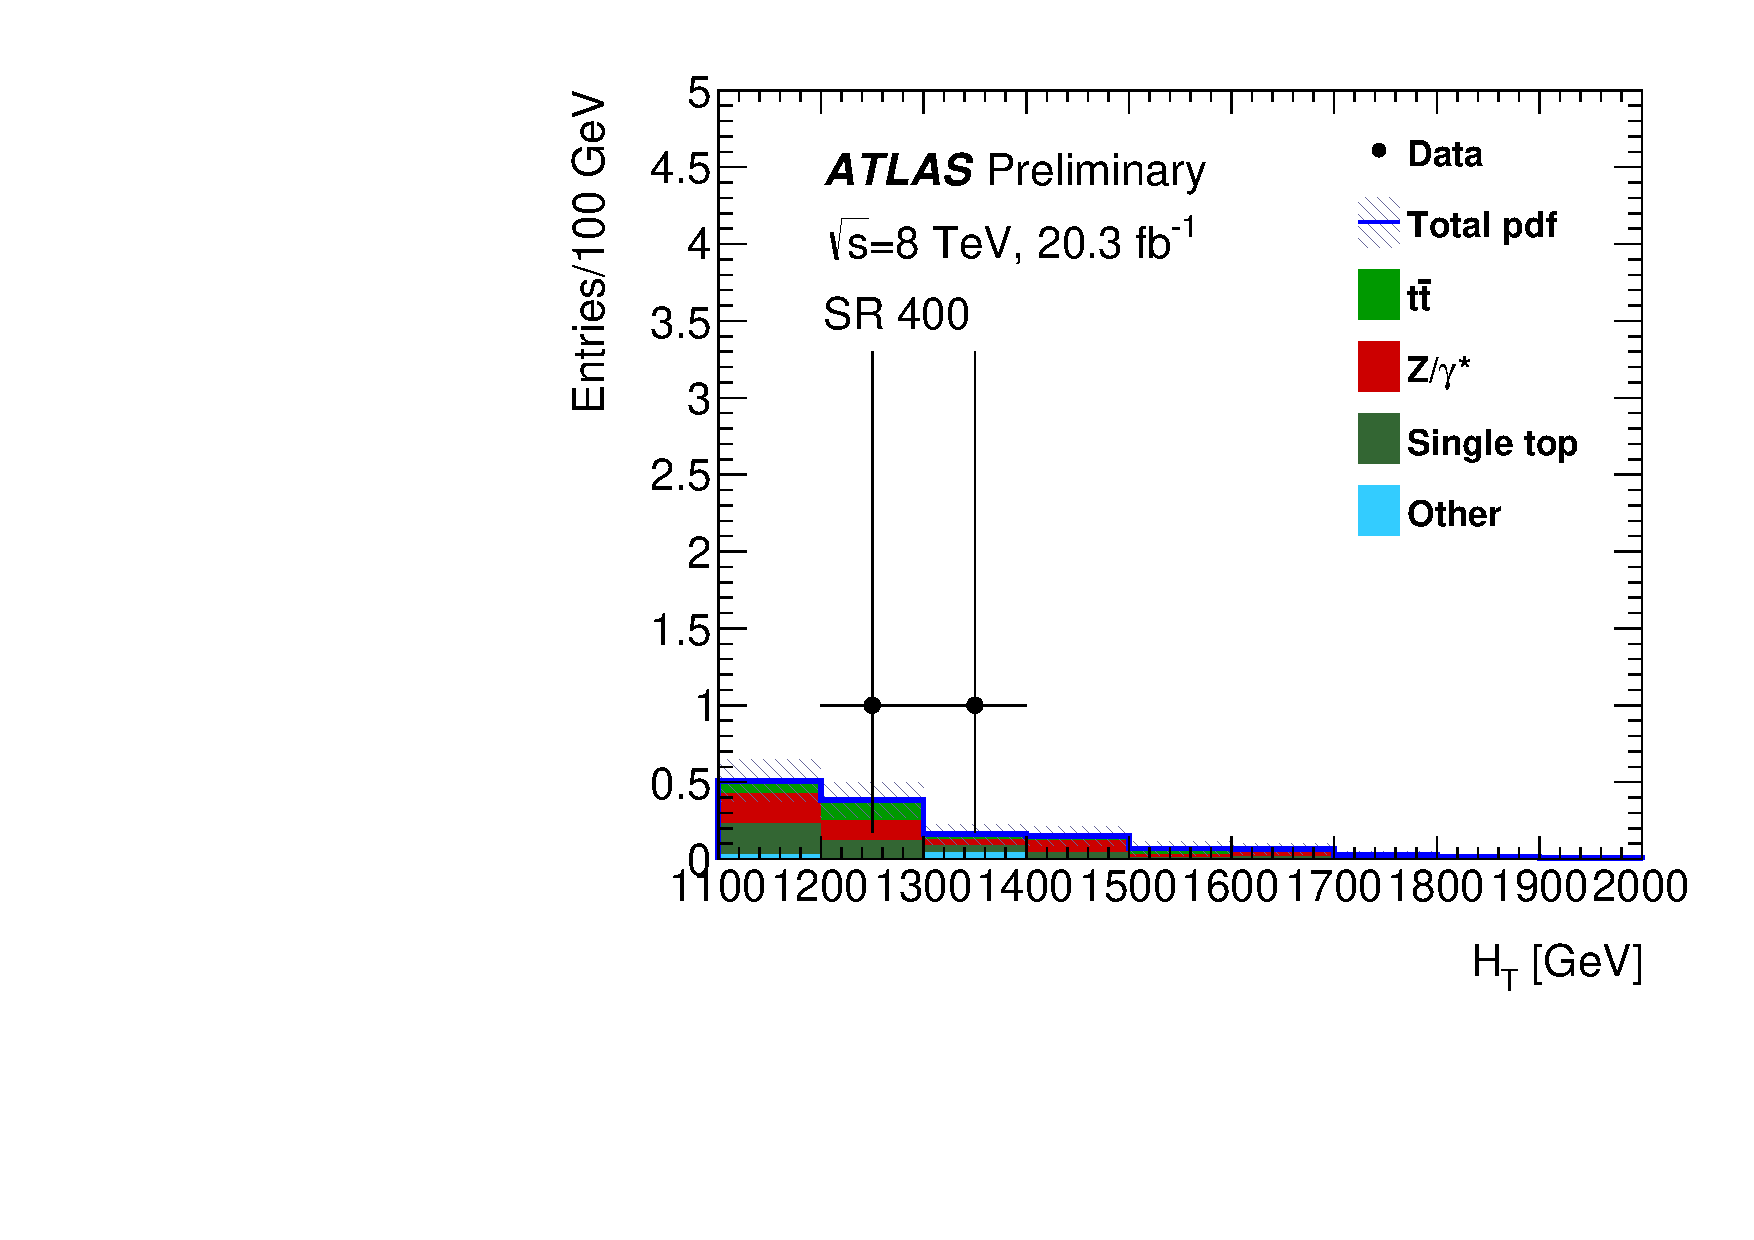
\includegraphics[width=0.75\textwidth]{figs/blstop/sr_ht.pdf}
    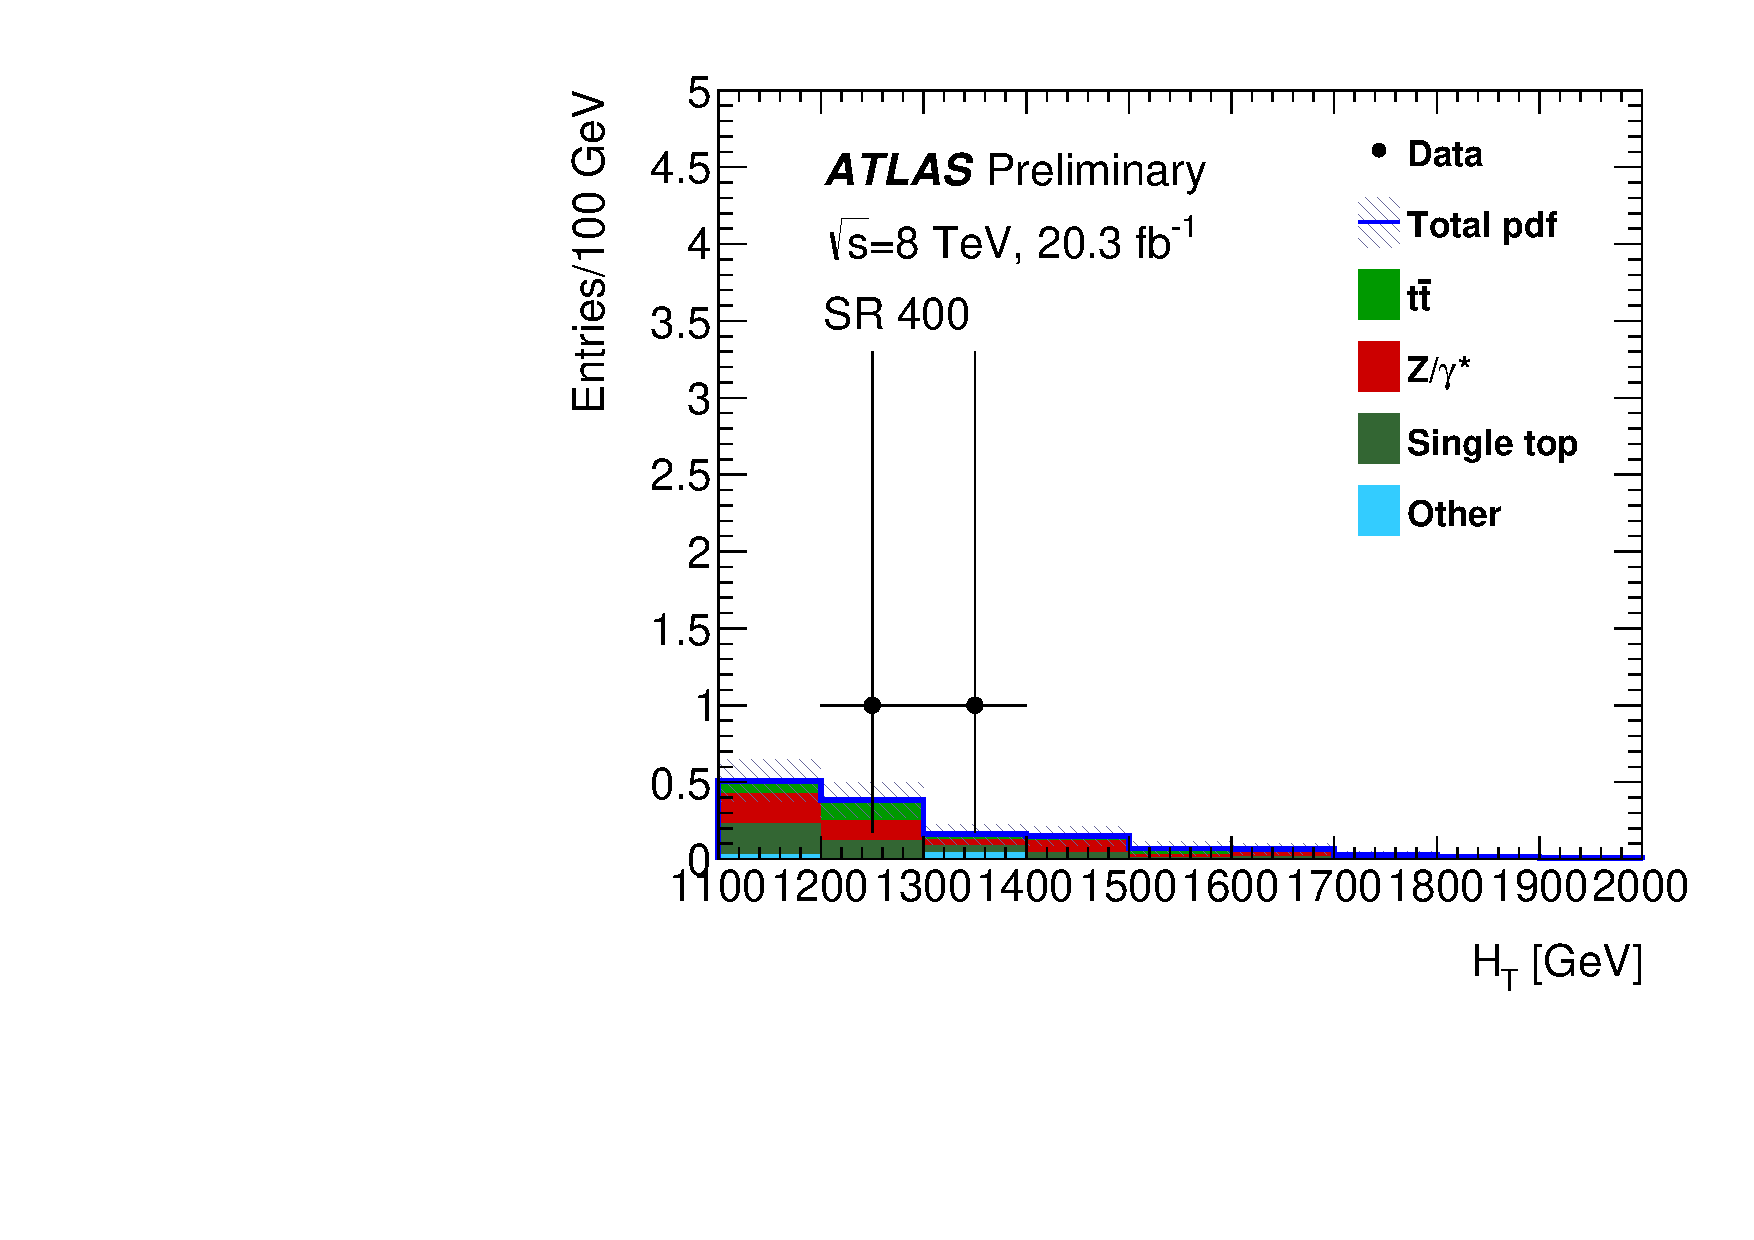
\includegraphics[width=0.70\textwidth]{figs/blstop/sr_ht.pdf}
  }
  \caption{These plots show the $\MBL^0$ (left) and \HT\ (right) distributions
    in SR 400.
    The Standard Model background prediction is taken from the fitted
    background prediction.
    The hashed bands show the uncertainty in the fitted background prediction
    including the MC statistical and sources of systematic uncertainty.
  }
  \label{fig:sr_dists}
\end{figure}

\begin{figure}[p]
  \centering
  \subbottom[Run 214216, Event 121272046]{
    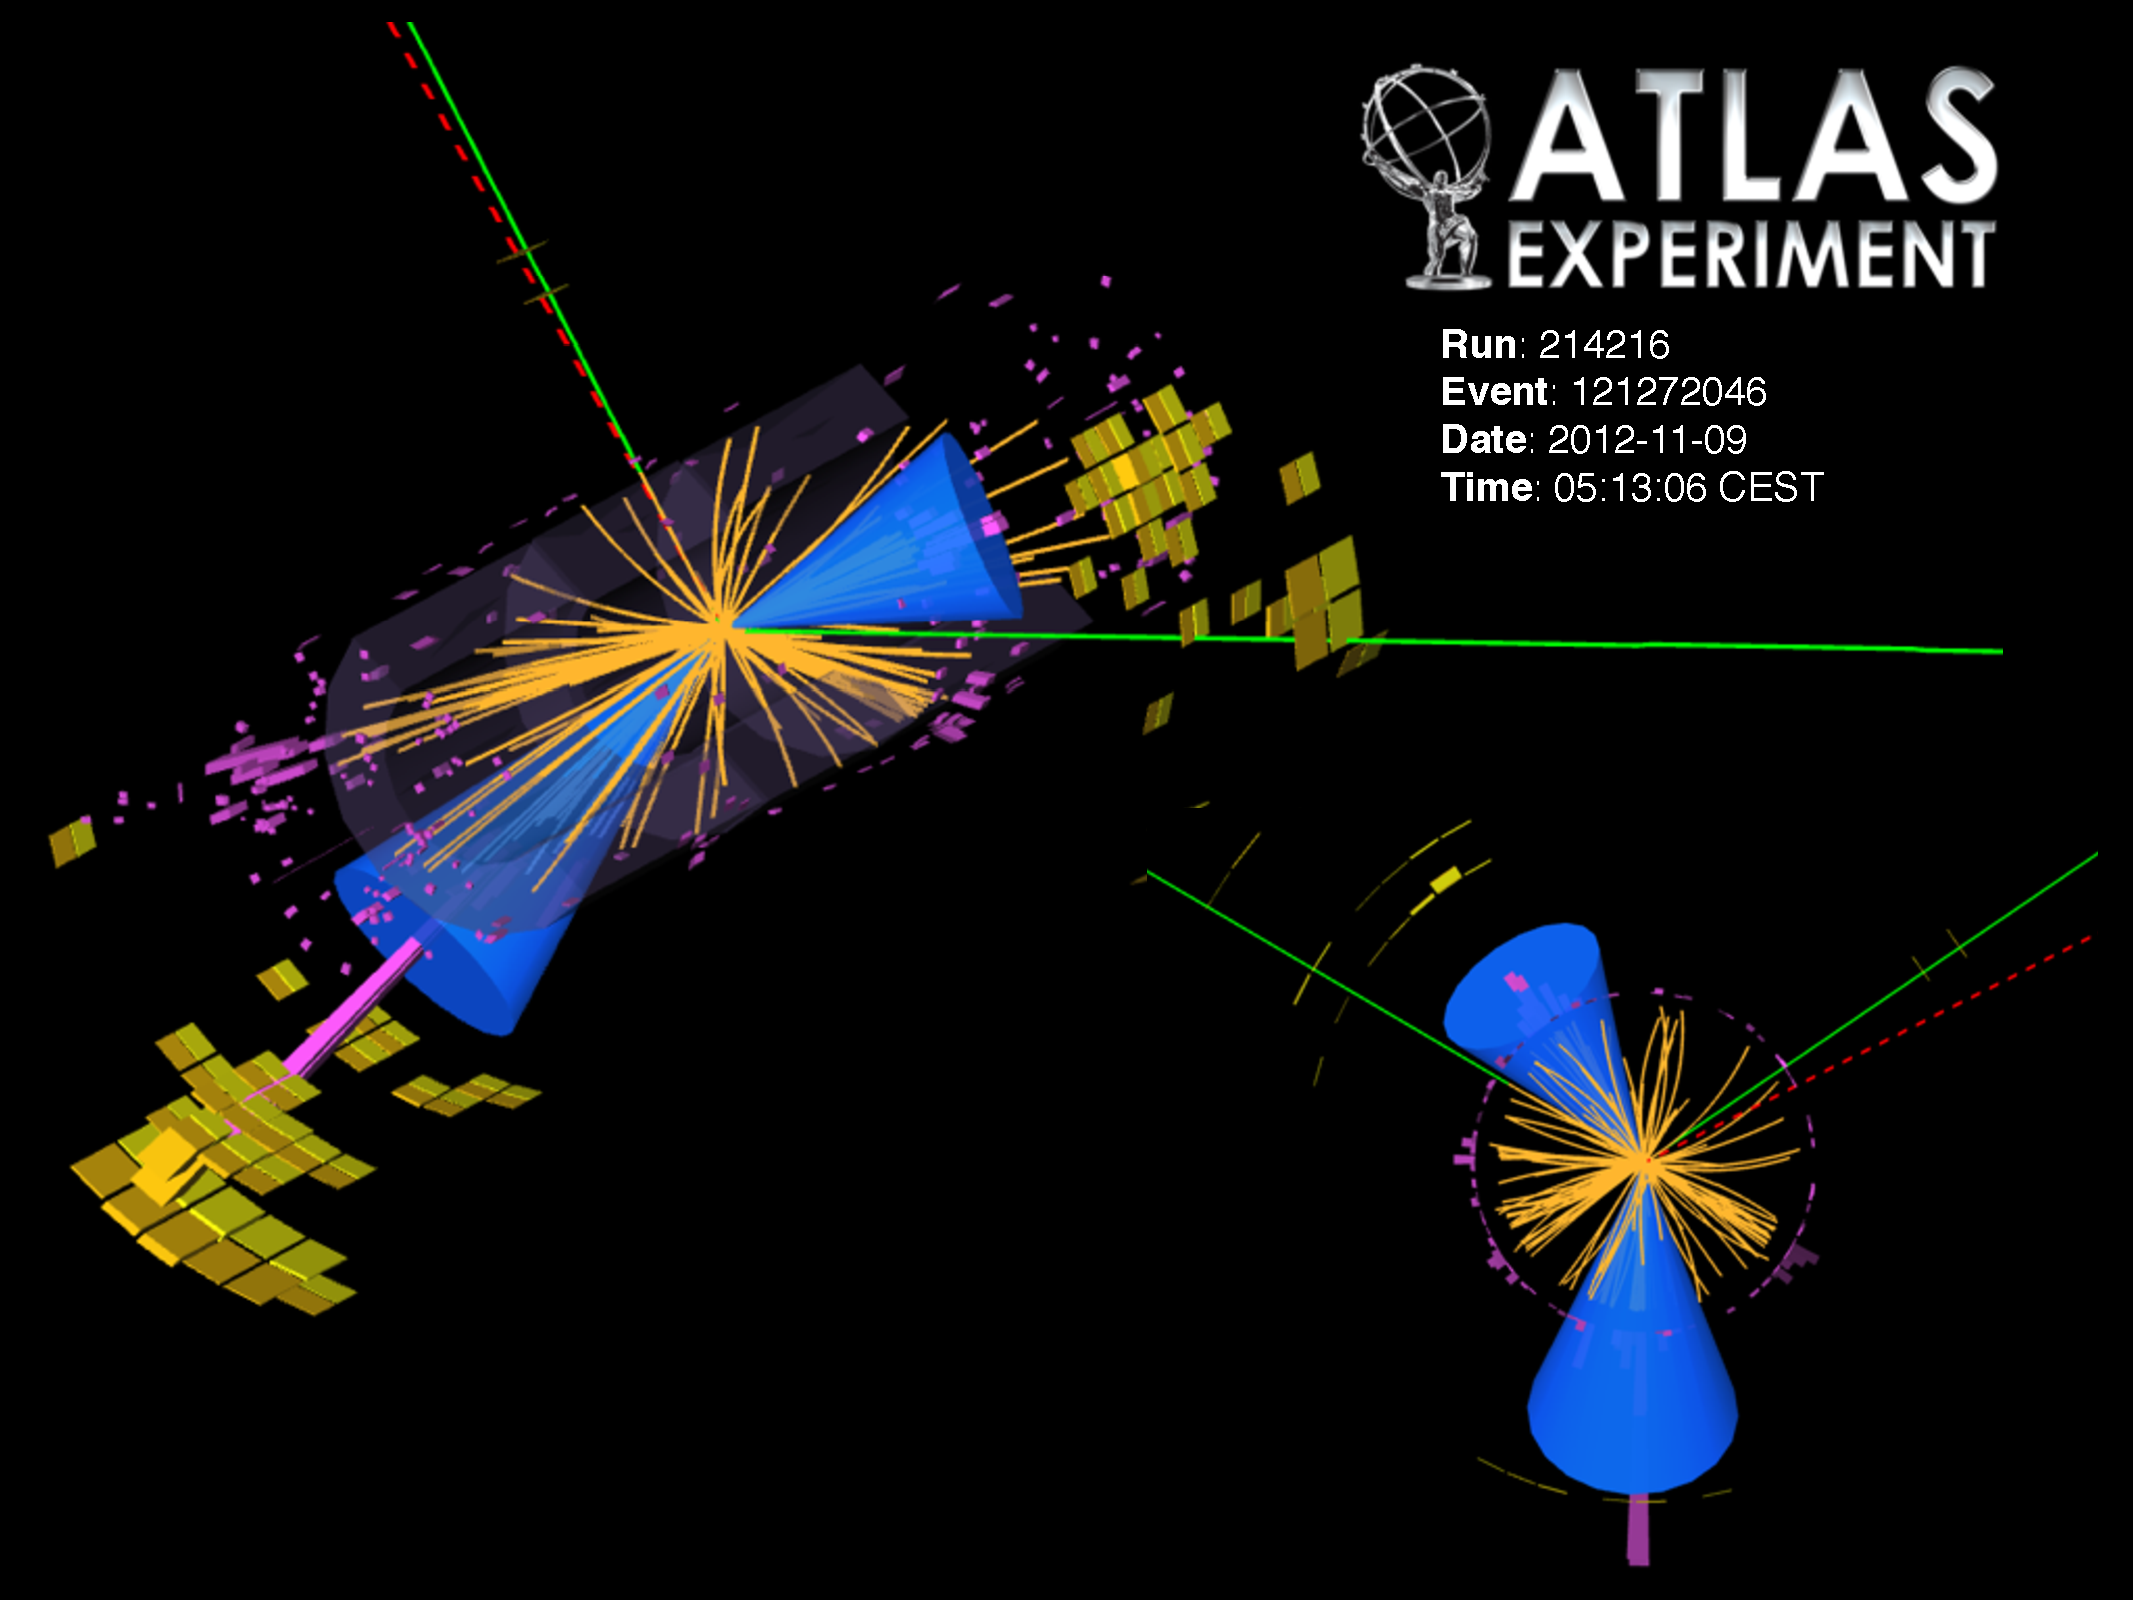
\includegraphics[height=0.41\textheight]
    {figs/blstop/event_display_run_214216_event_121272046.pdf}
    \label{fig:event_display_1}
  }
  \subbottom[Run 210302, Event 2292645761]{
    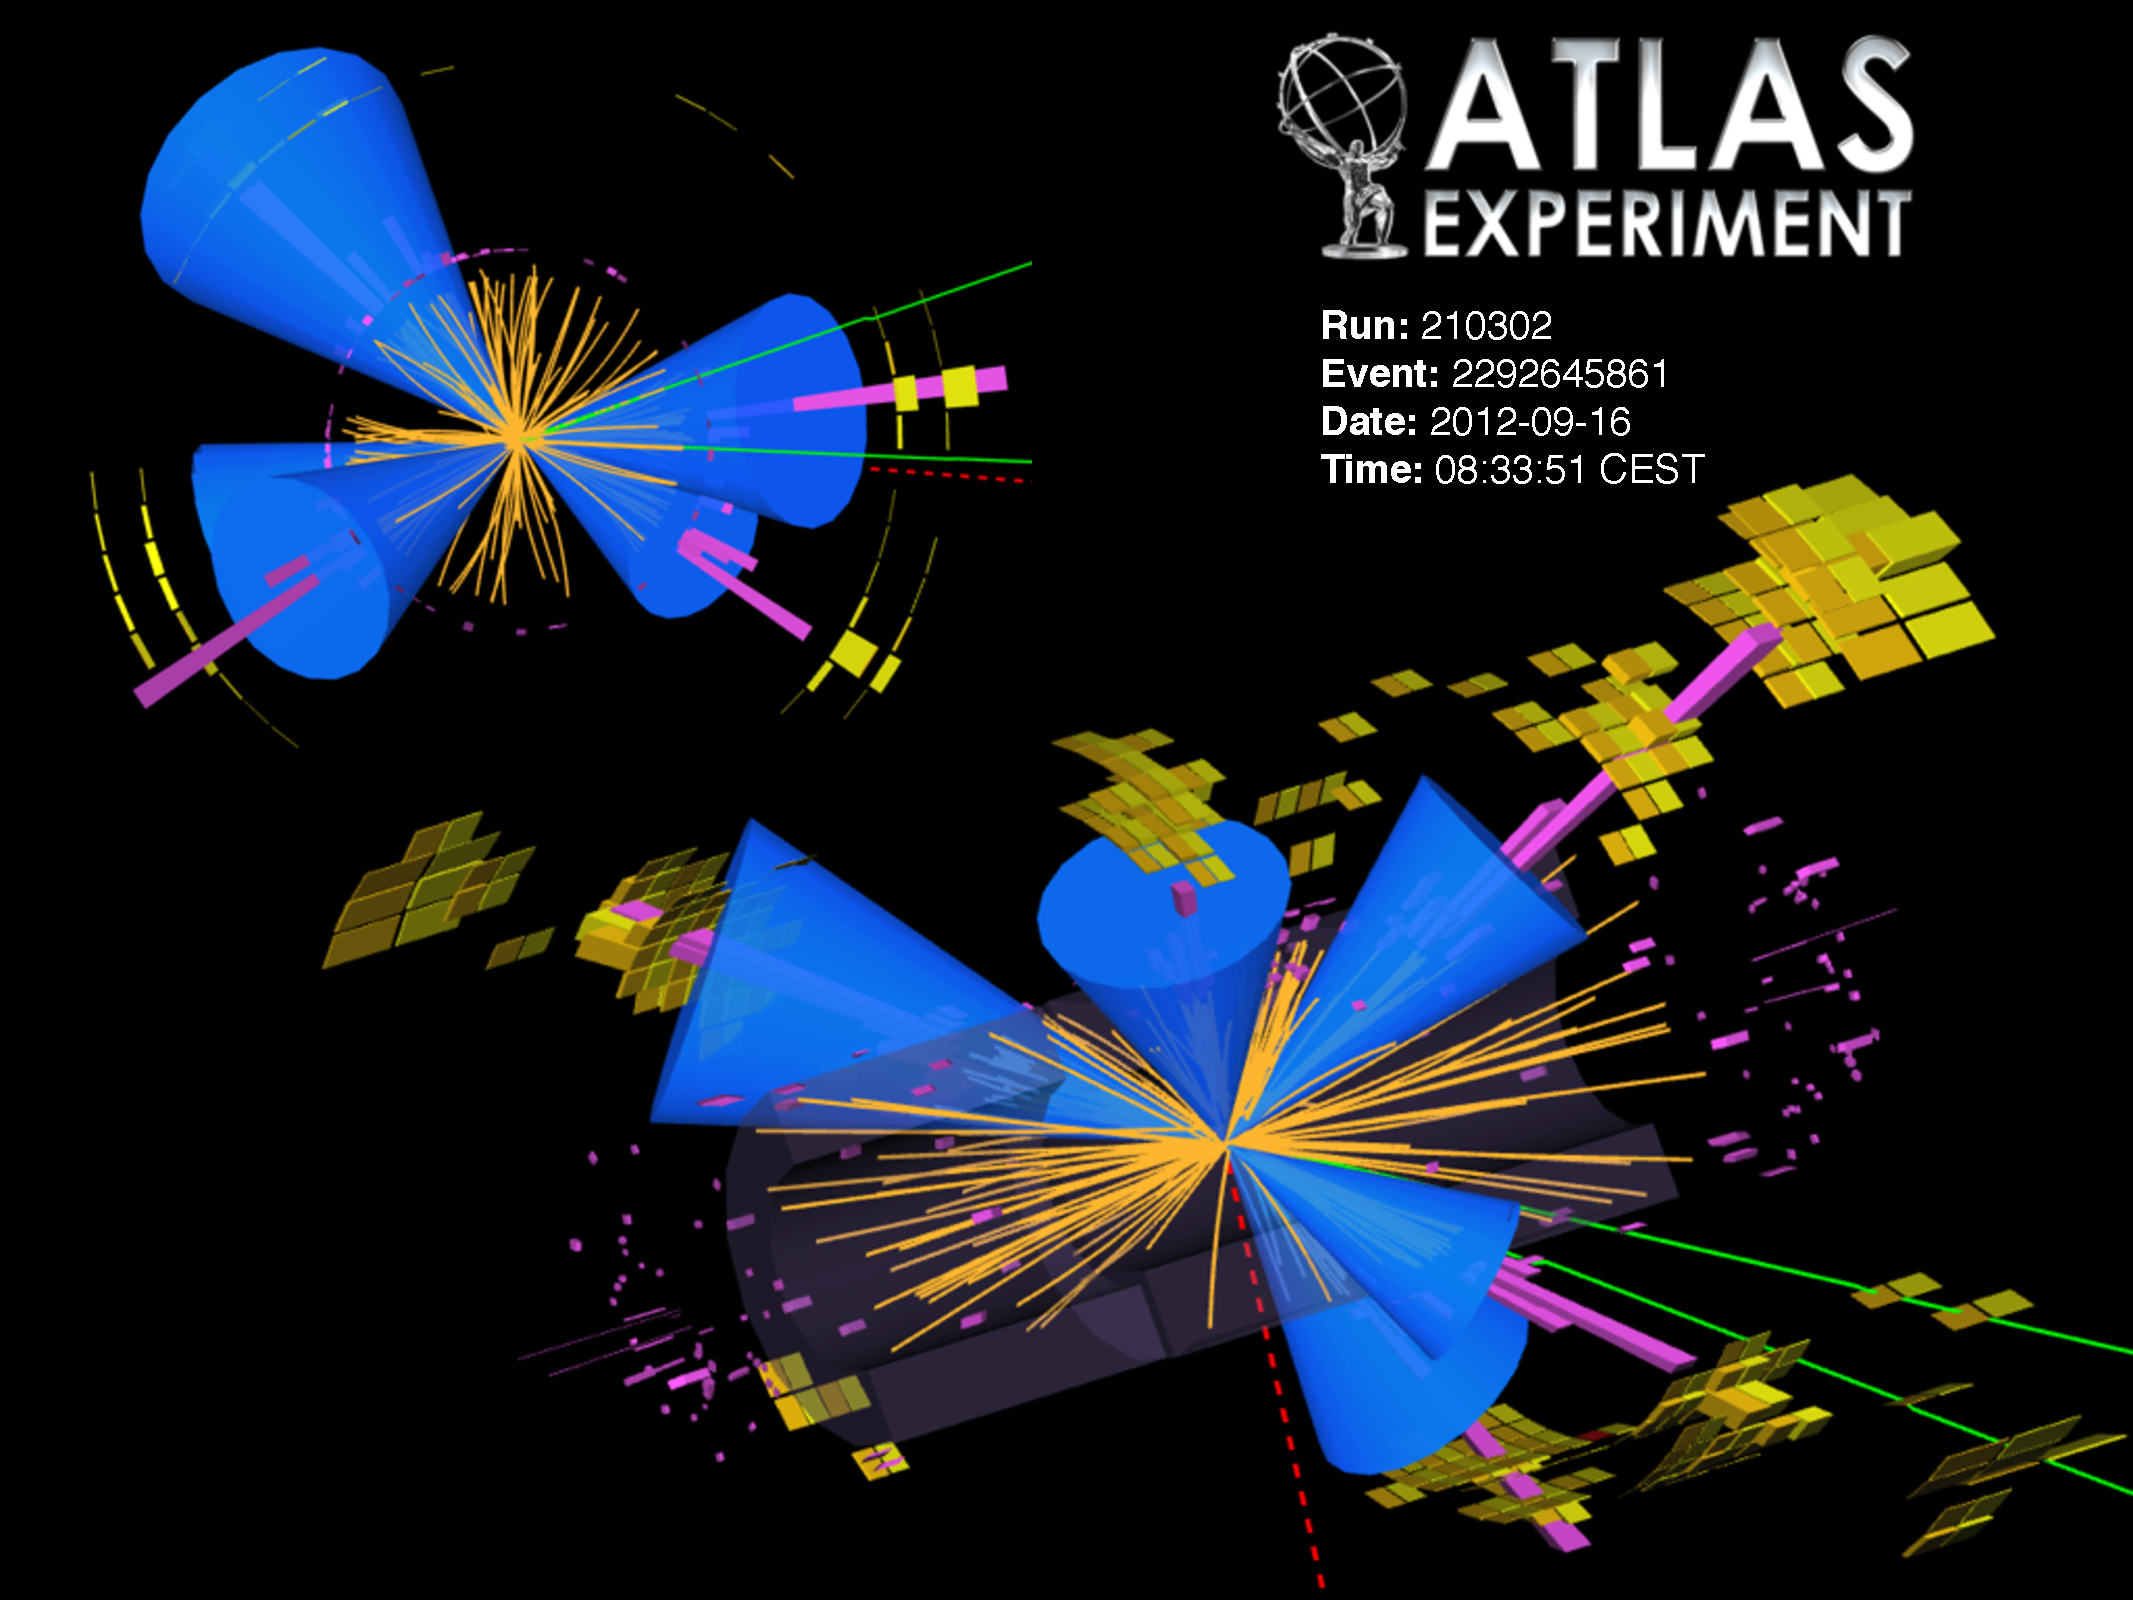
\includegraphics[height=0.41\textheight]
    {figs/blstop/event_display_run_210302_event_2292645761.pdf}
    \label{fig:event_display_2}
  }
  \caption{Event displays for the two observed events passing the signal region
    criteria.
    The event shown in Figure~\ref{fig:event_display_1} passes the SR~400
    selection with $\MBL^{0} = 558~\GeV$.
    Figure~\ref{fig:event_display_2} shows the event which passes both the
    SR~400 and SR~600 selection with $\MBL^{0} = 686~\GeV$.
  }
  \label{fig:event_displays}
\end{figure}

As the observed number of events is consistent with the SM
prediction, upper limits at 95\% confidence level (CL) on the number of
beyond the Standard Model (BSM) events for each signal region are derived
using the $CL_S$ prescription and neglecting any possible contamination in the
control regions~\cite{Baak:2014wma}.
Normalizing these by the integrated luminosity of the data sample they can be
interpreted as upper limits on the visible BSM cross section,
$\sigma_\mathrm{vis}$, where $\sigma_\mathrm{vis}$ is defined as the product of
acceptance, reconstruction efficiency and production cross section.
The model independent limits are given in
Tables~\ref{tab:event_yields_sr_400}~(SR 400)
and~\ref{tab:event_yields_sr_600}~(SR 600), and are shown for each flavor
channel separately, and for the combined SRs which sum over the three flavor
channels.
Since the two observed events are in the $\mu\mu$ channel, the limit on
$\sigma_\mathrm{vis}$ is stronger than expected in the $ee$ and $e\mu$
channels, and weaker than expected in the $\mu\mu$ channel.

%% -----------------------------------------------------------------------------
\FloatBarrier
\section{Model dependent limits}
\label{sec:model_dependent_limits}

In the absence of an excess of events in the SRs beyond the SM prediction,
limits are set on the allowable stop masses and branching fractions for this
model.
Expected and observed exclusion limits on the signal model are determined using
the $CL_S$ prescription based on a simultaneous fit of the SRs and
CRs~\cite{Baak:2014wma}.
The predicted small signal contamination in the CRs is taken into account for
each signal model tested.
An expected and observed mass limit is first determined for a single choice of
stop branching fraction, $Br(\tilde{t} \to eb) = Br(\tilde{t} \to \mu b) = 0.5$,
the nominal branching fraction simulated in the MC signal models.
Then, the simulated signal samples are rescaled in order to determine mass
limits for different choices of stop branching fractions.

%% -----------------------------------------------------------------------------
\FloatBarrier
\subsection{Single mass limit}
\label{sec:single_mass_limit}

Each SR (SR 400 and SR 600) is interpreted separately, using the predicted and
observed event yields in the CRs and the SR of interest.
A maximum likelihood fit is performed to obtain the model-dependent estimate of
the background and signal strengths.
When calculating the expected limit, the data in the SR is replaced with the
pre-fit MC prediction.
An expected and observed $CL_S$ value is computed for each simulated stop mass,
in each SR to assess the relative compatibility of the data with the
signal~+~background hypothesis and the background only hypothesis.
For each stop mass, the SR which gives the best expected sensitivity, as
measured by the lower $CL_S$ value is selected, and used to interpret the model
at that mass.
The \texttt{HistFitter} package limits the precision of the $CL_S$ value
to $10^{-6}$; if the two SRs are affected by this cutoff, SR~400 is chosen by
convention.
This simplification is not expected to affect the final result, as these points
are far from the limit, where the expected $CL_S$ is 0.05.
If the observed $CL_S$ value in the selected SR is less than 0.05, the signal
model is rejected at 95\%~CL.
An observed (expected) limit on the stop mass is determined by taking the
highest stop mass, with an observed (expected) $CL_S$ value less than 0.05.
Figure~\ref{fig:exp_limit_br_5050} shows an example $CL_S$ plot (both SRs)
for the scenario with $Br(\tilde{t} \to eb) = Br(\tilde{t} \to \mu b) = 0.5$.
In the high mass regime, SR~600 is selected to interpret the mode, and
the points where the solid line is below 0.05 (indicated with a dashed red line)
are excluded.
No interpolation between the mass points is performed, so the mass limit for
this choice of stop branching fractions is 900~\GeV.

\begin{figure}[t]
  \centering
  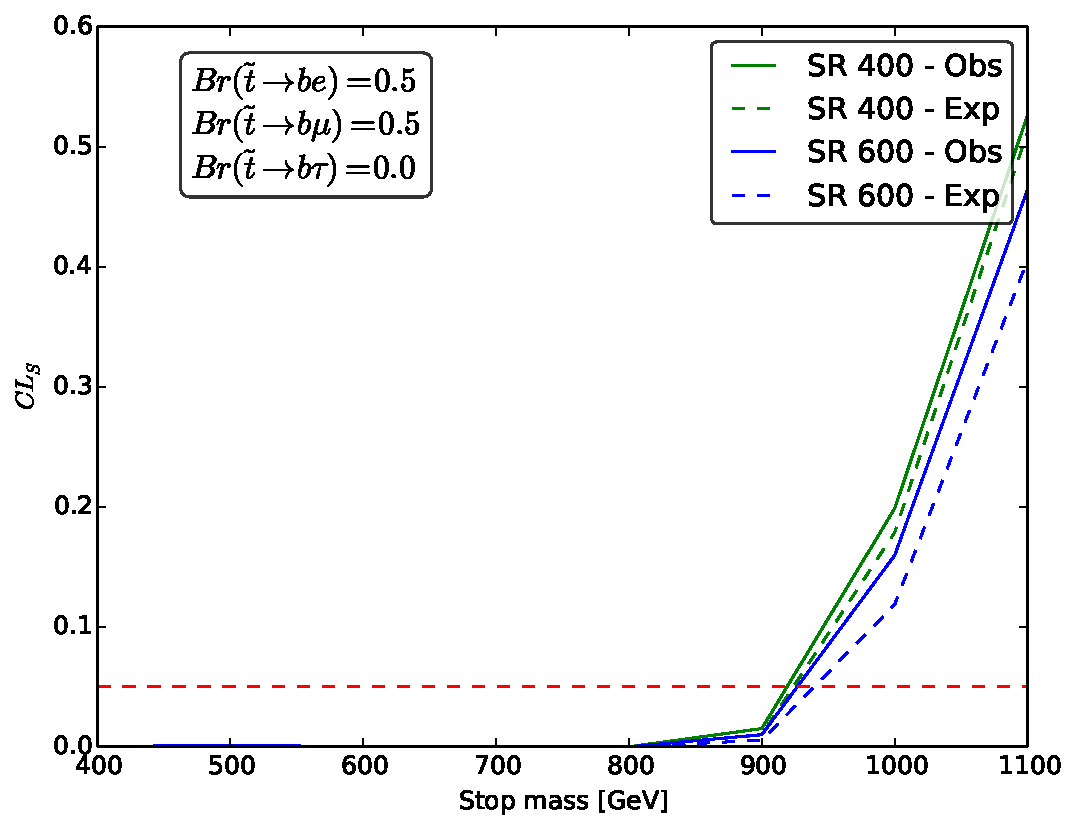
\includegraphics[width=0.75\textwidth]{figs/blstop/cls_plots/cls_vs_m_br_e_50_br_m_50_br_t_0.pdf}
  \caption{Expected and observed $CL_S$ value as a function of stop mass for
    the scenario with $Br(\tilde{t} \to eb) = Br(\tilde{t} \to \mu b) = 0.5$.
    The last mass which has an observed $CL_S < 0.05$ is where the limit is to
    be set.
    {\color{red} TODO remake with ATLAS Internal on plots and add marker where
    tested stop masses are}
  }
  \label{fig:exp_limit_br_5050}
\end{figure}

%% -----------------------------------------------------------------------------
\FloatBarrier
\subsection{Branching fraction scan}
\label{sec:branching_fraction_scan}

This procedure of finding a stop mass limit is repeated for branching fractions
across the plane of allowed values.
The MC simulation stop samples are generated with fixed branching
fractions of $Br(\stop \to be) = Br(\stop \to b\mu) = 0.5$, however, an
additional event weight is constructed to scale the simulated signal
process to the desired choice of stop branching fraction.
This event weight depends on the lepton flavor channel of each MC simulated
event.
% It was shown that the disagreement between the generated and reconstructed
% flavor channels is negligible, so the reconstructed di-lepton flavor channel
% is used to select the additional weight.

For a choice of stop branching fraction, the di-stop branching fractions are
given by 
\begin{equation}
  \label{eqn:branching_fractions}
  \begin{aligned}
    Br_\mathrm{flavor}(\tilde{t}\tilde{t}^{*} \rightarrow bbee)     &=
      Br_\mathrm{flavor}(\tilde{t} \rightarrow be )^{2} \\
    Br_\mathrm{flavor}(\tilde{t}\tilde{t}^{*} \rightarrow bb\mu\mu) &=
      Br_\mathrm{flavor}(\tilde{t} \rightarrow b\mu )^{2} \\
    Br_\mathrm{flavor}(\tilde{t}\tilde{t}^{*} \rightarrow bbe\mu)   &=
      2Br_\mathrm{flavor}(\tilde{t} \rightarrow be )
      Br_\mathrm{flavor}(\tilde{t} \rightarrow b\mu ).
  \end{aligned}
\end{equation}

The di-stop branching fractions for each flavor channel are plotted for choices
of the single-stop branching fraction in Figure~\ref{fig:flavor_scaling_bf},
where darker colors represent a higher branching fraction.
The simulated stop samples correspond the center of the $x$-axis, and have
di-stop branching fractions of 0.25, 0.25, and 0.50 for the $eebb$,
$\mu\mu bb$, $e\mu bb$ channels respectively.
As the value of $Br(\tilde{t} \to be)$ increases (represented by moving toward
the bottom right corner of each of the plots), the fraction of events decaying
to the $eebb$ final state increases, while the other two flavor channels
have fewer expected events.
Similarly, as the value of $Br(\tilde{t} \to b\mu)$ increases (represented by
moving toward the bottom left corner of each of the plots), the fraction of
events decaying to the $\mu\mu bb$ final state increases.
Finally, increasing branching fraction of the $\tilde{t} \to b\tau$ decay
(represented by moving toward the upper left corner of the plots) results in a
decreasing number of expected events with two light leptons.

\begin{figure}[ht]
  \centering
  \subbottom[Stop branching fractions for each flavor channel]{
    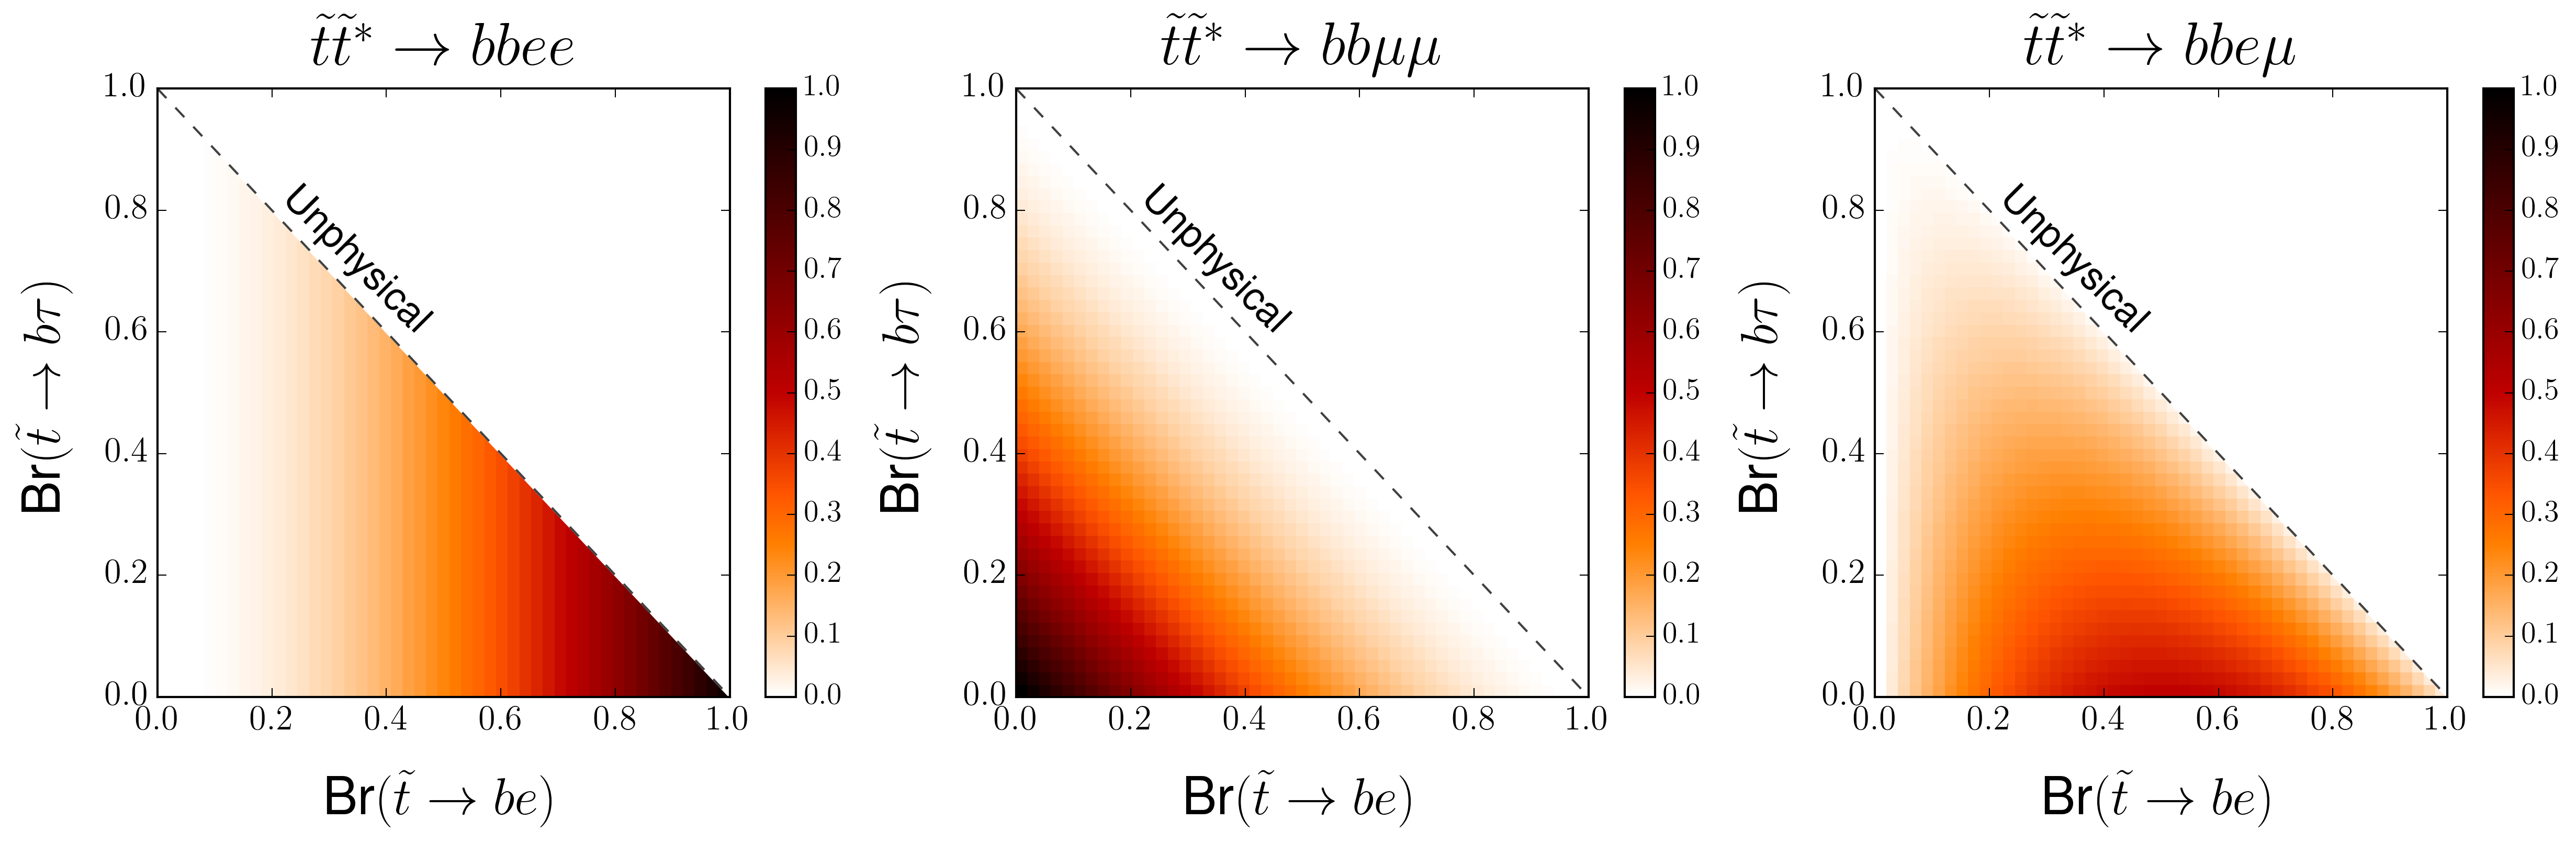
\includegraphics[width=\textwidth]{figs/blstop/branching_fractions.png}
    \label{fig:flavor_scaling_bf}
  }
  \subbottom[Scale factors for each flavor channel]{
    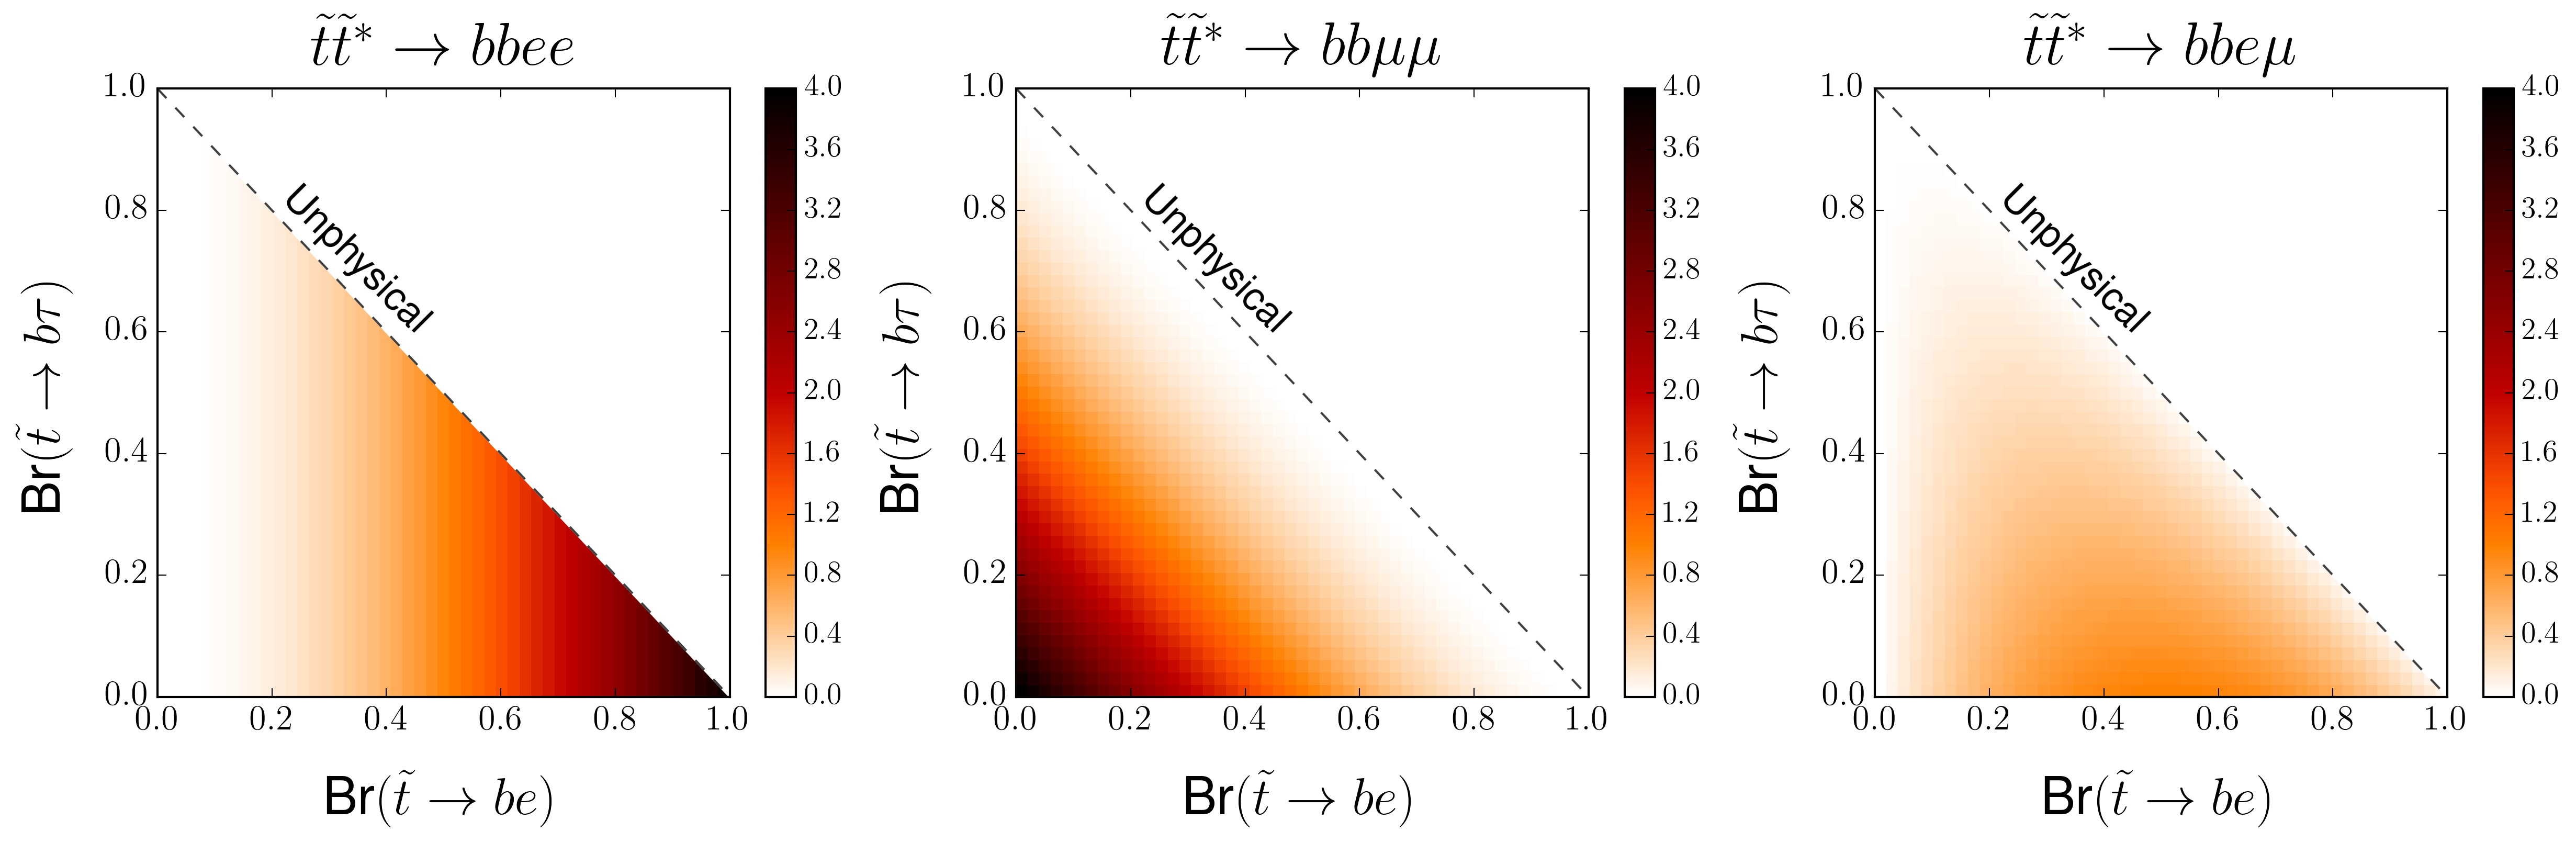
\includegraphics[width=\textwidth]{figs/blstop/scale_factors.png}
    \label{fig:flavor_scaling_sf}
  }
  \caption{Branching fraction and corresponding scale factor to each di-lepton
    flavor channel depending on the branching fractions of the stop.
    The di-stop branching fractions are given by
    Equation~\ref{eqn:branching_fractions}.
    The scale factor plot obtained by plotting
    Equation~\ref{eqn:flavor_scale_factor}.
    In all six plots, a darker color corresponds to a higher value for the
    branching fraction or the scale factor.
    % {\color{red} TODO Do I want to keep this scale factor plot in here? It's
    % just a rescaling of the branching fraction plot, so it may not add
    % anything.
    % }
  }
  \label{fig:flavor_scaling}
\end{figure}

Taking the ratio of the target and nominal di-stop branching fraction, a
scale factor is defined for each flavor channel to weight the MC simulation
such that it can represent any stop branching fraction.
These scale factors are given by
\begin{equation}
  \label{eqn:flavor_scale_factor}
  \begin{aligned}
    SF_\mathrm{flavor}(\tilde{t}\tilde{t}^{*} \rightarrow bbee)     &=
      \frac{Br(\tilde{t} \rightarrow be)^2}{0.25} \\
    SF_\mathrm{flavor}(\tilde{t}\tilde{t}^{*} \rightarrow bb\mu\mu) &=
      \frac{Br(\tilde{t} \rightarrow b\mu)^2}{0.25} \\
    SF_\mathrm{flavor}(\tilde{t}\tilde{t}^{*} \rightarrow bbe\mu)   &=
      \frac{2Br(\tilde{t} \rightarrow be)Br(\tilde{t} \rightarrow b\mu)}{0.50}.
  \end{aligned}
\end{equation}
The appropriate flavor scale factor is applied to each simulated signal event
depending on the reconstructed flavor channel.
The values of the scale factors are shown in Figure~\ref{fig:flavor_scaling_sf},
where a darker color corresponds to a larger value for the scale factor (with a
maximum value of 4).

The expected and observed $CL_S$ values in SR~400 and SR~600 are shown
over a range of stop branching fraction hypotheses in
Figures~\ref{fig:cls_plane_sr_400_m_500} and~\ref{fig:cls_plane_sr_600_m_900}
respectively for select stop masses of 500 \GeV\ and 900 \GeV.
A complete collection of the expected and observed $CL_S$ plots are found in
Appendix~\ref{sec:axp_interpretation_plots}.

% \begin{figure}[ht]
\begin{figure}[p]
  \centering
  \subbottom[Expected $CL_S$ or SR~400]{
    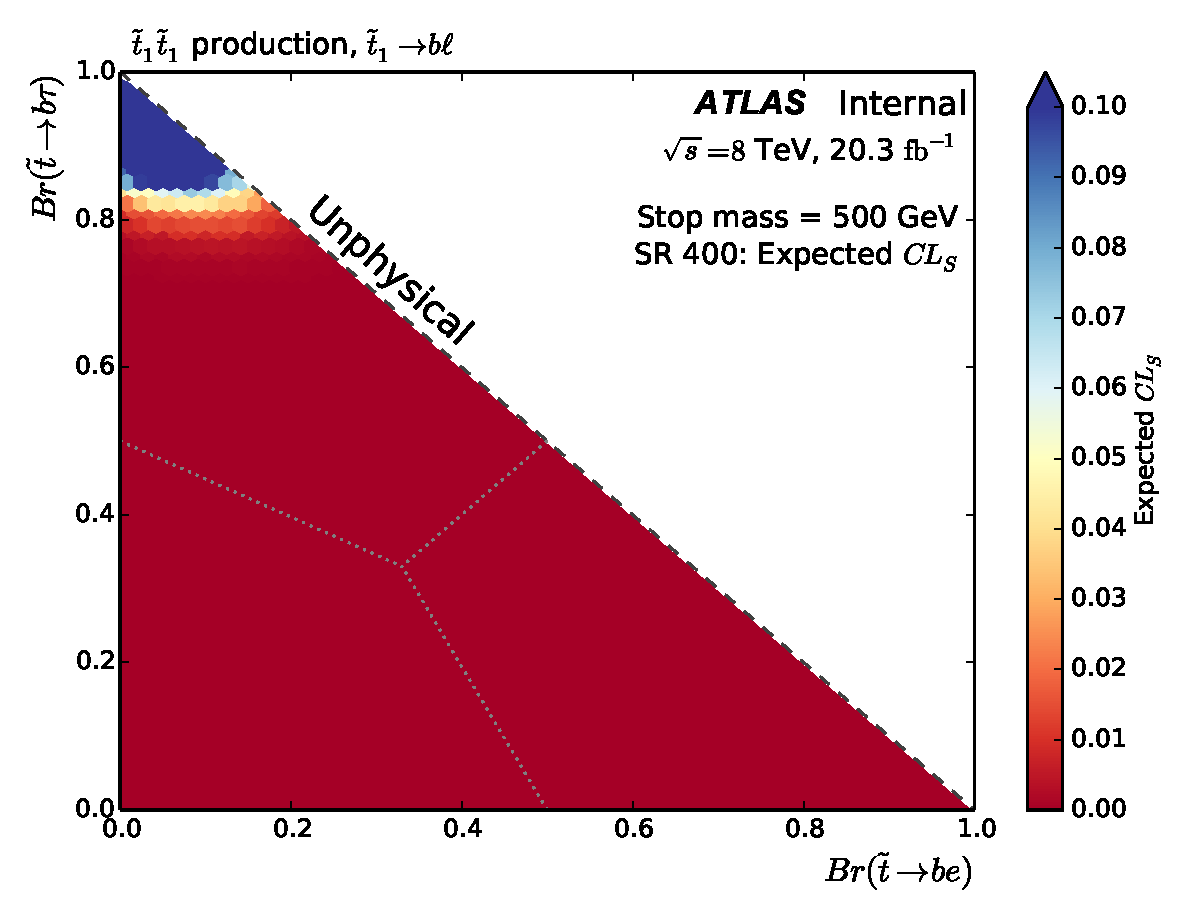
\includegraphics[width=0.48\textwidth]
      {figs/blstop/cls_plots/cls_vs_br_m_500_sr_400_exp.pdf}
  }
  \subbottom[Observed $CL_S$ or SR~400]{
    \includegraphics[width=0.48\textwidth]
      {figs/blstop/cls_plots/cls_vs_br_m_500_sr_400_obs.pdf}
  }
  \caption{
    The expected and observed $CL_S$ values in SR~400 for a stop mass of
    500~\GeV, shown across the plane of physical stop branching fractions.
  }
  \label{fig:cls_plane_sr_400_m_500}
\end{figure}

% \begin{figure}[ht]
\begin{figure}[p]
  \centering
  \subbottom[Expected $CL_S$ or SR~600]{
    \includegraphics[width=0.48\textwidth]
      {figs/blstop/cls_plots/cls_vs_br_m_900_sr_600_exp.pdf}
  }
  \subbottom[Observed $CL_S$ or SR~600]{
    \includegraphics[width=0.48\textwidth]
      {figs/blstop/cls_plots/cls_vs_br_m_900_sr_600_obs.pdf}
  }
  \caption{
    The expected and observed $CL_S$ values in SR~600 for a stop mass of
    900~\GeV, shown across the plane of physical stop branching fractions.
  }
  \label{fig:cls_plane_sr_600_m_900}
\end{figure}

A limit on the allowed stop masses and stop branching fractions is obtained
similar to the example with a single branching fraction hypothesis.
For each combination of stop mass and branching fractions, the SR which gives
the lowest expected value of $CL_S$ is selected. The SR selection for select
masses are shown in Figure~\ref{fig:sr_selection}.
Based on the selected SR, the model is rejected at 95\% CL if the observed
$CL_S$ is less than 0.05, and for each branching fraction, the highest stop
mass which is excluded is taken to be the mass limit.

\begin{figure}[ht]
% \begin{figure}[p]
  \centering
  \subbottom[Selected SR for 500~Gev stop mass]{
    \includegraphics[width=0.48\textwidth]
      {figs/blstop/region_selection/region_choice_vs_br_m_500.pdf}
  }
  \subbottom[Selected SR for 900~Gev stop mass]{
    \includegraphics[width=0.48\textwidth]
      {figs/blstop/region_selection/region_choice_vs_br_m_900.pdf}
  }
  \caption{
    The selected SR for select stop branching fractions for a stop mass of
    500~\GeV (left) and 900~\GeV (right).
    The SR is selected by choosing the SR with the smallest expected $CL_S$
    value for a given branching fraction.
    % For several points in the branching fraction plane, SR~400 was selected because
    % the two regions have the same expected $CL_S$ value, with the numerical
    % precision of the statistical software.
    % For these points, the expected sensitivity for both SRs is such that
    % there is little difference between the expected sensitivity.
  }
  \label{fig:sr_selection}
\end{figure}

Figure~\ref{fig:mass_limit_exp} shows the expected 95\% CL mass limit for each
point on the stop branching fraction plane.
These limits are obtained by selecting the highest stop mass with an expected
$CL_S < 0.05$ in the selected SR.
For each point on the stop branching fraction plane, the color corresponds to the
maximum excluded stop mass or the selected branching fraction hypothesis.
The nominal stop cross section is used when determining these limit contours.

\begin{figure}[p]
  \centering
  \includegraphics[width=\textwidth]
    {figs/blstop/mass_limit_contours_no_extras_exp.pdf}
  \caption{The expected mass limit on the stop at 95\% CL.
    This limit is obtained using the nominal stop cross section.
    Stop masses between 400~\GeV\ and 1100~\GeV, in steps of 100~\GeV, are
    tested.
    The mass limit shown corresponds to the highest-mass stop sample which is
    excluded.
  }
  \label{fig:mass_limit_exp}
\end{figure}

The expected and observed limits for each stop mass are shown in
Figure~\ref{fig:limit_contours}.
This figure shows, for each simulated stop mass, the observed (expected)
95\% exclusion limit on the branching fraction under the red (blue) line.
A yellow band shows the $\pm 1\sigma$ uncertainty in the expected limit,
determined from the systematic uncertainty in the signal and background
prediction excluding the effect of the signal cross section uncertainty.
The effect of varying the signal cross section on the observed limit is
indicated by the dashed red lines.
Since the two observed events are in the $\mu\mu$ channel, the observed limit
is somewhat stronger than expected in scenarios with a large stop branching
fraction to $be$ (on the right side of the branching fraction plane), and somewhat
weaker than expected when the branching fraction to $b\mu$ becomes significant.
This explains why the red (observed) limit contour crosses the dashed
blue (expected) limit contour.

\begin{figure}[p]
  \centering
  \includegraphics[width=\textwidth]{figs/blstop/limit_contours.pdf}
  \caption{Expected and observed limit on the branching fractions for the stop
    decaying to different lepton flavors shown for different stop mass
    hypotheses between 400~\GeV and 1~\TeV. The shaded area under the solid
    line represents the branching fractions which are excluded at 95\% CL
    for each stop mass.
    The dotted lines represent the uncertainty in the observed mass limit
    obtained by varying the signal model cross section up and down one standard
    deviation from the nominal value. The dashed line shows the
    expected 95\% CL exclusion for each stop mass, and the shaded band shows
    the uncertainty in this expected exclusion limit from statistical
    uncertainty and the sources of systematic uncertainty discussed in
    Section~\ref{sec:systematics}.
  }
  \label{fig:limit_contours}
\end{figure}

The observed limit on the stop mass is shown in Figure~\ref{fig:mass_limit_obs}.
This plot shows the 95\% CL on the mass obtained by choosing
the maximum excluded mass for each branching fraction on the plane using the
nominal cross section value.  
As the branching fraction of $\tilde{t} \rightarrow b\tau$ increases, the number of
expected events with electrons or muons in the final state decreases for the
same simulated stop mass.
Therefore, the limit on the mass is strongest at the bottom of the plane.
In the top corner of the plot, the SRs described in this analysis note have no
sensitivity, however traditional leptoquark searches for final states with
$b$-tagged jets and $\tau$ leptons are able to place experimental limits in this
region~\cite{ATLAS:2013oea}.

\begin{figure}[p]
  \centering
  \includegraphics[width=\textwidth]
    {figs/blstop/mass_limit_contours_no_extras_obs.pdf}
  \caption{The observed mass limit on the stop at 95\% CL.
    This limit is obtained using the nominal stop cross section.
    Stop masses between 400~\GeV\ and 1100~\GeV, in steps of 100~\GeV, are
    tested.
    The mass limit shown corresponds to the highest-mass stop sample which is
    excluded.
  }
  \label{fig:mass_limit_obs}
\end{figure}

%% -----------------------------------------------------------------------------
%% \FloatBarrier
%% \section{Proposed improvements}
%% \label{sec:improvements}

